%% For normal draft builds (figs undisplayed hence fast compile)
%\documentclass[hyperpdf,bindnopdf,oneside,draft]{hepthesis}

%% For short draft builds (breaks citations by necessity)
%\documentclass[hyperpdf,bindnopdf,oneside,draft,hidefrontback]{hepthesis}


\documentclass[hyperpdf,bindnopdf,oneside]{hepthesis}

%% Load special font packages here if you wish
%\usepackage{lmodern}
\usepackage{mathpazo}
%\usepackage{euler}

%% Put package includes etc. into preamble.tex for convenience
\usepackage{xspace}
\usepackage{tikz}
\usepackage{morefloats,subfig,afterpage}
\usepackage{mathrsfs} % script font
\usepackage{verbatim}
\usepackage{amssymb}

%% Using Babel allows other languages to be used and mixed-in easily
\usepackage[ngerman,english]{babel}
\selectlanguage{english}

%% Citation system tweaks
\usepackage{cite}
% \let\@OldCite\cite
% \renewcommand{\cite}[1]{\mbox{\!\!\!\@OldCite{#1}}}

%% Maths
% TODO: rework or eliminate maybemath
\usepackage{abmath}
\DeclareRobustCommand{\parenths}[1]{\left({#1}\right)\xspace}
\DeclareRobustCommand{\braces}[1]{\left\{{#1}\right\}\xspace}
\DeclareRobustCommand{\angles}[1]{\left\langle{#1}\right\rangle\xspace}
\DeclareRobustCommand{\sqbracs}[1]{\left[{#1}\right]\xspace}
\DeclareRobustCommand{\mods}[1]{\left\lvert{#1}\right\rvert\xspace}
\DeclareRobustCommand{\modsq}[1]{\mods{#1}^2\xspace}
\DeclareRobustCommand{\dblmods}[1]{\left\lVert{#1}\right\rVert\xspace}
\DeclareRobustCommand{\expOf}[1]{\exp{\!\parenths{#1}}\xspace}
\DeclareRobustCommand{\eexp}[1]{e^{#1}\xspace}
\DeclareRobustCommand{\plusquad}{\oplus\xspace}
\DeclareRobustCommand{\logOf}[1]{\log\!\parenths{#1}\xspace}
\DeclareRobustCommand{\lnOf}[1]{\ln\!\parenths{#1}\xspace}
\DeclareRobustCommand{\ofOrder}[1]{\mathcal{O}\parenths{#1}\xspace}
\DeclareRobustCommand{\SOgroup}[1]{\mathrm{SO}\parenths{#1}\xspace}
\DeclareRobustCommand{\SUgroup}[1]{\mathrm{SU}\parenths{#1}\xspace}
\DeclareRobustCommand{\Ugroup}[1]{\mathrm{U}\parenths{#1}\xspace}
\DeclareRobustCommand{\I}[1]{\mathrm{i}\xspace}
\DeclareRobustCommand{\colvector}[1]{\begin{pmatrix}#1\end{pmatrix}\xspace}
\DeclareRobustCommand{\Re}[1]{\operatorname{Re}(#1)}
\DeclareRobustCommand{\Im}[1]{\operatorname{Im}(#1)}

%% High-energy physics stuff
\usepackage{abhep}
\usepackage{hepnames}
\usepackage{hepunits}

\DeclareRobustCommand{\Elab}{E_\mathrm{lab}}
\DeclareRobustCommand{\Tmn}{T^{\mu\nu}}
\DeclareRobustCommand{\jmu}{j^{\mu}}
\DeclareRobustCommand{\U}{\mathrm{U}}
\DeclareRobustCommand{\Ntest}{N_{\textrm test}}

\DeclareRobustCommand{\arXivCode}[1]{arXiv:#1}
\DeclareRobustCommand{\CP}{\ensuremath{\mathcal{CP}}\xspace}
\DeclareRobustCommand{\CPviolation}{\CP-violation\xspace}
\DeclareRobustCommand{\CPv}{\CPviolation}
\DeclareRobustCommand{\LHCb}{LHCb\xspace}
\DeclareRobustCommand{\LHC}{LHC\xspace}
\DeclareRobustCommand{\LEP}{LEP\xspace}
\DeclareRobustCommand{\CERN}{CERN\xspace}
\DeclareRobustCommand{\bphysics}{\Pbottom-physics\xspace}
\DeclareRobustCommand{\bhadron}{\Pbottom-hadron\xspace}
\DeclareRobustCommand{\Bmeson}{\PB-meson\xspace}
\DeclareRobustCommand{\bbaryon}{\Pbottom-baryon\xspace}
\DeclareRobustCommand{\Bdecay}{\PB-decay\xspace}
\DeclareRobustCommand{\bdecay}{\Pbottom-decay\xspace}
\DeclareRobustCommand{\BToKPi}{\HepProcess{ \PB \to \PK \Ppi }\xspace}
\DeclareRobustCommand{\BToPiPi}{\HepProcess{ \PB \to \Ppi \Ppi }\xspace}
\DeclareRobustCommand{\BToKK}{\HepProcess{ \PB \to \PK \PK }\xspace}
\DeclareRobustCommand{\BToRhoPi}{\HepProcess{ \PB \to \Prho \Ppi }\xspace}
\DeclareRobustCommand{\BToRhoRho}{\HepProcess{ \PB \to \Prho \Prho }\xspace}
\DeclareRobustCommand{\X}{\thesismath{X}\xspace}
\DeclareRobustCommand{\Xbar}{\thesismath{\overline{X}}\xspace}
\DeclareRobustCommand{\Xzero}{\HepGenParticle{X}{}{0}\xspace}
\DeclareRobustCommand{\Xzerobar}{\HepGenAntiParticle{X}{}{0}\xspace}
\DeclareRobustCommand{\epluseminus}{\Ppositron\!\Pelectron\xspace}
\DeclareRobustCommand{\protonproton}{\Pproton\APantiproton\xspace}


\usepackage{etoolbox}
\newcommand{\zerodisplayskips}{%
  \setlength{\abovedisplayskip}{-5pt}%
  \setlength{\belowdisplayskip}{5pt}%
  \setlength{\abovedisplayshortskip}{-5pt}%
  \setlength{\belowdisplayshortskip}{5pt}}
\appto{\normalsize}{\zerodisplayskips}
\appto{\small}{\zerodisplayskips}
\appto{\footnotesize}{\zerodisplayskips}

\usepackage{enumitem}
\setlist[1]{itemsep=0pt}

\usepackage{titlesec}
\titlespacing\section{0pt}{12pt plus 4pt minus 2pt}{0pt plus 2pt minus 2pt}
\titlespacing\subsection{0pt}{12pt plus 4pt minus 2pt}{0pt plus 2pt minus 2pt}
\titlespacing\subsubsection{0pt}{12pt plus 4pt minus 2pt}{0pt plus 2pt minus 2pt}

\usepackage{array}
\usepackage{pbox}



%% You can set the line spacing this way
%\setallspacing{double}
%% or a section at a time like this
%\setfrontmatterspacing{double}
\setmainmatterspacing{onehalf}


%% Define the thesis title and author
\title{Interfaces between relativistic hydrodynamics and transport for the dynamical description of heavy ion collisions}
\author{Dmytro Oliinychenko}

%% Doc-specific PDF metadata
\makeatletter
\@ifpackageloaded{hyperref}{%
\hypersetup{%
  pdftitle = {Interfaces between relativistic hydrodynamics and transport for the dynamical description of heavy ion collisions},
  pdfsubject = {Dmytro Oliinychenko's PhD thesis},
  pdfkeywords = {Hadron transport, heavy ion collisions, physics, thermalization},
  pdfauthor = {\textcopyright\ Dmytro Oliinychenko}
}}{}
\makeatother


%% Start the document
\begin{document}

%% Define the un-numbered front matter (cover pages, rubrik and table of contents)
\begin{frontmatter}
  \thispagestyle{empty}%
\begin{center}%
  \vspace*{\frontmattertitleskip}%
  \begin{doublespace}%
    {\Huge\textbf{\thetitle}}\\%
  \end{doublespace}%
  \vspace*{2cm}%
  \Large{{Dissertation \\
          zur Erlangung des Doktorgrades \\
          der Naturwissenschaften} }\\%
  \vspace*{2cm}%
  \Large{{vorgelegt beim Fachbereich Physik \\
         der Johann Wolfgang Goethe-Universit\"at \\
         in Frankfurt am Main} }\\%
  \vspace*{1cm}%
  \Large{{von {\theauthor} \\ aus Dnepropetrowsk} }\\
  \vspace*{1cm}%
  \Large{{Frankfurt 2017 \\ (D30)}}
\end{center}%

\newpage
\thispagestyle{empty}%
\vspace*{0.4\textheight}
\noindent
{vom Fachbereich Physik (13) der \\
Johann Wolfgang Goethe-Universit\"at als Dissertation angenommen.}\\
\vspace{5cm} \\
{Dekan:  Prof. Owe Philipsen\\
 Gutachter:  Prof. Hannah Petersen, Prof. Marcus Bleicher\\
 Datum der Disputation: }

%% Abstract
\newpage
\begin{abstract}[Zusammenfassung]%[\smaller \thetitle\\ \vspace*{1cm} \smaller {\theauthor}]
  %\thispagestyle{empty}
  Diese Arbeit basiert auf folgenden Publikationen:
  \begin{itemize}
    \item ``Systematic Investigation of Negative Cooper-Frye Contributions in Heavy Ion Collisions Using Coarse-grained Molecular Dynamics''~\cite{Oliinychenko:2014tqa}
    \item ``Cooper-Frye Negative Contributions in a Coarse-Grained Transport Approach''~\cite{Oliinychenko:2014ava}
    \item ``Deviations of the Energy-Momentum Tensor from Equilibrium in the Initial State for Hydrodynamics from Transport Approaches'' \cite{Oliinychenko:2015lva}
    \item ``Influence of kinematic cuts on the net charge distribution''~ \cite{Petersen:2015pcy}
    \item ``Particle production and equilibrium properties within a new hadron transport approach for heavy-ion collisions''~\cite{Weil:2016zrk}
    \item ``Forced canonical thermalization in a hadronic transport approach at high density''~\cite{Oliinychenko:2016vkg}
    \item ``Effective dynamical coupling of hydrodynamics and transport for heavy-ion collisions''~\cite{Oliinychenko:2017qct}
  \end{itemize}

%\section{Einf\"uhrung}
\selectlanguage{ngerman}

Die Dichte des Atomkerns ist f\"ur alle Kerne ann\"ahernd gleich und betr\"agt rund
$\rho_0 = 0.16$ fm$^{-3} = $ 2.7 $\cdot 10^{17}$ $\frac{\mathrm{kg}}{\mathrm{m}^3}$.
Unsere normale Raumtemperatur ist im Vergleich zu
nuklearen Energieniveaus so klein, dass man sie f\"ur Atomkerne als ann\"ahernd Null
betrachten kann. Es gibt allerdings Orte im Universum, an denen sich Kernmaterie in
einem extremen Zustand befindet. Zum Beispiel kann die Dichte beim Kollaps von Typ II
Supernovae bis zu $4\rho_0$ betragen, im Zentrum von Neutronensterne sogar bis zu
$9\rho_0$ und wenige Mikrosekunden nach dem Urknall war die
Materie nicht nur extrem dicht, die Temperatur war auch h\"oher als $10^{12}$ K.
In den 1970er Jahre wurde theoretisch vorhergesagt, dass bei solchen Temperaturen
und Dichten die gew\"ohnlichen Protonen und Neutronen nicht mehr existieren k\"onnen.
Ein neuer Zustand der Materie werde erzeugt, das sogenannte Quark-Gluon-Plasma
(QGP).

Das QGP kann man experimentell in hoch-energetischen Kollisionen von schweren Ionen
untersuchen, was manchmal ``Urknall im Labor'' genannt wird. Eine Reihe von
Experimenten an Ionenbeschleunigeranlagen sind der Erforschung der QGP-Physik und der
Materie bei extremen Dichten und Temperaturen gewidmet. Diese
Beschleuniger sind der RHIC (Relativistic Heavy Ion Collider) in Brookhaven bei New
York, der LHC (Large Hadron Collider) in Genf, sowie auch die zuk\"unftige
Beschleunigeranlagen FAIR (Facility for Antiproton and Ion Research) an der GSI
(Gesellschaft f\"ur Schwerionenforschung) in Darmstadt, NICA (Nuclotron-based Ion
Collider fAcility) in Dubna (Russland) und JPARK-HI in Japan. Dort werden verschiedene
Ionen auf ultrarelativistische Energien beschleunigt und zur Kollision gebracht. Die
Ergebnisse dieser Kollisionen erlauben es, die Eigenschaften der stark wechselwirkenden
Materie zu erforschen. Eine der wichtigsten Fragen der Schwerionenforschung heutzutage
ist, ob es einen Phasen\"ubergang zwischen hadronischer Materie und QGP gibt und falls
ja, bei welcher Temperatur und Dichte dieser erfolgt. Wenn es einen Phasen\"ubergang
gibt, stellt sich auch die Frage, welcher Ordnung er ist und wo der kritische Punkt
liegt. Durch Variation der Kollisionsenergie kann man verschiedene Punkte des
Phasendiagramms erreichen. Man erwartet, dass der kritische Punkt bei mittleren
Energien, $\Elab \simeq 20$--200~\emph{A}~GeV, beobachtet werden kann. Die
zuk\"unftigen Experimente, und auch das Beam Energy Scan Program am RHIC, arbeiten in
diesem Energiebereich, um den kritischen Punkt zu untersuchen. Das macht die
detaillierte Simulation von Schwerionenkollisionen bei mittleren Energien aktuell und
interessant.

Heutzutage gibt es zwei Arten von dynamischen mikroskopischen Modellen zur
Beschreibung von Schwerionenkollisionen: Relativistische Hydrodynamik und
Transportsimulationen. Modelle, die Hydrodynamik und Transporttheorie in ihrem
jeweiligen Anwendungsbereich verbinden, werden als Hybrid-Modelle bezeichnet.
Hydrodynamik beschreibt experimentelle Observablen besonders gut bei hohen 
Kollisionsenergien. Ein lokales thermodynamisches Gleichgewicht, welches notwendig
f\"ur die Anwendbarkeit relativistischer Hydrodynamik ist, wird bei hoher Energie
schnell erreicht und lange erhalten. Das System ist gro{\ss} und dicht genug, sodass
die mittlere freie Wegl\"ange viel kleiner als die Systemgr\"o{\ss}e ist und f\"ur eine
erhebliche Zeit erhalten bleibt. Im Gegensatz dazu ist hadronischer Transport bei
kleinen Energien anwendbar, kalibriert und relativ gut verstanden. Welche Methode kann
man f\"ur die mittlere Energie w\"ahlen? Sind die typische N\"aherungen und Vermutungen
der Hybrid-Modelle noch g\"ultig im mittleren Energiebereich? Diese N\"aherungen werden
in dieser Arbeit untersucht und beurteilt. Zus\"atzlich wird eine neue
Simulationsmethode vorgestellt, die es erlaubt, manche Annahmen wegzulassen.

Eine wichtige Annahme von Hybrid-Modellen ist eine schnelle lokale Thermalisierung
im gesamten Volumen der Reaktion. Bei hoher Energie ist die schnelle Ann\"aherung zum
thermischen Gleichgewicht gut erforscht und begr\"undet (obwohl die Diskussion
dar\"uber, welcher Thermalisierung-Mechanismus dominiert, noch sehr aktiv ist). Bei
mittleren Energien ist die Ann\"aherung zum Gleichgewicht weniger gut erforscht.
Allerdings ist die N\"ahe zum lokalen thermischen Gleichgewicht eine notwendige
Bedingung f\"ur die Anwendbarkeit von Hydrodynamik. Ist das Gleichgewicht bei mittleren
Energien \"uberhaupt erreicht? Wenn ja, wie schnell? Auf diese Fragen wird hier
mit Hilfe eines Transport-Modells UrQMD (Ultra-relativistic Quantum Molecular Dynamics)
sowie des sogenannten ``coarse-graining''-Verfahrens eingegangen. Hierf\"ur wird der
Energie-Impuls-Tensor $\Tmn$ f\"ur jeden Punkt des kartesischen Gitters bestimmt, das
sich \"uber das ganze System erstreckt. Mittels $\Tmn$ wird die Abweichung vom
Gleichgewicht bestimmt. Der wichtigste Beitrag zum Ungleichgewicht ist die Anisotropie
von $\Tmn$. Das Gleichgewicht wird nie im gesamten System erreicht, jedoch ist ab einer
bestimmten Zeit $t_{iso}(\Elab, b, \sigma)$ ein ausreichendes Volumen genug
isotropisiert, um Hydrodynamik anwenden zu k\"onnen. Dabei ist $\Elab$ die kinetische
Energie des Projektils pro Nukleon, $b$ der Sto{\ss}parameter, der die Zentralit\"at
der Kollision charakterisiert, und $\sigma$ ist ein Ausschmierung-Parameter des
coarse-graining-Verfahrens. Die gefundene Abh\"angigkeit (f\"ur eine Vielzahl der
Transport-Simulationen, ermittelt im coarse-graining-Verfahren) l\"asst sich
n\"aherungsweise mit der folgenden Formel beschreiben: $t_{iso} =
2R(\Elab/2m_N)^{-1/2} +\alpha \sigma$.

Hybrid-Modelle verwenden Hydrodynamik im Bereich hoher Dichten und Transport-
Simulationen im Bereich niedriger Dichten. Der \"Ubergang zwischen diesen zwei
Verfahren beruht auf bestimmten N\"aherungen und Annahmen. Man vermutet, dass dieser
\"Ubergang sehr schnell ist und auf einer Hyperfl\"ache erfolgt. Die hydrodynamischen
Gleichungen werden
im ganzen Vorw\"artslichtkegel gel\"ost und die Hyperfl\"ache wird
nur aus der Hydrodynamik aposteriori bestimmt, nicht dynamisch aus kombinierten
Hydrodynamik und Transporttheorie Gleichungen. Die Teilchen werden aus der
Hydrodynamik gem\"a{\ss} der Cooper-Frye-Formel produziert und anschlie{\ss}end im
Rahmen der Transporttheorie beschrieben. Sie k\"onnen nicht in den hydrodynamischen
Bereich zur\"uckkehren und r\"ucksto{\ss}en. Diese N\"aherungen f\"uhren zu negativen
Beitr\"agen der Cooper-Frye-Formel. Bei hohen Energien sind diese Beitr\"age
vernachl\"assigbar, aber bei mittleren Energien wurden sie nie systematisch untersucht.
In dieser Arbeit werden die negative Cooper-Frye-Beitr\"age in Gold-Gold Kollisionen bei
$\Elab = 5$--$160$ \emph{A} GeV f\"ur verschiedene Hadronen in verschiedenen
kinematischen Regionen mithilfe des ``coarse-grained'' Transport-Modells UrQMD bestimmt.
Diese Rechnung nimmt ein thermisches Gleichgewicht auf der Hyperfl\"ache
an. Die gr\"o{\ss}ten negative Beitr\"age liegen f\"ur Pionen bei mittlerer Rapidit\"at
vor und machen nicht mehr als 15\% aus. In Transport-Modellen kann man auch explizit
die Teilchen z\"ahlen, welche die Hyperfl\"ache von au{\ss}en nach innen \"uberqueren
--- das entspricht  den negativen Cooper-Frye-Beitr\"agen ohne Annahme eines
Gleichgewichts. In dieser Arbeit wird gezeigt, dass diese negativen Beitr\"age im
Nichtgleichgewicht erheblich kleiner sind als im Gleichgewicht.

Die negativen Cooper-Frye-Beitr\"age vermeidet man in einem neuen Modell, das in dieser
Arbeit konstruiert wird. In gew\"ohnlichen Transport-Modellen im Bereich hoher Dichten
wird eine Thermalisierung k\"unstlich erzwungen, was intensiven Mehr-Teilchen-
Kollisionen oder der Bildung des Quark-Gluon-Plasmas entspricht. Dieses Verfahren wurde
mit dem Transport-Modell SMASH implementiert und getestet. Drei Algorithmen der
Thermalisierung wurden verglichen und der neuentwickelte ``biased Becattini-Ferroni''
Algorithmus erwies sich als ausreichend zuverl\"assig und effizient. In einem
kontrollierten Szenario einer expandierenden Kugel wurde gezeigt, dass SMASH mit
erzwungener Thermalisierung die Expansionsgeschwindigkeit und die Energiedichte zwischen
Hydrodynamik und Transporttheorie aufweist. Bei der Simulation von Schwerionenkollisionen mit
diesem Modell wurden folgende Beobachtungen gemacht: im Vergleich zum Transport wird
mehr Seltsamkeit erzeugt, der mittlere transversale Impuls wird aufgrund der
Druckisotropisierung erh\"oht und Bereiche hoher Dichten leben l\"anger. Alle diese
Merkmale sind den Hybrid-Modellen \"ahnlich, aber ohne die oben genannten Nachteile.
Insgesamt f\"uhrt die erzwungene Thermalisierung zu den erwarteten Ergebnissen.

Im Rahmen dieser Doktorarbeit wurde auch ein erheblicher Beitrag zur Enwicklung des
SMASH-Modells selbst geleistet, inbesonders was Nukleon-Nukleon-Potentiale,
Fermi-Bewegung, Pauli-Blockierung, Thermodynamik und Detaillierte Balance betrifft. 
Das relativistische Transport-Modell SMASH ist f\"ur Simulationen der Kollisionen von
Ionen, Protonen oder anderen Hadronen geeignet. Ein gesamter Kollisionsprozess wird als
eine Sequenz von elementaren $2 \to 2$ Kollisionen, Zerf\"allen, Resonanz-Bildungen
und Teilchen-Propagation simuliert. Die Potentiale beeinflussen die Trajektorien der
Teilchen w\"ahrend der Propagation und sind f\"ur Schwerionenkollisionen niedriger
Energien (z.B. f\"ur Simulationen des FOPI Experiments an der GSI in Darmstadt)
besonders wichtig. Bei solchen Energien ist es auch wichtig die Quanteneffekte f\"ur
Fermionen, die Pauli-Blockierung und Fermi-Bewegung in einem Atomkern zu
ber\"ucksichtigen. Zus\"atzlich zu diesen Effekten wurde das oben genannte ``coarse-
graining''-Verfahren in SMASH implementiert. Das hat die oben beschriebenen
Simulationen mit erzwungener Thermalisierung erm\"oglicht.

Zusammengefasst lauten die wichtigsten Resultate dieser Arbeit:
\begin{itemize}
  \item Entwicklung eines neuen Modells mit erzwungener Thermalisierung im Bereich
        hoher Dichten. Diese Thermalisierung entspricht intensiven Mehr-Teilchen-
        Kollisionen oder der Bildung des Quark-Gluon-Plasmas.
  \item Systematische Beurteilung der negativen Cooper-Frye-Beitr\"age in
        Schwerionenkollisionen im Energiebereich $\Elab = 5$--$160$ \emph{A} GeV.
        Die negativen Cooper-Frye Beitr\"age limitieren die Pr\"azision der 
        Hybrid-Modelle in diesem Bereich.
  \item Analyse der lokalen Thermalisierungsgrade in Schwerionenkollisionen im
        Energiebereich $\Elab = 5$--$160$ \emph{A} GeV.
  \item Erheblicher Beitrag zu der Entwicklung des Transport-Modells SMASH.
\end{itemize}

% Das SMASH-Modell wird in der Arbeit ausf\"uhrlich beschrieben.

\selectlanguage{english}

\end{abstract}


%% Declaration
%\begin{declaration}
%  This dissertation is the result of my own work, except where explicit
%  reference is made to the work of others, and has not been submitted
%  for another qualification to this or any other university. This
%  dissertation does not exceed the word limit for the respective Degree
%  Committee.
%  \vspace*{1cm}
%  \begin{flushright}
%    Dmytro Oliinychenko
%  \end{flushright}
%\end{declaration}


%% ToC
\tableofcontents


%%
% \frontquote{<quote>}{<author>}%
%% I don't want a page number on the following blank page either.
\thispagestyle{empty}

\end{frontmatter}

%% Start the content body of the thesis
\begin{mainmatter}
  \chapter{Motivation}
\label{chap:intro}

%% Restart the numbering to make sure that this is definitely page #1!
\pagenumbering{arabic}


%\chapterquote{}{}

The cosmological standard model of the universe traces history back to the Big Bang --- an event that created a lot of very dense and hot matter, which
immediately started to cool and expand. In the first microseconds after the Big
Bang the temperature was so high that no atoms could exist. The universe was
filled with radiation and a special state of matter known as quark-gluon plasma.
Remarkably, today it is possible to create quark-gluon plasma in the laboratory by
colliding heavy ions at ultra-relativistic energies.

The major goal of several modern experiments is to study the properties of the
quark-gluon plasma and to understand its transition to the usual hadronic matter.
Since the quark-gluon plasma is created in heavy ion collisions for only
approximately $10^{-22}$ seconds it is impossible to observe it directly.
Conclusions about the initial stages of heavy ion collisions need to be drawn from
the debris measured in the detector. Theoretical models and simulations
of heavy ion collisions are required to understand the initial stages of these
collisions from the measured produced particles.

This thesis is devoted to a particular kind of simulations: transport
and hydrodynamical simulations as well as their fusion, which play a big role in
the interpretation of the experimental results. Hydrodynamical approaches are
especially successful at high collision energies, while hadronic transport approaches
are particularly useful at low energies. Currently one of the most prominent tasks of
heavy ion collisions experiments is the quest for a critical point and the
investigation of the phase transition between ordinary hadronic matter and the
quark-gluon plasma.  This transition is expected at intermediate
energies (see Table \ref{tab:energies_convention} for the convention of ``low'',
``intermediate'' and ``high'' energies adopted in the thesis). The goal of this thesis
is to investigate the possibilities and consequences of applying relativistic
hydrodynamics and transport approaches at intermediate beam energies.

In the following sections some basic vocabulary of heavy ion collisions is
briefly introduced: hadrons, baryons, mesons; quarks, gluons and quark-gluon plasma,
color confinement, etc.  More comprehensive explanations can be found in
textbooks, for example \cite{satz2012extreme}.  Besides the brief introduction to the
field, the goal of this chapter is to demonstrate the motivation of the thesis, its
relevance and its position in the more general context of heavy ion collision
studies.

\section{Introduction}

\subsection{Atoms and atomic nuclei}

\begin{figure}
  \centering
  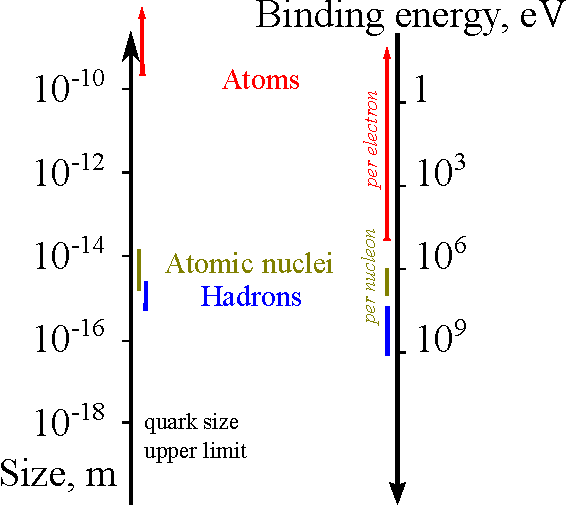
\includegraphics[height = 8cm]{illustrations/intro_illustrations/scales.pdf}
  \caption{Size and energy scales from atoms to quarks. This thesis deals in the
           range of atomic nuclei and hadrons.}
  \label{fig:scales}
\end{figure}

Heavy ions are the atoms of heavy elements (from Fe to U) with some or even all
of the electrons stripped off. Descending from larger to smaller length scale,
the physics of energetic heavy ion collisions involves atoms,
atomic nuclei, hadrons, quarks and gluons. The relevant spatial scales range
from the atomic scale of order $10^{-10}$ m down to
$10^{-16}$ m as shown in the left part of Figure \ref{fig:scales}. The
binding energy scales are demonstrated in the right part of Fig.
\ref{fig:scales} and range from eV to GeV per bound object.

The existence of atoms is of common knowledge nowadays, so atoms seem to be a
good starting point to discuss physics on smaller scales. Disassembling any
macroscopic object to smaller and smaller parts one will inevitably
arrive at atoms of one of the elements from the Mendeleev's periodic table:
hydrogen, carbon, oxygen, nitrogen, sulfur, iron, or any other of more than
110 elements. First introduced by ancient Greek philosophers Democritus and
Leucippus as purely theoretical objects, today atoms can be directly observed
in the electron microscope, moreover even manipulations with individual atoms
are possible.

Starting from Rutherford experiments (Nobel prize in chemistry 1908) it is
known that atoms have a dense nucleus, which is 1000 times smaller than the
whole atom, but contains 99.9 \% of its mass. The nucleus of size $1 -
10$ fm consists of nucleons (electrically charged protons and neutral
neutrons) bound together with energies from 1 to 8 MeV per nucleon.
Even the electrons in the inner shells of heavy elements are bound by at most
0.1 MeV per electron, so electrons can be detached from a nucleus
without destroying the nucleus itself. Initial ionization is experimentally
achieved by using strong electric fields, further ionization - by accelerating
the ions and letting them fly through thin stripping foils.

Protons, neutrons and electrons exist as well as individual particles.
Protons and electrons are stable outside of atoms (their measured average lifetime
upper bounds are larger than the age of the Universe).  Neutrons live around
880 s in average, decaying into a proton, electron and anti-neutrino. The
fact that all kinds of atoms consist of only 3 particles -
protons, neutrons and electrons - is indeed very satisfying, but it has turned
out that the whole particle zoo is much richer. Hundreds of short-living
particles were discovered during the past century in cosmic rays and in
high-energy proton-proton, proton-electron, electron-positron and other
collisions in particle accelerator experiments. The variety of discovered
particles has posed the question, which of them are fundamental and how they
can be classified.

\subsection{Elementary particles}

\begin{figure}
  \centering
  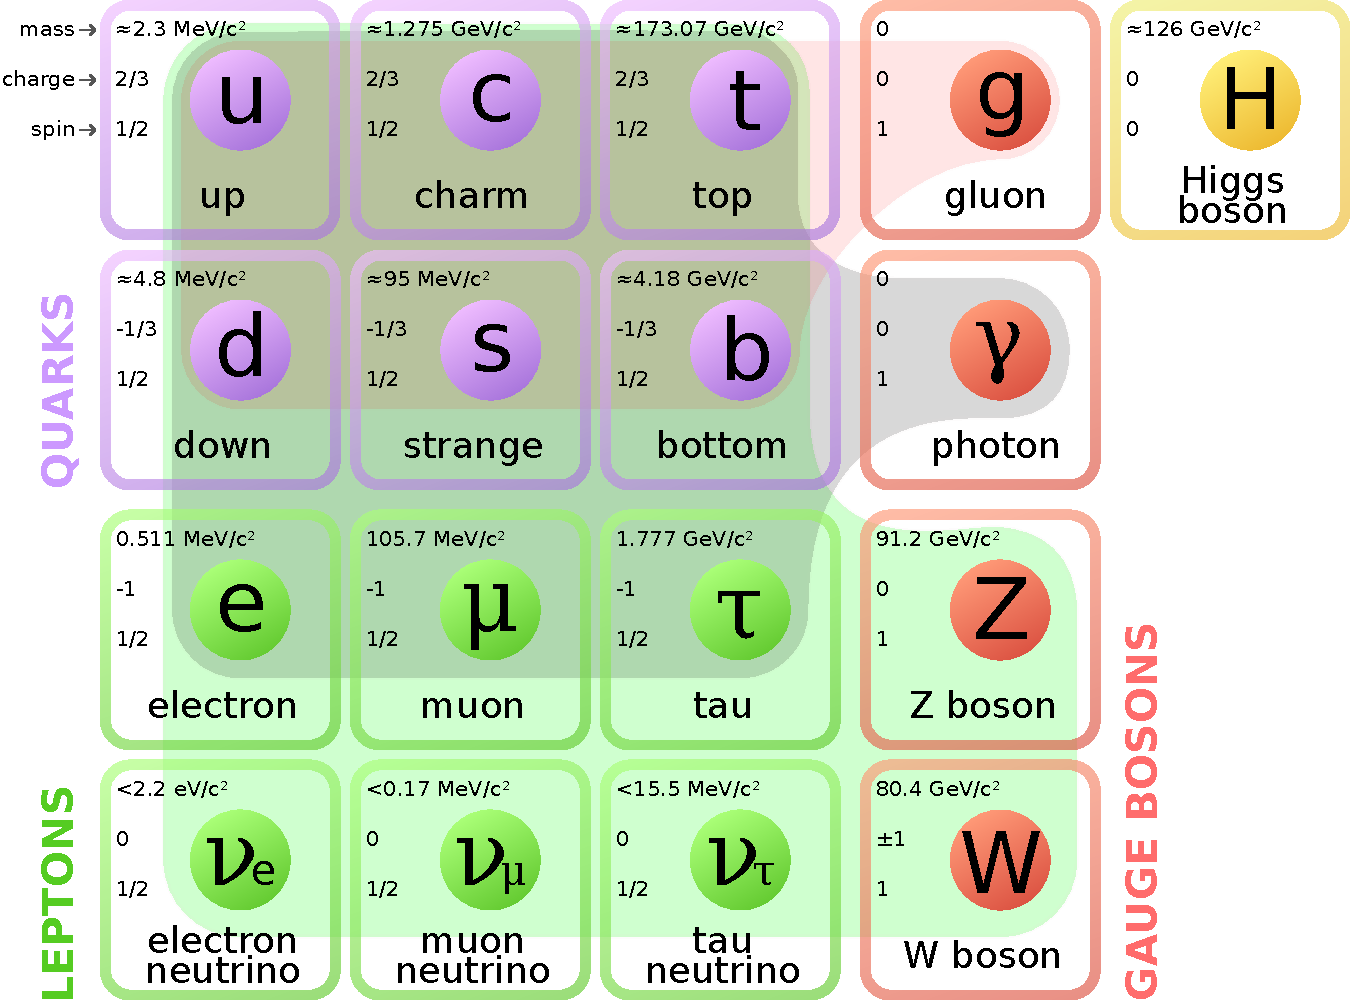
\includegraphics[width = 0.8\textwidth]{illustrations/intro_illustrations/Standard_Model.pdf}
  \caption{Elementary particles of the Standard Model, their properties and
           interactions \cite{elementary_particles_wiki}.}
  \label{fig:standard_model}
\end{figure}

Presently the above mentioned classification questions are answered by the
Standard Model of particles and interactions \cite{standard_model}.  Few
particles are considered to be elementary - by definition this means they are
point-like and do not have excited states.  Elementary particles can still be
unstable and decay into other elementary particles.  They are
characterized by mass, electric charge and spin - an intrinsic form of angular
momentum measured in units of $\hbar$. In Figure \ref{fig:standard_model} all
elementary particles are listed together with their properties according
to our present knowledge.

Depending on the spin, particles are classified into fermions (spin $\frac{1}{2}$,
$\frac{3}{2}$, $\frac{5}{2}$, etc) and bosons (spin $0$, $1$, $2$, etc). 
The difference between bosons and fermions is however not limited just to numerical
values of spin. It has a very deep
implication, manifested as the spin-statistics theorem: two fermions are not
allowed to be in the same quantum state (this rule is also referred to as Pauli
exclusion principle), while any number of bosons can be in the same quantum
state. It is due to Pauli's principle that electrons in atoms cannot reside on one
orbital, but create structures of orbitals that give elements their chemical
properties.  It also plays a role in atomic nuclei, because protons and
neutrons are fermions.  So are the quarks, of which they are composed of.

 In the Standard Model there are 12 fermions, 4 bosons with spin $1$ and the Higgs
boson with spin $0$.  All the interactions between fermions are described as an
exchange with a boson, that is why the bosons of the Standard Model are also called
force carriers. The exchange of a gluon $g$ corresponds to the strong interaction,
the exchange of $W^{\pm}$ or $Z$ bosons is the weak interaction and exchange of a
photon $\gamma$ describes the electromagnetic interaction. The Higgs boson was
introduced as a mathematical construction necessary to provide the $W^{\pm}$ and $Z$
bosons mass, which could not be introduced directly without violating gauge
symmetry.  In 2012 the Higgs boson was discovered as a physical particle. In 2013 a
Nobel prize was awarded to Englert and Higgs, who predicted the Higgs boson in 1964.


All 12 fermions in Fig. \ref{fig:standard_model} can interact weakly, i.e.
exchange $W^{\pm}$ or $Z$ bosons. However, only 6 of them interact
strongly, i.e. exchange gluons.  The strongly-interacting fermions are
called \emph{quarks}, the rest are called \emph{leptons}. Leptons include
electron, muon, tau-lepton and neutrinos. For every fermion there is also an
antiparticle, which has identical mass and spin, but opposite electric charge.
The first 3 columns of the table in Fig.  \ref{fig:standard_model} are called
generations. One can notice that  particles in each generation are
heavier than in the previous. This remains an observed fact and has no
underlying theoretical explanation.  Lighter three quarks, $u$, $d$ and $s$,
are often referred to as ''light quarks'', the rest are ''heavy quarks''. The
type of quark, one of the six possible, is also called flavour.

This thesis is devoted almost exclusively to the quark sector and the strong
interaction. The weak and electromagnetic interactions can be
neglected for the purposes of this thesis, because on the time scales of order
100 fm/c $\simeq$ $10^{-22}$ s, which are relevant for heavy ion
collisions, strong interactions are much more intense than all the
other interactions.
For example, it takes around $10^{-24}$ s to form a
pion in a proton-proton collision via strong interaction, $10^{-17}$ s
for it to decay  via electromagnetic interaction and $10^{-8}$ s to
decay via weak interaction. On the one hand, this allows to simulate heavy ion
collisions neglecting electromagnetic and weak interactions. On the other hand,
it makes photons and dileptons useful penetrating probes, which are emitted once and do not rescatter during the hadronic fireball evolution.


\subsection{Hadrons and color confinement} \label{sec:confinement}

So far, quarks and gluons were introduced as elementary particles subjected to the
strong interaction. In the following their property called ''color'' is introduced
and their bound states are discussed.

In general any particles may form bound states, if their interaction is
attractive.  For example \Pelectron and \Ppositron can form positronium,
\Pelectron and $\mu^+$ also form a bound state, connected by the electromagnetic
interaction. There are no known bound states produced purely by weak
interaction, although conjectured heavy neutrinos from extensions of the
Standard Model would form a bound state \cite{Dmitriev:2012ha}.
In contrast, strong interaction forms a plethora of bound states, called
\emph{hadrons}.

Not every combination of quarks and antiquarks appears as a bound state in
nature. Experimentally known are only $q\bar{q}$ states called \emph{mesons} and $qqq$
states called \emph{baryons}. Explaining the absence of states like $qq$ or $qq\bar{q}$
involves a property of quark called ''color''. It is unrelated
to the spectrum of reflected or transmitted light called color in our daily
life, but there is an analogy that will be explained further. Quark color has 3
eigenvalues, often denoted as $r$, $g$ and $b$. The number of colors $N_c = 3$
and the necessity to introduce it is justified by several reasons:

\begin{itemize}
\item Experimentally known hadrons like $\Delta^{++}(uuu)$ or $\Omega^-(sss)$
      would be forbidden by the Pauli principle, if the only quantum number of
      quarks was the spin. The measured spin of $\Delta^{++}$ is $3/2$, which implies
      that every $u$ quark that it is composed of has spin projection $1/2$. So
      without additional quantum numbers all $u$-quarks are in the same quantum
      state, which violates Pauli principle. With color $\Delta^{++}$ and $\Omega^-$
      are allowed by Pauli principle, because every quark is in a different color
      state.
\item A number of experiments have measured the ratio of produced hadrons
      to $\mu^-\mu^+$ pairs in \Pelectron\Ppositron collisions,
      $R = \frac{\sigma(e^+e^- \to \mathrm{hadrons})}{\sigma(e^+e^- \to \mu^+\mu^-)}$.
      This ratio is proportional to $N_c$ and measurements indicate $N_c = 3$.
\item If one takes the standard model with an arbitrary number of colors $N_c$,
      then it would be non-renormalizable because of the so-called axial anomaly in
      the electroweak sector. The anomaly is only canceled for $N_c = 3$. As a side
      note, this anomaly cancellation also requires that fermions are grouped into
      quark-lepton families.
\item All the hadrons found in nature are invariant under
      transformations in the color space, or in mathematical terms,
      hadrons are singlet representations of the $\SUgroup{3}$ group (more details are
      given in the appendix \ref{sec:SU3}). Here the
      analogy with our daily life color comes into play: like red, green and blue
      superimposed result in white, colored quarks compose ''colorless'' hadrons. Here
      ''colorless'' actually means that hadrons do not change - are invariant - under
      the $\SUgroup{3}$ transformations in color space. It turns out (see appendix
      \ref{sec:SU3} for details) that combinations $qqq$, $q\bar{q}$,
      $q\bar{q}q\bar{q}$, $qqqq\bar{q}$ have singlet representations of $\SUgroup{3}$
      group and thus can be colorless, while combinations like $qq\bar{q}$, $qq$,
      $qqqq$ or single quarks cannot be colorless by any means.
\end{itemize}

The observed existence of only colorless objects in nature is often referred to as
\emph{color confinement} or simply confinement, because the color is confined inside
of hadrons.  To acknowledge the role of color, the microscopic quantum field theory
describing the strong interaction is called quantum chromodynamics (see section
\ref{sec:QCD} for details). In addition to baryons and
mesons color confinement allows many other combinations of quarks, including the
pentaquark $qqqq\bar{q}$. Remarkably, in 2015 two kinds of pentaquarks were
discovered by the LHCb collaboration at the Large Hadron Collider at CERN
\cite{Aaij:2015tga}.

% PDG: www-pdg.lbl.gov/2015/listings/rpp2015-list-free-quark-searches.pdf
Confinement implies that no single free quark can be observed. This statement
has been tested experimentally by multiple experiments \cite{Agashe:2014kda},
measuring the cross-section for the inclusive reaction

\begin{equation}
  pp \to q(\bar{q}) X \,. \nonumber
\end{equation}

The best upper limit for the cross-section of such a reaction is currently set by the
CMS collaboration and constitutes $\sigma < $ $2.3 \times 10^{-40}$ cm$^2$.
This has to be compared to the total $pp$ cross-section, which is of order
100 mb or $10^{-25}$ cm$^2$. This implies that if single quarks
are produced in $pp$ collisions then at the maximum average rate of $10^{-15}$ per
collision. So far no single quark was observed.

Quantum chromodynamics (QCD) explains confinement in the following way.
From the lattice formulation of QCD one can obtain a phenomenological
quark-antiquark potential

\begin{equation}
  V(r) = -\frac{\alpha}{r} + \kappa r \,,
\end{equation}

which grows with distance. If one tries to separate a quark and an antiquark and
pull them apart, their interaction energy is large enough to produce a new
quark-antiquark pair out of vacuum. So, instead of a separated quark and antiquark
one obtains two mesons. This explanation does not provide a full understanding
of confinement. For example, it is still unclear under which conditions quarks
are not confined.

QCD predicts that at high collision energy the interaction between quarks becomes
small. This phenomenon is called asymptotic freedom (see section \ref{sec:QCD}). The
asymptotic freedom implies that there is a possibility to obtain deconfined quarks
at sufficiently high temperature and density.

\subsection{Quark-gluon plasma}

\begin{figure}
  \centering
  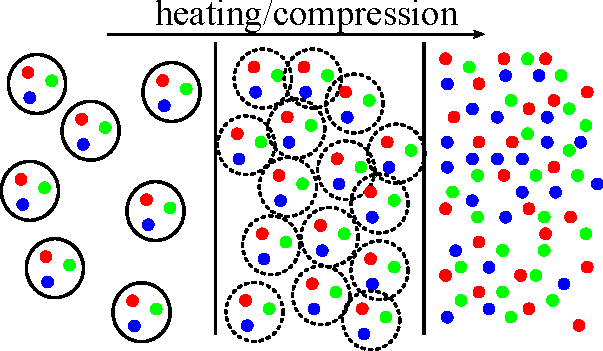
\includegraphics[width = 0.6\textwidth]{illustrations/intro_illustrations/qgp.pdf}
  \caption{Hadrons with confined color turn into a gas of quarks
           with deconfined color at heating and/or compression.}
  \label{fig:qgp}
\end{figure}

As mentioned before, it follows from asymptotic freedom of QCD that very hot
and/or very dense matter consists of almost non-interacting quarks. It
was suggested \cite{Collins:1974ky} that by heating and compressing matter in
high-energy heavy ion collisions one obtains an almost ideal gas of
\emph{deconfined} quarks. The naive illustrative picture of this is shown in
Figure \ref{fig:qgp}.

Asymptotic freedom was established theoretically in the framework of 
zero-temperature field theory for the interaction of two quarks. In a heavy ion
collision the physics is significantly different: the size of the system is much
larger than the size of a single nucleon and one can therefore speak of the formation
of a medium. Will the asymptotic freedom hold in the thermal bath created
by the medium? This question was answered by Eduard Shuryak in 1978 in the
one-loop approximation. He computed the gluon propagator and the potential
between two quarks in the thermal medium of temperature $T$ \cite{Shuryak:1977ut}:

\begin{align}
  V(r) = \frac{Q}{4 \pi r} \eexp{-m r} \\
  m^2 = \frac{1}{3} g^2 (N_c + N_f/2) T^2
\end{align}

This potential is similar to the Debye screening potential in a classical plasma,
therefore the hot and dense medium of quarks was called quark-gluon plasma.  It has
been produced experimentally at the Relativistic Heavy Ion Collider (RHIC) in 2000
\cite{Adams:2005dq,Adcox:2004mh,Arsene:2004fa,Back:2004je}.
Additionally it has been shown that the quark-gluon plasma behaves like a fluid with a
very low viscosity \cite{Song:2007ux,Dusling:2007gi,Romatschke:2007mq}. Low viscosity
implies that the QGP obtained in Au+Au collisions at RHIC is strongly-coupled, in
contrast to an earlier picture of a weakly-couple gas (see \cite{Shuryak:2008eq} for
a review of this paradigm shift).

What are the physical properties of the quark-gluon plasma? How and under which
conditions does the transition from hadronic matter to the quark-gluon plasma occur?
Is there a phase transition or only a smooth cross-over? If phase transition then of
which order? Is there a critical point and if yes, where is it located and what are
the critical indices? Are there additional phases? These are some of the
questions that motivate modern heavy ion collision experiments and theoretical
investigations. Many of these questions are directly related to the phase
diagram of the strongly-interacting matter.

\subsection{Phase diagram of strongly-interacting matter}

\begin{figure}
  \centering
  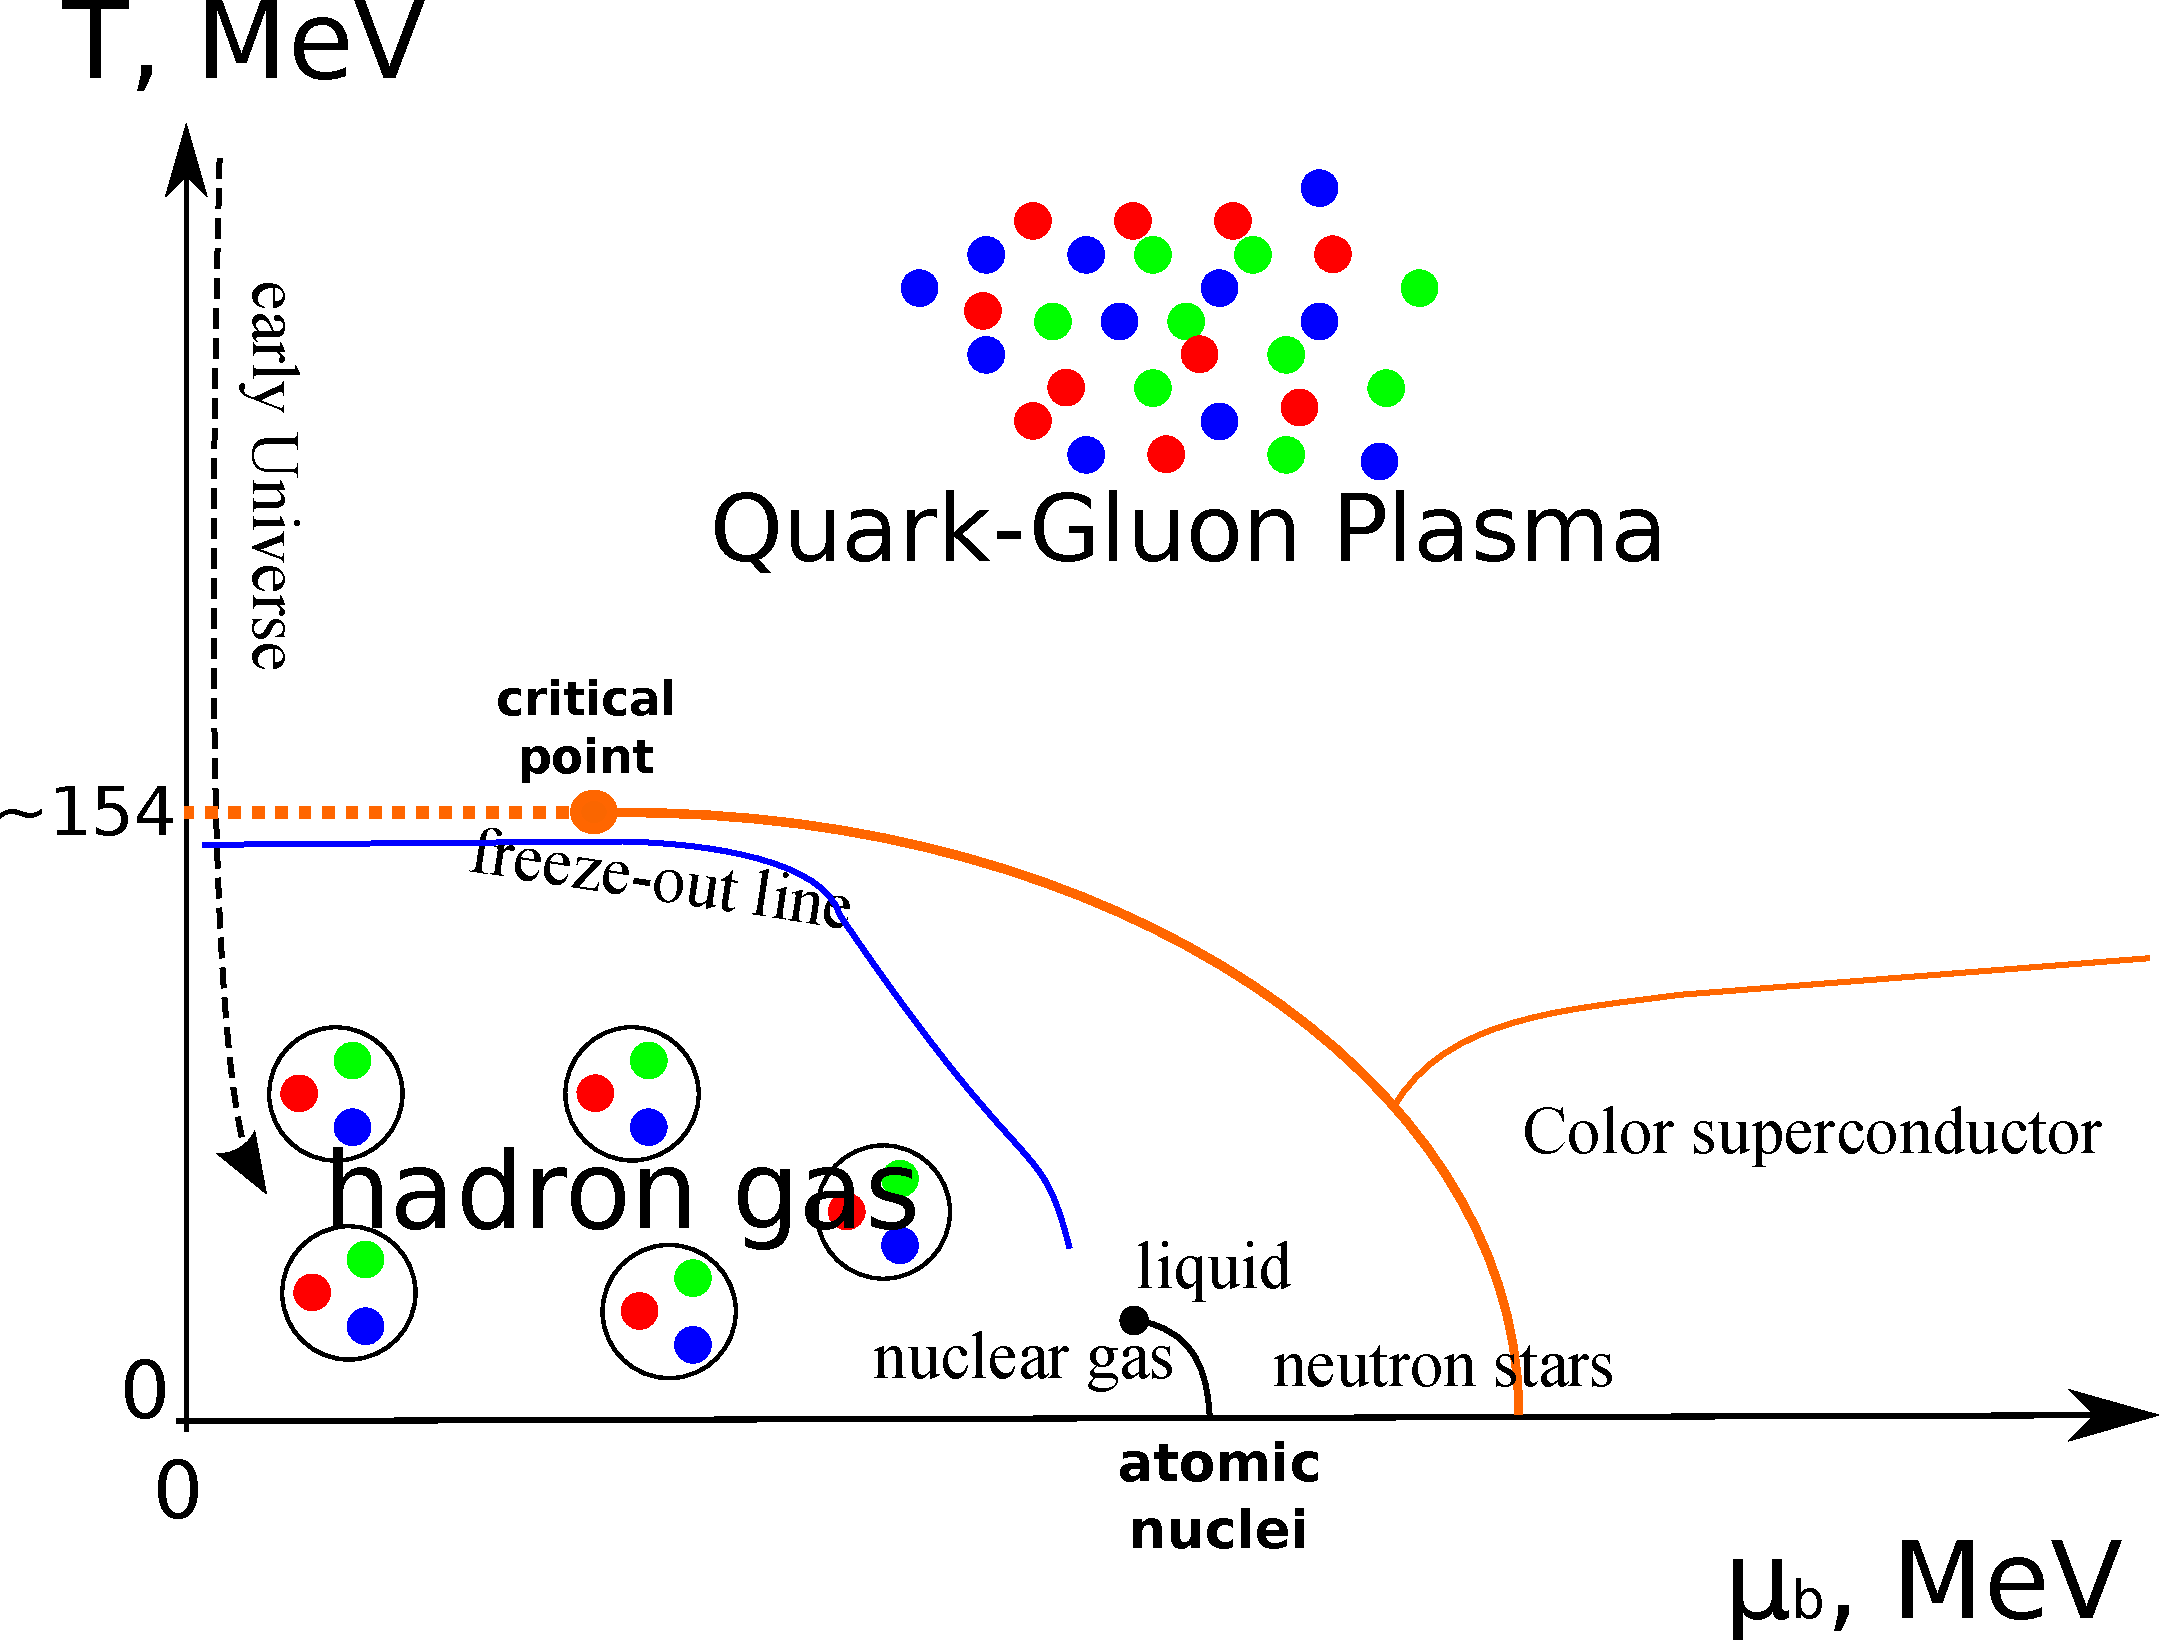
\includegraphics[width = 0.7\textwidth]{illustrations/intro_illustrations/phase_diagram.pdf}
  \caption{Schematic phase diagram of strongly-interacting matter.}
  \label{fig:phase_diagram}
\end{figure}

One of the most important tasks of modern heavy-ion collision experiments is
to study the phase diagram of strongly-interacting matter
\cite{BraunMunzinger:2008tz}. A sketch of the theoretical and experimental
knowledge about the phase diagram is given in Figure \ref{fig:phase_diagram} in
terms of temperature $T$ and baryon chemical potential $\mu_b$. The chemical potential
refers to the energy increase of the system after adding one baryon, it also
characterizes the asymmetry between baryons and antibaryons. At $\mu_b = 0$ the
energies needed to add a baryon or an antibaryon to the system are identical and
therefore baryon and antibaryon numbers are equal. At high $\mu_b$ baryons are
strongly preferred.

Strictly speaking, the diagram can have two additional axes, isospin chemical
potential $\mu_{I3}$ and strangeness chemical potential $\mu_s$. On this
diagram, it is assumed that $\mu_s=\mu_{I3} = 0$.  Non-zero isospin chemical
potential is important for neutron stars, because it characterizes the asymmetry
between protons and neutrons, which is significant in these cosmological systems.
More important for heavy ion collisions is the transition between hadron gas
and quark-gluon plasma. At high collision energies approximately equal amounts
of baryons and antibaryons are produced, so $\mu_b$ is small. The region of
$\frac{\mu_b}{T} \le 2$ is covered by lattice QCD calculations
\cite{Borsanyi:2013bia,Bazavov:2014pvz,Bazavov:2017dus}, which conclude that in
this region there is no phase transition, only a smooth cross-over.  The value
of the pseudocritical temperature where the chiral susceptibility has its maximum
is $T_c = $ 153 MeV \cite{Aoki:2006br,Borsanyi:2010bp,Bazavov:2011nk}.
Unfortunately, lattice QCD is limited to the vicinity of $\mu_b = 0$ due to
the sign problem \cite{deForcrand:2010ys}.


At non-zero $\mu_b$ a first-order phase transition is predicted by multiple
models and phenomenological studies (see summaries in \cite{Stephanov:2004wx}
and~\cite{Lacey:2014wqa}). A first order phase transition occurs in massless
two-flavour QCD \cite{Berges:1998rc,Halasz:1998qr} as well as in the two flavour
linear sigma model and Nambu-Jona-Lasinio model~\cite{Scavenius:2000qd}, in a
model based on the statistical bootstrap~\cite{Antoniou:2002xq} and in a model
with an effective potential for two-flavour massive QCD~\cite{Hatta:2002sj}.
However, none of these models can be described as fully realistic.
%Alba_realistic->complete? 
The point where the first order phase transition ends and cross-over starts is
called critical point. In the vicinity of the critical point multiplicity
fluctuations become large \cite{Stephanov:2008qz,Stephanov:1999zu}. At RHIC
and at NA61 experimental measurements of multiplicity fluctuations are ongoing
to locate the critical point. Future FAIR, NICA and J-PARC facilities have
search and possibly studies of the critical point as a part of their motivation
(see more in section \ref{sec:HI_exp}).


The nuclear matter liquid-gas phase transition with its own critical point
around $T_c^{\mathrm{nucl}} \approx $ 20 MeV was studied both
theoretically and experimentally in ion collisions
\cite{Panagiotou:1984rb,DAgostino:2005qpq}. There are many indications in
favor of a phase transition. These include temperature saturation over a broad
range of energies, flattening of the caloric curves, sudden opening of the high
fragment multiplicity channel, the onset of collective expansion, the
abnormally high partial energy fluctuations, the bimodal distribution of
exclusive observables, and the finite size and Fisher scalings. However, the
numerical value of the critical point still has a large uncertainty and even the
discovery of the transition is still debatable.

The color superconductor phase was theoretically predicted at very large baryon
densities and low temperatures \cite{Alford:1998mk,Schafer:1999fe}. At these
high densities, possibly occurring in the cores of neutron stars, gluons acquire
large mass, as quarks form a condensate and massive excitations over condensate
dominate physics, so that ''QCD at high densities and low temperatures may in
many ways be much more similar to QCD at low densities than to a weakly coupled
quark-gluon plasma'' \cite{Rajagopal:1998ec}.

The chemical freeze-out line results from an attempt to quantify features of the
phase diagram from the experimental side \cite{Andronic:2005yp}. By definition
chemical freeze-out is the instant, when inelastic number-changing hadronic
reactions cease, because of the expansion of the system, and hadron multiplicities
are fixed, ''frozen''. The thermal (also called ``hadron resonance gas'') model
postulates simultaneous sharp chemical freeze-out for all hadron species. Despite
this rough approximation, this model provides a surprisingly
good description of hadron multiplicities in heavy ion collision for collision
energies ranging from a few GeV per nucleon pair to 2.76 TeV
\cite{Cleymans:1999st,Andronic:2005yp,Stachel:2013zma}.  Temperature $T^{FO}$
and chemical potential $\mu_b^{FO}$ at the chemical freeze-out are parameters of
thermal models extracted from fitting multiplicities at each
experimental collision energy. Lattice QCD studies hint that the freeze-out curve
lies near the phase transition curve for low $\mu_b$ \cite{Kaczmarek:2011zz}.

Different parts of the phase diagram are studied with different theoretical
approaches and it is an important task to connect them. Describing different parts of
the phase diagram in a unified approach would allow
to connect properties of neutron stars, heavy ion collision experiments at
high energies and measurements of the nuclear phase transition.

\subsection{Big bang and neutron stars}

The physics of hadrons and quark-gluon plasma has deep connections to cosmology, in
particular to the early universe evolution and to neutron stars. Our universe is
known to be uniform on a very large scale of 100 Mpc, but it is extremely
non-uniform on a smaller scale. Indeed, the density of neutron star is 40
orders of magnitude larger than the density of cosmic voids. It is suggested that
the phase transition from a hot quark-gluon plasma to hadrons during the first
microseconds after the Big Bang could be partly responsible for such a non-uniformity.
For example, in \cite{Witten:1984rs} lumps of quark matter floating in
the Universe are suggested and in \cite{Kapusta:2000fe} the impact of the QCD
transition on inhomogeneities in the baryon to photon ratio is studied.

After the Big Bang the universe was extremely hot, small and was cooling and
expanding \cite{Weinberg:1977ji}, similarly to the fireball in heavy ion
collisions, although the initial temperature was higher - of order
$10^{18}$ GeV at Plank time of $10^{-43}$ s in contrast to
initial temperatures of several hundred MeV in heavy ion collisions.
At $10^{-7}$ s the Universe has already reached conditions testable in
modern heavy ion collisions experiments.  Of course, between the universe and
ion collisions there are differences in geometry. The expansion of the universe
was spherical, while heavy ion collisions have a collision axis. However, due to
the formation of a quark-gluon plasma, similarities in expansion and cooling and
also in the sequence of freeze-out processes heavy ion collisions are sometimes
called the Little Bang.

Hadronic and quark-gluon plasma physics are also related to neutron stars and
conjectured quark stars \cite{Xu:2002wd}. Neutron stars are remnants of type II
supernovae explosion, typically detected as millisecond radio pulsars. They can
neither be too light, otherwise they would be destroyed by centrifugal force;
nor too heavy to avoid collapse into a black hole. Observed neutron stars have
masses approximately between 1 and 2 solar masses and radius from 10 to 20
kilometers \cite{Lattimer:2012nd}. Simultaneous precise measurements of mass,
radius and rotation period of neutron stars would put stringent constraints on
the nuclear equation of state at high densities. For example, precise
measurements of the masses of PSR J1614-2230 ($M =  1.97 \pm 0.04 M_{Sun}$)
and PSR J0348-0432 ($M = 2.01 \pm 0.04 M_{Sun}$)
\cite{Demorest:2010bx,Antoniadis:2013pzd} have excluded many quark matter
equations of state, which could not produce such heavy neutron stars.
Nevertheless, there is still enough room for stars with quark core
\cite{Alford:2013aca,Benic:2014jia}.  Astrophysical measurements of neutron
stars probe the lower temperature and high density region of the phase diagram
in Fig. \ref{fig:phase_diagram} and are thus complementary to heavy ion
collision studies.

\subsection{Structure of the thesis}

Going from atoms to neutron stars, the introductory part of this thesis has outlined
the general motivation driving heavy ion collision experiments and theoretical
calculations all over the world. Section \ref{sec:HI_exp} overviews the
experimental studies of heavy ion collisions and demonstrates substantial
interest on intermediate energies, where the search of the critical point is or
will be performed. Section \ref{sec:HI_th} constitutes a brief overview of theory
related to heavy ion collisions. This is necessary to show the inter-relations
between different theoretical approaches and to introduce transport, hydrodynamical
and hybrid approaches, which play a big role in this thesis.

Chapter \ref{ch:interfaces} contains a mathematical part of methodology necessary
for the next parts. It provides a detailed description of the coarse-graining method,
fluidization and particlization - the interfaces between hydrodynamics and transport,
studied in this work.

The assumptions behind hydrodynamical and hybrid approaches that were fulfilled
at high energies may become challenging at intermediate energies. The first of these
assumptions is rapid thermalization over the whole fireball volume in heavy ion
collisions. The local thermalization at energies $\Elab = 5-160$ GeV per nucleon
($\sqrt{s_{NN}} = $ 3-17 GeV) is studied in a coarse-grained transport
approach in chapter \ref{chap:local_equilibration}.  The degree of
thermalization is estimated by quantifying local deviations of energy-momentum
tensor and baryon four-current in the Landau rest frame from the thermal equilibrium.
chapter \ref{chap:local_equilibration} is based on publication \cite{Oliinychenko:2015lva}.

Another assumption adopted by hydrodynamical and hybrid approaches at high
energies is that particles emitted from the region of hydrodynamical evolution
cannot return back and cause feedback to hydrodynamics. Neglection of
this feedback is typically manifested as so-called ''negative Cooper-Frye
contributions'' - negative numbers of particles emitted from certain regions of
the phase-space. At high energies at midrapidity they are negligible. Does this
hold for intermediate energies?  This question is investigated in chapter
\ref{chap:cooper_frye} based on publication \cite{Oliinychenko:2014tqa}.

Chapter \ref{chap:smash} (based on \cite{Weil:2016zrk}) introduces the SMASH
transport approach, which was used for the following computations.
In chapter \ref{chap:forced_therm} (based on \cite{Oliinychenko:2016vkg})
a novel approach to simulate hydrodynamical regime at high density
avoiding negative Cooper-Frye contributions is suggested and tested.
This approach is based on performing forced canonical thermalization in the
high-density region of the pure hadronic transport.
Chapter \ref{chap:summary} summarizes the main results of this work.

\section{Heavy-ion collision experiments} \label{sec:HI_exp}

%\begin{sidewaysfigure} \centering \includegraphics[width =
%\textwidth]{illustrations/intro_illustrations/mindmap/Heavy_ion_collisionsexperiments.pdf}
%\caption{Heavy ion collision experiments of the past (grey), present (red) and
%future (blue) with beam kinetic energy $\Elab > $ 1 GeV.}
%\label{fig:HIC_exp_mindmap}
%\end{sidewaysfigure}

\begin{table}
 \footnotesize
 \caption{Summary of heavy ion accelerators at energy $\Elab > $ 1 GeV.
          Operation time is given only for heavy ion period: e.g. Bevalac started
          operation in 1960, but heavy ion program was initiated in 1971.
          Note that only accelerated projectile ions are listed in the table, but not target
          ions.}
 \label{tab:HI_accelerators}
\begin{tabular}{llllllm{1cm}m{2cm}l}
  \toprule
  Accelerator                       &  Place                         &  Lab.  & Time       & $E_{beam}$ [GeV]    & $\sqrt{s_{NN}}$ [GeV]   & Projectile ions           & HI Experiments  & Refs.\\
  \midrule
  Bevalac                           & \pbox{20cm}{Berkley\\USA}       & BNL          & 1971-1993  & 0.4 - 2.1           & 2 - 2.7                 & O, C, Ne, Fe, Xe, U  & Plastic Ball, Streamer chamber, EOS, DLS & \cite{Barale:1975bb,Alonso:1982md} \\
  \midrule
  \pbox{20cm}{Synchro-\\Phasotron}  & \pbox{20cm}{Dubna\\Russia}      & JINR         & 1970-2003  & 0.1 - 4.5           & 1.9 - 3.5               & d - Si       &  & \cite{Malakhov:2013zjq} \\
  Nuclotron                         &                                 &              & 1993-now   & 0.1 - 4.5           & 1.9 - 3.5               & d - Xe, Au   & BM@N & \cite{Kovalenko:2016qmy,Kuznetsov:2016ynd} \\
  NICA                              &                                 &              & 2023-      & 2 - 5.5             & 4 - 11                  & d - Au       & MPD &  \cite{Kozlov:2016nbo, Kekelidze:2012zz} \\
  \midrule
  SIS18                             & \pbox{20cm}{Darmstadt\\Germany} & GSI          & 1990-now   & 0.1 - 2             & 1.9 - 2.7               & d - Au, $\pi$ & FOPI, HADES, KaoS & \cite{cbm_physics_book} \\
  SIS100(300)                       &                                 &              & 2022-      & $<$ 14 (44)         & $<$ 5.5 (9.2)           & d - U, $\pi$ & CBM, PANDA, NUSTAR & \cite{cbm_physics_book} \\
  \midrule
  AGS                               & \pbox{20cm}{Brookhaven\\USA}    & BNL          & 1980-1999  & 2 - 14.5            & 2.7 - 5.5               & O, Si, Au    & E802, E859, E866, E917, E814, E877, E810, E891, E895, E910 & \cite{cbm_physics_book, AGS_exp} \\
  RHIC                              &                                 &              & 2000-now   & 3.85 - 100          & 7.7 - 200               & Au, Cu, U, d & STAR, PHENIX, PHOBOS, BRAHMS   & \cite{RHIC_lumi} \\
  \midrule
  SPS                               & \pbox{20cm}{Geneva\\Switzerland}& CERN         & 1983-now   & 20 - 200            & 6.3 - 19.4              & O, S, In, Pb & NA35, CERES(NA45), NA49, NA57, NA60, WA98, NA61 (SHINE) & \cite{cbm_physics_book,Pugh:1989eb} \\
  LHC                               &                                 &              & 2008-now   & 1380 (Pb)           & \pbox{20cm}{2760 (PbPb)\\5400 (pPb)} & Pb & ALICE, ATLAS, CMS, LHCb & \cite{Armesto:2015ioy} \\
  \midrule
  MR                                & \pbox{20cm}{Tsukuba\\Japan}     & JPARC        & 2024-      & 1 - 19              & 2 - 6.2                 & d - U        &   & \cite{Sako:2015cqa} \\
 \bottomrule
\end{tabular}
\end{table}

An important part of the motivation for this thesis stems from ongoing and
planned heavy ion experimental programs. That is why in this section a short overview
of heavy ion experiments is given. Only experiments with the relativistic beam of
kinetic energy $\Elab > $ 1 GeV per nucleon are considered. This
condition cuts off heavy ion programs devoted to nuclear physics, such as heavy
ion experiments in Saclay (France), Uppsala (Sweden), East Lansing (USA) or
RIKEN experiment (Japan). In the world there is only a limited number of
accelerators operating at $\Elab > $ 1 GeV per nucleon, the information
about them is summarized in table \ref{tab:HI_accelerators}. They are all
synchrotrons with a beam revolving continuously in a circular beam pipe.
Typically multiple experiments are taking advantage of the beam.

% Lowest energy: Bevalac, Synchrophasotron, SIS18
Pioneering experiments in heavy ion collisions were performed in the 1970ies at
Bevalac at Lawrence Berkley Laboratory (LBL) in the US and at Synchrophasotron in
Dubna (Russia). They managed to create compressed nuclear matter and study
its properties. The most important results of Bevalac include studies of the
equation of state of nuclear matter \cite{Brown:1990pp}, collective phenomena
\cite{Doss:1986eh,Gustafsson:1984ka} and low-mass dileptons
\cite{Roche:1988er}.  Synchrophasotron studied cumulative effect,
HBT-correlations\cite{Lisa:2005dd} and nuclear multifragmentation
\cite{Kuznetsov:1982zc}.  These
experiments were operating at beam energies below 2 GeV per
nucleon. In 1990 SIS18 started to operate in the same energy regime. SIS18
experiments FOPI and KaoS have performed systematic studies of pion production
\cite{Reisdorf:2006ie}, strangeness production
\cite{Laue:1999yv,Wisniewski:2001dk} (including subthreshold production of
$\Sigma$-baryon \cite{Lopez:2007zz} and $\phi$-meson \cite{Mangiarotti:2002mw})
and collective flow studies \cite{Andronic:2000cx}.  HADES continues these
studies \cite{Stroth:2017blf} and extends them to investigations of dilepton
production \cite{Agakishiev:2011vf,Franco:2017ano}. Hadronic transport approaches were
successfully applied to describe the results of experiments at Bevalac and
SIS18.

% Low energy: AGS
Beam energies of $\Elab$ = 2 - 14.5 GeV ($\sqrt{s_{NN}} = $ 2.7 -
5.5 GeV) were covered by the Alternating Gradient Synchrotron (AGS) at
Brookhaven National Laboratory, first colliding lighter $^{16}$O and $^{28}$Si
nuclei and then heavier $^{197}$Au nuclei.  Exclusive particle spectra
\cite{Ahle:2000wq,Ahle:1999va,Ogilvie:1997mb} were measured for $\pi^{\pm}$,
$K^{\pm}$, $p$, $\bar{p}$, $\Lambda$, $\bar{\Lambda}$ and $\varphi$. Directed
($v_1$) \cite{Barrette:1995cv} and  elliptic ($v_2$) flow
\cite{Barrette:1996rs} were investigated.  Pion interferometry
\cite{Lisa:2000xj} allowed to extract the produced fireball size. The overall
conclusion was that ``there is no evidence for any onset of new behavior beyond
hadronic scattering as the beam energy or centrality is
changed''~\cite{Kahana:1997aq}, because the results of AGS were well-reproduced
by the hadronic transport models RQMD and ARC \cite{Kahana:1997aq}. Another
conclusion was that the produced particle multiplicities correspond to thermal
equilibrium in the grand-canonical ensemble \cite{BraunMunzinger:1994xr}, which
turns out to be true also for higher collision energies.

% Intermediate energy: SPS
At the Super Proton Synchrotron (SPS) at CERN a sequence of experiments
was carried out using oxygen, sulfur and lead
beams at $\Elab = $ 20-200 GeV per nucleon corresponding to
$\sqrt{s_{NN}} = $ 6.4-19.4 GeV. At the highest SPS energy NA35
experiment reached the theoretically required energy density for
quark-gluon plasma formation in S+S collisions~\cite{Pugh:1989eb}. The goal of
the later experiments in a larger Pb+Pb system was to look for the onset of
quark-gluon plasma formation by decreasing collision energy. The experiments NA45,
NA50 and WA98 measured low-mass dielectron spectra \cite{Wessels:2002ha},
dimuon spectra \cite{Ramello:2003ig} and direct photons \cite{Aggarwal:1998vs}.
NA57 has measured multistrange hadron production \cite{Bruno:2004pv}. Very
extensive and systematic measurements of hadron production were conducted by
NA49 experiment \cite{Bachler:1999hu}.  Overall, big attention at SPS was
devoted to electromagnetic and strange particle observables as potential
signals of the quark-gluon plasma formation.  Among these signals are ''Kink,
Step and Horn'' \cite{Gazdzicki:2010iv,Rustamov:2012np}: a sharp maximum in the
$\frac{K^+}{\pi^+}\parenths{\sqrt{s}}$ (Horn), sudden change in the number of
pions per participant (Kink) and a plateau in the $\sqrt{s}$ dependence of
inverse slop parameter of the kaon transverse momentum spectra (step). Hadronic
transport models were unable to describe the Horn and especially the Step
\cite{Bratkovskaya:2003ny}. This is consistent with the hypothesis of
quark-gluon plasma observation, although does not serve as unambiguous
evidence.  NA61, the successor of NA49 experiment, is now operating at the same
energies that NA49, but with a broader range of collision system sizes
\cite{Gazdzicki:2011fx}. NA61 also puts more attention to measuring hadron
multiplicity fluctuations.

%RHIC
The Relativistic Heavy Ion Collider (RHIC) at Brookhaven National Laboratory
started its operation in 2000 using AGS as a preaccelerator. The beam time at RHIC is
dedicated almost completely to heavy ion collisions (there is also a polarized
proton collision program). Unlike all the previous experiments, RHIC is a
collider. Initially experiments at a center of mass collision energy of
$\sqrt{s_{NN}} = $ 200 GeV and 130 GeV per nucleon were conducted. Later the
Beam Energy Scan program was launched with the motivation to find the critical
point of the phase diagram (see Fig. \ref{fig:phase_diagram}) and the collision
energy was systematically decreased down to 7.7 GeV at the cost of beam
luminosity \cite{RHIC_lumi}. The smallest experiment at RHIC, PHOBOS, has
measured global observables, including charged particle multiplicities, in a
large window of rapidity \cite{Alver:2010ck}.  BRAHMS, PHENIX and STAR have
performed systematic measurements of hadronic spectra
\cite{Chujo:2002bi,Kumar:2011us}, collective flow of identified hadrons
\cite{Agakishiev:2011eq,Lacey:2001va}, jet quenching, heavy flavour,
fluctuations and correlations in large Au+Au/Cu+Cu and in small d+Au
systems.  The spectra and elliptic flow of identified particles at low
transverse momentum is well-described by  ideal relativistic hydrodynamics
\cite{Kolb:2000fha,Huovinen:2001cy,Hirano:2002ds}, as well as by hydrodynamics
with hadronic afterburner \cite{Teaney:2001gc}.  This led to the statement that a
nearly ideal fluid was created at RHIC
\cite{Adams:2005dq,Adcox:2004mh,Arsene:2004fa,Back:2004je}. Viscous
relativistic hydrodynamics was applied to describe the RHIC $v_2(p_T)$ data
\cite{Song:2007ux,Dusling:2007gi,Romatschke:2007mq} and it was shown that an
extremely low viscosity to entropy density ratio $\frac{\eta}{s}$ from 0.08 to
0.2 \footnote{Dimensionless since $k_B = \hbar = c = 1$ is used, in SI has
dimension $\frac{k_B}{\hbar}$.} is preferred by data. The applicability of
hydrodynamics, early thermalization, high $v_2$ and low $\eta/s$ signal that
a strongly-interacting fluid is produced at RHIC.  Additional convincing
arguments that this fluid is indeed the quark-gluon plasma were jet quenching
\cite{Betz:2012hv}  and the scaling of $v_2$ with the number of constituent quarks
\cite{Xu:2005jt,Adamczyk:2013gv} (although constituent quark scaling being a
signature of quark-gluon plasma is debatable \cite{Lu:2006qn}).  Currently, the RHIC
beam energy scan is focused on the search of the critical point and therefore
event-by-event fluctuations of conserved charges became important observables
\cite{Adamczyk:2013dal}.

The Large Hadron Collider (LHC), which started its operation in 2010, has
contributed significantly to the field of heavy ion collisions. LHC makes use
of a specialized detector ALICE (A Large Ion Collider Experiment) dedicated to
heavy ion collisions, but also CMS (Compact Muon Solenoid), ATLAS (A Toroidal
LHC ApparatuS) and LHCb play significant role in heavy ion measurements.  LHC,
in addition to its main $p+p$ program, is colliding $Pb+Pb$ at $\sqrt{s_{NN}} =
$ 2.76 TeV, as well as $p+Pb$ at $\sqrt{s_{NN}} = $ 5 TeV.
With energy an order of magnitude higher than at RHIC, there is no doubt in the
literature that the quark-gluon plasma is produced at LHC. HBT correlation 
measurements (see \cite{Lisa:2005dd} for explanation of the method) show
that the hot and dense fireball at LHC is larger than at RHIC and leaves longer
until decoupling \cite{Aamodt:2011mr}. Fourier harmonics of $\frac{dN}{d\phi}$
were measured up to $v_6$ and are well-described by hydrodynamics. Jet
quenching turned out to be smaller than at RHIC consistently with perturbative
QCD predictions. The biggest surprise from LHC was that the smaller systems like
$p+Pb$ or high-multiplicity $p+p$ were exhibiting large $v_2$ and were
described well by hydrodynamics, which seems to be consistent with the production
of quark-gluon plasma.

Future experiments are dedicated to the search of the critical point of strongly
interacting matter and a possible phase transition between hadrons and
quark-gluon plasma. The future accelerators are FAIR (Facility for Antiproton and Ion
Research, includes SIS100 accelerators)~\cite{Spiller:2006gj} at GSI
(Gesellschaft f\"ur Schwerionenforschung) in Darmstadt, Germany; NICA
(Nuclotron-based Ion Collider fAcility)~\cite{Kekelidze:2012zz} at JINR in
Dubna, Russia; and JPARC-HI~\cite{Sako:2015cqa} at Japan Proton Accelerator
Research Complex (JPARC) in Japan. All of them concentrate on the intermediate
or lower energy region, where the critical point and the first-order phase
transition are expected.  NICA will be a collider using the existing Nuclotron as
an injector.  This will allow to increase energy to $\sqrt{s} = $
4-11 GeV, accelerating all kinds of ion beams. FAIR will be a major
addition to SIS18 accelerator at GSI, operating with fixed target at low
energies up to $\sqrt{s} = $ 4.9 GeV at a very high beam rate and with
possibility of antiproton and rare isotope beams. JPARC-HI energies are
$\sqrt{s} = $ 2-6.2 GeV and the high beam rate is planned, as for FAIR,
of order $10^{11}$ ions per cycle.

Two observations can be drawn from this brief heavy-ion experiment overview.
Firstly, the experimental interest is shifting towards lower and intermediate
energies.  This is manifested by the RHIC beam energy scan program, NA61 at
SPS, as well as future experiments FAIR, NICA and JPARC-HI.  Secondly, with
some exceptions the results of the low-energy experiments are well-described by
hadronic transport approaches and the results of high-energy experiments are
well-described by the hydrodynamics. Understanding the results of future
experiments at intermediate energies requires extending theoretical approaches
calibrated at low and high energies.

The terms ``low energy'', ``intermediate energy'' and ``high energy'' are frequently
used throughout the thesis. The ranges are defined only approximately and are
partly motivated by the experimental programs. Table \ref{tab:energies_convention}
summarizes the convention adopted in the text.

\begin{table}
  \begin{tabular}{lll}
   \toprule
    Collision energy     &   $\sqrt{s}$ [GeV]  &   Accelerators \\
   \midrule
     ``Low''             &   $\lesssim$ 4.5    & Bevalac, Nuclotron, SIS, AGS \\
     ``Intermediate''    &   $\approx$ 5 -- 20 & SPS, RHIC (BES), FAIR, NICA, JPARC \\
     ``High''            &   $\gtrsim$ 130     & RHIC, LHC \\
   \bottomrule
  \end{tabular}
\caption{Convention for the naming of energy ranges of relativistic heavy ion
         collisions.}
\label{tab:energies_convention}
\end{table}

\section{Heavy-ion collisions theory} \label{sec:HI_th}

\begin{figure}
  \centering
  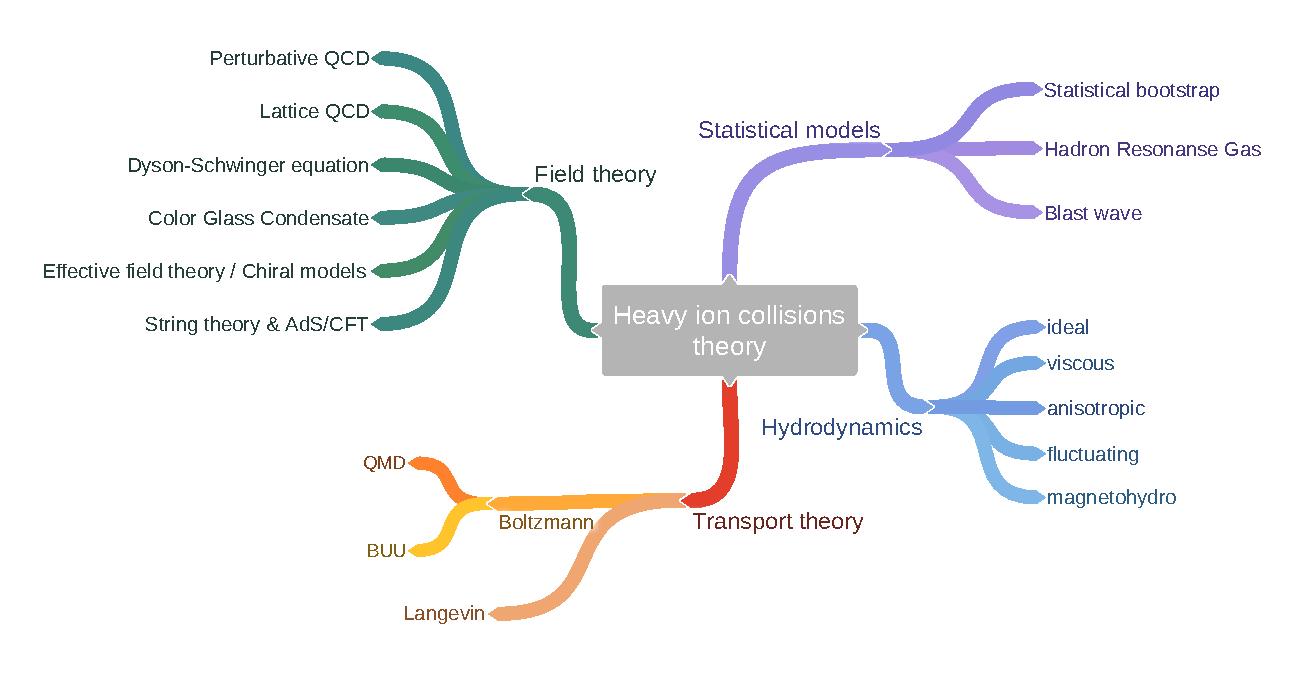
\includegraphics[width = \textwidth]{illustrations/intro_illustrations/Heavy_ion_collisionstheory.pdf}
  \caption{Theoretical approaches to heavy ion collisions.}
  \label{fig:HIC_th_mindmap}
\end{figure}


The theory of heavy ion collisions is rather versatile: the approaches range
from completely microscopic and static lattice QCD to macroscopic relativistic
hydrodynamics. The theoretical approaches may be divided into four branches as
shown in Fig. \ref{fig:HIC_th_mindmap}: field-theoretical, transport,
hydrodynamical and statistical. This thesis is devoted mainly to transport and
hydrodynamical approaches, as well as their fusion called hybrid approaches. That
is why the discussion about them is more extensive.  The other approaches are just
briefly listed here supplied with short descriptions, underlining their connections
to hydrodynamics and transport.

\subsection{Quantum chromodynamics} \label{sec:QCD}


The modern microscopic theory describing interactions of quarks and gluons is
quantum chromodynamics (QCD). Its Lagrangian is composed of interacting quark
fields $\ket{\Psi}$, which carry flavor, color and spin indices (therefore $6
\times 3 \times 4$ components) and gluon fields $A$ with Lorentz indices and a
color index taking 8 possible values corresponding to the number of
$\SUgroup{3}$ generators (see appendix \ref{sec:SU3}):

\begin{align} \label{eq:qcd_lagrangian}
  \mathcal{L} = - \sum_f \overline{\Psi}_f \sqbracs{ \gamma^{\mu} \partial_{\mu} -
                   \frac{i}{2} g \gamma^{\mu} A_{\mu}^a \lambda_a - m_f
                 } \Psi_f - \frac{1}{4} G_{\mu\nu}^a G^{\mu\nu}_a  \\
  G^{\mu\nu}_a = \partial_{\mu} A^{\nu}_a - \partial_{\nu} A^{\mu}_a +
                  f^{abc} A^{\mu}_b A^{\nu}_c
\end{align}

Here $\lambda_a$ are the Gell-Mann matrices introduced in appendix \ref{sec:SU3},
$f^{abc}$ are $\SUgroup{3}$ structure constants,
$\sqbracs{\frac{\lambda_a}{2},\frac{\lambda_b}{2}} = f^{abc}\frac{\lambda_c}{2}$.
Parameters of the QCD Lagrangian are the quark masses $m_f$ and the interaction constant $g$.
In principle, this Lagrangian contains the full description of strong interactions,
but the equations arising after quantizing it are notoriously hard to solve.
%Using QCD Lagrangian after quantization one can compute radiative corrections
%to scattering amplitudes. In QCD, as in many other quantum field theories, they
%turn out to be infinite.  To avoid infinities, the integrals are regularized by imposing a
%cut-off or other method, e.g. using $\overline{\mathrm{MS}}$ scheme. This
%procedure involves an energy cut-off scale $\mu^2$. Then counter-terms are added to
%the Lagrangian to compensate the infinity, which was cut away
%\cite{Kazakov:2008tr}. This method is called renormalization. The theory is
%called "renormalizable" if these compensating counter-terms only change the
%parameters of Lagrangian.

\begin{figure}
  \centering
  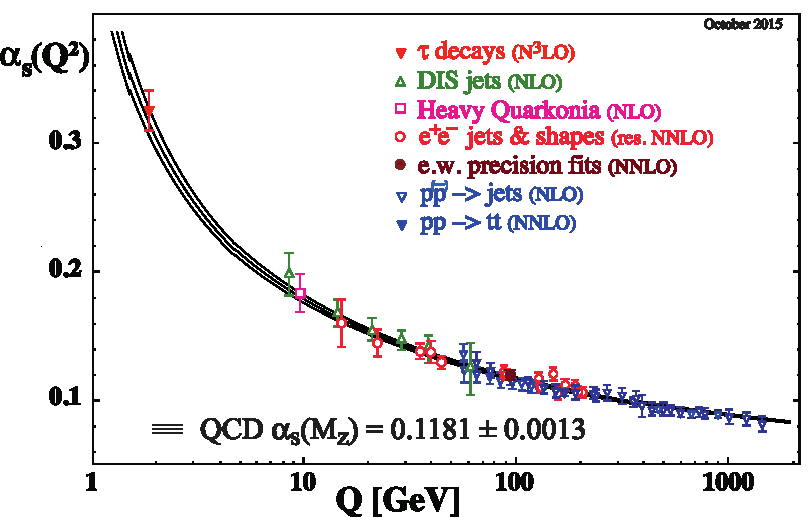
\includegraphics[width = 0.6\textwidth]{illustrations/intro_illustrations/asymptotic_freedom.pdf}
  \caption{Dependence of strong coupling constant on the energy scale. The
           decrease of coupling with energy scale is called asymptotic freedom.}
  \label{fig:asymptotic_freedom}
\end{figure}

QCD is a renormalizable theory \cite{Kazakov:2008tr} and after
renormalization the dependence of parameters $g(\mu^2)$ and $m_f(\mu^2)$ emerges,
where $\mu$ is the energy scale.
The first calculation of $g(\mu^2)$ was performed in 1973 by David Gross, Frank
Wilczek and David Politzer. They received the Nobel Prize in 2004 for this calculation.
Their main result can be expressed as follows \cite{Gross:1998jx} in terms of $\alpha_s =
\frac{g^2}{4\pi}$:

\begin{align} \label{eq:qcd_running_coupling}
  \frac{d\alpha_s}{d \, \lnOf{\mu}} = \frac{\alpha_s^2}{\pi} \beta_1 +
                                           \parenths{\frac{\alpha_s^2}{\pi}}^2 \beta_2 + \dots \\
  \beta_1 = - \sqbracs{\frac{11}{6}N_c - \frac{2}{3} n_f}
\end{align}

Here $N_c = 3$ is the number of colors and $n_f = 6$ is the number of flavors. One
 can see that $\beta_1$ is negative, so the coupling decreases with the energy scale $\mu$.
This means that the interaction between quarks at high energies or equivalently
 at small distances vanishes. This conclusion was confirmed by many
scattering experiments, see Figure \ref{fig:asymptotic_freedom}. 
The effect itself is called asymptotic freedom. Although quarks are always confined,
asymptotic freedom provides the chance to observe quasi-free quarks.
This possibility was an important motivation for heavy ion collisions,
until it has been realized that even at the highest LHC energies the quark-gluon plasma
is still strongly coupled. Indeed, the scale $\mu$ in Eq. (\ref{eq:qcd_running_coupling})
is set not by the very high collision energy $\sqrt{s}$, but by the temperature
of the formed medium, which is below 1 GeV.

Besides providing the motivation for heavy ion studies, perturbative QCD is
used to compute jet production cross-sections and jet quenching at high $p_T$
in the quark-gluon plasma. Also multiple perturbative calculations were
performed for finite-temperature QCD to determine quark-quark potentials in the
quark-gluon plasma \cite{Gross:1980br}. Perturbative calculations are
useful at high energies, where the strong-coupling constant is small according
to the Eq. (\ref{eq:qcd_running_coupling}). However, when $\mu$ decreases
the QCD coupling diverges at the scale of $\Lambda_{QCD} \sim $ 300 MeV \cite{Bruno:2017lta}.
One of the consequences is that perturbative QCD cannot deal with hadrons. This
gap is bridged by lattice QCD, described further and by other field-theoretical
approaches described in section \ref{sec:other_field_theories}.

Lattice QCD is a non-perturbative approach to QCD based on path integrals in a
discretized space-time. There are many ways to discretize the QCD action, but all
of them should converge to the same results in the continuum limit $a \to 0$
and $N_{\tau} \to \infty$, where $a$ is lattice spacing and $N_{\tau}$ is number
of points in Euclidean time. Within lattice QCD the lower lying part of the hadronic
spectrum can be computed, but most importantly for heavy ion physics it provides the
equation of state of strongly-interacting matter at zero chemical potential.
Due to Taylor expansion in $\frac{\mu}{T}$ at $\mu = 0$ the lattice QCD
equation of state is available in the region $\frac{\mu_b}{T} \le 2$
\cite{Borsanyi:2013bia,Bazavov:2014pvz,Bazavov:2017dus}. This
equation of state is widely used in hydrodynamical approaches. Lattice QCD
calculations are extremely computationally demanding, so many simplifying
assumptions are often made: large quark masses, massless quarks or small
$N_{\tau}$. Calculations with physical masses in (2+1)-flavor QCD (meaning that two
light quarks with equal masses and a strange quark are considered) and with
continuum extrapolation are only recently feasible \cite{Borsanyi:2014rza}.


\subsection{Other field-theoretical approaches} \label{sec:other_field_theories}

Field-theoretical approaches are mostly based on the QCD Lagrangian (see Eq.
\ref{eq:qcd_lagrangian}). As mentioned before, perturbative QCD cannot deal
with low-energy phenomena. This gap is partially bridged by
non-perturbative Dyson-Schwinger equations involving dressed quark and gluon
propagators \cite{Bashir:2012fs}.  They are rigorous, based on QCD and able to
capture physics at all energy scales, but unfortunately this is an infinite
system of equations that requires truncation. Other approaches covering
low-energy physics are effective field theories, where the degrees of freedom
are hadrons, not quarks or gluons \cite{Manohar:1996cq}. Such approaches are
usually based on the concept of chiral symmetry. These approaches are able to
predict hadronic cross-sections, decay widths and branching ratios, which then
can be inserted as an input to transport models. The disadvantage of effective
field theories is that they are non-renormalizable and therefore their
precision is limited and the applicability range is restricted
to low collision energies. Additionally, every hadron species needs to be inserted
should by inserted to the effective theory Lagrangian explicitly,
making realistic and detailed calculation extremely elaborate.

While chiral effective theories are applied at low energies, at high energies
the effective theory called Color Glass Condensate (CGC)
\cite{Gelis:2010nm,Iancu:2003xm} is useful. Proton-proton or nucleus-nucleus
collisions involve two energy scales: the large (''hard'') scale of the
parton-parton collision energy and the small (''soft'') scale of
inter-parton interactions within the nucleons. The computation of the reaction
cross-sections is possible within perturbative QCD for the 
parton-parton scattering. The soft part is neither accessible by perturbative
QCD nor by lattice QCD, so it is encapsulated into the parton distribution
functions (PDF) \cite{Pumplin:2002vw,Gluck:1994uf} measured mainly by
experiments at HERA $e^-p$ collider in Hamburg. PDFs depend on two parameters -
the momentum transfer $Q^2$ and the variable $x$ which
corresponds, at lowest order in perturbation theory, to the longitudinal
momentum fraction carried by a parton in the hadron. For small $x$ gluon PDFs
dominate in the nucleons, so one can say that at small $x$ nucleons consist
of a large number of gluons.

CGC is based on the concept of saturation, which can be explained as follows.
Schematically one can write a factorization theorem for the hadronic cross-sections:

\begin{equation}
  \sigma_{pp} = \int_0^1 dx_1 dx_2 \, PDF(x_1,Q^2) PDF(x_2,Q^2)
  \sigma_{partonic}\left(x_1,x_2,Q^2,\alpha_s(\mu^2),\frac{Q^2}{\mu^2}\right)
\end{equation}

The total cross-section should be limited. This follows from unitarity
\cite{Froissart:1961ux} and poses a restriction on the parton distribution function at
low $x$: PDFs should grow not faster than $\mathcal{O}\parenths{\frac{\log 1/x}{x}}$
for small enough $x$, $x < x_s(Q^2)$ - a phenomenon called saturation. Instead of
$x < x_s(Q^2)$ condition for fixed $Q^2$ one can also introduce $Q^2 > Q_s^2(x)$
condition for a fixed $x$. These considerations allow the CGC approach to separate
small $x$ and large $x$ physics. Within the CGC the nucleons are approximated as a combination of
classical gluon fields at small $x$ and valence quarks at large $x$ as sources of
these fields. The CGC picture is applicable for the very initial state of heavy ion collisions,
but at time of order $Q_s^{-1}$ the gluon medium becomes dilute and the 
basic assumption of saturation is no longer reached.  A suggested solution is to couple CGC
initialization to hydrodynamics \cite{Hirano:2005xf} or transport approaches
\cite{Kurkela:2015qoa}.

Another set of approaches to the strongly coupled regime inaccessible by
perturbative QCD is exploiting dualities between strongly coupled quantum
field theories and weakly-coupled gravitational theories, such as the  famous
AdS/CFT duality \cite{Maldacena:1997re}. This kind of approach was used to compute
the shear viscosity to entropy density ratio $\frac{\eta}{s}$ in a strongly-coupled
conformal field theory and find the well-known low value of $\frac{\eta}{s} =
\frac{1}{4\pi}$ \cite{Kovtun:2004de}.  The gauge-gravity duality has also been
applied to study the approach of fireball in heavy ion collisions to equilibrium
\cite{Chesler:2015lsa}.  Moreover, the whole heavy ion collision process at
high energies can be considered as a dual of two gravitational shock waves
colliding \cite{Arefeva:2016lcz}. Although very powerful, duality approaches
for heavy ion collisions can currently serve only for qualitative insights,
since no dual theory of QCD has yet been found.

\subsection{Statistical approaches}

Statistical approaches avoid describing the complex evolution of the fireball
in heavy ion collisions. Instead it is assumed that at chemical freeze-out all
the hadrons are in thermal and chemical equilibrium at the same temperature
$T$.  This allows to describe the fireball at freeze-out as an ideal gas of
hadrons and hadronic resonances. The inclusion of resonances as degrees of
freedom encapsulates hadron-hadron interactions according to the Bernstein-Dashen-Ma
theorem \cite{Dashen:1969ep}. The latter assumes that hadron interactions
proceed via narrow resonances, which is not always true: for example see Fig.
\ref{fig:xs} for $pp$ cross-section, which has no resonant structures.
Under the mentioned assumptions in the grand-canonical ensemble for an
ideal Boltzmann gas one obtains

\begin{equation}
  N_{i} = \frac{g_i V e^{\mu_i/T}}{2\pi^2} T^3 \parenths{\frac{m_i}{T}}^2 K_2\parenths{\frac{m_i}{T}} \,,
\end{equation}

where $N_i$ is the multiplicity of the hadron species $i$, $g_i$ is its degeneracy
and $m_i$ is its mass. This equation has to be supplied with conservation laws to
fix chemical potentials, resonance decays have to be taken into account for
comparison with experimental data and various corrections are possible - see
\cite{Andronic:2005yp,Oliinychenko:2012hj} for details. The overall model is
called Hadron Resonance Gas (HRG) model.  Although the HRG model is very simple and
its assumptions are rather naive, it describes hadron multiplicities in heavy
ion collisions remarkably well from AGS to LHC energies with three parameters:
the temperature $T$, the baryon chemical potential $\mu_b$ and the volume $V$
\cite{Becattini:2000jw,Andronic:2003zv,Andronic:2005yp,Cleymans:2005xv,Andronic:2008gu,Andronic:2011yq}.
Hadron Resonance Gas was also applied in the canonical ensemble with respect to strangeness conservation
\cite{Hagedorn:1984uy,Cleymans:1998yb,Begun:2006uu}. In the canonical ensemble
hadron multiplicities in $pp$ collisions \cite{Hamieh:2000tk}
and even $\epluseminus$ collisions \cite{Andronic:2008ev} can be described,
although for the latter the description quality is not as high.

The parameters $T(\sqrt{s})$, $\mu_b(\sqrt{s})$ and $V(\sqrt{s})$ extracted
from the fits to multiplicities at different collision energies $\sqrt{s}$
exhibit characteristic meaningful patterns.  Temperature of freeze-out $T$
increases with collision energy and saturates at around 160 MeV.
The chemical potential decreases with collision energy and goes to zero at LHC,
while the volume $V$ behaves exactly as the volume extracted from HBT radii - it
has a minimum at SPS energies. The saturation of the temperature may be explained
by the statistical bootstrap model by Hagedorn
\cite{Rafelski:2016hnq,Hagedorn:1965st}, which describes hadrons as ''bags''
being composites of one another. The bootstrap model yields an exponential hadron
spectrum and it originally predicted a limiting temperature $T_H \simeq $
150-170 MeV, above which hadrons cannot exist. This limiting
temperature was later reinterpreted as a transition temperature from hadrons to
quarks \cite{Cabibbo:1975ig}. It is believed that the value at which the freeze-out
temperature saturates is the Hagedorn temperature $T_H$ \cite{Andronic:2005yp}.

The Hadron Resonance Gas model only allows to describe hadron multiplicities. To
access momentum and rapidity spectra HRG was extended by including the overall
motion of the hadron gas. A freeze-out at some predefined hypersurface is
performed according to the Cooper-Frye formula \cite{Cooper:1974mv}. Such
models are called blast-wave models. They have the freedom to select the
freeze-out hypersurface, so there are several
modifications~\cite{Siemens:1978pb,Schnedermann:1993ws,Chojnacki:2011hb}.
Blast-wave models allow to describe transverse hadronic spectra using a common
radial expansion velocity $\beta$ common for all hadron species as an additional parameter.
Generally, blast-wave models are not able to produce higher-order flows: $v_2$,
$v_3$, etc. The description of anisotropic flow requires more involved dynamical approaches.

The temperatures $T_{kin}$ obtained from the blast wave fits to spectra are
typically lower than the temperatures $T_{chem}$ from HRG fit of multiplicities.
This is because inelastic reactions that change chemical content cease earlier than
pseudoelastic and elastic reactions that can only modify spectra. In other words,
chemical freeze-out happens earlier, when the temperature of the medium is higher.
The kinetic freeze-out, after which the spectra are not modified, occurs later.

\subsection{Hydrodynamic approaches} \label{sec:hydro_appr}

In contrast to statistical models, hydrodynamical approaches describe the
evolution of the fireball starting from thermalization until the
freeze-out.  Two necessary applicability conditions of hydrodynamics are
that every part of the system is in the vicinity of local thermal
equilibrium and the mean free path is much smaller than the system size,

\begin{equation} \label{eq:hydro_applicability}
  l_{mfp} \ll L \,.
\end{equation}

Typical expansion velocities in heavy ion collisions are comparable to the
speed of light, so the hydrodynamical theory must be relativistic.
Relativistic hydrodynamics was initiated in 1953 by the works of Landau for
multiparticle production in high-energy collisions of proton-proton,
proton-nucleus or nucleus-nucleus collisions\cite{Landau:1953gs,Belenkij:1956cd}. The
Landau model assumed high collision energy, so that two colliding nuclei are
represented as flat disks due to Lorentz contraction.  After colliding these
two disks stop completely and the resulting flat disk expands
longitudinally.  The model predicts a Gaussian rapidity spectrum, which was
indeed observed at AGS and SPS for the net charge.  At higher energies nuclei
do not seem to stop as rapidly as the Landau model assumes, but rather pass through
each other.  This is represented by the flat region of $dN/dy$ at midrapidity.
Such a situation is described well by the Bjorken hydrodynamical model
\cite{Bjorken:1982qr}, which assumes longitudinal boost invariance. The Bjorken
model allows to make a simple estimate of the energy density achieved in the
collision, which is used to judge by a comparison to the critical energy density
of $1$ GeV/fm$^3$, if the quark-gluon plasma was produced.

Modern approaches (recent overview \cite{deSouza:2015ena}) go far beyond these
approximations. However, the main equations of hydrodynamics, which are nothing
else but conservation of energy, momentum and charges, are written in the same
form as in the seminal papers of Landau \cite{Landau:1953gs,Belenkij:1956cd}:

\begin{align}
\partial_{\mu}\Tmn = 0 \\
\partial_{\mu}\jmu = 0 \,,
\end{align}

where $\Tmn$ is the energy-momentum tensor of the fluid and $\jmu$ is a
4-current of conserved charges. What has changed is

\begin{itemize}
  \item the dimensionality of the problem
  \item the equation of state (EoS)
  \item the initial conditions and event-by-event simulations
  \item the freeze-out conditions
  \item viscous corrections
\end{itemize}

In the following these aspects are described in more detail in this order.
Transverse expansion is included in (2+1)D and (3+1)D simulation. This is
important to describe transverse flow, in particular the dependence of
 $v_2(p_T)$, where $v_2$ is the second Fourier harmonics of the azimuthal angle distribution
 $\frac{dN}{d\varphi}$. Unlike the Landau or Bjorken models, these
 partial differential equations are not analytically solvable and have to
 be solved numerically.

The equation of state closes the system of hydrodynamic evolution equations,
connecting pressure with energy density and conserved charge densities:

\begin{equation}
 p = p (\epsilon, n)
\end{equation}

All the properties of the fluid are encoded in the EoS.  It is a big advantage
of the hydrodynamics that the EoS can be explicitly varied.  In this way one
can study the implications of the conjectured quark-gluon plasma to hadron gas
phase transition on the experimental observables \cite{Pang:2016vdc}. At low
$\mu_b$ the EoS is constrained by lattice QCD, but at higher $\mu_b$ it can
only be conjectured using phenomenological models.

The initial condition for hydrodynamics is the energy density $\epsilon(x,y,z)$ and
the baryon density $n_b(x,y,z)$ at a fixed time $t$ or at a fixed proper time
$\tau = \sqrt{t^2 - z^2}$, where the $z$-axis is along the beam direction.  Initial
conditions play an important role as they provide spatial anisotropies, which then
develop into momentum anisotropies $v_n$ measured in experiment. In earlier studies
initial conditions were smooth and based on the overlap geometry of the colliding
nuclei, see \cite{Huovinen:2006jp} for a review. In recent works they are
typically lumpy and generated by microscopic transport models
\cite{Petersen:2008dd,Karpenko:2015xea,Pang:2012he}, Color Glass Condensate
approach \cite{Lappi:2006xc,Schenke:2012wb}, IP-Glasma \cite{Gale:2012rq},
Monte Carlo versions of the Kharzeev-Levin-Nardi (MC-KLN)
\cite{Albacete:2011fw,Drescher:2006ca} or the Glauber model (MC-Glauber)
\cite{Miller:2007ri,Broniowski:2007nz,Loizides:2014vua}. Some approaches were
developed to classify this zoo \cite{ColemanSmith:2012ka}, but the true
initial condition is still to be found.

Because of the initial state fluctuations from collision to collision,
event-by-event calculations have to be performed. Instead of smooth averaged initial condition and
one hydrodynamic evolution one performs many simulations with different
initial conditions and then averages results.  These approaches are not
equivalent, since hydrodynamical equations are nonlinear.  Event-by-event
simulations are necessary to reproduce the higher flow harmonics, from $v_3$ up to
$v_6$ \cite{Gardim:2011xv,Auvinen:2013sba,Noronha-Hostler:2016opk}.

The earlier hydrodynamical simulations were stopped at a fixed time or proper
time, a so-called isochronous freeze-out. In modern simulations the freeze-out is
typically performed at a fixed temperature, energy density or Knudsen number.
Freeze-out is discussed in more detail in chapter \ref{chap:cooper_frye}.

In ideal hydrodynamics the energy momentum tensor in the rest frame of the fluid
element is written as

\begin{equation} \label{eq:id_fl_tmn_rest_frame}
    \Tmn_{\mathrm{ideal}} = \left(
    \begin{array}{cccc}
           \epsilon & 0 & 0 & 0 \\
           0        & p & 0 & 0 \\
           0        & 0 & p & 0 \\
           0        & 0 & 0 & p
    \end{array} \right) \,,
\end{equation}

where $\epsilon$ is local energy density and $p$ is pressure. Suppose that
the local fluid velocity is $\vec{\beta}$. Then the four-velocity takes the following form

\begin{equation}
  u^{\mu} = (\gamma, \gamma \vec{\beta}) \,,
\end{equation}

where $\gamma = \parenths{1 - \beta^2}^{-1/2}$. To boost the energy-momentum
tensor to the laboratory frame one multiplies it by Lorentz-matrices:

\begin{equation}
  \Tmn = \Lambda^{\mu}_{\alpha} \Lambda^{\nu}_{\beta} T^{\alpha \beta}
\end{equation}

\begin{equation} \label{eq:lorentz_boost_matr}
  \Lambda^{\mu}_{\nu} = \left(
    \begin{array}{cc}
           \gamma              & -\gamma \vec{\beta} \\
           -\gamma \vec{\beta} & \delta_{ij} + (\gamma - 1) \frac{\vec{\beta_i} \vec{\beta_j}}{\beta^2}
    \end{array} \right) = \left(
    \begin{array}{cc}
           u^0  &   -u^i  \\
           -u^i &  \delta^{ij} + (1+u^0)^{-1} u^i u^j
    \end{array} \right)
\end{equation}

Therefore, in the laboratory frame

\begin{equation} \label{eq:tmn_id_fluid}
  \Tmn_{\mathrm{ideal}} = \epsilon u^{\mu} u^{\nu} - p (g^{\mu\nu} - u^{\mu}u^{\nu}) \,,
\end{equation}

where $g^{\mu\nu} = \mathrm{diag}(1, -1, -1, -1)$. In ideal hydrodynamics the
four-current is a vector $(n,0,0,0)$, where $n$ is the density, boosted to the
laboratory frame:

\begin{equation} \label{eq:jmu_id_fluid}
  \jmu = n u^{\mu}
\end{equation}

Ideal hydrodynamics requires strict local thermodynamic equilibrium and
neglects possible dissipative effects. Small departures from local
equilibrium and dissipation are taken into account by  viscous
hydrodynamics. The equations of dissipative relativistic fluid dynamics
were first formulated by Eckart \cite{Eckart:1940te} and then by Landau and
Lifshitz \cite{LL_hydro}. Both were relativistic generalizations of
Navier-Stokes theory and are often referred to as first order theories. It
turned out that these generalizations are acausal, i.e. the speed of sound can
exceed the speed of light.  This was remedied in the Israel-Stewart second
order hydrodynamics \cite{Israel:1979wp}.  Recently a systematic expansion in
Knudsen number has been developed \cite{Denicol:2012cn}, which improves on the
14-moment approximation of Israel and Stewart.

Viscous hydrodynamics is applied with great success to simulate heavy ion
collisions
\cite{Teaney:2003kp,Romatschke:2007mq,Luzum:2008cw,Schenke:2010rr,Song:2007fn}.
It allows to describe anisotropic flow from $v_2$ to $v_6$ up to $p_T = $ 2.5 GeV
at RHIC and LHC, extract shear viscosity $\eta/s$ and bulk viscosity $\zeta/s$
and even some attempts to obtain the temperature dependence of $\eta/s$ from
experimental data are being made
\cite{Molnar:2014zha,Niemi:2015bpj,Karpenko:2015xea}.

A recent development is anisotropic hydrodynamics
\cite{Strickland:2014pga,Bazow:2013ifa}. Unlike the usual viscous
hydrodynamics, which is an expansion near thermal equilibrium, anisotropic
hydrodynamics expands around a non-equilibrium anisotropic state. This makes it
applicable for the early stages of heavy ion collisions, where the momentum anisotropy
is very large and conventional hydrodynamics cannot be applied.

\subsection{Transport approaches} \label{sec:transport}

The most general microscopic approaches to heavy ion collisions that consider
non-equilibrium evolution are approaches based on relativistic transport theory
\cite{de_Groot}.  Transport theory is formulated in terms of the
one-particle distribution function $\mathit{f}(t,\vec{r},\vec{p})$, which is
nothing else but the density in phase space. Assuming that the number of
particles in a given region of phase space can change only via collisions and
decays and neglecting all other sources of correlations one can write

\begin{equation} \label{eq:boltzmann}
  \frac{d\mathit{f}}{dt} = \frac{\partial\mathit{f}}{\partial t} +
                           \frac{\partial\mathit{f}}{\partial \vec{r}} \frac{p}{E} +
                           \frac{\partial\mathit{f}}{\partial \vec{p}} \vec{\nabla}U  = I_{coll} \,,
\end{equation}

where $I_{coll}$ is an expression called collision integral. This is the
non-relativistic classical Boltzmann equation, but it is nevertheless relevant for
quantum systems. It can be derived from the quantum BBGKY-hierarchy of
equations for the $N$-particle density matrix, truncating it at the two-particle
level and performing a Wigner transformation. This truncation assumes that the density
is not too high:

\begin{equation} \label{eq:transport_appl}
  \lambda_{\mathrm{Compton}} \ll l_{mfp} \,,
\end{equation}

where $\lambda_{\mathrm{Compton}} = \frac{hc}{M}$ is the Compton wavelength and
$l_{mfp} \simeq (\rho \sigma)^{-1}$ is the mean free path. This defines
the limit of applicability for the Boltzmann equation, which can however be overcome by
introducing different degrees of freedom. Another assumption made during the
truncation is the so-called hypothesis of molecular chaos:

\begin{equation} \label{eq:molecular_chaos}
  \mathit{f}_2(p_1,x_1;p_2,x_2) = \mathit{f}(p_1,x_1) \mathit{f}(p_2,x_2) \,,
\end{equation}

which implies the neglection of all phase space-correlations between particles.
The collision integral is written for the classical case as

\begin{equation}
  I_{coll} = \int \frac{d^3p_2}{E_2} \frac{d^3p'_1}{E_1} \frac{d^3p'_2}{E'_2}
          \times W(p,p_2 \to p'_1, p'_2) \times (f'_1 f'_2 - f f_2) \,.
\end{equation}

In the quantum case, the Boltzmann equation was first formulated by Uehling and Uhlenbeck and
therefore the equation is called BUU (Boltzmann-Uehling-Uhlenbeck):

\begin{equation} \label{eq:buu_icoll}
  I_{coll} =  \int \frac{d^3p_2}{E_2} \frac{d^3p'_1}{E_1} \frac{d^3p'_2}{E'_2}
          \times W(p,p_2 \to p'_1, p'_2) \times (f'_1 f'_2(1 + af)(1 + af_2) - f f_2 (1 + af'_1) (1 + af'_2)) \,.
\end{equation}

Here $a = 1$ for bosons and $a = -1$ for fermions. One can see that the quantum BUU
equation differs from the classical Boltzmann only by factors that account for
quantum statistics in the collision term.

The physical meaning of Boltzmann or BUU equations is very simple: for a given time interval $dt$
the number of particles in a phase-space cell has changed (left part) as much as
the number of particles that entered it from other cells via collisions or decays
(right part, gain term) minus the number of particles that escaped to other cells
via collisions or decays (right part, loss term). The Boltzmann equation can be
written in a manifestly covariant notation:

\begin{equation} \label{eq:Boltz}
  p^{\mu}\frac{\partial\mathit{f}}{\partial x^{\mu}} +
  m \frac{\partial K^{\mu}\mathit{f}}{\partial p^{\mu}} = I_{coll} \,,
\end{equation}

where $K^{\mu}$ is Minkowski-four-force vector. The Boltzmann equation as written above
is just for one sort of particles experiencing $2\to 2$ elastic collisions. In heavy ion
collisions one encounters hundreds of different hadrons, that can also collide inelastically,
decay and form resonances. For this case
Boltzmann equation turns into a coupled system of equations - as many equations
as hadron species. This system is generally solved via Monte-Carlo
simulations, where the particles propagate according to the equations of motion
obtained from the left hand side of Eq. \ref{eq:Boltz} and collide/decay
simulating the collision integral.

Depending on the degrees of freedom, there are pure hadronic transport codes,
used at low energies
\cite{Aichelin:1986wa,Ko:1989se,Pang:1992fg,Hartnack:1989sd,Cassing:1990dr},
approaches including hadrons and strings (e.g., RQMD \cite{Sorge:1989vt}, UrQMD
\cite{Bass:1998ca}, HSD \cite{Cassing:2000bj}, JAM \cite{Nara:1999dz}, GiBUU
\cite{Buss:2011mx}), only partons (e.g., \cite{Geiger:1991nj,Molnar:2004yh},
Zhang Parton Cascade \cite{Zhang:1997ej}, BAMPS \cite{Xu:2004mz}) or partons,
hadrons and string together, like PHSD \cite{Cassing:2008sv} or AMPT
\cite{Lin:2004en}.

Transport simulations are divided into two groups, usually called BUU
(Boltzmann-Uehling-Uhlenbeck) and QMD (Quantum Molecular Dynamics), which
differ in the treatment of potentials. BUU approaches aim at solving the one-body
BUU equations with mean-field potentials depending on the local density. The
hypothesis of molecular chaos implies that in BUU approaches all the
correlations between particles are destroyed. The QMD approach solves equations
of motion for particles with potentials depending on distances and momenta. The
QMD approach generates correlations between particles. In the case in which there are no
potentials, which is called the cascade mode, QMD and BUU approaches are
identical.

Transport approaches are extremely powerful tools to study heavy ion collisions,
because they do not require local equilibrium, simulate microscopic interactions
and allow to extract almost any experimentally observable quantity. However, they
also have some disadvantages:

\begin{itemize}
  \item Strictly speaking, transport approaches are only applicable, if the density
        is low enough, so that Eq. \ref{eq:transport_appl} is fulfilled.
  \item A lot of phenomenological input is required. Many resonance cross-sections
        and branching ratios are not known experimentally. Modeling microscopically
        the hadronization process is challenging. String formation and fragmentation
        can be modeled in many possible ways. All this creates considerable
        differences in the results even between conceptually similar approaches,
        see e.g. this comparison \cite{Xu:2016lue}.
\end{itemize}

\subsection{Hybrid approaches} \label{sec:hybrid_appr}

%\begin{figure}
%  \centering
%  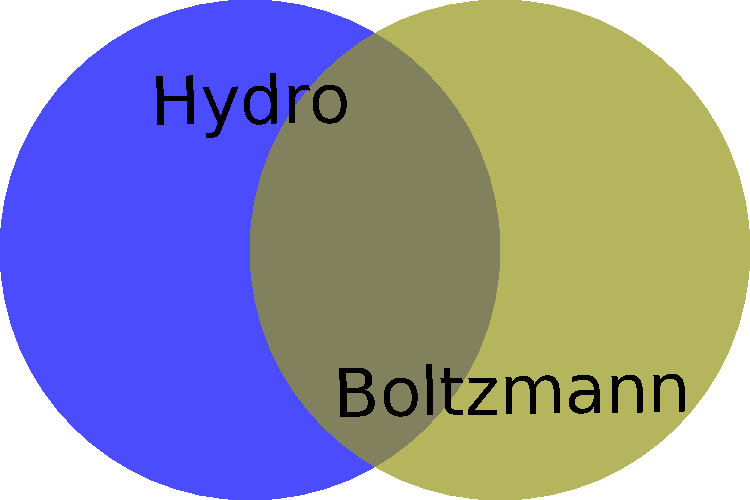
\includegraphics[width = 0.5\textwidth]{illustrations/intro_illustrations/hyd_boltz.pdf}
%  \caption{Schematic view on the regions of applicability of hydrodynamics
%           and Boltzmann equation.}
%  \label{fig:hyd_boltz}
%\end{figure}

As one can see from the applicability conditions for transport approaches (Eq.
\ref{eq:transport_appl}) and hydrodynamics (Eq. \ref{eq:hydro_applicability}),
transport tends to be applicable at lower densities and hydrodynamics at
higher densities. At the same time, the hydrodynamical equations can be derived
from the Boltzmann equation, therefore the regions of applicability of hydrodynamics
and transport overlap. 
This motivated the development of hybrid approaches, which use hydrodynamics at high
density and switch to transport at low density, hopefully in the region, where
both are applicable. Hybrid approaches are very successful in describing
experimental data at highest RHIC and LHC energies \cite{Bass:2000ib,Teaney:2001av,Hirano:2005xf,Nonaka:2006yn,Petersen:2008dd,Werner:2010aa,Song:2010mg,Karpenko:2012yf,Hirano:2012kj},
and for the RHIC beam energy scan \cite{Karpenko:2015xea,Auvinen:2016uuv}.

The advantages of hybrid approaches are:

\begin{itemize}
  \item Theoretical consistency: hydrodynamics and transport are supposed
        to be applied within their applicability ranges.
  \item The hadronic rescattering stage improves the description of experimental data
        compared to pure hydrodynamics, in particular it improves the description of
        elliptic flow $v_2$ of identified particles and
        $p_T$ spectra of protons and $\Lambda$ \cite{Petersen:2014yqa}.
  \item The equation of state can be studied explicitly.
  \item There are no uncertainties related to hadronization in the transport simulation.
        The complex hadronization process is encoded in the equation of state.
\end{itemize}

These advantages make hybrid approaches excellent simulations at intermediate
energies, relevant for RHIC beam energy scan, NICA, FAIR and JPARC. However, in
this thesis it is argued that some improvements of hybrid approaches are necessary
to perform consistent simulations at intermediate energies. These improvements
are connected to the interfaces between the hydrodynamics and transport.

Modern hybrid approaches assume:

\begin{enumerate}
  \item Fast thermalization and an ideal fluid form of energy-momentum tensor (Eq.
        \ref{eq:tmn_id_fluid}) at the initialization. At high energies these
        assumptions seem to be justified, however at intermediate energies they are
        not guaranteed. In chapter \ref{chap:local_equilibration} these
        assumptions are verified, testing the deviation of the energy-momentum
        tensor from ideal fluid form.
  \item At the initialization of hydrodynamics the whole space is assumed to be in thermal
        equilibrium. However, the borders of the fireball never really enter
        the equilibrated phase. This is cured in the core-corona approach
        \cite{Steinheimer:2011mp}, where the core with high energy density is treated
        by hydrodynamical equations and the low-density corona is propagated with
        transport. At high energies the corona is negligible, but at intermediate
        energies it becomes important. It has to be noted that in
        \cite{Steinheimer:2011mp}
        core and corona are decoupled: particles from the corona cannot feedback to
        the core.
        This is in line with the next assumption of hybrid approaches.
  \item It is assumed that transport is decoupled from hydrodynamics: particles from
        transport cannot cause any feedback to hydrodynamical equations. It turns
        out that this assumption becomes more and more challenging when one moves
        from higher energies to lower beam energies, as shown in chapter \ref{chap:cooper_frye}.
  \item The particlization hypersurface is chosen by hand. Typically, it is a hypersurface
        of constant energy density or temperature, where it is assumed that both
        hydrodynamics and transport are applicable. If this assumption is justified
        then at particlization hypersurface the amount of particles flying into
        the hydrodynamical region would be consistent with the hydrodynamical
        expectation. In chapter \ref{chap:cooper_frye} it is demonstrated that this
        conjecture is not fulfilled.
\end{enumerate}

I would like to underline that the listed assumptions are well-justified at
highest RHIC and LHC energies, where most of the hybrid approaches were applied,
but they are challenging at RHIC beam energy scan, NICA, FAIR and JPARC energies.

There is a number of approaches and ideas, which seek for relaxing these
assumptions. Anisotropic hydrodynamics \cite{Strickland:2014pga,Bazow:2013ifa}
is applicable for highly anisotropic initial states, which are out of equilibrium
in a particular way. As shown in chapter \ref{chap:local_equilibration}, the
departure from equilibrium in heavy ion collisions at intermediate energies is mainly
due to the pressure anisotropy. This means that anisotropic hydrodynamics is able to
relax the first assumption about fast thermalization.

The next assumptions could be relaxed in an approach, in which \emph{coupled}
hydrodynamical and transport equations are solved. Attempts to
write down the appropriate equations were already performed. Boundary conditions on
a sharp hypersurface separating two transport approaches with different
distribution functions were formulated in \cite{Bugaev:2002ch}. These conditions
are also suitable for the boundary between hydrodynamics and transport. However, it is not
enough to formulate the boundary conditions. One also has to supply the rules for
how particles thermalize or how they deposit energy entering the hydrodynamical
phase.

This was partially addressed in the hydrokinetic approach
\cite{Sinyukov:2002if,Akkelin:2008eh}, where particles decouple from
hydrodynamics continuously governed by rate equations. The decoupling
hypersurface is momentum dependent in such a way that particles do not
return to the hydrodynamical domain. There is also an approach of a transition
layer \cite{Csernai:2004pr,Molnar:2005gx}, where particle escape probabilities
are also governed by rate equations and particles returning to the hydrodynamical
domain are integrated out.

An approach, where coupled hydrodynamical and transport equations are solved and the
boundary is defined dynamically is not fully developed for the relativistic case.
However, the analogous non-relativistic problem often appears in practice and is solved
for many different scenarios. A possible example is the simulation
of fluid flow with complicated boundary conditions: at the boundary the fluid has
to be simulated kinetically and far from the boundary hydrodynamically.
This kind of non-relativistic problem is successfully solved using
the domain decomposition methods, see for example \cite{Tiwari:2009} and references
therein. Similar ideas are also used in plasma simulations, see
e.g.~\cite{Tuckmantel:2010}. An analogous approach for heavy ion collisions
would solve many of the problems that appear in the present hybrid models,
in particular the problem of negative Cooper-Frye contributions (section
\ref{sec:cf_explanation}).

In chapter \ref{chap:forced_therm} an alternative approach to the problem is
suggested. Hadronic transport is applied in the whole space, but in the region of
high energy density it is subjected to forced thermalization. This allows
to interpolate between transport and hydrodynamics. Unfortunately, varying
the equation of state in this approach is challenging, although possible in
principle. 	Hadrons inside the ''hydrodynamical'' high-density region
need then to be treated as fictitious particles like in the particle-in-cell
hydrodynamics \cite{Harlow:1976}.


  \chapter{Interfaces between hydrodynamics and transport} \label{ch:interfaces}

As one can see from the discussion about hydrodynamical and hybrid models, many
uncertainties in the dynamical simulations of heavy ion collision are coming from
interfaces between different approaches - for hybrid models this is the construction of
the initial state (fluidization) and final state (particlization). In this chapter the
actual calculations at these interfaces are discussed to better understand the source
of uncertainties and to introduce the methodology used in the next chapters.
Some parts of this chapter follow publications \cite{Oliinychenko:2014tqa},
\cite{Oliinychenko:2015lva} and \cite{Oliinychenko:2016vkg}.

\section{Coarse-graining} \label{sec:coarse_graining}

\begin{sidewaysfigure}
  \centering
  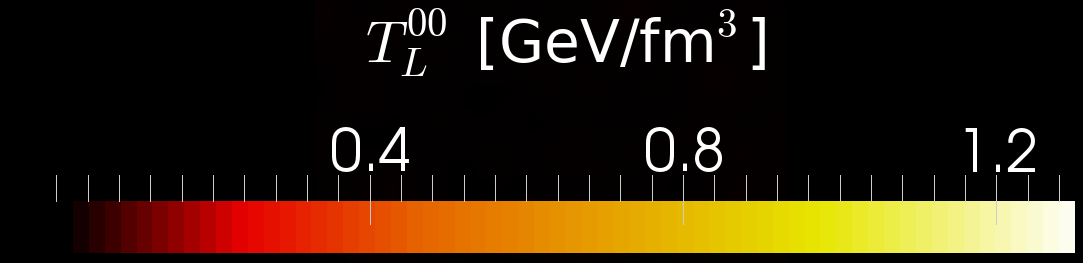
\includegraphics[width = 0.3\textwidth]{illustrations/coarse_graining/color_legend_T00.png} \\
  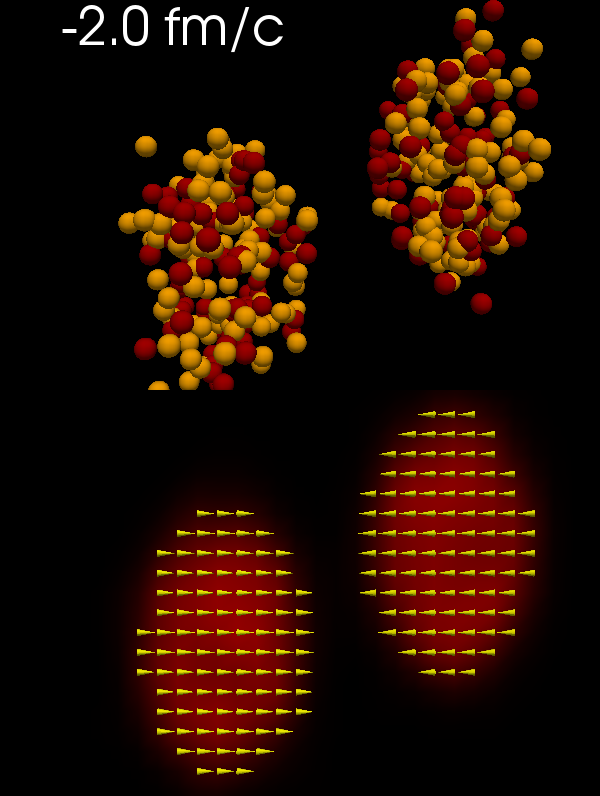
\includegraphics[width = 0.32\textwidth]{illustrations/coarse_graining/coarse_AuAu_sqrts3GeV_b5_0000.png}
  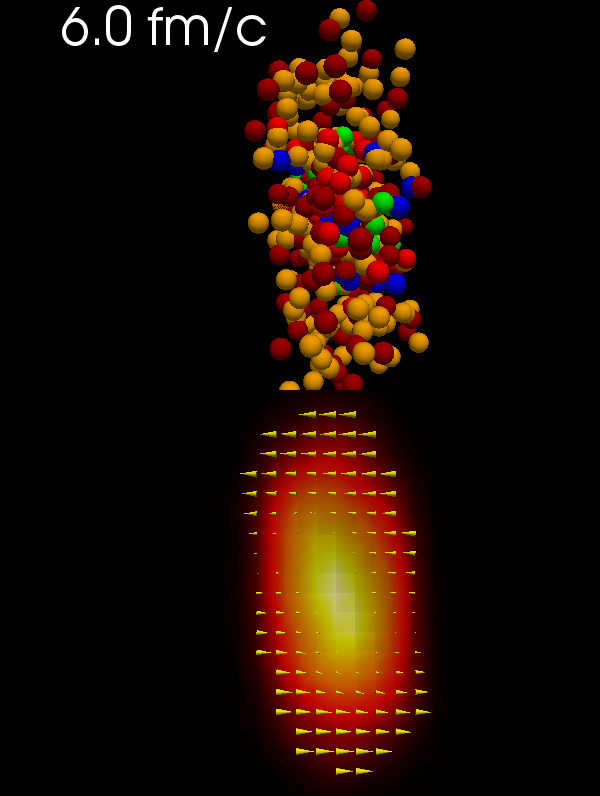
\includegraphics[width = 0.32\textwidth]{illustrations/coarse_graining/coarse_AuAu_sqrts3GeV_b5_0004.png}
  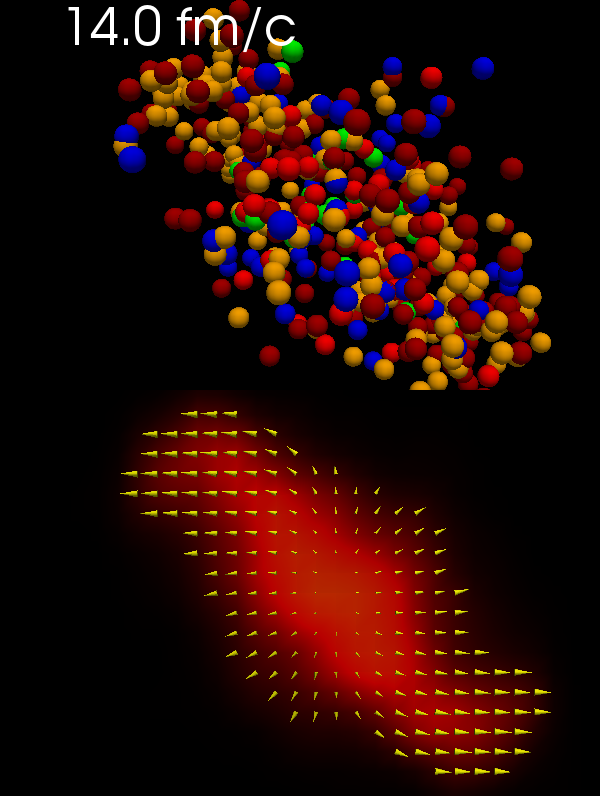
\includegraphics[width = 0.32\textwidth]{illustrations/coarse_graining/coarse_AuAu_sqrts3GeV_b5_0008.png}
  \caption{Demonstration of coarse-graining. On the top row is the particle
           representation of a Au+Au
           collision at $\sqrt{s} = $ 3 GeV and impact parameter $b = $
           5 fm from the transport code SMASH. The simulation was performed in the
           center of mass frame, that is why both nuclei are Lorentz-contracted.
           Dark-red corresponds to protons,
           yellow to neutrons, blue to pions, red to $\Delta$s and green to the rest.
           At the bottom is the coarse-grained picture of the energy-density in the
           Landau rest
           frame and Landau velocities in the XZ plane from a SMASH simulation with
           $N_{test} = 30$.}
  \label{fig:HIC_exp_mindmap}
\end{sidewaysfigure}

Coarse-graining is a method to obtain macroscopic variables, such as
the rest-frame energy-density, baryon density or velocity of the fluid from
the particles in a transport approach. This method is used extensively in chapters
\ref{chap:local_equilibration}, \ref{chap:cooper_frye} and \ref{chap:forced_therm}, as
well as in other works, e.g. \cite{Huovinen:2002im,Endres:2014zua}.
An example of coarse-graining is demonstrated in Fig. \ref{fig:HIC_exp_mindmap},
where the microscopic particles from a transport simulation of heavy ion collision are
turned into energy-density, pressure and velocity, the macroscopic variables necessary
for hydrodynamics.

In the following sections the mathematical expressions for coarse-graining are derived,
starting from the energy-momentum tensor and four-currents for a point-like particle,
and proceeding with a smeared particle or a wavepacket.

\subsection{Energy-momentum tensor of a point-like particle}

The expression for the energy-momentum tensor of a single point-like particle is
well-known in the literature \cite{LL_ED}, as well as for particles interacting
with fields \cite{Sutherland:2015}. Here the derivation is repeated to use it
later for the wavepacket.

The action of a point-like particle is

\begin{equation}
  S = -m \int_a^b d\tau = -m \int_a^b \sqrt{dx^{\mu}dx_{\mu}} \,.
\end{equation}

Varying the particle trajectory $x^{\mu} = x^{\mu} + \delta x^{\mu}$ with
fixed ends one obtains an action variation:

\begin{align}
  \delta S = -m \int_a^b \sqrt{dx^{\mu}dx_{\mu} + 2 dx^{\mu} d\delta x_{\mu}} +
             m \int_a^b \sqrt{dx^{\mu}dx_{\mu}} = \nonumber \\
             = -m \int_a^b \frac{dx^{\mu}}{d\tau} d\delta x_{\mu} = \nonumber \\
             = m \int_a^b \frac{du^{\mu}}{d\tau} d\tau \delta x_{\mu} \,,
\end{align}

where $u^{\mu} = \frac{dx^{\mu}}{d\tau}$. Using the expression

\begin{equation}
  \frac{du^{\mu}}{d\tau} = \frac{\partial u^{\mu}}{\partial x^{\nu}} \frac{\partial x^{\nu}}{\partial \tau}
   = u^{\nu} \partial_{\nu} u^{\mu}
\end{equation}

one can rewrite the action variation as

\begin{equation}
  \delta S = m \int_a^b u^{\nu} \partial_{\nu} u^{\mu} d\tau \delta x_{\mu} \,.
\end{equation}

In this expression variation of the action depends on the coordinates and velocity
of the particle, that will further be marked with index ``p''. Now let us rewrite
it in terms of continuous medium by adding integration over space-time and a $\delta$-function. The coordinates $x^{\mu}$ are coordinates in
space, over which integration is performed.

\begin{equation} \label{eq:ds}
  \delta S = m \int dV \int_a^b d\tau \delta^{(4)}(x^{\mu} - x^{\mu}_p(\tau)) u^{\nu} \partial_{\nu} u^{\mu} \delta x_{\mu} \,.
\end{equation}

The delta-function $\delta^{(4)}(x^{\mu} - x^{\mu}_p(\tau))$ allows to change
variables depending on $x^{\mu}_p$ to variables dependent on $x^{\mu}$. Since
$\int d\tau \delta(x^{0} - x^{0}_p(\tau)) = \frac{1}{u^{0}}$,
one can rewrite the equation (\ref{eq:ds}) in the following form:

\begin{align}
  \delta S = \int dV \, \partial_{\nu} \Tmn \delta x_{\mu}   \,,
\end{align}

where the following notation is used

\begin{align}
  \Tmn = m \jmu u^{\nu} \,, \\
  \jmu = u^{\mu} \delta^{(4)}(x^{\mu} - x^{\mu}_p(\tau)) = \frac{u^{\mu}}{u^{0}} \delta^{(3)}(x^{i} - x^{i}_p(\tau)) \,.
\end{align}

Here it was taken into account that $\partial_{\mu} \jmu = 0$ due to the
equations of motion. It is convenient to rewrite this in terms of the
4-momentum $p^{\mu}$ of the particle:

\begin{align} \label{eq:tmn_pointlike}
  \jmu = \frac{p^{\mu}}{p^0} \delta^{(3)}(x^i - x^i_p(\tau)) \\
  \Tmn = \frac{p^{\mu}p^{\nu}}{p^0} \delta^{(3)}(x^i - x^i_p(\tau))
\end{align}

There is a simpler way to obtain the same formulas. One notices from the
 $\Tmn$ of the ideal fluid that for a particle at rest

\begin{equation}
  \Tmn_{\mathrm{rest}}(\vec{x}) = \mathrm{diag}(m \delta^{(3)}(x^i - x^i_p), 0, 0, 0)
\end{equation}

Notice that the $\delta$-function has dimension of fm$^{-3}$ here. Boosting the
energy-momentum tensor with the 4-velocity $u^{\mu}$ using the Lorentz boost matrices
from Eq. (\ref{eq:lorentz_boost_matr}) one obtains

\begin{equation}
  \Tmn(\vec{x}') = \Lambda^{\mu}_0 \Lambda^{\nu}_0 m \delta^{(3)}(x'^i - x'^i_p)
                   \frac{1}{u^0}
           = \frac{p^{\mu}p^{\nu}}{p^0} \delta^{(3)}(x'^i - x'^i_p) \,.
\end{equation}

Note that the necessary $\frac{1}{u^0}$ factor is obtained via the $\delta$-function transformation:

\begin{align}
  d^3x \delta^{(3)}(x^i - x^i_p) = d^3x' \delta^{(3)}(x'^i - x'^i_p) \,, \\
  d^3x  = u^0 d^3x' \,.
\end{align}

The primed coordinates $x'$ here are the lab frame coordinates in contrast to
the ones in the rest frame. For $\jmu$ the calculation is analogous.

\subsection{Energy-momentum tensor of a wavepacket} \label{sec:tmn_wavepacket}

As one can see from Eq. (\ref{eq:tmn_pointlike}), for finite numbers of point-like
particles  the energy-momentum tensor will be non-zero only at the particle
positions. For coarse-graining it is desirable that $\Tmn$ is continuous in
space. That is why the point-like particles are not used directly. Instead they
are smeared, which may be physically interpreted as wavepackets in coordinate space.

To introduce a non-pointlike particle one simply replaces the $\delta$-function in
space by a smearing kernel $K(\vec{x} - \vec{x}_p, u^{\mu}_p, \sigma)$, which
represents the shape of the wavepacket in the rest frame. The smearing kernel should
satisfy three conditions: $K(\vec{r})d^3r$ should be Lorentz scalar, it should be
normalized as $\int K(\vec{x} - \vec{x}_p) d^3x = 1$, and it should approach a
$\delta$-function when the smearing parameter $\sigma$ approaches zero. Then
transforming from the particle rest frame

\begin{align}
  \Tmn_{\mathrm{rest}}(\vec{x}) = \mathrm{diag}(m K(\vec{x} - \vec{x}_p), 0, 0, 0) \\
  \jmu_{\mathrm{rest}}(\vec{x}) = \mathrm{diag}(K(\vec{x} - \vec{x}_p), 0, 0, 0)
\end{align}

exactly as it was done with the $\delta$-function, one obtains:

\begin{align} \label{eq:one_part_tmn}
  \jmu(\vec{x}') = \frac{p^{\mu}}{p^0} K(\vec{x}' - \vec{x}'_p(\tau)) \\
  \Tmn(\vec{x}') = \frac{p^{\mu}p^{\nu}}{p^0} K(\vec{x}' - \vec{x}'_p(\tau)) \,.
\end{align}

Surprisingly, all current popular choices of $K$ in the literature are such that
$K(\vec{r})d^3r$ is not a Lorentz scalar:

\begin{itemize} %[noitemsep]
  \item Cell averaging: $K(\vec{x}) = \begin{cases} 1/\Delta V, \, \vec{x} \in \Delta V \\
                                                  0, \text{otherwise} \end{cases}$.
        Here $K(\vec{x})d^3x$ is not a Lorentz scalar,
        since the volume $\Delta V$ is not contracted.
  \item Gaussian distribution with Lorentz contraction in z direction:
        $K(\vec{x}) = N exp\left(-\frac{x^2 + y^2 + \gamma_z^2 z^2}{2 \sigma^2} \right)$
        is behaving properly only under boosts in z direction.
  \item Gaussian in $x$, $y$, $\eta$ coordinates also behaves
        properly only under boosts in z direction.
\end{itemize}

Let us derive a simple, not too computationally demanding kernel, which
satisfies all aforementioned conditions, in particular $K(\vec{x} - \vec{x}_p)d^3x$
being a Lorentz scalar. In the rest frame of the particle a Gaussian is taken, assuming
that the particle is at the origin, $\vec{x}_p = 0$:

\begin{equation}
  K_{rf}(\vec{x}) = (2\pi \sigma^2)^{-3/2} exp(-\vec{x}^2/2\sigma^2)
\end{equation}

Let us now express the rest frame coordinates through coordinates $\vec{x}'$ in the
laboratory (computational) frame via the Lorentz boost using the matrix from
Eq. (\ref{eq:lorentz_boost_matr}).

\begin{align}
  \left( \begin{array}{c}  t \\ x^i \end{array} \right)
  = \left( \begin{array}{cc}
           u^0  &  u^i  \\
           u^i  &  \delta^{ij} + (1+u^0)^{-1} u^i u^j
    \end{array} \right)
  \left( \begin{array}{c}  0 \\ x'^j \end{array} \right)
\end{align}

The time component on the right hand side is zero because the smearing kernel
needs to be evaluated at a fixed time in the computational frame,
not in the particle rest frame. This derivation is analogous to the
standard derivation of the Lorentz contraction, but the direction of contraction
is not necessarily along a coordinate axis.

It follows then that

\begin{align}
  x^i = (\delta^{ij} + (1+u^0)^{-1} u^i u^j) x'^j = x'^i + (1+u^0)^{-1} u^i (u^j x'^j) \\
  \vec{x}^2 = x^i x^i = \vec{x}'^2 + 2 (1+u^0)^{-1} (u^i x'^i) (u^j x'^j) + (1+u^0)^{-2} (u^i u^i) (u^j x'^j)^2 = \\
  = \vec{x}'^2 + (u^j x'^j)^2 (1+u^0)^{-1} \parenths{2 + \frac{(u^i u^i)}{1+u^0}}
\end{align}

It follows from  $u^{\mu} u_{\mu} = 1$ that $u^i u^i = u_0^2 - 1$ and

\begin{equation}
  (1+u^0)^{-1} \parenths{2 + \frac{(u^i u^i)}{1+u^0}} = 1 \,.
\end{equation}

Therefore,

\begin{equation}
  \vec{x}^2 = \vec{x}'^2 + (u^j x'^j)^2
\end{equation}

and the kernel $K$ can be written in the computational frame as

\begin{equation} \label{eq:smearing_kernel}
  K(\vec{x}' - \vec{x}'_p, u_p, \sigma) = \frac{u_0}{(2\pi \sigma^2)^{3/2}}
  \expOf{-\frac{\vec{x}'^2 + (\vec{u} \vec{x}')^2}{2\sigma^2}}
\end{equation}

This is the kernel used for all calculations throughout this thesis.
The factor $u_0$ was added to ensure  $ K(x' - x'_p) d^3x' = K_{rest}(x - x_p)
d^3x_{rest}$, since $d^3x' = u_0^{-1} d^3x_{rest}$. Let us check explicitly
that the normalization condition is fulfilled. Using the Gaussian integral

\begin{equation}
  \int \left( \prod_{i=1}^{n} dx_i \right) e^{-x_i A^{ij} x_j}  = \pi^{n/2} \, (det A)^{-1/2}
\end{equation}

and the fact that the determinant $det(\delta_{ij} + u_i u_j) = u_0^2$ one
indeed finds that

\begin{equation}
  \int K(\vec{x}' - \vec{x}'_p) d^3x' = 1 \,.
\end{equation}

It is not a coincidence that the smearing kernel is correctly normalized.
It already follows from the transformation properties, that if it is
normalized in one frame, it is normalized in any frame. One can check that this
formula turns into the more familiar expression from \cite{Huovinen:2012is}, if
the particle velocity is directed along the z-axis and $\vec{u} = \gamma_z(0, 0,
\beta_z)$. Since $1 + (\gamma_z \beta_z)^2 = \gamma_z^2$, it follows that
$\vec{x}'^2 + (u^j x'^j)^2 = x'^2 + y'^2 + \gamma_z^2 z'^2$ and the coincidence
of the expressions is established.

The last thing to check is that the smearing kernel approaches the $\delta$-function
at $\sigma \to 0$. If this is true in the rest frame, it is true in any frame,
so is enough to check it at the rest frame. This can be immediately seen from
 the $\delta$-function limit representation

\begin{equation}
  \delta(x) = \lim_{\epsilon \to 0} \frac{1}{\sqrt{2 \pi \epsilon}} e^{- \frac{x^2}{2\epsilon}} \,.
\end{equation}

Taking this limit for every dimension one obtains

\begin{equation}
  \lim_{\sigma \to 0} K_{rest}(\vec{x} - \vec{x}_p, \sigma) =
  \delta^{(3)}(\vec{x} - \vec{x}_p) \,.
\end{equation}

Finally one notes that the exponential form of the smearing function is by no
means unique. Any normalized function of $\vec{x}'^2 + (u^j x'_j)^2$ can be
incorporated given that in some limit it gives the $\delta$-function. The reasons to
prefer an exponential are firstly, because it has infinite number of continuous
derivatives and secondly, because it corresponds to the physical background of the Gaussian wavepacket.  An alternative smearing kernel could be, for example,

\begin{equation}
  K_{\mathrm{alternative}} = \begin{cases}
    \frac{15 u_0}{8 \pi \sigma^3} \parenths{1 - \frac{\vec{x}'^2 + (\vec{u} \vec{x}')^2}{\sigma^2}} & |x| < \sigma \\
    0  & |x| > \sigma
 \end{cases}
\end{equation}

\subsection{Final expressions for coarse-graining} \label{sec:final_coarse_graining}

The derivations from the two previous sections allow to write down the expressions used
in this work for the coarse-graining. Suppose that particles for coarse-graining are
taken from $N_{ev}$ events ($N_{ev}$ transport simulations). Then the following
expressions are valid:

\begin{align}
  \Tmn(\vec{r}) = \frac{1}{N_{ev}} \sum_{events} \sum_i
                  \frac{p^{\mu}_i p^{\nu}_i}{p^0_i} K(\vec{r} - \vec{r_i}, u_i) \\
  \jmu(\vec{r}) = \frac{1}{N_{ev}} \sum_{events} \sum_i
                  \frac{p^{\mu}_i}{p^0_i} K(\vec{r} - \vec{r_i}, u_i) \\
  K(\vec{r} - \vec{r_i}, u, \sigma) = \frac{u_0}{(2\pi \sigma^2)^{3/2}}
                  \expOf{-\frac{(\vec{r} - \vec{r_i})^2 +
                                (\vec{u} \cdot (\vec{r} - \vec{r_i}))^2}{2\sigma^2}} \\
  u^{\mu} = (u^0, \vec{u}) = \frac{p^{\mu}}{m}
\end{align}

These expressions in principle allow to compute the energy-momentum tensor and
four-currents on any irregular grid, but in this work only Cartesian grids are used.

\section{Fluidization} \label{sec:fluidization}

The first interface in hybrid approaches is the transition from transport to fluid,
called fluidization. At fluidization microscopic particles with their coordinates and
momenta have to be converted into a macroscopic continuous hydrodynamic fields: density,
energy density, pressure, etc. In the relativistic case the first step of the
fluidization is the construction of the energy-momentum tensor $\Tmn$ and four-currents
$\jmu$ as describe above. However, it is by no means guaranteed that they have an ideal
fluid-dynamical form or that they are close to it. Indeed, transport
approaches generally simulate non-equilibrium systems and the $\Tmn$ of hydrodynamics
is close to equilibrium. The problem of matching a non-equilibrium $\Tmn$
to an equilibrium one is relevant for many approaches that construct their initial state
from the discrete degrees of freedom \cite{Petersen:2008dd,Skokov:2005ut,Werner:2010aa,
Andrade:2005tx,Gale:2012rq,Karpenko:2015xea,Pang:2012he,Bhalerao:2015iya}.

This matching problem can be eliminated or minimized by waiting until transport
approach reaches equilibrium and only switching to hydrodynamics, when the necessary
degree of equilibration is reached. However, it was argued that a good description of
experimental data requires rather small initialization times of hydrodynamics
($\tau \leq 0.6$ fm/c at the highest RHIC energy) \cite{Heinz:2004pj}. The initial state
generated by transport at this early time is highly off-equilibrium. Such an initial
state is suitable for anisotropic hydrodynamics \cite{Strickland:2014pga},
but in most of the existent approaches it has to be matched to equilibrium state.
The matching procedure is not unique and introduces uncertainty to the simulation. 
To demonstrate this uncertainty the matching procedures applied by different
approaches are discussed in section \ref{Sec_II}. All the discussed approaches
neglect the non-equilibrium part of $\Tmn$.

How good is this approximation? This depends on
the degree of thermalization at the time of fluidization. One way to quantify the
degree of thermalization is given in section \ref{Sec_III}. At high energies
a number of studies were devoted to understand the approach to equilibrium
in heavy ion collisions. It was studied both in strongly-coupled and weakly-coupled
field-theoretical models (see \cite{Strickland:2013uga} for an overview). The strongly
coupled ones apply dualities of supersymmetric Yang-Mills gauge theory for
calculations in the strong coupling limit \cite{Heller:2011ju,vanderSchee:2013pia}.
The weakly coupled ones are able to achieve fast thermalization in a weak coupling
limit, where colliding nuclei are described in the color-glass condensate framework
\cite{Gelis:2010nm,Lappi:2010ek}. The primary effect in CGC
leading to fast thermalization is believed to be plasma instabilities, such as
the chromo-Weibel instability~\cite{Arnold:2004ti}. Both types of approaches
predict considerable momentum space anisotropies at the time, when
hydrodynamics is initialized. The aforementioned studies are relevant for high
collision energies. At intermediate energies thermalization was studied using
transport models \cite{Bravina:2008ra}, where momentum distributions were
averaged over a ($5 \times 5 \times 5$) fm$^3$ central cell. This study
investigates global thermalization in a big volume and results in thermalization
times much larger than typical starting times for hydrodynamics. At the same
time, it is clear that thermalization is a local phenomenon. It is reached faster,
where the density is higher and collisions are more intense and probably never reached
at the boundary of the fireball. Therefore, in chapter \ref{chap:local_equilibration}
the deviation from equilibrium at intermediate energies is studied locally using
a coarse-grained transport approach.

\subsection{Overview of fluidization in current hybrid models} \label{Sec_II}

How do existing approaches perform fluidization, i.e. construct the initial state
of hydrodynamics? How is fluidization time chosen? What fluidization procedures
are applied (it was mentioned already that the procedure is not unique)? This is
discussed in this section.

The modern hybrid models applying fluidization are summarized in Table
\ref{Tab:models}. All the shown approaches need to obtain the ideal fluid part of
$\Tmn$ and $\jmu$ from discrete degrees of freedom (hadrons, partons, strings). The
viscous corrections are neglected in all models, even if viscous hydrodynamics is
applied for the evolution. The only exception is a recent work by Liu et
al.\cite{Liu:2015nwa}, where the initial stage for viscous hydrodynamics is
constructed from free streaming partons and viscous corrections are explicitly
included.

\begin{table*}
  \begin{tabular}{p{2.5cm}p{2.5cm}p{2.5cm}p{3cm}p{2.5cm}p{2.5cm}p{2.5cm}}
  \toprule[1.5pt]
   Model      &   Initial condition  & Hydro  & Switching \newline criterion &
   Smearing \newline kernel & Getting \newline $\Tmn_{ideal}$ \\

   \midrule[1pt]
     UrQMD \newline hybrid~\cite{Petersen:2008dd} &
     UrQMD \newline cascade &
     ideal 3+1D,\newline SHASTA &
     $t_{CM} \text{[fm/c]} =$ \newline $max(2R \sqrt{\frac{\Elab}{2m_N}}, 1.0)$ &
     Gaussian \newline z-contracted &
     $T^{\mu 0}$, $j^0$ \\

     Skokov-Toneev \newline hybrid~\cite{Skokov:2005ut} &
     Quark-Gluon- \newline String-Model &
     ideal 3+1D,\newline SHASTA &
     $t_{CM}$ such \newline that $S/Q_B = \text{const}$ &
     not \newline mentioned &
     $T^{\mu 0}$, $j^0$ \\

     EPOS~\cite{Werner:2010aa} &
     Strings (Regge-\newline Gribov model) &
     ideal 3+1D &
     $\tau$ &
     Gaussian \newline z-contracted &
     Landau frame \\

     NeXSPheRIO \newline hybrid~\cite{Andrade:2005tx,Drescher:2000ec} &
     Strings (Regge-\newline Gribov model) &
     ideal 3+1D, \newline SPH &
     $\tau = 1$ fm/c \cite{Hama:2004rr} &
     Gaussian in \newline $x$, $y$, $\tau \eta$&
     Landau frame \\

     Gale et al~\cite{Gale:2012rq} &
     IP-glasma &
     viscous 3+1D,\newline MUSIC &
     $\tau = 0.2$ fm/c \newline ($\sqrt{s_{NN}} = 2.76$ TeV) &
     not \newline mentioned &
     Landau frame \\

     Karpenko \newline hybrid~\cite{Karpenko:2015xea} &
     UrQMD \newline cascade &
     viscous 3+1D &
     $\tau_{geom}$ &
     Gaussian with \newline $\sigma_{\perp}$ and $\sigma_{\eta}$ &
     $T^{\mu 0}$, $j^0$ \\

     Pang et al \newline hybrid~\cite{Pang:2012he} &
     AMPT &
     ideal 3+1D, \newline SHASTA &
     $\tau$ &
     Gaussian with \newline $\sigma_{\perp}$ and $\sigma_{\eta}$ &
     $T^{\mu 0}$, $j^0$ \\

     Bhalerao et al \newline hybrid~\cite{Bhalerao:2015iya} &
     AMPT &
     viscous 2+1D, \newline VISH2+1 &
     $\tau = 0.4$ fm/c \newline ($\sqrt{s_{NN}} = 2.76$ TeV) &
     Gaussian in \newline $x$, $y$ &
     local CM frame \\

  \bottomrule[1.5pt]
  \end{tabular}
  \caption{Fluidization features in different hybrid approaches. Each of these
           models, including those using viscous hydrodynamics, neglects viscous
           corrections at fluidization.}
  \label{Tab:models}
\end{table*}

In the relevant approaches \cite{Petersen:2008dd,Skokov:2005ut,Werner:2010aa,
Andrade:2005tx,Gale:2012rq,Karpenko:2015xea,Pang:2012he,Bhalerao:2015iya} the
fluidization is typically performed either at a constant proper time hypersurface
$\tau = const$ or at a constant center of mass frame time hypersurface $t_{CM} =
const$, see Table \ref{Tab:models}. The constant is often chosen according to the
\emph{geometrical criterion} - the time, when nuclei geometrically pass through each
other: $t_{CM} = \frac{2R}{\gamma \beta} = 2R (\Elab/2m_N)^{-1/2}$, where $R$ is
the radius of the nucleus, $\vec{\beta}$ is the velocity, $\gamma = (1 -
\vec{\beta}^2)^{-1/2}$, $\Elab$ is laboratory frame kinetic energy per nucleon, and
$m_N$ is nucleon mass. This time is taken to be the same for all collision
centralities. It was never systematically verified, if the energy-momentum tensor $\Tmn$
and four-currents $\jmu$ are close to hydrodynamical form at fluidization. An
exception is the work \cite{Skokov:2006us}, where the fluidization time $t_{fl}$ is
chosen such that the entropy per baryon does not change any more at $t > t_{fl}$. The
isochronous fluidization has little physical motivation, it is rather a matter of
technical convenience. Indeed, a study has appeared recently, where fluidization is not isochronous \cite{Shen:2017ruz}.

There are three ways in the literature to match the $\Tmn$ and $\jmu$
to ideal hydrodynamics. The first one is to use only $T^{\mu0}$, $j^0$, assuming
that they have ideal fluid form $\Tmn_{ideal} = (\epsilon + p)u^{\mu}u^{\nu} - p
g^{\mu \nu}$, $\jmu_{ideal} = n u^{\mu}$, and adding the equation of state
$p = p(\epsilon,n)$. The following system of equations is then solved (usually
iteratively, for details see \cite{Pang:2012he}):

\begin{align} \label{eq:rest_frame_cons}
  \begin{cases}
    T^{00} = (\epsilon + p) \gamma^2 - p \\
    T^{0i} = (\epsilon + p) \gamma^2 \vec{v} \\
    j_B^0 = n \gamma \\
    p = p_{EoS}(n, \epsilon)
  \end{cases}
\end{align}

The advantage of this method is that it conserves energy and momentum. However,
this method supports switching only to ideal fluid $\Tmn_{ideal}$, keeping
viscous corrections is hardly possible. Even though the switching method
conserves energy and momentum, one of the models \cite{Pang:2012he}, which employs it, violates conservation laws , because in \cite{Pang:2012he} the whole
$\Tmn$ is multiplied by a free parameter $K$, which is then fixed by
experimental multiplicities.

A different procedure takes advantage of the Landau matching condition,
 determining the energy density $\epsilon$ and the collective
velocity $u^{\mu}$ by solving the eigenvalue problem

\begin{align} \label{eq:lrf}
  \Tmn u_{\nu} = \epsilon u^{\mu} \,,
\end{align}

using the fact that $u^{\mu}$ is a timelike eigenvector of $\Tmn$ and satisfies
$u^{\mu} u_{\mu} = 1$. Then the density $n$ is computed as $n = \jmu u_{\mu}$.
Only after that the pressure is determined from the equation of state. Note that
this way is not equivalent to the previous one: here the collective velocity
does not depend on the equation of state. This method conserves energy and
momentum only if the viscous corrections are kept. If they are neglected (as in
\cite{Werner:2010aa,Andrade:2005tx,Gale:2012rq}), then conservation laws are
violated. For a simple example assume that $u^{\mu} = \gamma(1,0,0,v)$. In this
case, the energy density in the computational frame is $\epsilon_{comp} =
\gamma^2(\epsilon + v^2 T^{33}_{L})$, where $T^{33}_L$ can be split into the
ideal fluid pressure and a viscous correction. If the correction is neglected,
energy conservation is violated.

The third way is applied in \cite{Bhalerao:2015iya}. All particles in the cell
are boosted to the local center of mass frame, which moves with velocity
$\vec{v} = \frac{\sum \vec{p}_i}{\sum E_i}$, where $E_i$ and $\vec{p}_i$ are
energy and momentum of the $i$-th particle. Energy density is computed as
$\epsilon(r) = \sum_i E'_i \cdot K(\vec{r}-\vec{r_i})$, where $E'_i$ is the
energy of $i$-th particle in the local center of mass frame, and $K$ is the
smearing kernel. Pressure is determined from the equation of state, local
collective velocity is assumed to be equal to $\vec{v}$. In this method energy
and momentum conservation are violated, if the viscous corrections are neglected, as
in the previous method.


\subsection{Consistency of $\Tmn$ and $\jmu$ with hydrodynamics} \label{Sec_III}

It is important to be able to quantify the deviation of $\Tmn$ and $\jmu$ from
equilibrium. If the deviation is small enough then one can switch to hydrodynamics.
This quantification is discussed here. A non-equilibrium energy-momentum tensor and
four-currents can be decomposed as

\begin{align}
  \Tmn = \Tmn_{ideal} + \pi^{\mu \nu} \\
  \jmu = \jmu_{ideal} + q^{\mu} \,,
\end{align}

where $\Tmn_{ideal}$ and $\jmu_{ideal}$ are the energy-momentum tensor and the
four-currents of conserved charges of an ideal fluid defined by Eqs.
(\ref{eq:tmn_id_fluid}-\ref{eq:jmu_id_fluid}). Such a decomposition is generally
not unique, but depends on the matching conditions. In section \ref{Sec_II}
three kinds of matching conditions used in modern hybrid models are discussed.

For the applicability of hydrodynamics it is required that the corrections
to the ideal fluid-dynamical form of $\Tmn$ and $\jmu$ are not too large:

\begin{align}
  ||\pi^{\mu \nu}|| \ll ||\Tmn_{ideal}|| \label{EqI} \\
  ||q^{\mu}|| \ll ||\jmu_{ideal}|| \label{EqII}
\end{align}

Here $||A||$ denotes a norm of tensor $A$, which satisfies the usual norm
definition, for example $||A^{\mu\nu}|| \equiv A^{\mu\nu}A_{\mu\nu}$. Let us rewrite
these conditions in a form convenient for numerical computation. The general
expressions for $\Tmn$ and $\jmu$ in viscous hydrodynamics (Landau picture) are the
following:

\begin{align}  \label{EQ:visc_hyd_Tmn}
  \Tmn = \epsilon_0 u^{\mu} u^{\nu} - \Delta^{\mu \nu} (P_0 + \Pi) + \pi^{\mu \nu} \\
  \jmu = n_0 u^{\mu} + q^{\mu} \,, \nonumber
\end{align}

where $\Pi$ is the bulk pressure, $\pi^{\mu \nu}$ is the shear stress tensor,
$n_0$ is the conserved quantum number density and $q^{\mu}$ is the diffusion
current. The viscous corrections to ideal hydrodynamical $\Tmn$ and $\jmu$ are
supposed to be small:

\begin{align}
\label{pi_mn_visc_applic}
  ||\pi^{\mu \nu}|| \ll ||\Tmn|| \\
  \Pi \ll P_0 \\
  ||q^{\mu}|| \ll n_0
\end{align}

From Eqns. \ref{EQ:visc_hyd_Tmn} one obtains

\begin{align}
  \pi^{\mu \nu} = T^{\mu \nu} - \epsilon_0 u^{\mu} u^{\nu} + \frac{1}{3} \Delta^{\mu \nu} (T^{\alpha}_{\alpha} -\epsilon_0) \\
  P_0 + \Pi = - \frac{1}{3} \Delta_{\mu \nu} \Tmn \\
  q^{\mu} = \Delta^{\mu}_{\nu} j^{\nu}
\end{align}

One can see that in the Landau rest frame $u_L^{\mu} = \operatorname{diag}(1,0,0,0)$,
$\pi_L^{\mu 0} = 0$, and $q_L^{0} = 0$. The non-zero components are written as follows:

\begin{align}
  P_0 + \Pi = \frac{1}{3} (T_L^{11} + T_L^{22} + T_L^{33}) \\
  \pi^{i j}_L = T^{i j}_L - (P_0 + \Pi)\delta^{ij} \\
  q_L^{i} = -j_L^i
\end{align}

Let us note that tensor and vector norms are frame-independent, so the
consistency conditions for viscous hydrodynamics can be formulated in any frame.
In Eqn. (\ref{pi_mn_visc_applic}) one can substitute $||\Tmn||$ by its largest
component in the Landau frame: $\epsilon_0$. Then Eqn. (\ref{pi_mn_visc_applic})
will turn into

\begin{align}
  ||\Tmn_L - \operatorname{diag}(\epsilon_0, P', P', P') || \ll \epsilon_0 \,,
\end{align}

where $P'$ denotes $\frac{1}{3} (T_L^{11} + T_L^{22} + T_L^{33}) = P_0 + \Pi$.
The physical meaning of this equation is that the diagonal components of $\Tmn$
in the Landau rest frame do not deviate much from $P'$ and simultaneously the
off-diagonal components are small compared to $\epsilon_0$. The condition for
$q^{\mu}$ is rewritten as

\begin{align}
(j_L^1)^2 + (j_L^2)^2 + (j_L^3)^2 \ll (j_L^0)^2 \,.
\end{align}

Here the physical meaning is that relative velocity between Landau and Eckart
frames should be small.  To rewrite $\Pi \ll P_0$ one has to add an equation of
state $P_0 = p_{EoS}(\epsilon_0, n_0)$ to the system. Then one obtains
$P'/p_{EoS}(\epsilon_0, j^0_L) - 1\ll 1$. Consequently, whether the tensor
$\Tmn$ is suitable for fluid dynamics or not is also defined by the equation of
state from the fluid dynamics itself. The same $\Tmn$ can be consistent with
viscous hydrodynamics with some equation of state, and may fail when the
equation of state is changed. Therefore, we will not study the smallness of bulk
corrections further, but leave this for a future study.

The conditions for smallness of the shear stress tensor can be split into two:
pressure isotropy and smallness of off-diagonal elements. One has to note that
the Landau frame is defined only up to an arbitrary rotation. Locally one can
always choose coordinates such that $T^{12}_L = T^{23}_L = T^{13}_L = 0$.
However, our coordinates are the global coordinates of the computational frame
and therefore non-diagonal components of the $\Tmn_L$ are in general non-zero.
Therefore,

\begin{align}
  |T^{11}_L - P'| + |T^{22}_L - P'| + |T^{33}_L - P'| \ll \epsilon_0 \\
  |T^{12}_L| + |T^{23}_L| + |T^{13}_L| \ll \epsilon_0
\end{align}

To strengthen these conditions, every term is substituted by the right hand
side of the inequality $|T^{11}_L - P'| = |T^{11}_L - T^{22}_L + T^{11}_L -
T^{33}_L|/3 \le |T^{11}_L - T^{22}_L|/3 + |T^{11}_L - T^{33}_L|/3$ and
$\epsilon_0$ is substituted by by $P'$. In this way, a set of criteria is
obtained that is further used for numerical calculations.

\begin{align}
\label{cond_to_check}
  X \equiv \frac{|T^{11}_L - T^{22}_L| + |T^{22}_L - T^{33}_L| + |T^{33}_L - T^{11}_L|}{T^{11}_L + T^{22}_L + T^{33}_L} \ll 1 \\
  Y \equiv \frac{3(|T^{12}_L| + |T^{23}_L| + |T^{13}_L|)}{T^{11}_L + T^{22}_L + T^{33}_L} \ll 1 \nonumber \\
  v_{LE} = \sqrt{(j_L^1)^2 + (j_L^2)^2 + (j_L^3)^2}/j_L^0 \ll 1 \nonumber \\
  Z \equiv \frac{T^{11}_L + T^{22}_L + T^{33}_L}{3 \, p_{EoS}(\epsilon_0, j^0_L)} - 1 \ll 1 \nonumber
\end{align}

In the following $X$ is referred to as pressure anisotropy and $Y$ as
off-diagonality. Please note that due to the inequality $|a-b| \le |a| + |b|$ it
is always fulfilled that $X \le 2$. For ideal fluid dynamics $X = 0$. For $Y$
let us remark that

\begin{align}
  T^{12} \sim \sum \frac{p^1 p^2}{p^0} \le \frac{1}{2} \sum \frac{p_1^2 + p_2^2}{p^0} \sim \frac{1}{2} (T^{11} + T^{22})
\end{align}

Interchanging indices and substituting this into the definition of $Y$ one gets
$Y \le 3$. For an ideal fluid $Y=0$. The measures $X$ and $Y$ are used in chapter
\ref{chap:local_equilibration} to evaluate the deviation of the $\Tmn$ from equilibrium.

\subsection{Multicomponent ideal hadron gas equation of state}

An equation of state is necessary for one of the fluidization methods,
described in section \ref{Sec_II}, as well as for the forced thermalization method in
chapter \ref{chap:forced_therm} and for testing the thermodynamical
properties of SMASH transport approach in section \ref{sec:smash_eos}.
For all these purposes a simple ideal hadron gas grand-canonical
equation of state is used. This equation of state is widely known in literature
(see e.g. \cite{Bravina:2008ra}) and is given here for reference and completeness.

Suppose that the energy-momentum tensor $\Tmn$, baryon four-current $j_B^{\mu}$
and strangeness four-current $j_S^{\mu}$ are constructed from a coarse-grained
transport.  After their transformation to the rest frame one obtains the rest frame
energy density $\epsilon_{rest}$, the baryon density $n_B^{rest}$ and the strangeness
density $n_S^{rest}$. The isospin projection density $n_{I3}$ is not considered, which
is justified, because the isospin chemical potential $\mu_{I3}$ is typically much
smaller than $\mu_B$ and $\mu_S$. To find temperature $T$, baryon chemical potential
$\mu_B$ and strangeness chemical potential $\mu_S$ the ideal hadron gas equation of
state is employed throughout this thesis:

\begin{align}
  \label{eq:id_hadgas_eos1}
  n_B^{rest} &= \frac{T^3}{2\pi^2 (\hbar c)^3} \sum g_i B_i \lambda_i z_i^2 K_2(z_i) \\
  \label{eq:id_hadgas_eos2}
  n_S^{rest} &= \frac{T^3}{2\pi^2 (\hbar c)^3} \sum g_i S_i \lambda_i z_i^2 K_2(z_i) \\
  \label{eq:id_hadgas_eos3}
  \epsilon^{rest} &= \frac{T^4}{2\pi^2 (\hbar c)^3} \sum g_i z_i^2 \lambda_i \left(3K_2(z_i) + z_i K_1(z_i) \right) \,,
\end{align}

where the chemical potential $\mu_i \equiv \mu_B B_i + \mu_S S_i$ corresponds
to baryon and strangeness conservation, $z_i \equiv \frac{m_i}{T}$ and fugacity
$\lambda_i \equiv exp \left( \frac{\mu_i}{T} \right)$. Here the sum runs over
all hadron species, $m_i$ is the mass of a hadron $i$, $g_i$ is its spin and
isospin degeneracy factor, and $B_i$ and $S_i$ are its baryon number and
strangeness. The lists of hadronic species used for the equation of state are
slightly different for the investigations in the different chapters, so they are
mentioned at the corresponding places. The system of equations
(\ref{eq:id_hadgas_eos1}-\ref{eq:id_hadgas_eos3}) is solved with respect to
temperature and chemical potentials.  Then the equilibrium hadron densities in
the rest frame $n_i$ and pressure $p$ are computed as

\begin{align} \label{eq:hadgas_ni}
  n_i &= \frac{T^3}{2\pi^2 (\hbar c)^3} g_i \lambda_i z_i^2 K_2(z_i) \\
  p &= T \sum n_i
\end{align}

This equation of state does not take into account the effects of quantum
statistics and finite width of the resonances.

\section{Particlization with Cooper-Frye formula and negative particle numbers}
\label{sec:cf_explanation}

The second important interface is the transition from hydrodynamics to transport,
the ``particlization''. The particlization is the reverse of the fluidization:
macroscopic continuous fields are converted into the microscopic particles. The
fluidization is accompanied by the loss of the microscopic information about the system.
At the particlization, on the contrary, one has to make an assumption about
the underlying microscopic distribution. The most commonly used way of particlization
involves Cooper-Frye formula, which receives the underlying momentum distribution in
the local rest frame $f(p)$ as an input and computes the number of particles crossing
a predefined infinitesimally thin three-dimensional hypersurface $\Sigma$. This
hypersurface $\Sigma$ represents a sharp moving boundary between the transport approach
and the hydrodynamics. The hypersurface is usually determined a posteriori from the
hydrodynamical solution in the whole forward light cone, usually as a hypersurface of
constant time, energy density, temperature, or Knudsen number. Particle distributions on
an infinitesimal element of hypersurface, $d\Sigma$, are then following from the Cooper-Frye formula:

\begin{eqnarray} \label{CF_formula}
  p^0 \frac{d^3N}{d^3p} = p^{\mu} d\sigma_{\mu} f(p) \,,
\end{eqnarray}

where $d\sigma_{\mu}$ a normal four-vector of the hypersurface with length equal to the
area of the infinitesimal surface element. This formula was obtained by Cooper and
Frye~\cite{Cooper:1974mv} with the main feature that it respects
four-momentum conservation. Though formula (\ref{CF_formula}) is valid
for any $f(p)$, the distribution function is usually assumed to be
either the boosted thermal distribution $f(p) = f_0(p) = \left[ exp
  \left(\frac{p^{\mu}u_{\mu} - \mu}{T} \right) \pm 1 \right]^{-1}$
(ideal fluid), or a distribution close to the boosted thermal
distribution $f(p) = f_0(p) + \delta f(p)$ (viscous fluid), where
$\delta f(p)$ is the dissipative correction. Here $T$, $\mu$ and
$u^\mu=\gamma(1,\vec{v})$ are temperature, chemical potential and the
flow velocity of the fluid, respectively.

There is, however, a conceptual problem with the Cooper-Frye
formula. Where the surface is space-like, \emph{i.e.}, its normal
vector $d\sigma_{\mu}$ is space-like, and $p^\mu d\sigma_\mu < 0$ for
some $\vec{p}$. Thus if $f(p)>0$ for all $p$, as is the case for the
thermal distribution, $\frac{d^3N}{d^3p} < 0$ for some $\vec{p}$. This
can be easily seen in the local rest frame of a space-like surface
(which always exists since $v_{surf} < c$ for space-like surfaces),
where $p^{\mu} d\sigma_{\mu} = \vec{p} \cdot \vec{n}$ and thus
$\frac{d^3N}{d^3p} < 0$ for momenta directed inward the surface. On
the other hand, for those time-like surfaces which normal vector
points toward the future (\emph{i.e.}, $d\sigma_0 > 0$),
$\frac{d^3N}{d^3p} > 0$ for any $\vec{p}$. This can be also understood
as follows: the surface is ``escaping'' faster than the speed of light, so
no particle can cross it inward. (For a summary of the properties of
time-like and space-like surfaces, see Table~\ref{Tab:surf_prop}).

\begin{table}[ht]
 \begin{tabular}{cc}
   \hline \hline
   time-like surface & space-like surface  \\
   \hline
   time-like normal & space-like normal \\
   $d\sigma^{\mu}d\sigma_{\mu}>0$ & $d\sigma^{\mu}d\sigma_{\mu}<0$ \\
   $v_{surf} > c$  &  $v_{surf} < c$ \\
   $\exists$ RF: $d\sigma^{\mu} = (\pm dx\,dy\,dz, 0, 0, 0)$ &
   $\exists$ RF: $d\sigma^{\mu} = (0, 0, 0, dt\,dx\,dy)$ \\
   $d\sigma_0 > 0 \Rightarrow \forall p^{\mu}$: $p^{\mu}d\sigma_{\mu} > 0$ &
   $\exists p^{\mu}$: $p^{\mu}d\sigma_{\mu} < 0$ \\
   $d\sigma_0 > 0 \Rightarrow \forall p^{\mu}$: $\frac{d^3N_{CF}}{d^3p} > 0$ &
   $\exists p^{\mu}$: $\frac{d^3N_{CF}}{d^3p} < 0$ \\
   \hline \hline
 \end{tabular}
 \caption{Properties of surface elements. $g^{\mu \nu} =
   (1,-1,-1,-1)$. The normal vector is directed toward lower
   density. RF abbreviates Reference Frame, $\frac{d^3N_{CF}}{d^3p}$
   denotes particle distribution from the hypersurface element calculated
   using the Cooper-Frye formula. }
 \label{Tab:surf_prop}
\end{table}

If $\frac{d^3N}{d^3p}$ is interpreted as a phase-space density,
negative values of it are clearly unphysical, but instead of giving a
literal phase-space density, the Cooper-Frye formula rather counts the
world lines of particles crossing the surface element $d\Sigma$, and
assigns positive weight to particles moving ``outward'' and negative
weight to particles moving ``inward''. Thus the negative values of
$\frac{d^3N}{d^3p}$, the so-called negative Cooper-Frye contributions,
refer to particles flying inward toward the hydrodynamical region, and
which should thus be absorbed back to the fluid.

In pure hydrodynamical models, this poses a problem: Particlization
takes place at freeze-out when rescatterings cease, and particles
stream freely. Thus, once particles cross the particlization surface,
there is nothing from where particles could scatter back toward the
surface, and thus there should be no particles flying back. To avoid
this problem, one could choose a completely time-like particlization
hypersurface, for example a hypersurface of a constant time without
any negative contributions. However, it was shown~\cite{Rischke:1998fq}
that particle spectra obtained in such an approach are dramatically
different from spectra on a constant temperature hypersurface. Another
way is to consider a cut-off distribution~\cite{Bugaev:1996zq}:
$p^0 \frac{d^3N}{dp^3} =
 p^{\mu} d\sigma_{\mu} f(p) \Theta (p^{\mu} d\sigma_{\mu})$. Such a
prescription violates conservation laws, unless one adjusts
temperature, chemical potentials, and flow velocity in the particle
distribution $f(p)$~\cite{Anderlik:1998cb,Anderlik:1998et}.

On the other hand, there is no such a problem in hybrid models.  Particlization
takes place where rescatterings are abundant, and thus it is natural to have
particles flying back to the fluid-dynamical region. The problem is rather a
practical one: What does the negative weight of a particle mean when one
samples the particle distributions at the particlization surface to create an
initial state for the hadron transport? Usually one simply ignores them (see
\emph{e.g.} Ref.~\cite{Huovinen:2012is}), which violates conservation laws. An
attempt to include these negative weights to the hadron transport was recently
made in Ref~\cite{Pratt:2014vja}. Alternatively, if the transition from fluid
to transport takes place in a region where hydrodynamics and transport are
equivalent, the negative Cooper-Frye contributions coincide with the
distribution of particles that backscatter to hydrodynamical region. Thus all
one needs to do is to remove these particles from the cascade, but this
removing is technically challenging, and the problem remains how to find the
region where hydrodynamics and transport lead to equal solutions---assuming
that such a region exists at all! Thus the ultimate solution to the problem
would be to construct a model, solving coupled hydrodynamical and kinetic
equations with the kinetic model providing boundary condition for
hydrodynamics. An attempt in this direction was taken by
Bugaev~\cite{Bugaev:1999wz,Bugaev:2002ch,Bugaev:2004kq}, but these ideas have
not yet been implemented in practice.

Fortunately, at high collision energies, the explosive expansion dynamics keeps
the negative contributions on the level of a few percent. The emission of particles
from time-like areas of the surface where no negative contributions appear
(so-called volume emission) is much larger than the emission from space-like areas
(so-called surface emission), and as will be discussed later, large fluid flow
velocities reduce negative contributions from space-like surfaces. Nevertheless,
there are very few studies that actually quote the values of negative
contributions, and investigations at lower collision energies were lacking
completely, before the investigation \cite{Oliinychenko:2014tqa}, that is
presented in chapter \ref{chap:cooper_frye}.

  \chapter{Deviation of $\Tmn$ from equilibrium in Au+Au collisions at $\Elab$ = 5--160 \emph{A} GeV}
\label{chap:local_equilibration}

The importance to quantify the deviation of the local energy-momentum tensor from
equilibrium is discussed in \ref{sec:fluidization}. This quantification allows to assess
the uncertainty arising from neglecting the non-equilibrium part of $\Tmn$ at
fluidization, an approximation adopted by most of the existing approaches (see section
\ref{Sec_II} for details).

Therefore, the following questions are addressed here for Au+Au collisions
at $\Elab = $ 5--160 \emph{A} GeV, varying the collision centrality and nuisance
parameters:

\begin{itemize}
    \item How far away are $\Tmn$ and $\jmu$ from the ideal fluid form at the time of
          geometrical overlap --- typical fluidization time in many approaches?
          %Equations (\ref{EqI}-\ref{EqII}) are used to quantify the deviations.
    \item What are the main sources of deviation from equilibrium? 
    \item Is there a better fluidization criterion? Should it depend on centrality?
\end{itemize}

\section{Methodology to quantify off-equilibrium contributions in $\Tmn$ and $\jmu$} \label{sec:Methodology}

The calculation is based on the hadronic transport approach called
Ultra-relativistic Quantum Molecular Dynamics (UrQMD 3.4)
\cite{Bass:1998ca,Bleicher:1999xi}, which is similar to the SMASH transport
approach described in detail in chapter \ref{chap:smash} . The degrees of
freedom in UrQMD are hadrons, resonances up to a mass of 2.2 GeV and strings
and the implemented processes include binary elastic and inelastic scatterings
which mainly proceed via resonance formation and decays or string excitation
and fragmentation at higher collision energies. The UrQMD particles move along
classical trajectories and scatter according to their free-particle
cross-sections. In this study  no long range potentials are employed and
particle trajectories between collisions are always straight lines. Using UrQMD
Au + Au collisions at laboratory frame energies $\Elab =$ 5, 10, 20, 40, 80 and
160 \emph{A} GeV are simulated.

The general procedure for the calculations is:
\begin{enumerate}
\item Generate many UrQMD events and coarse-grain them using a 2+1D space-time
  grid. The space dimensions are chosen to be the event plane xz. A 2+1D grid
  and not 3+1D is chosen, because observing the behaviour of some quantity on a 2D
  surface versus time is much easier and informative for a human than observing
  a quantity on a 3D grid.  Additionally, in central collisions due to symmetry the
  event plane completely characterizes all the volume. The center of mass frame
  is used as the computational frame in the simulation.  In all the following
  text the time is measured in the center of mass frame.  By the UrQMD convention
  $t = 0$ is the moment when the contracted spheres of the nuclear radius first
  touch each other in a central collision.
\item Particles from the generated events are used to construct the
  energy-momentum tensor $\Tmn(t,x,z)$ locally for each grid cell as described in
  section \ref{sec:final_coarse_graining}. To compute $\Tmn$ only participants
  are taken into account, i.e. the particles that took part in at least one
  collision.
\item Transform the constructed energy-momentum tensor in each grid cell to the
  Landau rest frame according to Eq. (\ref{eq:lrf}).
\item Verify the weak conditions given by Eqn. (\ref{cond_to_check})
  locally in time and space. The conditions for smallness of pressure
  anisotropy, off-diagonality, Eckart velocity relative to Landau are tested. The
  condition for smallness of bulk pressure compared to pressure is ignored, because
  it depends on the equation of state, which can be different for different
  models that use fluidization.
\end{enumerate}

This procedure is nothing but the fluidization of hybrid models with the
additional quantification of the deviations from equilibrium.

\section{Sensitivity to statistics, grid spacing and smearing}\label{Sec_V}

Before showing the final results, in this section the influence of nuisance
parameters is investigated. Let us first consider the influence of the number
of Monte-Carlo events used to produce $\Tmn$ and $\jmu$.

The deviations of $\Tmn$ in the simulation from the ideal fluid $\Tmn_{ideal}$
can have two distinct reasons. The first one is the deviation of the
distribution function $\mathit{f}(\vec{r},\vec{p})$ in the transport approach
from equilibrium, this reason is referred to as physical. The second reason is
statistical: due to finite number of particles in the simulation, the
distribution function is not sampled exactly.

Let us consider two energy-momentum tensors: calculated from particles
$\Tmn_{part}$ and a ''true'' $\Tmn$:

\begin{align}
  \Tmn_{part}(\vec{r}) =\frac{1}{N_{ev}} \sum_{events} \sum_i \frac{p^{\mu}_i p^{\nu}_i}{p^0_i} K(\vec{r} - \vec{r_i}, p_i) \\
  \Tmn(\vec{r}) = \int \frac{p^{\mu} p^{\nu}}{p^0} \mathit{f}(\vec{r},\vec{p}) d^3p
\end{align}

Here $N_{ev}$ is the number of events and $K(\vec{r} - \vec{r_i}, p_i)$ is a
smearing kernel. The particular form of the kernel is discussed in section
\ref{sec:tmn_wavepacket}. In the limit of $N_{ev} \to \infty$

\begin{align}
  \frac{1}{N_{ev}} \sum_{events} \sum_i K(\vec{r} - \vec{r_i}, p_i) \xrightarrow{N_{ev} \to \infty} \\ \int d^3p \, d^3r' \, \mathit{f}(\vec{r'}, \vec{p}) K(\vec{r} - \vec{r'}) \nonumber
\end{align}

For the case of a Gaussian kernel and $\sigma \to 0$, the kernel turns into a
$\delta$-function and one retains the ''true'' $\Tmn$. To combine
these two limits ($\sigma \to 0$, $N_{ev} \to \infty$) one has to keep enough
particles within a volume of size $\sigma^3$. Consequently, to obtain the
''true'' $\Tmn$ in the simulation, one has to take the limit ($\rho$ is the particle
number density)

\begin{align} \label{Eq:true_Tmn_condition}
  \sigma \to 0,\, N_{ev} \, \rho \, \sigma^3 \to \infty
\end{align}

\begin{figure}
  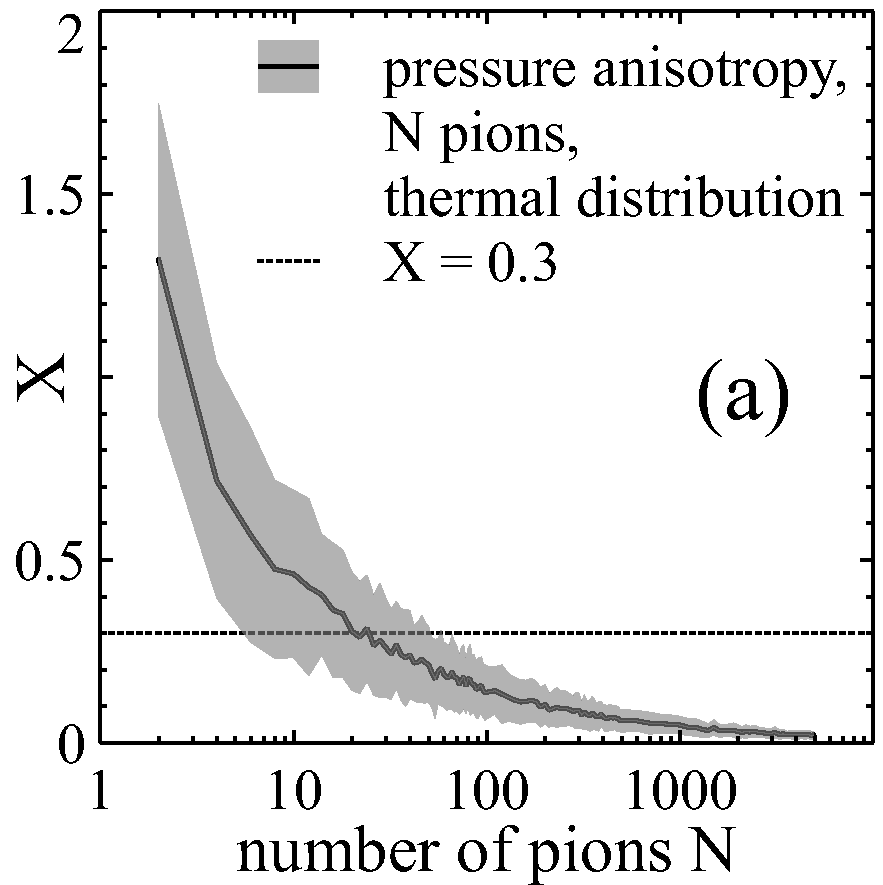
\includegraphics[width = 0.49\textwidth]{plots/thermalization_urqmd/x_pure_stat.pdf}
  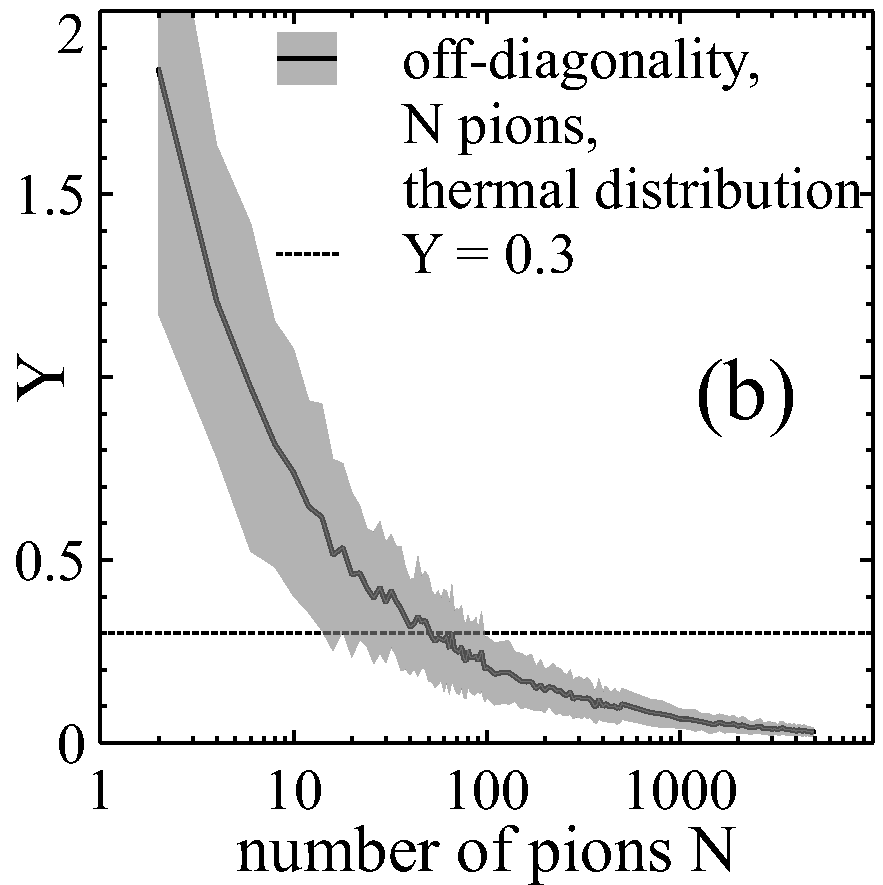
\includegraphics[width = 0.49\textwidth]{plots/thermalization_urqmd/y_pure_stat.pdf}
  \caption{Pressure anisotropy $X$ (panel a) and off-diagonality $Y$ (panel b)
  of $\Tmn$ for particles sampled according to thermal distributions. The effect
  of statistics on the deviation of energy-momentum tensor from the ideal fluid
  one is demonstrated.}
  \label{FIG:pure_stat_effect}
\end{figure}

This creates practical limitations for determining the ''true'' $\Tmn$ in
simulations: decreasing $\sigma$ by a factor of 10 demands increasing the statistics
by a factor of 1000! Also see regions with lower density are more demanding
with respect to statistics. To get some insights into the effect of statistics, 
an auxiliary simulation is performed: $N$ pions are generated, their momenta being
sampled from a thermal distribution with an ad-hoc temperature of $T = 0.2$ GeV,
then $\sum \frac{p^{\mu} p^{\mu}}{p^0}$ is computed, pressure isotropy $X$ and
off-diagonality $Y$ of the energy-momentum tensor from Eq. (\ref{cond_to_check})
are calculated. The number of pions $N$ was varied and $X$ and $Y$ are plotted versus
$N$. The results can be seen in Fig. \ref{FIG:pure_stat_effect}. For every point
the simulation was repeated 100 times and the standard deviation is displayed as
an error. For the thermal distribution $X=Y=0$ in the limit of $N\to \infty$, so
Fig. \ref{FIG:pure_stat_effect} demonstrates a pure effect of sampling a finite
number of particles.

Fig. \ref{FIG:pure_stat_effect} can be used to specify the number of events
needed to reach a good enough approximation to the ''true'' $\Tmn$. For example,
for $Y=0.3$ as an acceptable level, the condition of Eqn.
\ref{Eq:true_Tmn_condition} becomes $N_{ev} \rho \sigma^3 > 100$. From Fig.
\ref{FIG:pure_stat_effect} one can also see that the off-diagonality $Y$ is more
sensitive to statistics than the pressure isotropy $X$.

In the previous paragraph the effect of statistics itself was considered rather
as an obstacle to get the physical ''true'' $\Tmn$. However, recently
event-by-event simulations gained popularity, where the initial state for
hydrodynamics is intentionally constructed from a small number of events to
include the fluctuations. Let us see, how the number of events influences
deviations of $\Tmn$ from the ideal form in heavy ion collisions. The $\Tmn$ was
computed locally on every point of the grid, and as a general characteristic
the percentage of the event-plane area is chosen, where $X < 0.3$ ($Y < 0.3$). To
define the total area numerically, only grid cells, where pressure $p > 10^{-4}$
GeV/fm$^3$ are taken into account. For this example Au+Au collisions at $E =
80\emph{A}$ GeV with the impact parameter $b = 6$ fm are considered. The
smearing parameter $\sigma$ is 0.8 fm. Results are depicted in
Fig.~\ref{FIG:sensitivity_Nev}.

\begin{figure}
  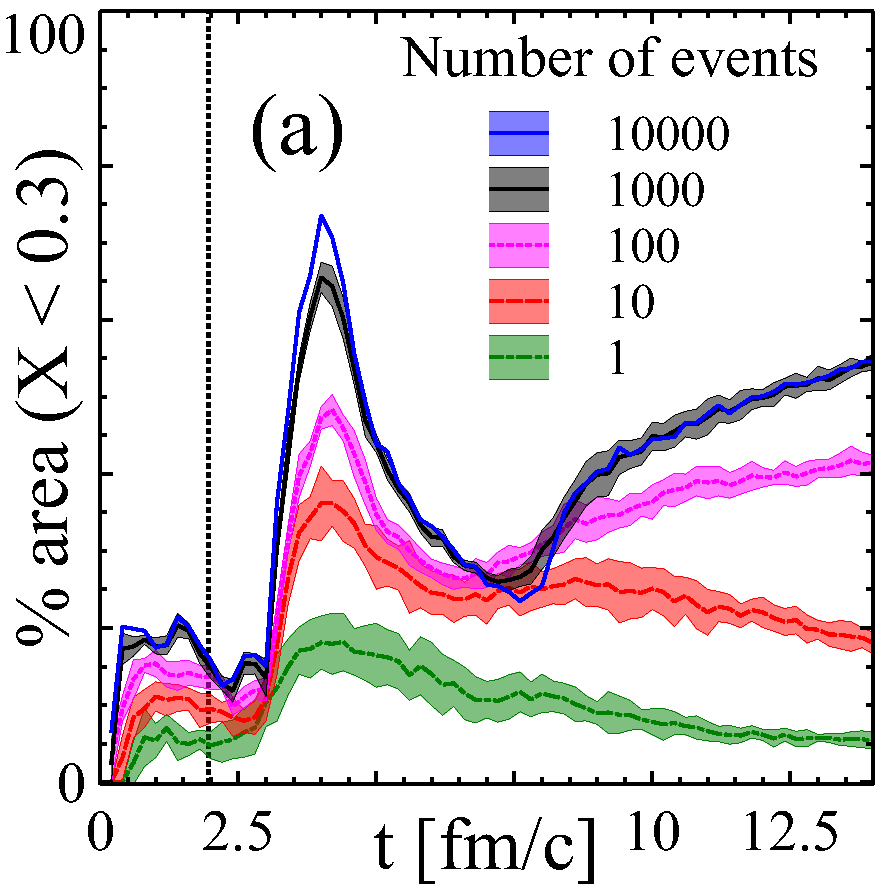
\includegraphics[width = 0.49\textwidth]{plots/thermalization_urqmd/E80_b6_x_area_Nev_dep.pdf}
  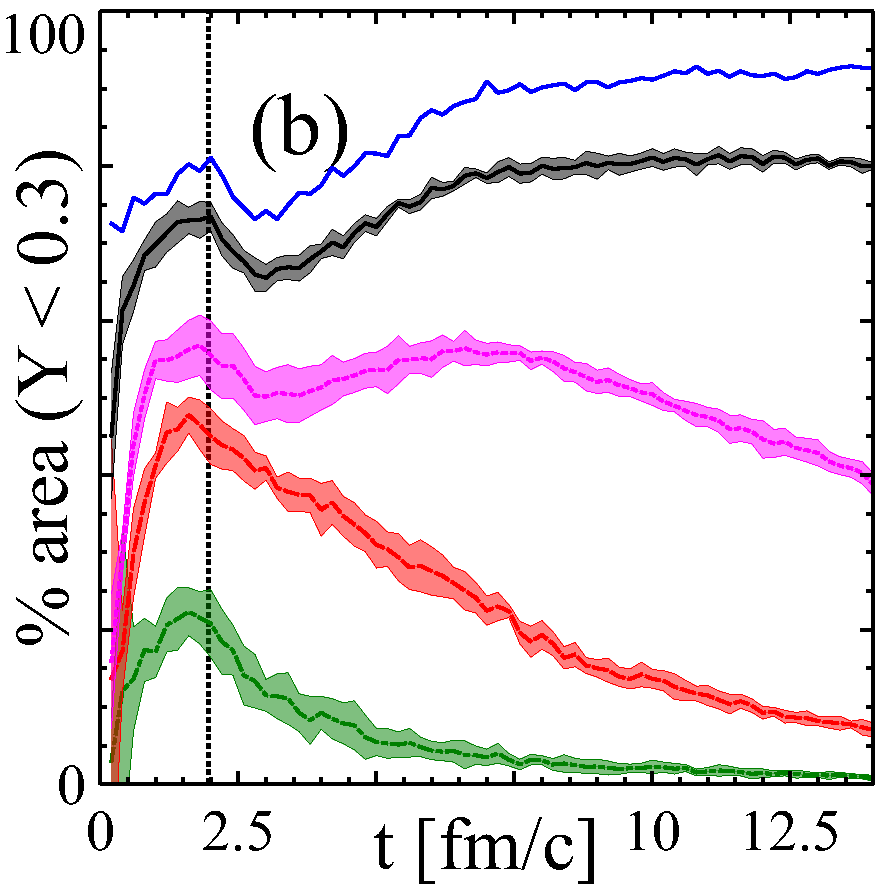
\includegraphics[width = 0.49\textwidth]{plots/thermalization_urqmd/E80_b6_y_area_Nev_dep.pdf}
  \caption{Event plane area percentage, where the pressure isotropy $X$ (panel a) or
           off-diagonality $Y$ (panel b) does not exceed 0.3 versus time for different
           number of events $N_{ev}$ used to construct $\Tmn$. Number of events
           $N_{ev} = 1$ corresponds to the event-by event case. The dotted line marks
           the geometrical overlap time.}
  \label{FIG:sensitivity_Nev}
\end{figure}

\begin{figure}
  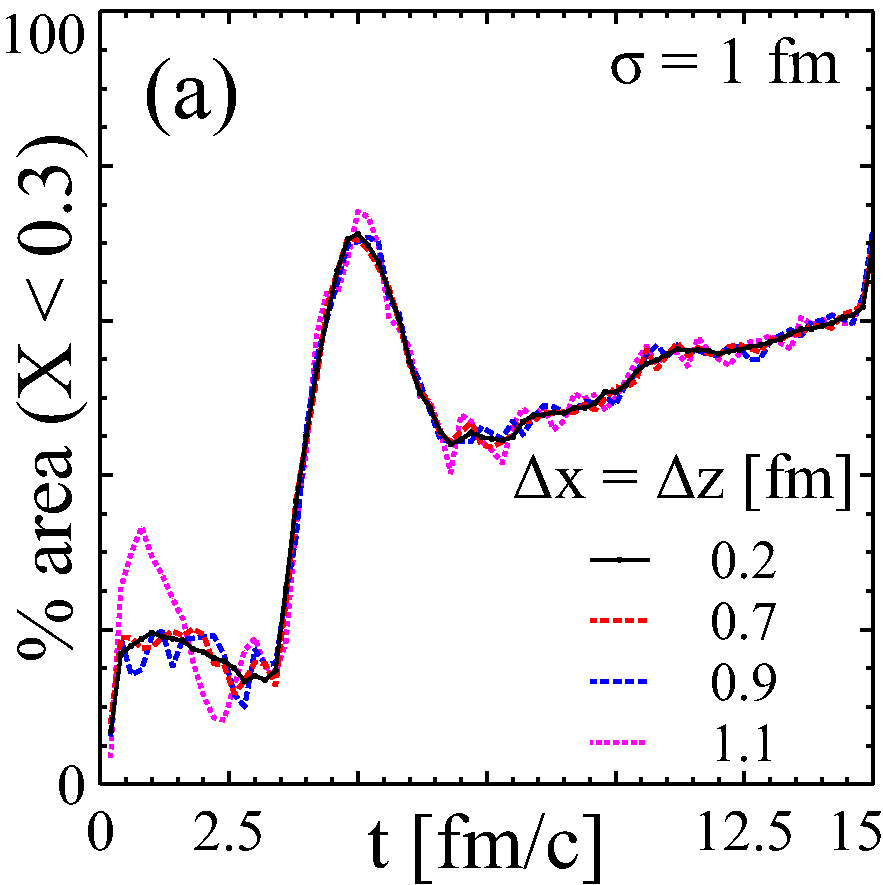
\includegraphics[width = 0.49\textwidth]{plots/thermalization_urqmd/grid_size_sensitivity.pdf}
  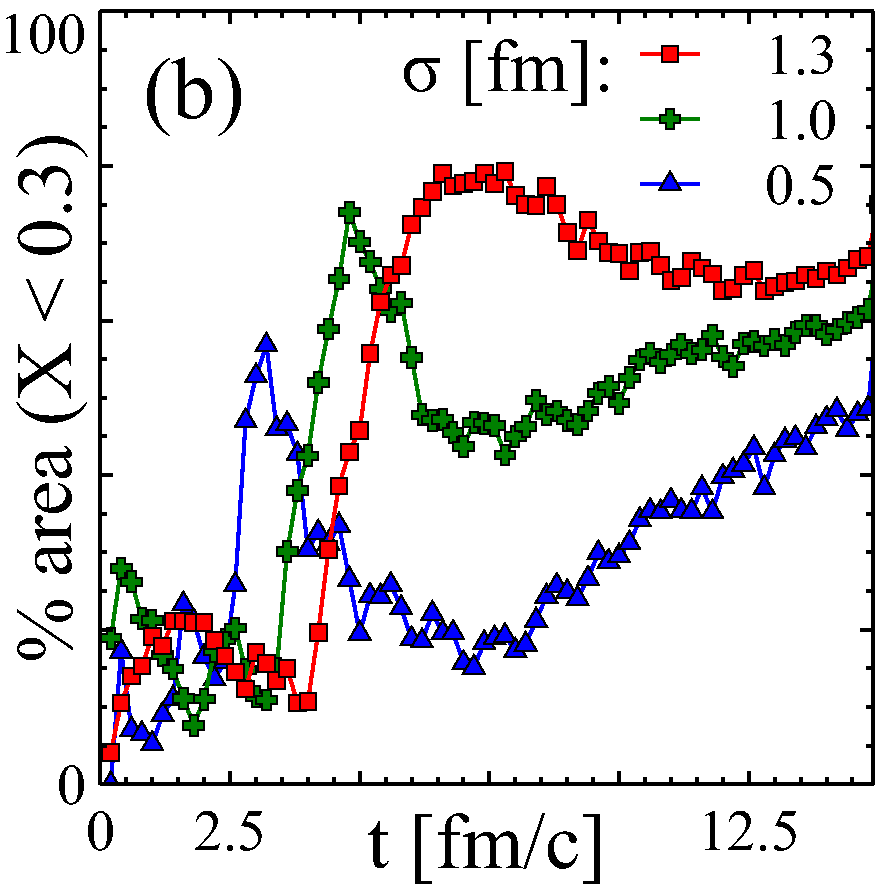
\includegraphics[width = 0.49\textwidth]{plots/thermalization_urqmd/sigma_sensitivity.pdf}
  \caption{Event plane area percentage, where pressure isotropy $X$ does not
           exceed 0.3. Au+Au versus time. $E = 80\emph{A}$ GeV, centrality $b = 6$ fm,
           number of events $N_{ev} = 1000$. Gaussian smearing $\sigma$ (right) and grid
           spacing $\Delta x = \Delta z$ (left) are varied to study sensitivity of results
           to them.}
  \label{FIG:sensitivity_sigma_dx}
\end{figure}

One can see that for this given $\sigma$ 1000 events are enough for $X$ to
saturate, so the line for $N_{ev} = 1000$ represents results for the physical
pressure isotropy, i.e. due to deviation of $\mathit{f}(\vec{r},\vec{p})$ in the
transport from equilibrium. For $Y$ at $N_{ev} = 10000$ almost all the event
area has small off-diagonality, which means that the physical off-diagonality is
small. For event-by-event simulations deviations of $\Tmn$ from ideal fluid are
dominated by statistical effects.

In addition to the effect of statistics the effect of other nuisance parameters
was investigated, i.e. the grid spacing and the Gaussian smearing. According to
Fig.~\ref{FIG:sensitivity_sigma_dx}, the grid spacing does not influence the
results, if taken sufficiently small. This is expected, because the grid does
not participate in the simulation or in the calculation of $\Tmn$, it only
determines the resolution of the $\Tmn$ output. The only effect of the grid spacing
is on the precision of the area calculation by counting cells, here the resolution
of the output matters. At early times, it makes some difference, because the
total area is small. That is why in the following $\Delta x = \Delta z = 0.6$
fm was chosen. At the same time the Gaussian width $\sigma$ influences the results very
significantly, as it can be seen from Fig.~\ref{FIG:sensitivity_sigma_dx}. The
effect of $\sigma$ is twofold: on the one hand a larger $\sigma$ means
effective increase of statistics. On the other hand, if the pressure anisotropy
is large at some space point due to physics, the Gaussian smearing will spread
this asymmetry in a 1-2 $\sigma$ radius.

\begin{figure}
  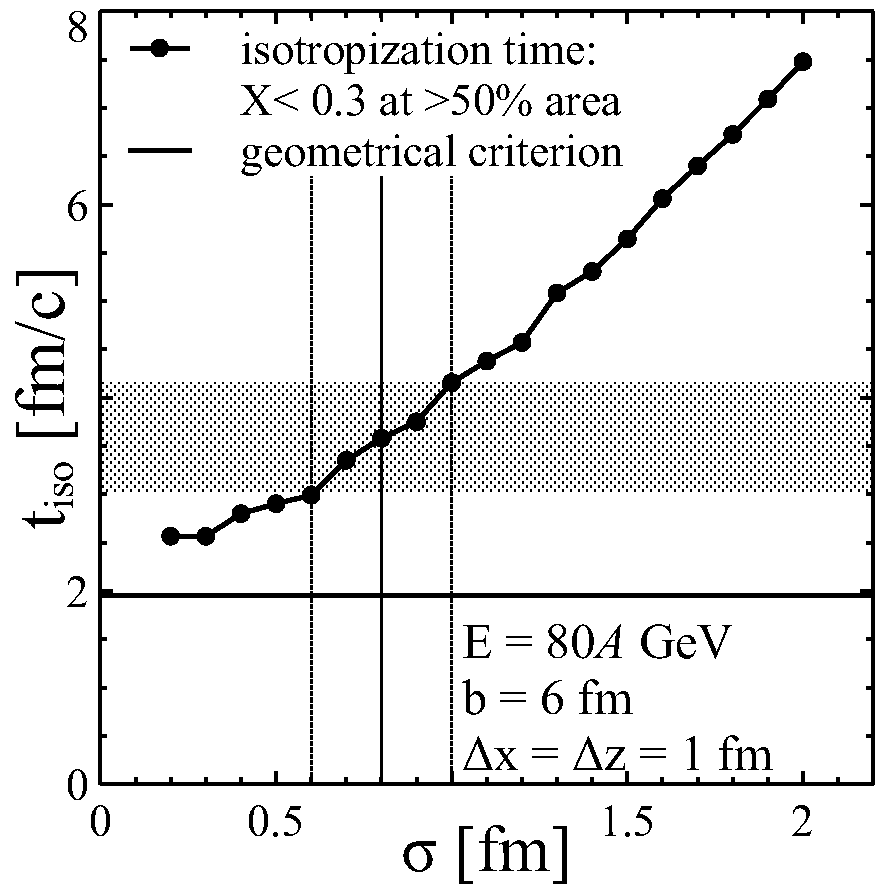
\includegraphics[height = 9cm]{plots/thermalization_urqmd/t_iso_vs_sigma.pdf}
  \caption{Isotropization time (such time that more than 50\% of event plane
           area have pressure isotropy $X < 0.3$) versus $\sigma$.}
  \label{FIG:t_iso_sensitivity_sigma}
\end{figure}

To characterize the influence of $\sigma$ in a simpler way, $t_{iso}$ versus
$\sigma$ was plotted, where $t_{iso}$ is the earliest time when at least 50\%
of the area have $X < 0.3$. Let us refer to this time as \emph{isotropization time}
as it is further described in the following Section. In
Fig.~\ref{FIG:t_iso_sensitivity_sigma} this dependence is displayed, the
isotropization time is monotonously growing with $\sigma$ and is approaching
the geometrical time for~$\sigma \to 0$. Taking the limit $\sigma \to 0$ is
computationally challenging, because one has to increase statistics as
$\sigma^{-3}$, as shown previously. Instead a reasonable value $\sigma = 0.8$
fm was chosen and systematic errors were assigned to our results, corresponding
to changing $\sigma$ in the range $(0.6-1.0)$ fm. Another justification for
this treatment is that none of the existing models attempts to consider the
''physical'' limit of $\sigma \to 0,\, N_{ev} \rho \sigma^3 \to \infty$, all
the models use some fixed width instead.

\section{Results} \label{sec:Results}

\begin{figure*}
  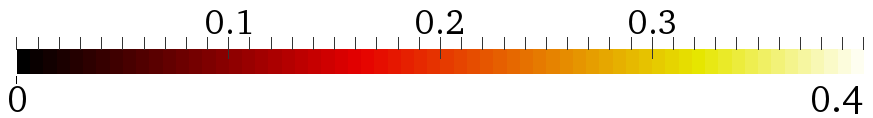
\includegraphics[height = 1cm]{plots/thermalization_urqmd/E80b6_x_paraview_color_legend.png} \\
  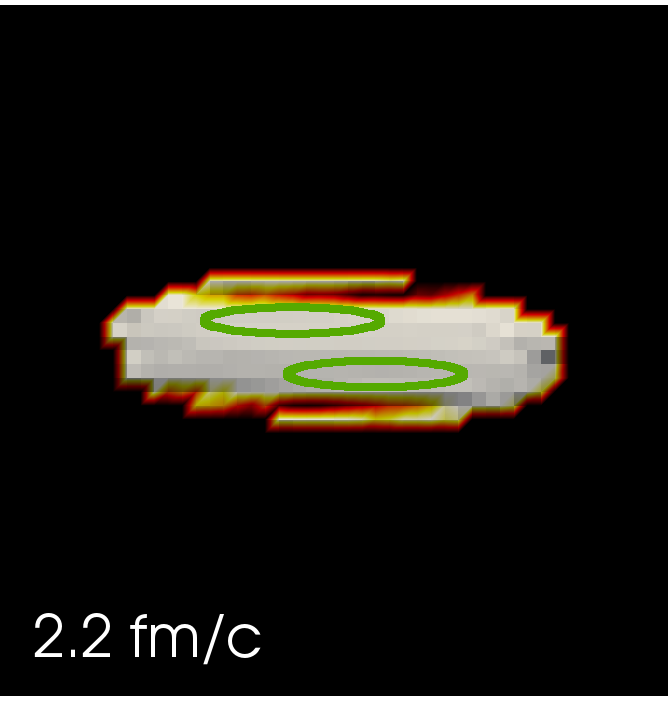
\includegraphics[width = 3.0cm]{plots/thermalization_urqmd/E80b6_x_paraview_t2_2fm.png}
  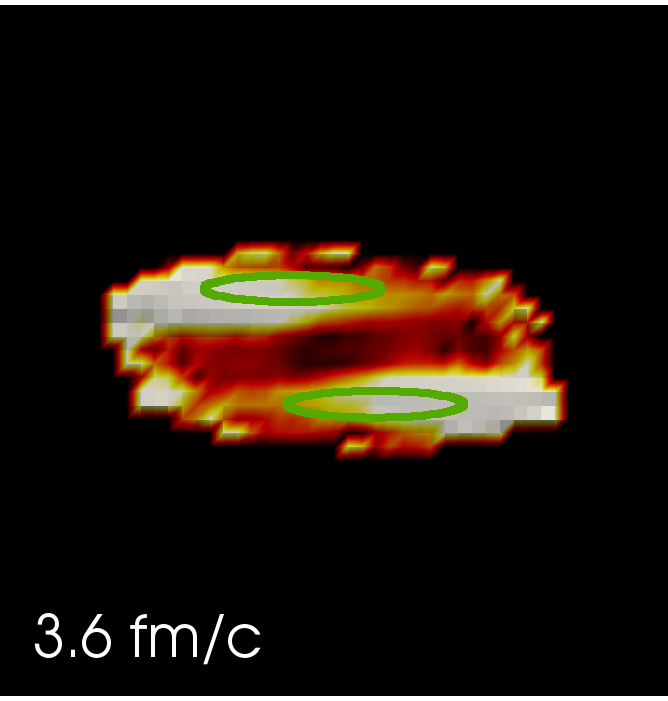
\includegraphics[width = 3.0cm]{plots/thermalization_urqmd/E80b6_x_paraview_t3_6fm.png}
  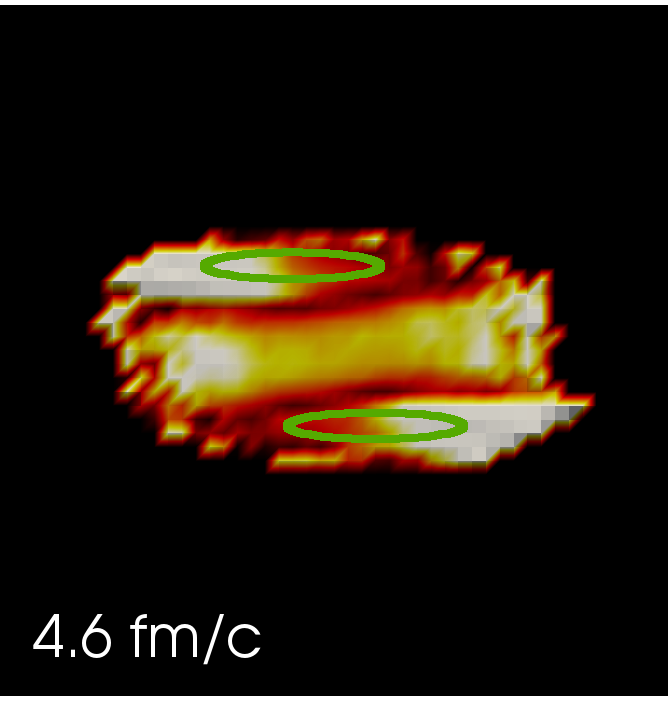
\includegraphics[width = 3.0cm]{plots/thermalization_urqmd/E80b6_x_paraview_t4_6fm.png}
  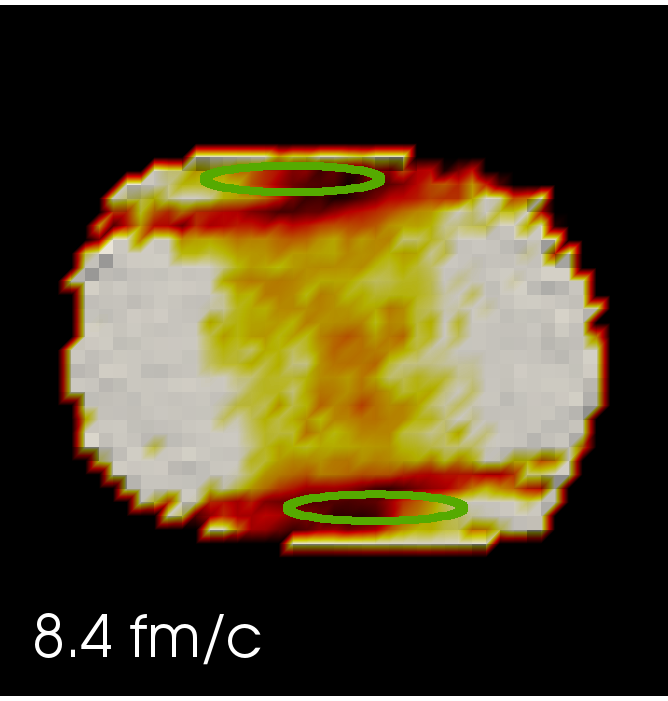
\includegraphics[width = 3.0cm]{plots/thermalization_urqmd/E80b6_x_paraview_t8_4fm.png}
  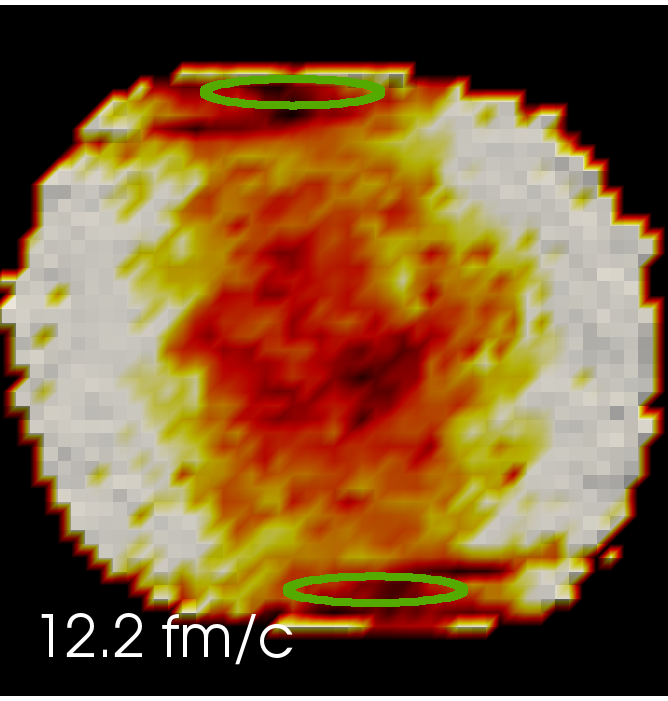
\includegraphics[width = 3.0cm]{plots/thermalization_urqmd/E80b6_x_paraview_t12_2fm.png}
  \caption{Space-time evolution of the pressure anisotropy $X =
           \frac{|T_L^{11}-T_L^{22}|+|T_L^{22}-T_L^{33}|+|T_L^{33}-T_L^{11}|}
           {T_L^{11}+T_L^{22}+T_L^{33}}$
           (see color scale above the Fig.) for collision energy
           $\Elab = 80$ \emph{A} GeV and impact parameter $b = 6$ fm.
           If the value of $X$ exceeds color map maximum, it is marked with the same
           color as maximum. Solid lines mark the positions of the nuclei, if they
           would not interact.}
  \label{FIG:x_paraview_space_time_evolution}
\end{figure*}

While in the previous section the effects of nuisance parameters on
the energy-momentum tensor generated from particles were studied, here the
dependence on physical parameters is considered, namely collision energy and centrality.
All the following figures are shown for grid spacing $\Delta x = \Delta z = 0.6$ fm,
Gaussian smearing $\sigma = 0.8$ fm, and number of events $N_{ev} = 1000$.
The smearing kernel is defined as in section \ref{sec:final_coarse_graining}.

\subsection{Pressure anisotropy}

\begin{figure}
  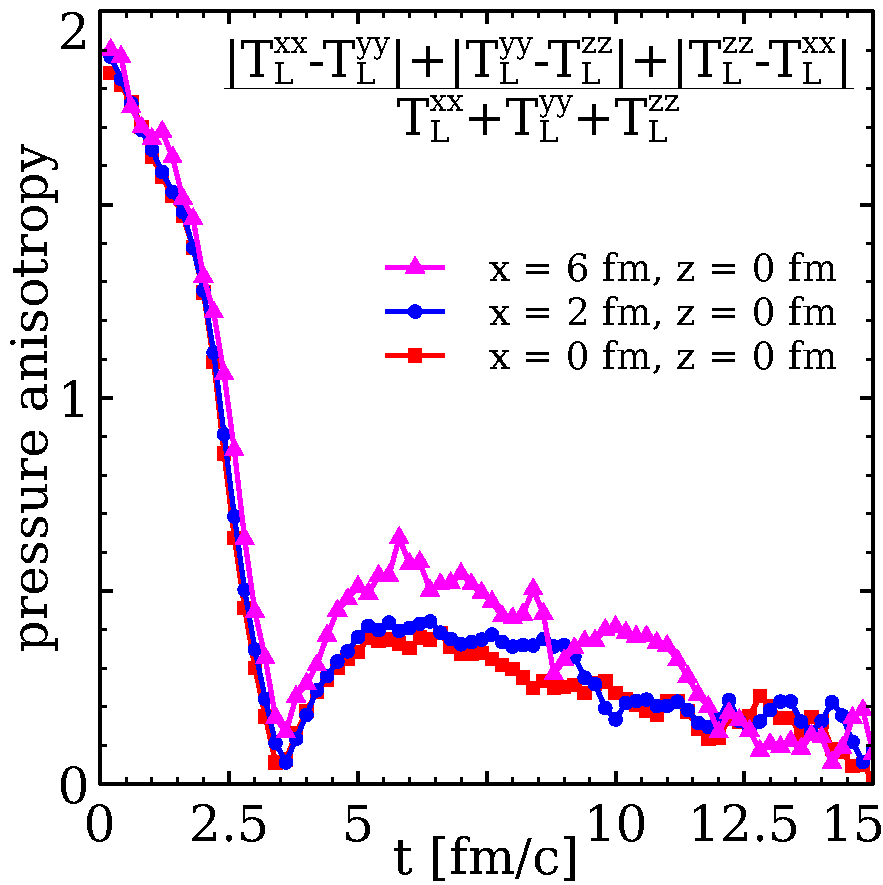
\includegraphics[width = 7cm]{plots/thermalization_urqmd/E80b6_x_vs_t_few_space_points.pdf}
  \caption{Example for the behaviour of the pressure anisotropy versus time in Au+Au
           collisions at $\Elab = 80$ \emph{A} GeV and impact parameter $b = 6$ fm.}
  \label{FIG:x_vs_t_few_space_points}
\end{figure}

The pressure anisotropy $X$ satisfies the following properties: $X \le 2$ for
any tensor and $X = 0$, if and only if $T^{11}_L = T^{22}_L = T^{33}_L$ as it is
for an ideal fluid. For viscous hydrodynamics it is necessary that $X \ll
1$. Here $X_{crit} = 0.3$ is considered as a limiting value, when viscous
hydrodynamics is still applicable. Changing $X_{crit}$ to 0.4 leaves one with
qualitatively the same results and conclusions. Fig.
\ref{FIG:x_paraview_space_time_evolution} gives a qualitative impression of the
space-time evolution of the pressure anisotropy. Even though the figure shows a
particular energy of $\Elab = 80\emph{A}$ GeV and centrality $b = 6$ fm, some
features are universal for all energies and centralities that were considered:

\begin{itemize}
  \item On the borders of the expanding system the anisotropy is always high,
        thus these regions are never consistent with viscous hydrodynamics.
  \item After some moment of time a relatively isotropized central region
        rapidly expands and never disappears completely during the time evolution
\end{itemize}

To make quantitative statements let us consider the evolution of the pressure
anisotropy at several points along the x axis (z = 0) versus time. This is shown
in Fig.~\ref{FIG:x_vs_t_few_space_points}. One can see that in the beginning the
anisotropy is almost maximal, then it rapidly decreases and never rises too much
again. As shown in the previous section, $N_{ev} = 1000$ is enough to
suppress the anisotropy due to statistics, so the behaviour of $X$ in
Fig.~\ref{FIG:x_vs_t_few_space_points} is dominated by physics. However, the
impact of statistical fluctuations can be observed already at $t > 5$ fm/c: $X$
starts to fluctuate in space and time. One can see this both in
Fig.~\ref{FIG:x_paraview_space_time_evolution} at later times and in
Fig.~\ref{FIG:x_vs_t_few_space_points}.

\begin{figure}
  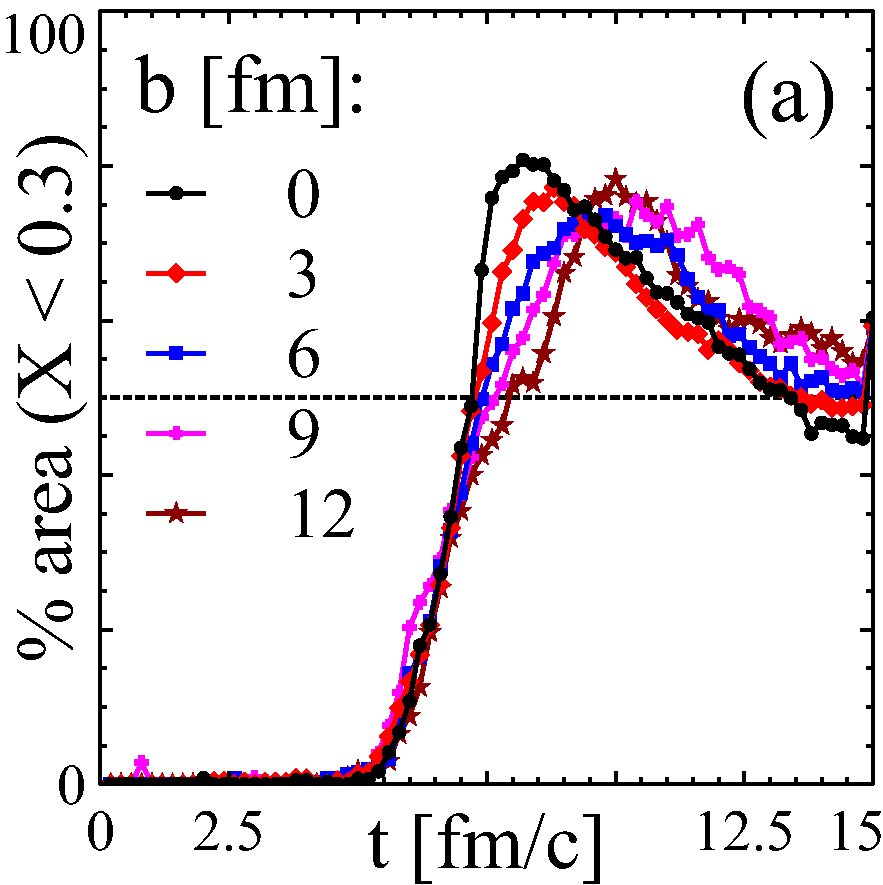
\includegraphics[width = 0.32\textwidth]{plots/thermalization_urqmd/plot_x_area_percentages_E5.pdf}
  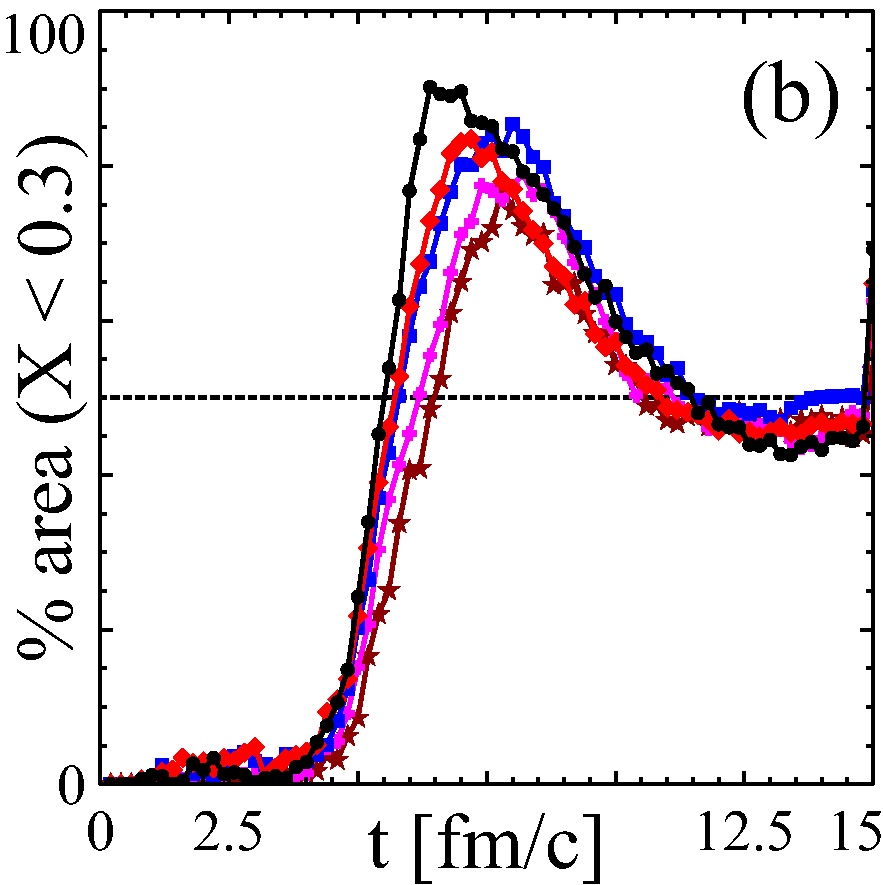
\includegraphics[width = 0.32\textwidth]{plots/thermalization_urqmd/plot_x_area_percentages_E10.pdf}
  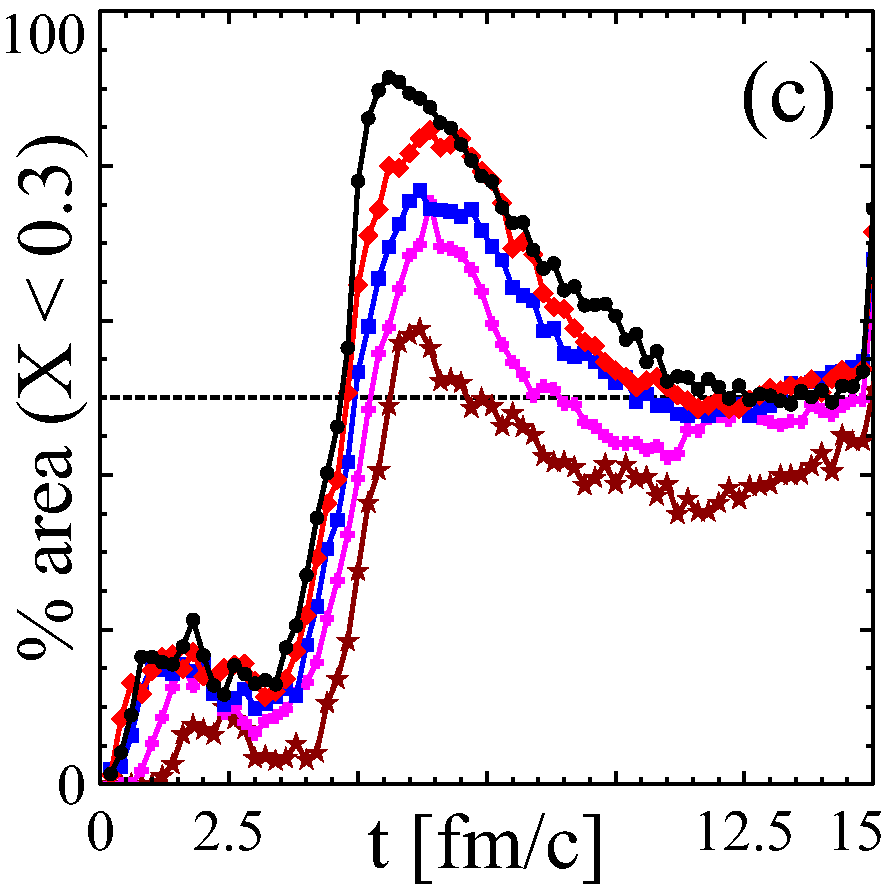
\includegraphics[width = 0.32\textwidth]{plots/thermalization_urqmd/plot_x_area_percentages_E20.pdf}\\
  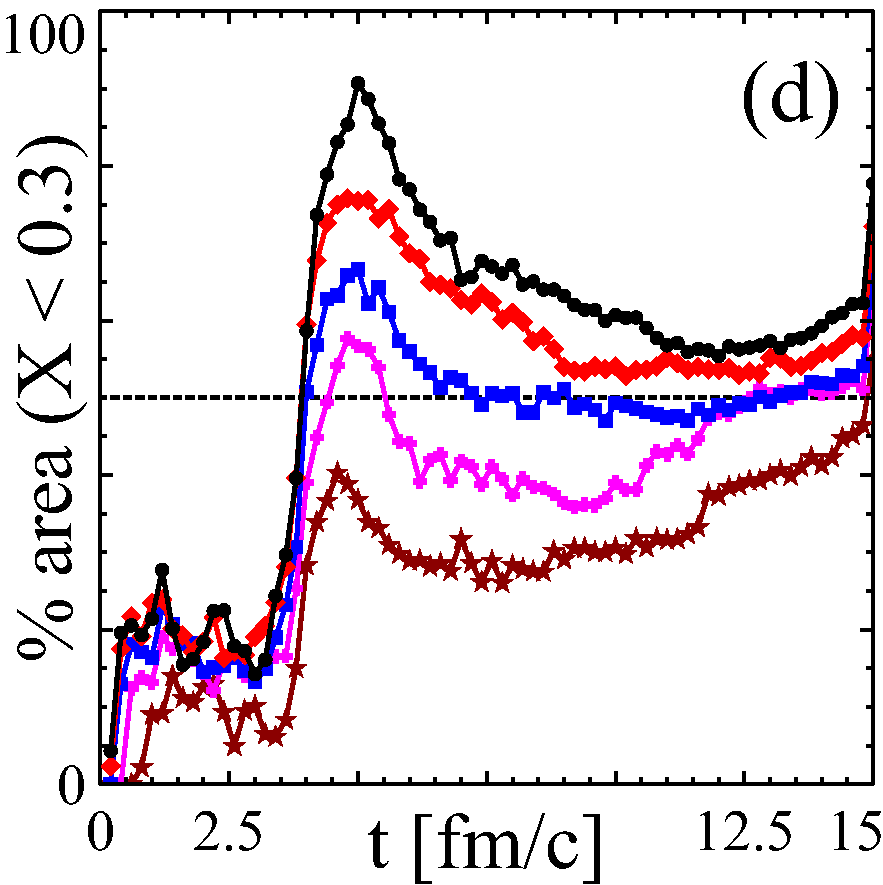
\includegraphics[width = 0.32\textwidth]{plots/thermalization_urqmd/plot_x_area_percentages_E40.pdf} 
  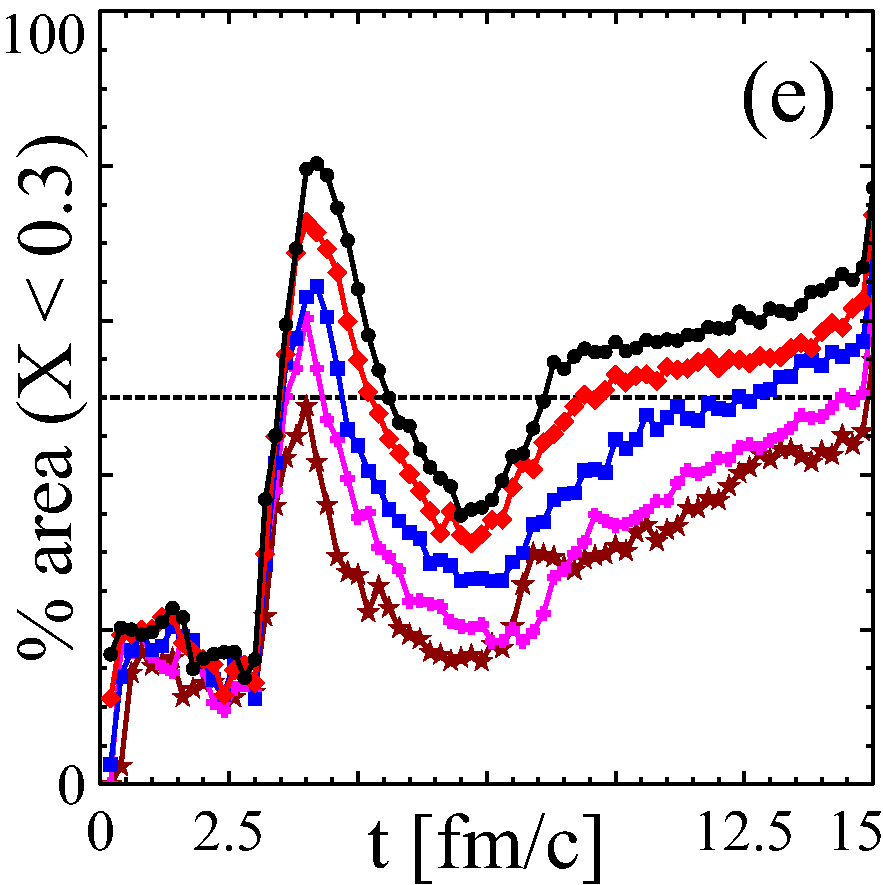
\includegraphics[width = 0.32\textwidth]{plots/thermalization_urqmd/plot_x_area_percentages_E80.pdf}
  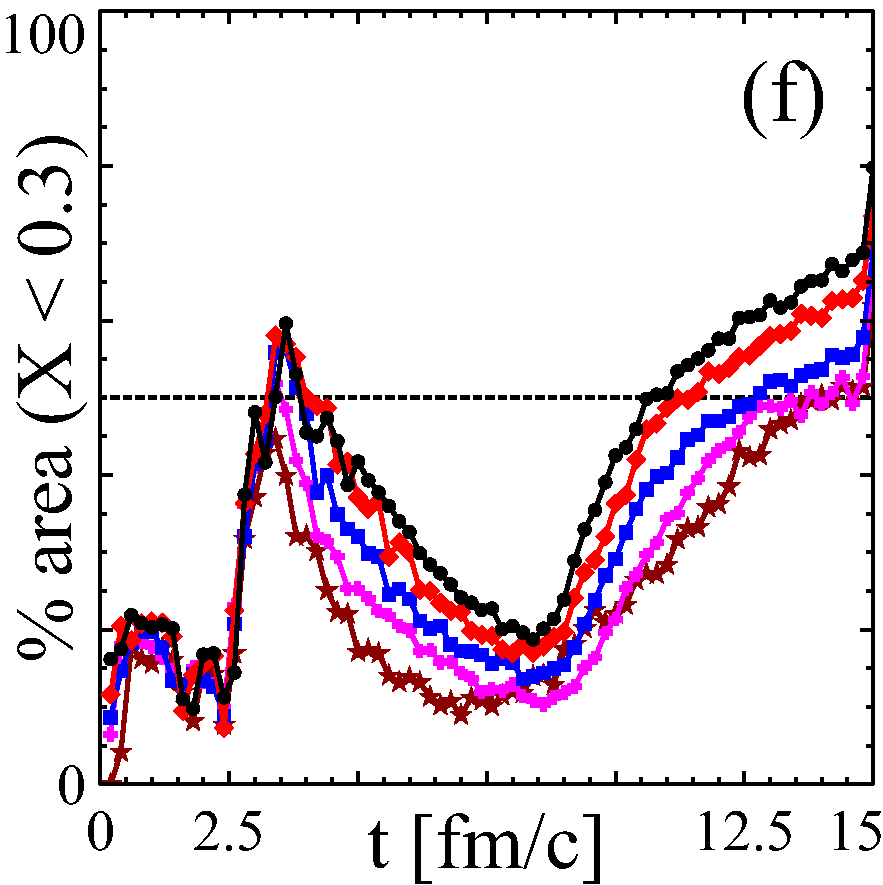
\includegraphics[width = 0.32\textwidth]{plots/thermalization_urqmd/plot_x_area_percentages_E160.pdf}
  \caption{Percentage of area in the event plane, where pressure anisotropy $X <
           0.3$, for Au+Au collision energies $\Elab = 5$, $10$, $20$, $40$, $80$,
           $160$ \emph{A} GeV (panels (a) - (f) correspondingly).}
  \label{FIG:x_area_percentages}
\end{figure}

After looking at the space-time evolution of the anisotropy in 2D as in
Fig.~\ref{FIG:x_paraview_space_time_evolution} for different energies, one gets
the impression that there is a special moment $t_{iso}$ for each energy and
centrality, before which pressures are highly anisotropic in the whole event
plane and after which there emerges a considerable isotropic region. To quantify
this feeling let us consider the ratio of the area, where $X < 0.3$ to the total area
versus time. From Fig.~\ref{FIG:x_area_percentages} one can see that there is
indeed a steep rise of the isotropized area at some point in time for every considered
energy and centrality. Let us define the \emph{isotropization time} $t_{iso}$
such that more than 50\% of the area has $X < 0.3$ at $t = t_{iso}$. The
behaviour of this isotropization time versus energy and centrality is compared
to the geometrical criterion in Fig.~\ref{FIG:t_x_energy}. One can see that the
isotropization time decreases with energy, but remains larger than the
geometrical criterion for all energies except $5\emph{A}$~GeV. It is interesting
to note that the isotropization time differs with centrality: for larger impact
parameters $b$ it slightly increases. One might assume that this has a pure
geometrical reason: $t_0 = 0$ is chosen in UrQMD as a moment when nuclei touch
each other in a central collision. However, for peripheral collisions the nuclei
will only touch at $t_0(b) = \frac{R}{\gamma v} (1 - \sqrt{1 - (b/2R)^2})$. In
Fig.~\ref{FIG:t_x_b} one can see that this naive expectation yields the right
trend: $t_{iso}$ rises with centrality and the rise is smaller for higher
energies. However, quantitatively it overestimates $t_{iso}$ for large impact
parameters.

\begin{figure}
  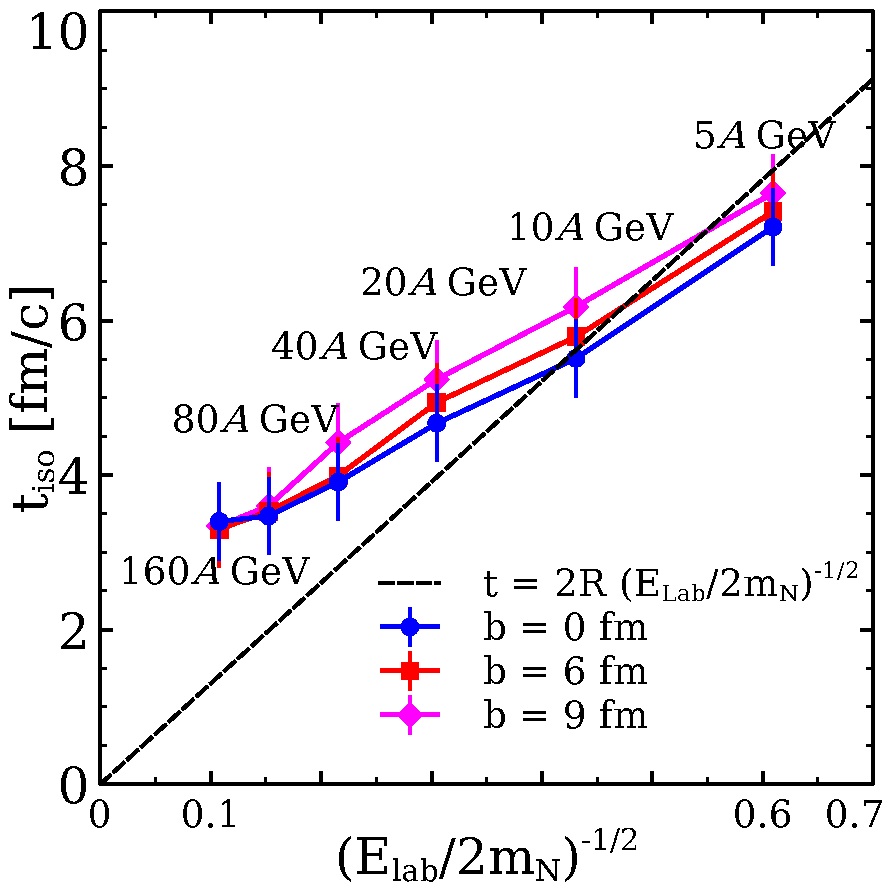
\includegraphics[width = 0.6\textwidth]{plots/thermalization_urqmd/t_x_vs_energy.pdf}
  \caption{Isotropization time $t_{iso}$ (see definition in the text) versus energy and centrality.}
  \label{FIG:t_x_energy}
\end{figure}

Let us compare the above findings to the study by Bravina et al.
\cite{Bravina:2008ra}, where one central cell of $(5 \times 5 \times 5)$ fm$^3$
was chosen to study the pressure anisotropy of the energy-momentum tensor in
Au+Au collisions. An isotropization time was  defined, and it did not change
significantly after zooming into the central cell to $(1 \times 1 \times 1)$ fm$^3$.
This allowed for the conclusion that isotropization happens rapidly in a large
volume. The isotropization time determined in this study also decreases with
collision energy. All of these results are confirmed in the present study.
However, our isotropization times are smaller than the ones obtained by Bravina
et al. There are two possible reasons for that.  First, the criterion for
isotropization used here is less strict: while here at least 50\% of
event plane area to have $X < 0.3$ is required, the central cell study demands
$p_z/p_x - 1 < 0.1$ in the whole cell, which corresponds to $X < 0.065$. Secondly,
here only the deviation of the energy-momentum tensor from equilibrium is considered,
but in the study \cite{Bravina:2008ra} also deviations of hadron multiplicities from
equilibrium are taken into account.

\begin{figure}
  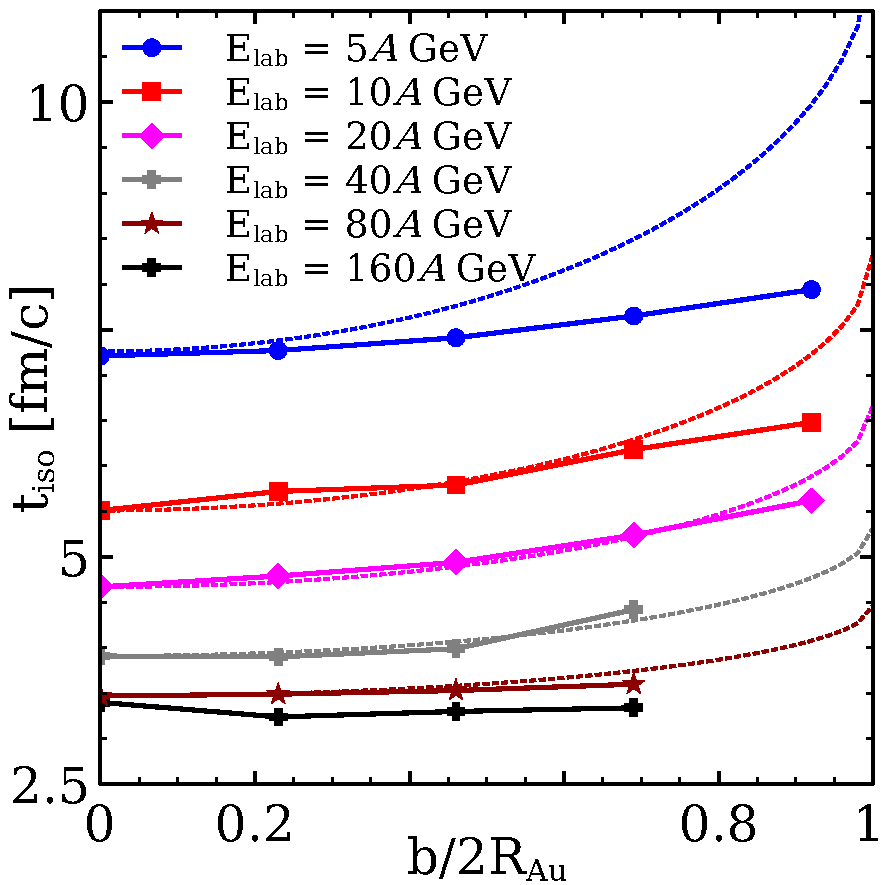
\includegraphics[width = 0.6\textwidth]{plots/thermalization_urqmd/t_x_vs_b.pdf}
  \caption{Isotropization time $t_{iso}$ (see definition in the text) versus
           centrality. The dotted lines represent the naive expectation from the
           collision geometry: $t_{iso}(b) = t_{iso}(b = 0) +
           \frac{R}{\gamma v} (1 - \sqrt{1 - (b/2R)^2})$.}
  \label{FIG:t_x_b}
\end{figure}

\subsection{Off-diagonality of $\Tmn$ in the local rest frame}

\begin{figure*}
  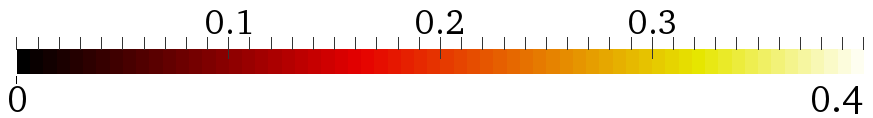
\includegraphics[height = 1cm]{plots/thermalization_urqmd/E80b6_x_paraview_color_legend.png} \\
  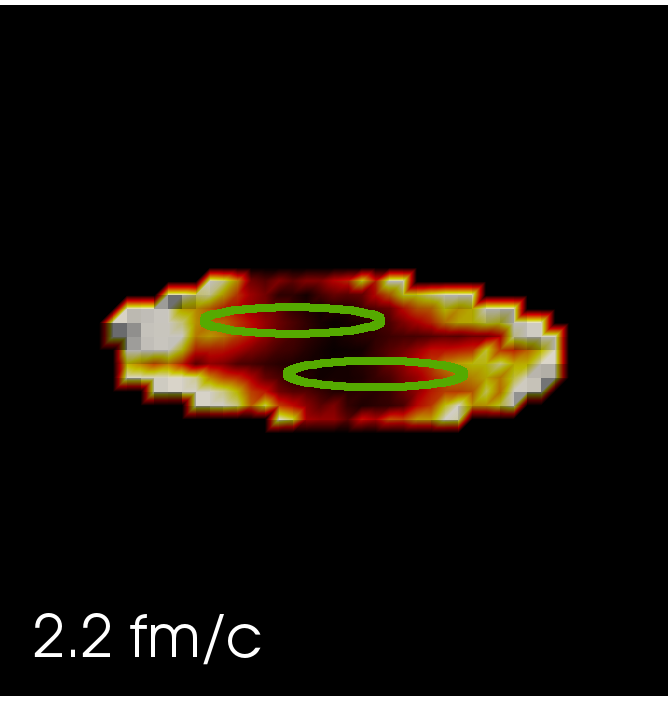
\includegraphics[width = 3.0cm]{plots/thermalization_urqmd/E80b6_y_paraview_t2_2fm.png}
  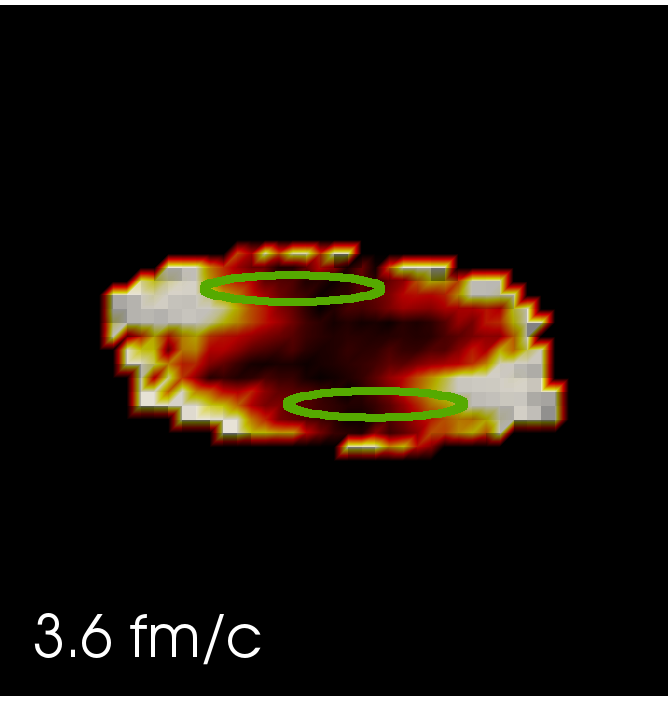
\includegraphics[width = 3.0cm]{plots/thermalization_urqmd/E80b6_y_paraview_t3_6fm.png}
  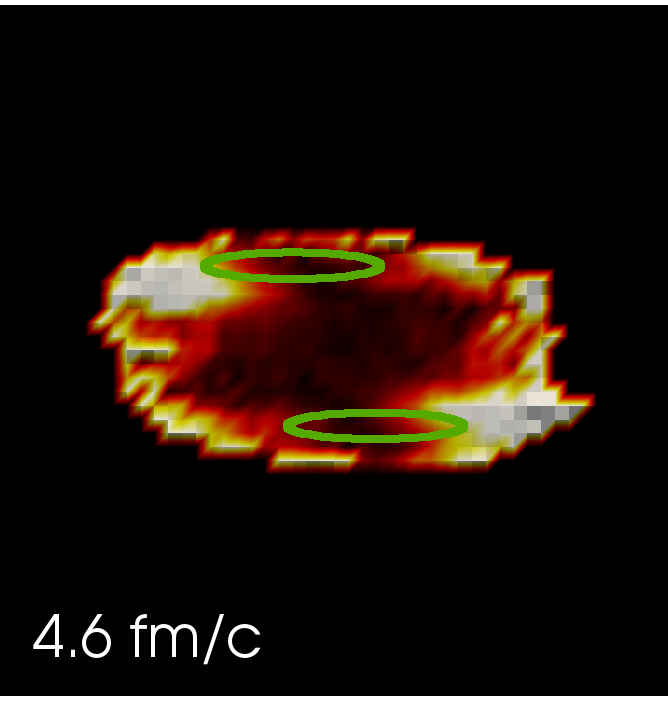
\includegraphics[width = 3.0cm]{plots/thermalization_urqmd/E80b6_y_paraview_t4_6fm.png}
  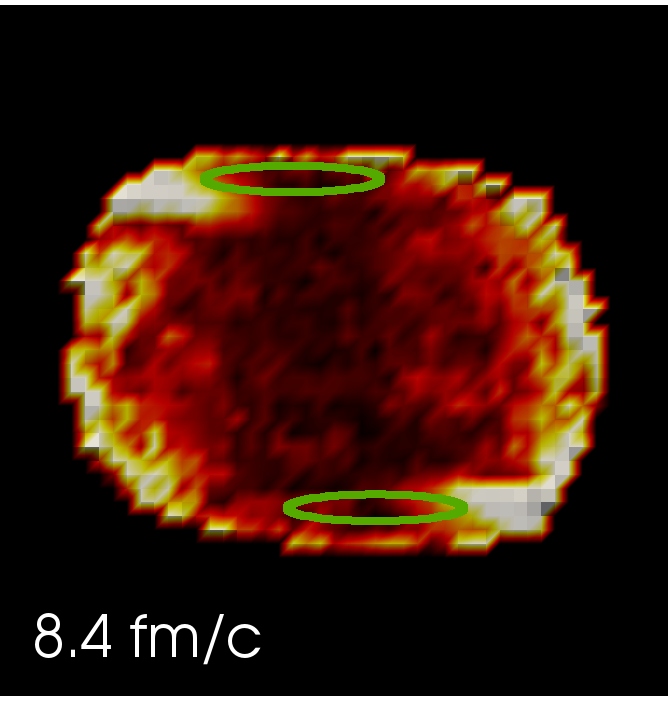
\includegraphics[width = 3.0cm]{plots/thermalization_urqmd/E80b6_y_paraview_t8_4fm.png}
  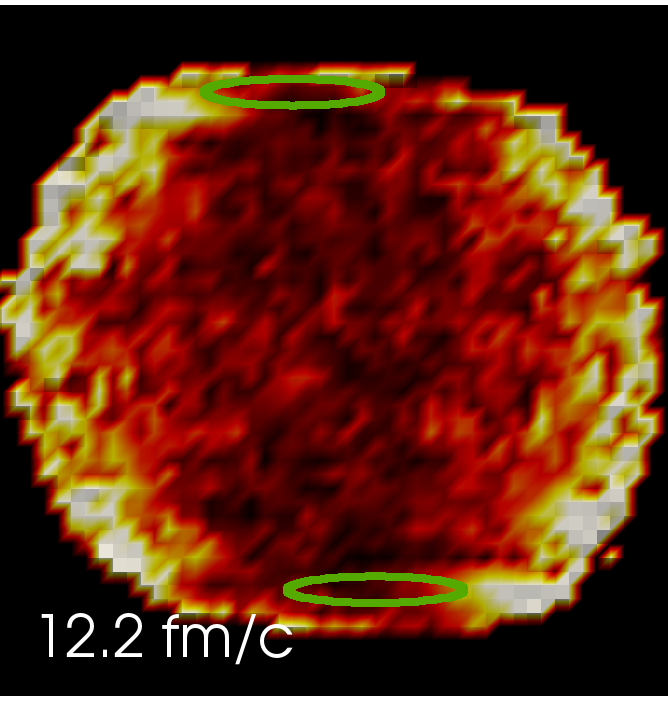
\includegraphics[width = 3.0cm]{plots/thermalization_urqmd/E80b6_y_paraview_t12_2fm.png}
  \caption{Space-time evolution of the off-diagonality $Y = \frac{3(|T^{12}_L| +
           |T^{23}_L| + |T^{13}_L|)}{T^{11}_L + T^{22}_L + T^{33}_L}$ (see color scale
           above the Fig.) for collision energy $\Elab = 80$ \emph{A} GeV and
           impact parameter $b = 6$ fm. If the value of $Y$ exceeds color map maximum,
           it is marked with the same color as maximum. Solid lines mark the positions
           of the nuclei, if they would not interact.}
  \label{FIG:y_paraview_space_time_evolution}
\end{figure*}

The off-diagonality $Y = \frac{3(|T^{12}_L| + |T^{23}_L| +
|T^{13}_L|)}{T^{11}_L + T^{22}_L + T^{33}_L}$ characterizes the size of the
off-diagonal components of the stress tensor compared to the pressure. In ideal
hydrodynamics $Y = 0$. For the applicability of viscous hydrodynamics it is
necessary that $Y \ll 1$. Here $Y_{crit} = 0.3$ is considered as a value, after which
viscous hydrodynamics is hardly applicable. An example for the space-time
evolution of $Y$ is given in Fig.~\ref{FIG:y_paraview_space_time_evolution}.
From this Fig. it can be seen that in the central region $Y$ is always small.
On the boundaries $Y$ is typically large due to statistical effects. A
quantitative study similar to the study of the pressure isotropy $X$ shows that
for all considered energies and centralities more than 80\% of the event plane
area have $Y < 0.3$ for the whole time of the evolution.

\subsection{Relative velocity between Landau and Eckart frames}


\begin{figure*}
  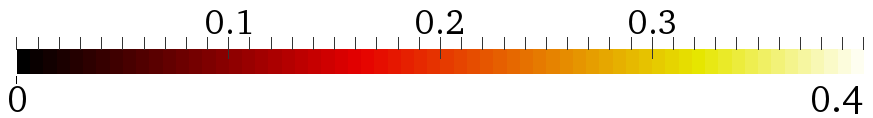
\includegraphics[height = 1cm]{plots/thermalization_urqmd/E80b6_x_paraview_color_legend.png} \\
  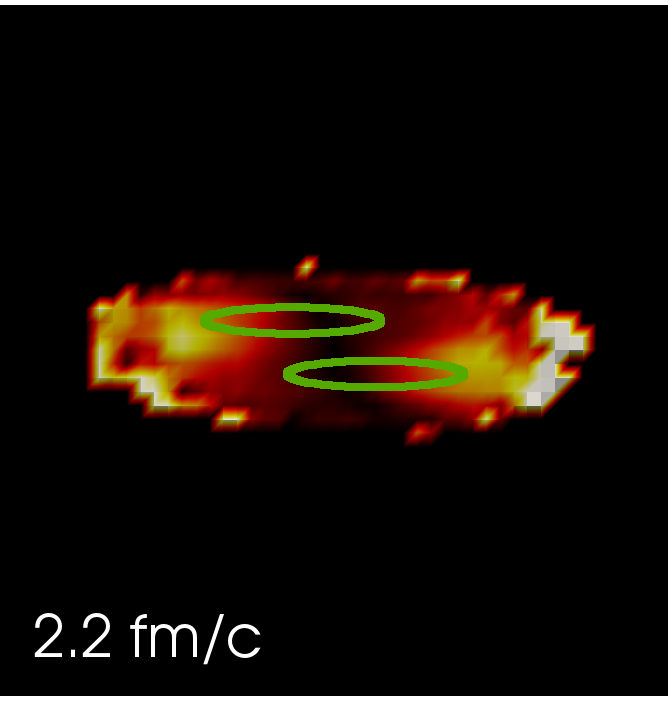
\includegraphics[width = 3.0cm]{plots/thermalization_urqmd/E80b6_vLE_paraview_t2_2fm.png}
  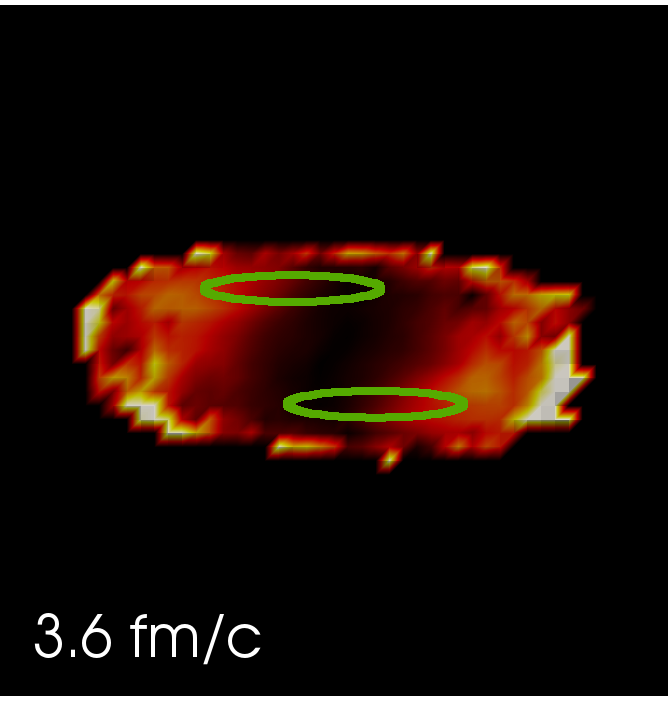
\includegraphics[width = 3.0cm]{plots/thermalization_urqmd/E80b6_vLE_paraview_t3_6fm.png}
  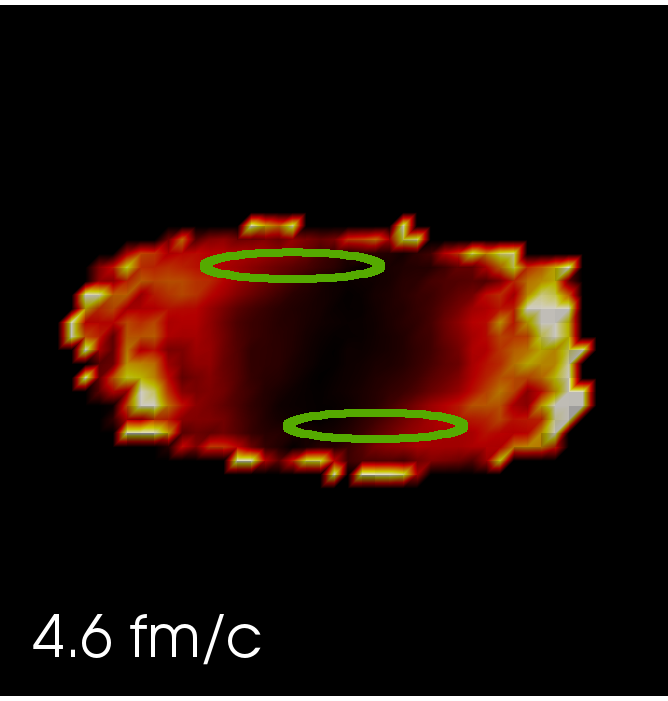
\includegraphics[width = 3.0cm]{plots/thermalization_urqmd/E80b6_vLE_paraview_t4_6fm.png}
  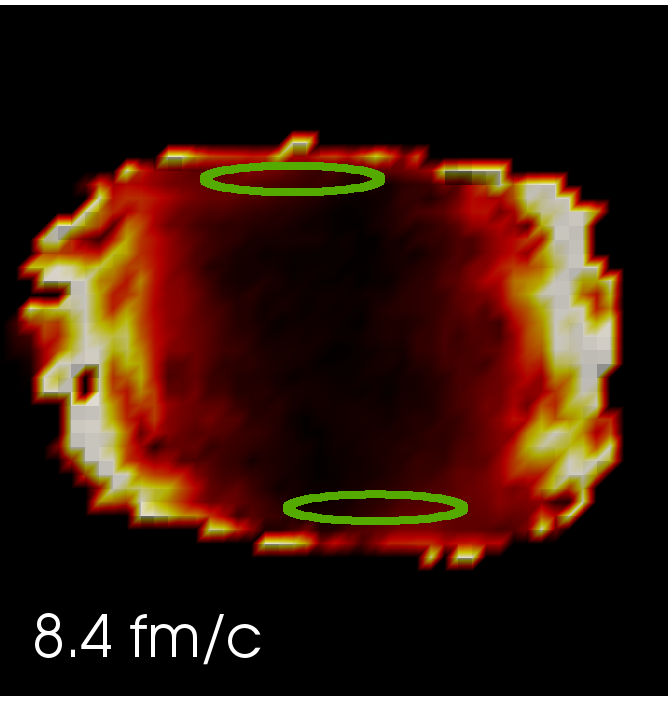
\includegraphics[width = 3.0cm]{plots/thermalization_urqmd/E80b6_vLE_paraview_t8_4fm.png}
  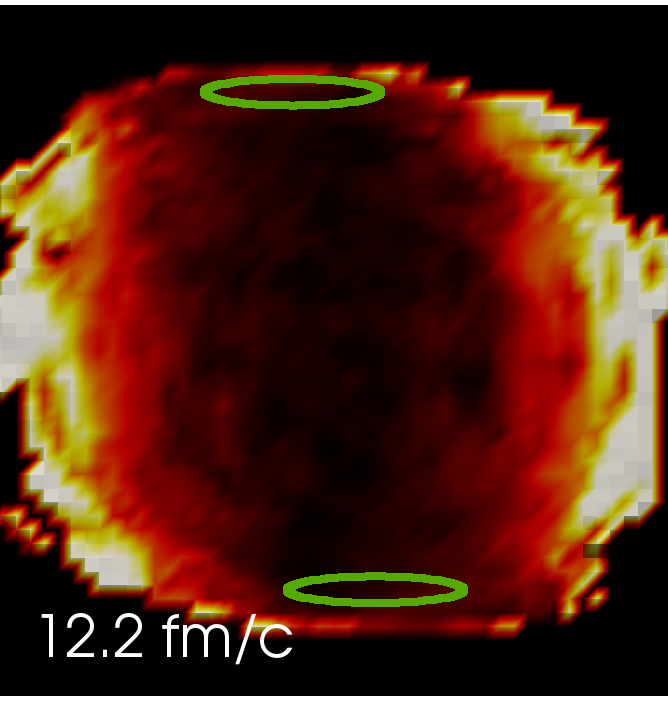
\includegraphics[width = 3.0cm]{plots/thermalization_urqmd/E80b6_vLE_paraview_t12_2fm.png}
  \caption{Space-time evolution of relative velocity between Landau and Eckart
           frames $v_{LE} = \sqrt{(j_L^1)^2 + (j_L^2)^2 + (j_L^3)^2}/j_L^0$ (see color
           scale above the Fig.) for collision energy in lab frame $E = 80\emph{A}$
           GeV, centrality $b = 6$ fm. If the value of $v_{LE}$ exceeds color map
           maximum, it is marked with the same color as maximum. Solid lines mark the
           positions of the nuclei, if they wouldn't interact.}
  \label{FIG:vLE_paraview_space_time_evolution}
\end{figure*}

The relative velocity between Landau and Eckart frames for the baryon charge
$v_{LE}$ is shown in Fig.~\ref{FIG:vLE_paraview_space_time_evolution}. At high
enough statistics the relative velocity between Eckart and Landau frames is not
an important factor. It is significant only on the borders of the system, where
the density is small and statistical effects play a role. But in all the rest of
the volume, for all the considered time evolution it remains small.

\subsection{The effect of momentum-space cuts}
\begin{figure}
  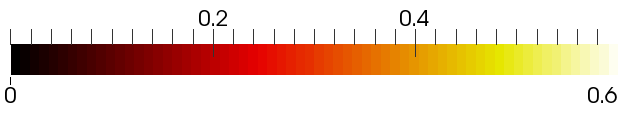
\includegraphics[height = 1cm]{plots/thermalization_urqmd/E80b6_x_paraview_color_legend_for_cuts.png} \\
  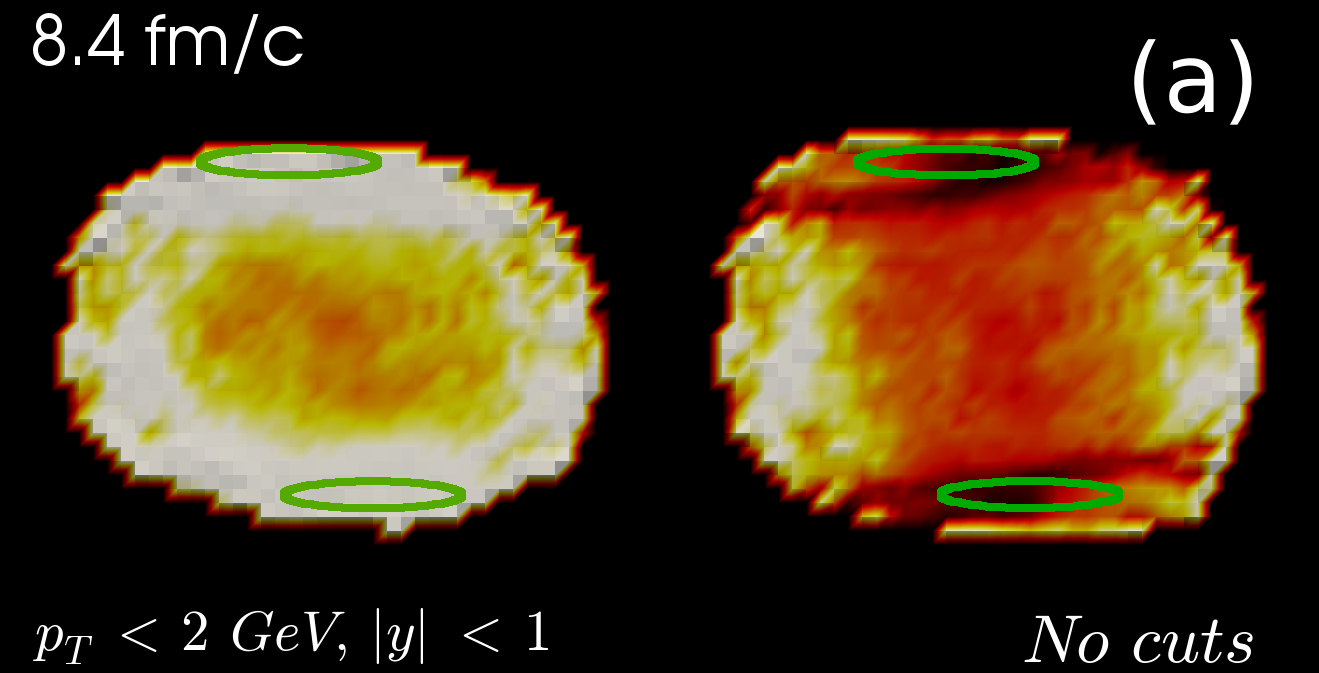
\includegraphics[width = 10cm]{plots/thermalization_urqmd/E80b6_x_paraview_cuts_comparison_t_8_4fm.png}
  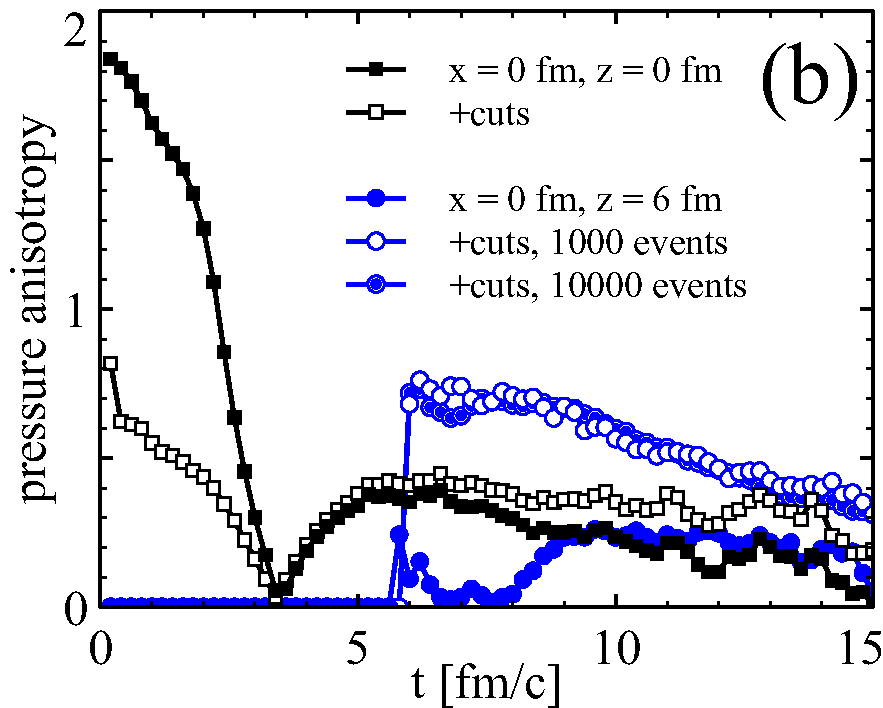
\includegraphics[width = 10cm]{plots/thermalization_urqmd/E80b6_x_vs_t_few_space_points_with_cuts.pdf}
   \caption{The effect of $p_T < 2$ GeV and $|y| < 1$ cuts on the space
            distribution of the pressure anisotropy $X =
            \frac{|T_L^{11}-T_L^{22}|+|T_L^{22}-T_L^{33}|+|T_L^{33}-T_L^{11}|}
            {T_L^{11}+T_L^{22}+T_L^{33}}$
            (see color scale above the Fig.) for collision energy 
            $\Elab = 80$ \emph{A} GeV and impact parameter $b = 6$ fm.
            If the value of $X$ exceeds color map maximum, it is marked with the same
            color as maximum. Solid lines mark the positions of the nuclei, if they
            would not interact.}
\label{FIG:X_paraview_cuts_effect}
\end{figure}

Previously, all participants were included into the $\Tmn$ calculation. However, it
is generally believed that soft particles at midrapidity thermalize faster,
therefore it might be insightful to impose cuts in momentum space, if one wants
to obtain a more isotropic $\Tmn$. On the other hand, applying transverse
momentum $p_T$ and rapidity $y$ cuts on a perfectly symmetric distribution
results in an asymmetry. In addition, these cuts decrease the statistics, which
leads to an increase of the anisotropy. To study the effect of the kinematic
cuts on the space distribution of the pressure anisotropy $X$, $\Tmn$ was
constructed only from particles with $p_T < 2$ GeV and $|y| < 1$ . The effect of cuts
on $X$ over space is shown in Fig. \ref{FIG:X_paraview_cuts_effect}. The statistical
effect does not play a significant role, because the results do not change after
increasing the number of events from $N_{ev} = 10^3$ to $10^4$. The large anisotropy
at very early times decreases after imposing cuts. But the anisotropy at later times
is strikingly larger with cuts, first of all in the regions behind the nuclei. While
without cuts it was possible to introduce an ''isotropization time'', when $X$ is
smaller than $0.3$ at more than 50\% of the area, with the cuts the anisotropy is so
high all over the space that the isotropization time cannot be introduced anymore.

\section{Summary and discussion}

The assumption of rapid equilibration was tested at $\Elab = $ = 5--160
\emph{A} GeV using the coarse-grained UrQMD transport approach.  The
energy-momentum tensor was studied locally in space and time and its deviation
from the ideal fluid form was quantified with two numbers: the pressure
anisotropy $X$ and the off-diagonality $Y$. First of all, it was shown that $X$
and $Y$ depend on the number of UrQMD events $N_{ev}$ used to construct $\Tmn$.
Low statistics implies large deviations, even if the underlying distribution
function is completely thermal and isotropic. An initial state constructed from
less than a few hundred events (or a few hundred testparticles equivalently) is
bound to deviate strongly from the ideal fluid form. The off-diagonality
appears to be mostly produced by this statistics effect. For large statistics
$Y$ tends to be small in all the collision region at all times. The pressure
anisotropy does not vanish with large statistics, it is a physical effect related
to the anisotropy of the underlying distribution function
$\mathit{f}(\vec{r},\vec{p})$. As a consequence, the initial state from UrQMD
with enough statistics is suitable for anisotropic hydrodynamics.

Unfortunately, all the results depend on the smearing parameter $\sigma$. With
larger $\sigma$ isotropization is reached later, but the degree of
isotropization is higher. From a practical point of view that means that
selecting large $\sigma$ one has to take larger fluidization time. This is in
agreement with conclusion of \cite{Petersen:2010zt} that a larger fluidization
time should be taken for larger $\sigma$ to obtain the same pion yield.
However, strictly speaking, the physical limit is $\sigma \to 0, \, \sigma^3
\rho N_{ev} \to \infty$. It was found that at small $\sigma$ the isotropization
time approaches the time of geometrical criterion $t_{geom} = 2R
(\Elab/2m_N)^{-1/2}$, so the rapid isotropization at the time of geometrical
overlap is partly justified, but only in the above mentioned limit. In the
existing models the smearing parameters and statistics are such that at
$t_{geom}$ the anisotropies are very high.

For the pressure anisotropy $X$ it was observed, that it exhibits a similar
pattern for all the considered collision energies and centralities: there is a
narrow interval of time, when it rapidly drops in a considerable volume. This
feature allowed us to introduce and study the isotropization time $t_{iso}$.
The time $t_{iso}$ can be considered as the time, when UrQMD starts to be
compatible with viscous hydrodynamics. At $t < t_{iso}$ the pressure anisotropy
$X$ is too high for viscous hydrodynamics to be applied. Isotropization time
decreases with collision energy, following the same trend as the geometrical
overlap time.  Based on this finding a new fluidization criterion is suggested:
$t_{iso} = t_{geom}(E) + \Delta t_0 (\sigma)$, where $\Delta t_0$ depends only
on the Gaussian smearing $\sigma$ and can be determined from
Fig.~\ref{FIG:t_iso_sensitivity_sigma}. A slight dependence of the isotropization
time on centrality was observed: it increases with impact parameter, but the
slope of this increase becomes smaller and smaller for higher energies. This
behaviour has a simple geometrical interpretation.

  \chapter{Cooper-Frye contributions in Au+Au collisions at $\Elab = 5$--$160$ \emph{A} GeV}
\label{chap:cooper_frye}

%\chapterquote{}{}

In most heavy ion collision simulations involving relativistic hydrodynamics,
the Cooper-Frye formula (see section \ref{sec:cf_explanation}) is applied to
transform the hydrodynamical fields to particles. As it was discussed in
section \ref{sec:cf_explanation}, under certain circumstances Cooper-Frye
formula can produce negative numbers of particles, the so-called negative
contributions. Here the magnitude of negative contributions is investigated as
a function of the hadron mass, collision energy in the range of $\Elab = 5$--$160$
\emph{A} GeV, collision centrality and the energy density transition criterion defining
the particlization hypersurface. The microscopic results are compared to
negative contributions expected from hydrodynamical treatment assuming local
thermal equilibrium. This chapter is based on publication \cite{Oliinychenko:2014tqa}.


\section{Methodology}
\label{sec:cf_Methodology}

The calculation is based on the hadronic transport approach - Ultra-relativistic
Quantum Molecular Dynamics (UrQMD 3.3p2) \cite{Bass:1998ca,Bleicher:1999xi},
already introduced in chapter \ref{chap:local_equilibration}.  In this study no
long-range potentials  are included and particle trajectories between
collisions are always straight lines. Au + Au collisions are simulated with
UrQMD at laboratory frame energies $\Elab =$ 5, 10, 20, 40, 80 and 160 \emph{A} GeV.
This energy region is chosen because UrQMD provides a reasonable description of
the collision dynamics at those energies, and the Cooper-Frye negative
contributions are expected to become significant in this energy range.

The general procedure for our calculations is:

\begin{enumerate}

\item Generate many UrQMD events and coarse-grain them on a 3+1D Cartesian
  space-time grid. The energy-momentum tensor $\Tmn$ and baryon four-current $\jmu_B$
  are computed as described in the section \ref{sec:coarse_graining}.  The grid
  cell sizes need to be small enough, so that gradients of all relevant physical
  quantities within the cell are small. On the other hand, if the cell sizes are
  too small one needs to generate infeasibly many events to damp statistical
  fluctuations of the $T^{\mu \nu}$ components from cell to cell, and obtain a smooth
  surface $\Sigma$. To satisfy these conditions and to ensure energy conservation
  precisely we choose $\Delta x = \Delta y = $ 1 fm, $\Delta z$ = 0.3 fm and time
  step $\Delta t$ = 0.1 fm. For the highest collision energy, $\Elab =
  160A$ GeV, the gradients are larger, so even smaller grid sizes were taken:
  $\Delta x = \Delta y = $ 0.3 fm and $\Delta z$ = 0.1 fm. This choice is further
  discussed in the section \ref{sec:cf_Tests}, where the sensitivity of results
  to the grid size is studied. As discussed further in the section \ref{sec:cf_Tests}
  $N$ = 1500 events are enough to obtain stable results.

\item Find the local energy density in the Landau rest frame of each grid cell,
  $\epsilon_{LRF}(t,x,y,z)$, and the collective flow velocity in each cell,
  $\vec{v}(t,x,y,z)$ as described in section \ref{sec:fluidization}, according to
  Eq. (\ref{eq:lrf}).  To apply the Cooper-Frye formula one needs the temperature
  $T$ and chemical potentials, which do not exist in the microscopic picture.
  Strictly speaking they make sense only in the vicinity of thermal and chemical
  equilibrium, which may not be the case in our UrQMD simulation. Nevertheless,
  the Landau rest frame energy density and net baryon density obtained from UrQMD
  are substituted to the ideal hadron resonance gas equation of state (Eqs.
  \ref{eq:id_hadgas_eos1}-\ref{eq:id_hadgas_eos3}) to obtain $T$ and chemical
  potentials, as in the case when deviations from equilibrium are small.  The
  particle list in the equation of state coincides with the list of particles in
  UrQMD. Zero strangeness density is assumed, even if UrQMD itself allows local
  non-zero strangeness.

\item Construct the hypersurface $\Sigma$ of a constant energy density
  $\epsilon_{LRF}(t,x,y,z) = \epsilon_c$.  In this way the transition surface
  in hybrid models is mimicked, which is typically constructed at energy densities
  $\epsilon_c = 0.3$--1 GeV/fm$^3$~\cite{Huovinen:2012is}.  The isosurface is
  constructed using the Cornelius subroutine~\cite{Huovinen:2012is}, that provides a
  continuous surface without holes and avoids double counting of hypersurface pieces.
  The subroutine provides the normal four-vectors $d\sigma_{\mu}$ of the hypersurface.
  The physical quantities on the grid, \emph{i.e.}, the energy, net baryon density
  and the flow velocity, are linearly interpolated to the geometrical centers of
  the hypersurface elements.

\item Calculate the particle spectra on $\Sigma$ by using the
  Cooper-Frye formula and by counting the actual UrQMD particles that
  cross $\Sigma$.  To obtain these spectra and to compare them to each
  other is the goal of the computation.

\end{enumerate}

This procedure mimics switching from hydrodynamics to transport in a
hybrid model, but here the ''hydrodynamical'' picture is obtained by
averaging over particle distributions on a space-time grid. Since all
the information is still available in the underlying microscopic
approach, it was possible to compare the negative Cooper-Frye contributions
to the spectrum of actual backscattered particles.

Cooper-Frye formula is applied on the hypersurface. The spectrum from
the Cooper-Frye formula is split into positive and negative parts:

\begin{eqnarray}
\label{Eq:CFdef1}
\frac{dN^{+}_{CF}}{p_T dp_T d\varphi dy }
  & = & \frac{g}{(2\pi)^3}
         \int_{\sigma}\frac{\Theta(p^{\mu}d\sigma_{\mu}) \, p^{\mu}d\sigma_{\mu}}
         {e^{(p^{\nu}u_{\nu}-\mu)/T} \pm 1} \\
\label{Eq:CFdef2}
\frac{dN^{-}_{CF}}{p_T dp_T d\varphi dy }
  & = & \frac{-g}{(2\pi)^3}
         \int_{\sigma}\frac{\Theta(-p^{\mu}d\sigma_{\mu}) \,p^{\mu}d\sigma_{\mu} }
         {e^{(p^{\nu}u_{\nu}-\mu)/T} \pm 1}
\end{eqnarray}

To evaluate $dN/dy$ or $dN/p_T dp_T$ the integrations are performed
numerically, applying the 36$\times$36 points Gauss-Legendre method to
integrals transformed to finite limits.

For comparison with the Cooper-Frye calculation we count the actual microscopic
particles crossing the same hypersurface $\Sigma$ that is used for Cooper-Frye
calculations. Inward and outward crossings are counted separately. Note that
$\epsilon > \epsilon_c$ inside the surface and $\epsilon < \epsilon_c$ outside
of it. This is used to find where a particle trajectory crosses $\Sigma$: the
energy density is interpolated to the particle trajectory to find the point
where $\epsilon - \epsilon_c$ changes sign.  Each crossing of $\Sigma$ is
counted as positive, if the particle streams outward and negative, if the
particle flies toward higher energy densities.

Both the Cooper-Frye calculation and the particle counting start at the same time
$t_{start}$, which depends on the collision energy. Following the prescription
from hybrid models, $t_{start} = \frac{2R}{v\gamma}$ is taken.  This is the
time two nuclei need to pass through each other. Numerical values are shown in
Tab. \ref{tab:tstart}. The same $t_{start}$ is used for all centralities.

\begin{table}
  \begin{tabular}{rc}
  \toprule
  $\Elab$, \emph{A} GeV    &  $t_{start}$, fm/c \\
  \midrule
      5                    &       8.0        \\
      10                   &       5.6        \\
      20                   &       4.0        \\
      40                   &       2.8        \\
      80                   &       2.0        \\
     160                   &       1.4        \\
  \bottomrule
  \end{tabular}
  \caption{The geometrical overlap time $t_{start}$ versus collision energy $\Elab$.
           Both the Cooper-Frye calculation and the particle counting start at the
           time $t_{start} = \frac{2R}{v\gamma}$.}
  \label{tab:tstart}
\end{table}

\section{Sensitivity to internal parameters and fulfillment of
  conservation laws}
\label{sec:cf_Tests}

\begin{figure}[htp]
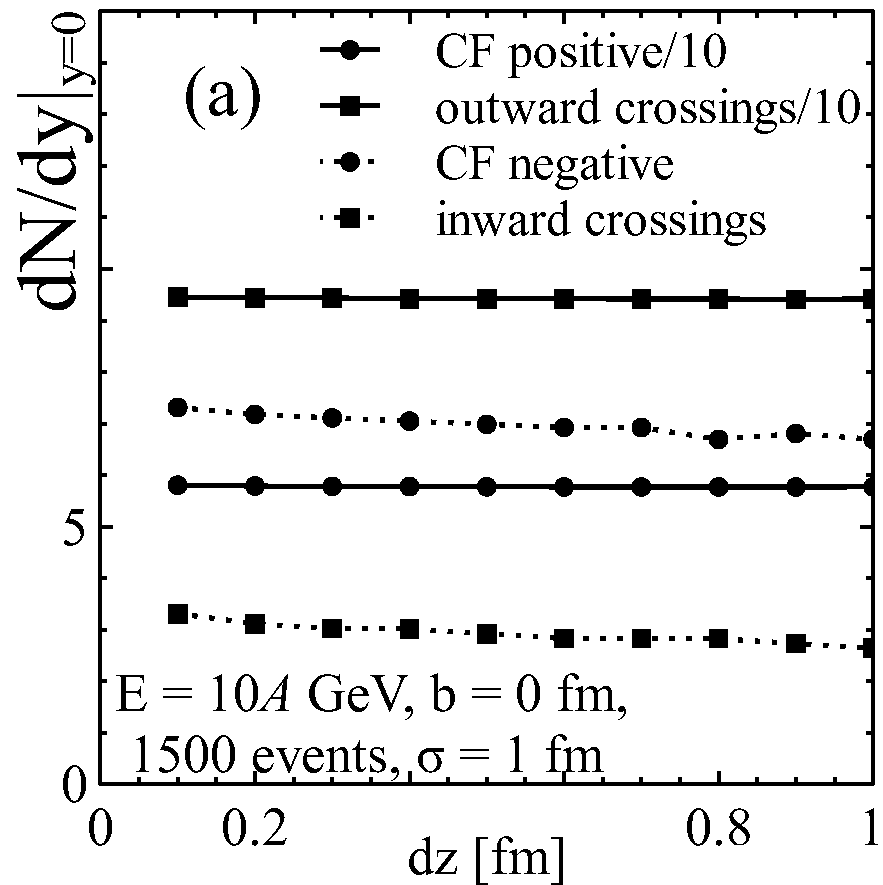
\includegraphics[height=4.6cm]{plots/cooper_frye/dz.pdf}
\includegraphics[height=4.6cm]{plots/cooper_frye/ev.pdf}
\includegraphics[height=4.6cm]{plots/cooper_frye/sig.pdf}
\caption{Sensitivity of results to internal parameters of the
  simulation: grid spacing along z axis, $dz$ (a), number of
  events, N (b) and the width $\sigma$ of Gaussian
  smearing (c). }
\label{Fig:Int_par}
\end{figure}

\begin{figure*}[htp]
\includegraphics[height=7cm]{plots/cooper_frye/Econs.pdf}
\caption{ Energy flux through the surface at different
  times evaluated as actual flow,
  $\Delta E_1(t)/dt = \int_{t-dt}^{t} T^{\mu 0} d\sigma_{\mu}/dt$
  (circles), and as a difference in energy within the surface at
  different times, $\Delta E_2(t)/dt = (E_{in}(t) - E_{in}(t-dt))/dt$
  (rectangles). Lower panel shows the relative difference between
  these two measures in \%, and thus the conservation of energy in the
  calculation.}
\label{Fig:Econs}
\end{figure*}

Besides physical parameters like the beam energy, $\Elab$, and
centrality of the collision controlled by the impact parameter $b$,
our simulation contains internal parameters like grid spacing, the
width of the smearing Gaussian $\sigma$, and the number of events $N$.
Ideally, one should work in a region of internal parameters, where the
results are independent of them. To see how sensitive our results
are to these internal parameters, the positive and negative
contributions to the pion yield at midrapidity,
$\frac{dN}{dy}|_{y=0}$, at different values of these parameters are
evaluated.

The calculation is more sensitive to the grid spacing in z direction,
$dz$, than to the spacings in x and y directions, $dx$ and $dy$, since
gradients of $T^{\mu\nu}$ are largest in the longitudinal
direction. Although, as shown in Fig.~\ref{Fig:Int_par}~a), even the
sensitivity to $dz$ is weak over a reasonable range of values. The
main motivation for choosing the grid spacing and time step comes in
fact from the requirement of energy conservation discussed later.

The results are very sensitive to the small number of events (see
Fig.~\ref{Fig:Int_par}~b), but already $N = 500$ events provides
sufficient statistics for stable results.  To be on the safe side, we
have analyzed $N=1500$ events for our final results. Unfortunately,
our results are not completely independent of the width $\sigma$ of
the Gaussian smearing, as shown in Fig.~\ref{Fig:Int_par}~c). The
number of inward crossing UrQMD pions is most sensitive to
$\sigma$. Two effects play a role here: for small $\sigma$ the surface
still has large statistical fluctuations and small scale structures,
``lumps'' (See Fig.~2 of Ref~\cite{Huovinen:2002im}), whereas at large
$\sigma$ the smearing pushes transition surface further out in
space. Further out the densities are smaller, and the UrQMD particle
distributions are further away from equilibrium so that especially the
number of particles moving toward the center is strongly reduced.  We
choose $\sigma = 1$ fm as a reasonable value for our calculations, but
keep in mind that varying $\sigma$ in the range from 0.6 fm to 1.4 fm
causes $\sim$ 20 \% difference in the number of inward crossings. We
consider this a systematic error in our analysis, but fortunately this
uncertainty does not affect our main conclusions.

To check that energy is conserved in the coarse-graining procedure, we
evaluate the energy flow through the surface during the time step
$dt$, $\Delta E_1(t) = \int_{t-dt}^{t} T^{\mu 0} d\sigma_{\mu}$, and
compare it to the change in energy within the surface during the same
time step, $\Delta E_2(t) = E_{in}(t) - E_{in}(t-dt)$, where $E_{in}$
is total energy of particles inside the surface. Ideally
$\Delta E_1(t) = \Delta E_2(t)$ for any $dt$, but finite cell sizes
limit the precision and break the conservation of energy. The accuracy
of $\Delta E_1 \approx \Delta E_2$ improves when grid spacing and time
step are decreased. Fig.~\ref{Fig:Econs} shows the energy flux
through the surface and the relative difference between
$\Delta E_1(t)$ and $\Delta E_2(t)$ in central collisions at energies
$\Elab = 10$, 40, 160$A$ GeV. To achieve better than 5\% percent
accuracy at all times, small grid spacing is used with
$\Delta x = \Delta y = 1$ fm, $\Delta z$ = 0.3 fm, and time step
$\Delta t$ = 0.1 fm/c in collisions with $\Elab \le 80A$ GeV,
and an even finer grid with $\Delta x = \Delta y = 0.3$ fm, and
$\Delta z = 0.1$ fm for collisions at $\Elab = 160A$ GeV. When
integrated over the whole collision time, the violation of energy
conservation is less than 1\% at all collision energies. A similar check was performed
for the net baryon charge, and similar results were obtained.


\section{Magnitude of negative Cooper-Frye contributions estimated from the coarse-grained transport approach}
\label{sec:cf_Results}

\begin{figure}[htp]
\includegraphics[height=6cm]{plots/cooper_frye/TZ.pdf}
\includegraphics[height=6cm]{plots/cooper_frye/T_on_surf.pdf}
\caption{ Upper panel: Hypersurface of constant LRF
  energy density $\epsilon(t,0,0,z) = \epsilon_c = 0.3$
  GeV/fm$^3$. Lower panel: The fraction of hypersurface elements with
  (apparent) temperature $T$ in central Au+Au collisions at the
  collision energy of $\Elab = 5$, 10, 20, 40, 80, 160$A$ GeV.}
\label{Fig:surf}
\end{figure}

Let us start by investigating the properties of the transition
hypersurface itself as a function of beam energy. Figure
\ref{Fig:surf} depicts the surface $\Sigma$ in longitudinal direction
along the x axis. One can see that with increasing energy, the lifetime of
the system increases. This indicates longer lasting surface emission
(from space-like parts of the surface), which might lead to larger
negative contributions. On the other hand, with increasing energy the
longitudinal expansion leads to a larger volume of the final volume
emission (from time-like parts of the surface), which indicates
smaller negative contributions. Thus there are two competing effects,
and one has to carry out the actual calculation to find out how the
negative contributions depend on energy.

Distributions of the (apparent) temperature of the hypersurface
elements are shown on the right panel of Fig.~\ref{Fig:surf}. At each
collision energy the temperature distribution is rather narrow, which
means that the constant energy density surface approximately coincides
with a constant temperature surface. As well, the average temperature
increases with increasing collision energy as expected from thermal
model fits to particle yields~\cite{Andronic:2008gu}.

\begin{figure}[htp]
\includegraphics[width=5cm]{plots/cooper_frye/E40pi.pdf}
\includegraphics[width=5cm]{plots/cooper_frye/E40Kmi.pdf}
\includegraphics[width=5cm]{plots/cooper_frye/E40N.pdf}
\caption{ Rapidity distribution of identified particles
  obtained from Cooper-Frye formula on the surface $\Sigma$ and from
  explicit counting of particles that cross the same surface. Positive
  contributions and the net distribution, \emph{i.e.},
  positive-negative, are shown separately. 
  Central Au+Au collisions at $\Elab = 40$ \emph{A} GeV}
\label{Fig:spectra}
\end{figure}

Fig.~\ref{Fig:spectra} compares rapidity spectra of identified
particles in Au+Au collisions at $\Elab = 40$ \emph{A} GeV obtained by
Cooper-Frye calculation and by counting of the microscopic
particles. Even though, the results only for one
collision energy are shown, all results are qualitatively the same at all other
energies. If UrQMD is close to equilibrium on a surface at
$\epsilon_c = 0.3$ GeV/fm$^3$, both approaches should yield similar
distributions. At midrapidity this is the case for nucleons, and with
a lesser accuracy for kaons. $\Delta$'s, $\Lambda$'s, $\rho$'s and
$\eta$'s which are not shown in the figure depict a behavior similar
to nucleons. However, the pion yields are wildly different indicating
that pions are---and thus the entire system is---far away from
chemical equilibrium at least. To cancel the effect of
non-equilibrium and to visualize the differences in momentum distributions
we consider not the absolute value of the negative
contributions, but the ratio of negative to positive ones,
$(dN^-/dy)/(dN^+/dy)$ or $(dN^-/dp_T)/(dN^+/dp_T)$. From
Fig. \ref{Fig:spectra} it is also apparent that the magnitude of the
negative contributions is always small compared to the positive ones
as expected.


\begin{figure}[htp]
\includegraphics[width=7cm]{plots/cooper_frye/neg_contr_mass.pdf}
\caption{ Rapidity distribution of the ratio of negative
  to positive contributions for different hadron species: pions
  (circles), $K^{+}$ (crosses), $\rho$ (bars), nucleons (rectangles),
  and deltas (triangles).  Cooper-Frye calculation in central Au+Au
  collisions at $\Elab = 40A$ GeV.}
\label{Fig:neg_contr_pmass}
\end{figure}

The dependence of the ratio $(dN^-/dy)/(dN^+/dy)$ on the hadron type
is illustrated in Fig.~\ref{Fig:neg_contr_pmass} by the Cooper-Frye
results. Since for all cases, the microscopic negative contributions
of backstreaming particles are much smaller than the Cooper-Frye ones
we concentrate on showing the maximal effect. Surface temperature and
velocity profiles are identical for all hadrons, so the plot
demonstrates first of all the effect of particle mass. One can see
that the average value of $(dN^-/dy)/(dN^+/dy)$ decreases with
particle mass. This can be understood by considering a small volume of
fluid in its rest frame, and a space-like surface moving through it
with a velocity $0<v_{surf}<c$ so that lower density, \emph{i.e.},
outside, is in the negative direction. To be counted as a negative
contribution, a particle must enter the fluid, and thus have a larger
velocity than the surface. Average thermal velocity decreases with
increasing mass, and therefore the heavier the particle, the fewer of
them cross the surface inward. Since relative negative contributions
for pions are several times larger than for other hadrons,
in the following only pions will be considered.


\begin{figure}[htp]
\includegraphics[width=7cm]{plots/cooper_frye/neg_vs_E.pdf}
\caption{ The ratio of negative to positive
  contributions on the $\epsilon(t,x,y,z) = \epsilon_c = 0.3$
  GeV/fm$^3$ surface for pions at midrapidity in central Au+Au
  collisions at various collision energies. Circles depict Cooper-Frye
  result and rectangles the explicit counting of UrQMD particles.}
\label{Fig:neg_contr_Ecoll}
\end{figure}

As could be seen in Fig.~\ref{Fig:spectra}, imposing equilibrium for
Cooper-Frye calculation leads to significantly larger negative to
positive contribution ratio at midrapidity than the counting of UrQMD
particles. As shown in Fig.~\ref{Fig:neg_contr_Ecoll} this holds for
all the considered energies, showing that the system is out of
not only chemical, but also of kinetic equilibrium. Either the
collective flow velocity of pions is different from the collective
velocity of other particles \cite{Sorge:1995pw,Pratt:1998gt} or the
dissipative corrections to pion distribution are very large. It was
also checked that the relative microscopic negative contributions are
much smaller in UrQMD at all centralities, for all particle species,
and on isosurfaces of energy density $\epsilon_c = 0.3$ and 0.6
GeV/fm$^3$.

On the other hand, the trend as a function of collision energy in
Cooper-Frye and UrQMD calculations is the same: both curves have a
maximum at 10-20$A$ GeV and then decrease with increasing energy. This
behavior is a result of a complicated interplay of several factors:
temperature, relative velocities between surface and fluid, and
relative amounts of volume and surface emission, \emph{i.e.}, emission
from the time- and space-like parts of the surface. To gain some
insight all these factors are considered separately. The same argument
used to explain the sensitivity of negative contributions to particle
mass, explains why larger temperature leads to larger negative
contributions. Temperature on the constant density surface grows with
increasing collision energy (see Fig.~\ref{Fig:surf}), which would
lead one to expect an increase of negative contributions with
increasing collision energy. On the other hand, larger relative
velocity between the fluid and surface reduces the negative
contributions (again the same argument), and one can see that the average
relative velocity increases with increasing collision energy. Finally,
as argued when discussing Fig.~\ref{Fig:surf}, the
larger the collision energy, the larger the fraction of volume
emission. Which, as mentioned, reduces the negative contributions.

\begin{figure}[htp]
\includegraphics[width=7cm]{plots/cooper_frye/pt_binned_negcontr_pi_E40rebinned.pdf}
\caption{ The ratio of negative to positive pion
  contributions as a function of transverse momentum at midrapidity in
  central Au+Au collisions at $\Elab = 5$, 10, 20, 40, 80$A$ GeV.}
\label{Fig:neg_contr_pt}
\end{figure}

It is instructive to evaluate the negative contributions as function
of transverse momentum $p_T$ as well, as shown in
Fig.~\ref{Fig:neg_contr_pt} for Cooper-Frye calculation and "by
particles". One can see that the largest negative contributions are
located at small $p_T$, which means that one can reduce the
uncertainty caused by the negative contributions by a low $p_T$
cut. Also as a function of transverse momentum, the amount of
microscopically backward streaming particles is much smaller than in
an equilibrium scenario.

When discussing Fig.~\ref{Fig:neg_contr_Ecoll} it was mentioned that,
independent of the energy density of the surface, the negative
contributions are much smaller when counting the UrQMD
particles. Furthermore, in Cooper-Frye calculations the strength of
the negative contributions depends on the value of $\epsilon_c$ where
the distributions are evaluated as shown in
Fig.~\ref{Fig:neg_contr_e0}. Larger $\epsilon_c$ leads to larger
negative contribution at midrapidity and lower at back- and forward
rapidities. This result arises from interplay of two factors: larger
temperature and smaller average $v_{rel}$ for larger energy
density. Quite surprisingly the negative contributions evaluated by
counting the UrQMD particles is almost independent of the value of
$\epsilon_c$. This indicates that even in much higher temperature
$T\sim 155$--160 MeV the microscopic system is not fully thermalised.

\begin{figure}[htp]
\includegraphics[width=7cm]{plots/cooper_frye/piym_new.pdf}
\caption{ Rapidity distribution of the ratio of negative
  to positive contributions for pions on
  $\epsilon(t,x,y,z) = \epsilon_c = 0.3$ GeV/fm$^3$ (circles) and
  $\epsilon_c = 0.6$ GeV/fm$^3$ (crosses) surfaces in central Au+Au
  collisions at $\Elab = 40\ A$ GeV. Full symbols correspond to
  Cooper-Frye calculation and open symbols to explicit counting of
  UrQMD particles.}
\label{Fig:neg_contr_e0}
\end{figure}

The dependence of the contribution ratio on centrality is shown in
Fig.~\ref{Fig:neg_contr_b}. The negative contributions decrease with
decreasing centrality because the more peripheral the collision, the
larger the fraction of time-like hypersurface elements. This behavior
is illustrated in the right panel of Fig.~\ref{Fig:neg_contr_b}. In
the limit of very peripheral collisions the lifetime of the system
becomes zero, and thus the surface is time-like everywhere and there
are no negative contributions at all. Temperature and relative
velocities appear to be less important factors in this case than the
relative amount of time-like and space-like hypersurface elements.

\begin{figure}[htp]
\includegraphics[height=7cm]{plots/cooper_frye/neg_contr_b_v2.pdf}
\includegraphics[height=7cm]{plots/cooper_frye/TZ_vs_b.pdf}
\caption{ Upper panel: Rapidity distribution of the
  ratio of negative to positive contributions for pions in Au+Au
  collisions at $\Elab = 40\ A$ GeV at various centralities: $b=0$
  (circles), $b = 6$ fm (crosses) and $b = 12$ fm (rectangles). Lower
  panel: hypersurfaces along the z axis in the same collisions at the
  same centralities.}
\label{Fig:neg_contr_b}
\end{figure}

Let us finally compare our results to previous studies. In
\cite{Huovinen:2012is} negative contributions were evaluated on the
$\epsilon = 0.3$ GeV/fm$^3$ transition surface of a hybrid model at
SPS and RHIC energies---$\Elab = 160A$ GeV and
$\sqrt{s_\mathrm{NN}} = 200$ GeV, respectively---and found to be
around $(dN^{-}_{\pi}/dy)/(dN^{+}_{\pi}/dy) \simeq$ 13\% and 9\% at
$y=0$. The negative contributions for 160$A$ GeV are slightly larger
than in our calculation. The reason for this discrepancy lies in the
difference of the velocity profiles on the hypersurfaces: In
hydrodynamics the average relative velocity between flow and surface
is smaller than in our transport-based approach, which leads to larger
negative contributions.

\section{Summary and discussion}

The assumptions of hybrid and hydrodynamical approaches at the end of the
hydrodynamical evolution lead to the appearance of Cooper-Frye negative
contributions - negative numbers of particles produced by the Cooper-Frye
formula at particlization on the hypersurface elements with a space-like
normal. At high collision energies at midrapidity --- the kinematic region probed by
RHIC and LHC --- the Cooper-Frye negative contributions are negligible. However,
at intermediate energies they were not studied before.

Here negative Cooper-Frye contributions and
backscattering were investigated using a coarse-grained transport
approach. Au+Au collisions at $\Elab = 5$--$160\ A$ GeV energies have
been simulated with UrQMD, and a hypersurface $\Sigma$ of constant
Landau rest frame energy density has been constructed. On this surface
two quantities were computed: The ratio of Cooper-Frye negative
to positive contributions, which assumes local thermal equilibrium,
and the ratio of UrQMD particles crossing $\Sigma$ inward to crossing
$\Sigma$ outward, which assumes no equilibrium.

It was found that at all collision energies the ratio of inward to outward
moving particles calculated counting the UrQMD particles is much
smaller than the same ratio calculated assuming equilibrium,
\emph{i.e.}, the Cooper-Frye negative to positive ratio. This finding
poses a question to the construction of hybrid models, and the
treatment of freeze-out in hydrodynamical models: If the cascade leads
to distributions nowhere near equilibrium, how are the hydrodynamical
and cascade stages to be connected in a consistent fashion? On the
other hand, this result shows that an ideal fluid dynamics hybrid
approach contains the worst case scenario for negative contributions
and even then they are on the order of max.~$15\%$ for the pion yield
at midrapidity. What remains to be seen, however, is whether one could
get closer to the UrQMD result with dissipative corrections
to the distribution function of Cooper-Frye, or whether the deviations
from equilibrium are so large that dissipative expansion is not
feasible.

The largest observed impact of negative contributions is to pion
rapidity spectrum at midrapidity in central collisions. In thermally
equilibrated Cooper-Frye calculations it constitutes 8--13\%, but only
0.5--4\% in the counting of UrQMD particles. The Cooper-Frye value
roughly agrees with the values obtained previously for hydrodynamics
at 160 GeV. Several systematic features were found in these ratios. They
are smaller for larger hadron mass and therefore largest for
pions. The relative negative contributions decrease as a function of
collision energy and by going from central to peripheral
collisions. On the other hand, they increase if a higher energy
density is chosen as a surface criterion. The small scale structures
on the surface, its ``lumpiness'', play a significant role: If the
surface is not smooth enough both ratios can increase
dramatically. Therefore, an interesting future study could be to
compare single fluctuating events to the averaged result.

  \chapter{SMASH transport approach: implementation and testing}
\label{chap:smash}

This chapter is largely based on \cite{Weil:2016zrk}.
A significant part of the work on this thesis was devoted to developing
a new transport approach, SMASH (Simulating Many Accelerated
Strongly-interacting Hadrons), which is described in this chapter.
SMASH is used for an investigation carried out in chapter \ref{chap:forced_therm}.
Conceptually the approach is similar to UrQMD, which was used in chapters
\ref{chap:local_equilibration} and \ref{chap:cooper_frye}. The main
difference is that SMASH is a transport
approach of a BUU type, while UrQMD is of QMD type (see section \ref{sec:transport}
for BUU vs. QMD discussion). This difference mainly matters for the
treatment of potentials and in the studies of this thesis potentials are not
included. The reasons to use SMASH in the following investigation are rather
technical than physical: SMASH is developed from scratch under version control,
it is written in C++, it undergoes continuous testing (both from programming and
physics side) and the implementation of forced thermalization approach appeared to be
technically easier in SMASH. The current version of SMASH is 1.0rc, however the
studies in chapter \ref{chap:forced_therm} were performed with an earlier version
SMASH-0.9rc.

As a transport approach SMASH solves a coupled set of Boltzmann
equations (\ref{eq:boltzmann},\ref{eq:buu_icoll}) via the Monte-Carlo method with
the test-particle ansatz

\begin{equation}
  \mathit{f}(x,p) = \frac{1}{N_{test}} \sum \delta^{(3)}(x - x_i) \delta^{(3)}(p - p_i) \,.
\end{equation}

Here every physical particle is represented by $N_{test}$ testparticles,
which sample the distribution function. To simulate the left part of the BUU
equation (\ref{eq:boltzmann}) it is enough to propagate particles according to their
equations of motion. The collision integral (\ref{eq:buu_icoll}) is solved via
simulating particle collisions and decays.

The testparticle ansatz also requires that interaction cross-sections are
modified:

\begin{align}
  \label{eq:testparticles_method1}
  \sigma & \mapsto \sigma \cdot \Ntest^{-1} \\
  \label{eq:testparticles_method2}
  N & \mapsto N \cdot \Ntest
\end{align}

In this way the average scattering rate (number of collisions per unit time per
particle) remains unchanged. The testparticle ansatz has three effects.
Firstly, the more testparticles are used the more precisely the distribution function
$\mathit{f}(x,p)$ is sampled. Due to the geometrical treatment of cross-sections,
particles in SMASH can interact at non-zero distance in contrast to field
theory, where all the interactions are local. So, secondly, the larger $\Ntest$
the smaller are the non-locality effects introduced by the collision criterion.
Thirdly, as shown in \cite{Cheng:2001dz}, experimental observables such as particle
spectra and flow obtained using transport models depend on $\Ntest$ and saturate
when $\Ntest$ is sufficiently large (in case of \cite{Cheng:2001dz}
$\Ntest = 16$ was large enough for saturation).

\section{Degrees of freedom}

The degrees of freedom entering BUU equations in SMASH are hadrons and
strings. The number of coupled BUU equations coincides with the number of degrees
of freedom.

\subsection{Hadrons in SMASH}

All hadrons consisting of the light quarks listed in the Review
of Particle Properties \cite{Agashe:2014kda}, which have an experimental status
''***'' or ''****'', are taken into account in SMASH. This notation for status means
that the existence of these hadrons is experimentally confirmed with high reliability.

The classification of light quark hadrons by quark content using the
$\SUgroup{3}$ flavour group is shown in appendix \ref{sec:SU3}.
These hadrons and their total angular momentum and radial excitations
constitute the hadron spectrum in SMASH.

Currently SMASH has 46 unflavoured mesons, 12 mesons with open strangeness,
17 $N$ baryons, 8 $\Delta$ baryons, 14 $\Lambda$ baryons, 10 $\Sigma$ baryons,
6 $\Xi$ baryons and 2 $\Omega$ baryons. In this counting scheme the whole isospin group
is considered as one particle, for example proton and neutron are counted as one
baryon or the group $\Delta^{++}$, $\Delta^{+}$, $\Delta^{0}$ and $\Delta^{-}$ is
also counted as one $\Delta$ baryon. Antiparticles are also included.

All of these particles are unstable except the proton, but every combination of
 (anti-~)~quarks in a strong-interaction ground state lives long enough, so that in
our simulations it may be considered as stable. A particle is treated as
stable, if its width does not exceed 10 keV (such as the lightest $\pi$, $\eta$, $K$,
N, $\Lambda$, $\Sigma$, $\Xi$, $\Omega$).

Every particle is characterized by the following parameters taken from
experimental data \cite{Agashe:2014kda}: the pole mass, the width at the pole mass,
quantum numbers, decay channels and branching ratios. Branching ratios are assumed to
be independent of mass.

\subsection{Hadron spectral function} \label{sec:spectral_function}

Every unstable hadron is characterized by a spectral function $\mathcal{A}(m^2)$ -
the probability to find it in a state with mass $m$, given that it has
pole mass $M_0$. In SMASH this is implemented by sampling the mass $m$
from the spectral function, when the resonance is produced. The particular
form of $\mathcal{A}(m^2)$ used in SMASH, called relativistic Breit-Wigner function,
can be understood from the following considerations.

The quantum field theory propagator of the particle, including interactions can be
written according to Dyson-Schwinger equation as

\begin{equation}
  \mathcal{G}(p) = \frac{1}{\mathcal{G}_0^{-1}(p) + \Sigma(p)} \,,
\end{equation}

where $G_0(p)$ is the propagator of non-interacting particle and $\Sigma(p)$ is
the so-called self-energy containing quantum loop corrections to the propagator. For
the scalar field

\begin{equation}
  \mathcal{G}_0(p) = \frac{1}{p^{\mu}p_{\mu} - m_{bare}^2} \,,
\end{equation}

where $m_{bare}$ is the bare mass in Lagrangian. For the Lorentz group representations
different from scalars (spinors, vector particles, etc) the propagator is still
proportional to the propagator of the scalar field. Splitting the self-energy
$\Sigma(p)$ into real and imaginary part, one can rewrite the full propagator as

\begin{align}
  \mathcal{G}(p) = \frac{1}{p^{\mu}p_{\mu} - M_0^2 + i \Im{\Sigma(p)}} \\
  M_0^2 = m_{bare}^2 - \Re{\Sigma(p)}
\end{align}

Here $M_0$ is the physical pole mass with interaction correction. This is the
mass taken from experimental data. Now the time-dependent propagator is
the inverse Fourier transformation

\begin{equation} \label{eq:t_dep_propagator}
  \mathcal{G}(t,\vec{p}) = \int \frac{d p^0}{2\pi} e^{i p^0 t}
    \frac{1}{p^{\mu}p_{\mu} - m_0^2 + i \Im{\Sigma(p)}} \,.
\end{equation}

This expression can be interpreted to use in a transport code. The Monte-Carlo
interpretation of the integral in Eq. (\ref{eq:t_dep_propagator}) is the
following: instead of propagating an off-shell particle one can propagate an
on-shell particle with a mass chosen with probability

\begin{align}
  w(m) \sim |m^2 - m_0^2 + i \Gamma(m)|^{-2} \\
  \Gamma(m) = \Im{\Sigma(m)}
\end{align}

In general $\Sigma(p)$ depends on the medium surrounding the particle, which
leads to the off-shell equations of motion \cite{Cassing:2009vt}. However, in
SMASH these in-medium effects are neglected (the effects of accounting them are
discussed in \cite{Cassing:1999mh} and are usually small for hadronic observables).
Therefore all unstable particles
(``resonances'') are assumed to have the shape of a relativistic Breit-Wigner for the
spectral function, resulting in the probability of a resonance with mass $m$:

\begin{equation}
  \mathcal{A}(m^2) = \frac{\mathcal{N}}{\pi} \frac{m \Gamma(m)}{(m^2 - M_0^2)^2 + m^2 \Gamma(m)^2} \,,
\end{equation}

where $\mathcal{N}$ is a normalization factor chosen in such a way that

\begin{equation}
  \int\displaylimits_0^\infty \mathcal{A}(m^2)dm^2 =
  \int\displaylimits_{m_{\textrm min}}^\infty \mathcal{A}(m^2)dm^2 = 1
\end{equation}

\subsection{Resonance width} \label{sec:width}

The total width $\Gamma$ in the previous expression is not constant, but given by the
mass-dependent function $\Gamma(m)$. Each resonance has a minimum mass
$m_\text{min}$ corresponding to the sum of masses of the lightest decay channels,
below which the width, and thus also the spectral function, vanishes. The total width
is computed as the sum of all partial widths:

\begin{equation}
  \Gamma(m)=\sum_i \Gamma_i(m)
\end{equation}

The computation of the decay widths follows the formalism of Manley et
al.~\cite{Manley:1992yb}, where in general the width of a two-body decay
$R\rightarrow ab$ is written as

\begin{equation} \label{eq:off_shell_width}
  \Gamma_{R\rightarrow ab} = \Gamma^0_{R\rightarrow ab} \frac{\rho_{ab}(m)}{\rho_{ab}(M_0)}.
\end{equation}

Here $m$ is the actual off-shell mass of the resonance R, $M_0$ is its pole
mass, $\Gamma^0_{R\rightarrow ab}=\Gamma_{R\rightarrow ab}(M_0)$ is the partial
width at the pole mass and the function $\rho_{ab}$ is defined as

\begin{align} \label{eq:rho_definition}
  \rho_{ab}(m) = \int & dm^2_a dm^2_b \mathcal{A}_a(m^2_a)\mathcal{A}_b(m^2_b) \nonumber \\
               \times & \frac{p_{cm}}{m} B_L^2(p_{cm}R) \mathcal{F}_{ab}^2(m).
\end{align}

In this formula, $m_a$ and $m_b$ denote the (off-shell) masses of the particles
a and b (which are being integrated over), $\mathcal{A}_a$ and $\mathcal{A}_b$
are their spectral functions and $p_{cm}$ is the absolute value of the
final-state momentum of a and b in the center-of-mass frame, which is given by:

\begin{align} \label{eq:p_cm}
  \vec{p}_{cm}^{\,2}(m,m_a,m_b) = \frac{(m^2-(m_a+m_b)^2)(m^2-(m_a-m_b)^2)}{4m^2}
\end{align}

Finally, L is the orbital angular momentum of a and b in the final state and
$B_L$ are the so-called 'Blatt-Weisskopf functions' \cite{BlaWei}. The
parameter $R$ is usually called the 'interaction radius' and is assumed to have
a universal value of $R=1$ fm for all processes. The form factor
$\mathcal{F}_{ab}$ is only relevant for unstable decay products and will be
discussed further.

The simplest case is that of a resonance R decaying into two stable daughter
particles. Popular examples are $\Delta\rightarrow\pi N$ or
$\rho\rightarrow\pi\pi$. In this case, the daughters have fixed masses (i.e.
their spectral functions are just $\delta$ functions), so that the integrals
collapse:

\begin{equation}
  \rho_{ab}(m) = \frac{p_{cm}}{m} B_L^2(p_{cm} R)
\end{equation}

As an example, the width for the p-wave (L=1) decays of the $\rho$ and $\Delta$
(mentioned above) becomes

\begin{equation}
  \Gamma(m) = \Gamma_0 \frac{M_0}{m} \left|\frac{p_{cm}}{p_{cm,0}}\right|^3
              \frac{p_{cm,0}^{\,2}+\Lambda^2}{p_{cm}^{\,2}+\Lambda^2},
\end{equation}

using $B_1^2(x)=x^2/(1+x^2)$. Here $m$ and $M_0$ are the off-shell and pole
mass, respectively, while $p_{cm}$ and $p_{cm,0}$ denote the
final-state momenta in the center-of-mass frame for mass $m$ and $M_0$,
respectively. $\Lambda=1/R$ can be viewed as a cut-off parameter. For an s-wave
(L=0) decay like $\sigma\rightarrow\pi\pi$, the width simply becomes

\begin{equation}
  \Gamma(m) = \Gamma_0 \frac{M_0}{m} \frac{p_{cm}}{p_{cm,0}} \,,
\end{equation}

since $B_0^2=1$.

\begin{figure}
  \centering
  \includegraphics[width=0.8\textwidth]{plots/smash/width.pdf}
  \caption{Total and partial decay widths of the $N^*(1440)^+$ resonance
           as a function of mass. The vertical and horizontal dashed lines
           mark the pole mass and width.}
  \label{fig:width}
\end{figure}

In the case that one of the daughter particles is itself a resonance, the width
calculation becomes more difficult, since the mass of this daughter resonance
is not fixed and needs to be integrated over. Examples for this case are
$N^*(1440)\rightarrow\pi\Delta$ or $\omega\rightarrow\pi\rho$. As one of the
daughters is stable, at least one of the two integrals collapses:

\begin{equation} \label{eq:decay_semistable}
  \rho_{ab}(m) = \int \displaylimits_{m_a^{\textrm min}}^{m-m_b} dm^2_a
         \mathcal{A}_a(m^2_a) \frac{p_{cm}}{m} B_L^2(p_{cm} R)
         \mathcal{F}_{ab}^2(m)
\end{equation}

The remaining integral runs from the minimum allowed mass of particle a (i.e.
the threshold of its lightest decay channel) up to the maximum possible mass of
a in the decay process (given by $m-m_b$). The form factor $\mathcal{F}_{ab}$
(by M. Post \cite{Post:2003hu}) is used only if unstable decay products are
involved and is defined as

\begin{equation} \label{eq:post_ff}
  \mathcal{F}_{ab}(m) =
   \frac{\lambda^4+1/4(s_0-M_0^2)^2}{\lambda^4+\big(m^2-1/2(s_0+M_0^2)\big)^2},
\end{equation}

where the cut-off factors given in the table \ref{tab:cut-off} are used.

\begin{table}
\caption{Cut-off parameter $\lambda$ for form factor in resonance decay widths.}
\label{tab:cut-off}
\begin{tabular}{lc}
\toprule
 decay & $\lambda$ [GeV] \\
\midrule
 $\pi\rho$                                   & 0.8 \\
 unstable mesons (e.g. $\rho N$, $\sigma N$) & 1.6 \\
 unstable baryons (e.g. $\pi\Delta$)         & 2.0 \\
 two unstable daughters (e.g. $\rho\rho$)    & 0.6 \\
\bottomrule
\end{tabular}
\end{table}


It is easy to see that $\mathcal{F}_{ab}(M_0)=\mathcal{F}_{ab}(\sqrt{s_0})=1$.
Note that this form factor was not used by Manley originally, but was added
only later in the GiBUU implementation. The effect of the form factor is that
it suppresses the high-mass tail ($m>M_0$) and slightly enhances the low-mass
tail ($m<M_0$). Both of these effects get stronger with decreasing $\lambda$
($\mathcal{F}_{ab}\rightarrow 1$ for $\lambda\rightarrow\infty$). In this aspect
SMASH follows the GiBUU framework for the width parametrization of
resonances, since it has been proven to give a good description of experimental
data \cite{Buss:2011mx}.

To demonstrate the result of this formalism, in Fig. \ref{fig:width} the
theoretical decay width of the $N^*(1440)$ resonance is shown as a function of
mass. The total width is given as the sum of all partial widths. Each partial
width has a threshold that is given by the sum of the minimal masses of the
decay products. The branching ratios are fixed at the pole mass. One can see
that all partial widths increase as a function of mass, since more phase space
is available for heavier resonances. The lifetime correspondingly has an
opposite trend and heavy particles decay faster than low-mass resonances. Since
the width also enters in the production cross section, the
production of such low-mass resonances becomes more unlikely.

\subsection{Strings} \label{sec:strings}

At high $\sqrt{s}$ hadron collisions are not described by resonance excitations
anymore. In the regime of $\sqrt{s} \ge m_1 + m_2 + 2$ GeV, where $m_1$ and $m_2$
are masses of colliding particles, SMASH adopts Lund string model \cite{Andersson:1983ia}
to describe multiparticle production in the hadron-hadron collisions.
The used implementation of the Lund string model is PYTHIA 8 \cite{Sjostrand:2007gs}.
At the time, when the SMASH transport approach was applied for the studies relevant for
this thesis (see chapter \ref{chap:forced_therm}), strings were not yet implemented. 

\section{Initial conditions}

\subsection{Nucleus-nucleus collisions}

\paragraph{Nucleon Distribution in coordinate space}

\begin{table}
\caption{\label{tab:nuclei} Woods-Saxon initialization parameters for some nuclei.}
\begin{tabular}{lccc}
\toprule
Nucleus & $A$ & $r_0$ [fm] & $d$ [fm] \\
\midrule
U &  238 & 6.86 & 0.556  \\
Pb & 208 & 6.67 & 0.54 \\
Au & 197 & 6.38 & 0.535 \\
Cu & 63 & 4.20641 & 0.597  \\
\bottomrule
\end{tabular}
\end{table}

In SMASH a simple Woods-Saxon nucleon spatial distribution is implemented, as
 demonstrated in Fig. \ref{fig:woods-saxon}. The explicit form reads

\begin{equation} \label{eq:woods_saxon}
  \frac{dN}{d^3r} = \frac{\rho_0}{\expOf{\frac{r-r_0}{d}} + 1}
\end{equation}

where $r_0$ is the nuclear radius and $d$ is the diffusiveness, which controls
the quick fall-off of the distribution. For $d\rightarrow 0$, the nucleus would
be a hard sphere.  The ground state density $\rho_0 \approx 0.168$ fm$^{-3}$
emerges after $A$ nucleons are sampled.  The default value for the
diffusiveness is $d=0.545$ fm, where more specific values are used for Au, Pb,
Cu and  U (see Table \ref{tab:nuclei}).

\begin{figure}
  \centering
  \includegraphics[width=0.8\textwidth]{plots/smash/woods_saxon_nor2.pdf}
  \caption{Sampled coordinate space distribution of 208 nucleons is compared to the
           Woods-Saxon distribution with the parameters for a lead nucleus.}
  \label{fig:woods-saxon}
\end{figure}

Within the sampling procedure nucleons are assumed to be independent.
The finite size of the nucleons and nucleon-nucleon correlations~\cite{Alvioli:2009ab}
are neglected for simplicity, as are the neutron skin effects~\cite{Tarbert:2013jze}.
Deviations from sphericity can optionally be taken into account up to the quadrupole
moment. No measures are taken to initialize the  nucleus in the ground state, like it
is done e.g. in~\cite{Gaitanos:2010fd}.

The initial positions of nuclei and the time of initialization are chosen as
shown in Fig. \ref{fig:init_coord_time}.  Cartesian coordinates are used, where the
$z$-direction corresponds to the beam direction and $x$ is the impact parameter
direction. At the initialization the projectile center is at $xz$-coordinates
$(b/2, - \Delta z- \gamma_P^{-1} (R_P + d_P))$ and the target center is at
$(-b/2, \frac{v_T}{v_P}\Delta z + \gamma_T^{-1} (R_T + d_T))$. Here $R_{P,T}$
are the projectile/target radii and $d_{P,T}$ are the corresponding
diffusiveness parameters from the Woods-Saxon distribution. By $v_{T,P}$ we
denote absolute values of the velocities, while  $\gamma_{P,T} = (1 -
v_{P,T}^2)^{-1/2}$ are the associated gamma-factors. The separation of the
centers of the nuclei in $x$-direction equals the impact parameter $b$. For
deformed nuclei an additional rotation along all three angles is applied. In
this way, the simulation is started at such an initial separation that the
potential of one nucleus does not influence the other one yet, otherwise
initialization in the ground state would not be justified.  The initial
coordinates and time are chosen in such a way that the Lorentz-contracted spheres
of radii $(R + d)_{P,T}$ will touch at $t = 0$ in a central collision. An
alternative definition would be that $t=0$ fm corresponds to the maximal
overlap of the two nuclei. The additional distance $\Delta z= 2$ fm is added to
avoid missing any nucleon-nucleon collisions. Since the nucleons are
distributed according to Woods-Saxon distributions, there is a small, but
non-zero probability to position a nucleon at a large distance from the nucleus
center. The initial separation distance $\Delta z$ is chosen such that all
collisions are taken into account. The initial time is $t_0 = \Delta z/v_P$,
which implies that the projectile is always moving, $v_P > 0$, while the target
can be at rest depending on the reference frame for the calculation.

\begin{figure}
  \centering
  \includegraphics[width=0.8\textwidth]{plots/smash/AAcollision_SMASHt0convention.pdf}
  \caption{Initial positions of nuclei such that contracted spheres of radii
           $(R + d)_{P,T}$ will touch at $t = 0$ in a central collision.}
  \label{fig:init_coord_time}
\end{figure}

\paragraph{Fermi motion}

In momentum space nucleons optionally get Fermi momenta, then target and
projectile are boosted in $z$ direction according to the chosen energy of the
reaction and computational frame. The gamma-factor of the boost is $\gamma =
E_A/M_A$, where $E_A$ is the energy of the nucleus and $M_A$ is its mass. The
velocity of the boost is $\beta = p_A/E_A$. Note that in $E_A$ and $M_A$ one
has to account for the binding energy of the nucleus. For this an approximation used
in the JAM transport code~\cite{Nara:1999dz} is adopted, which assumes
that all nucleons are equally bound. Thus, the energy of each nucleon in the
rest frame of the nucleus is $E_i = M_A/A$, where $A$ is the number of
nucleons. With this assumption the boost of the longitudinal momenta $p'_{iz}$
to the computational frame becomes

\begin{align}
  p'_{iz} = \gamma (p_{iz} + \beta E_i) = \gamma p_{iz} + \frac{p_A}{M_A} \frac{M_A}{A} = p_\text{beam} + \gamma p_{iz} \,,
\end{align}

where $p_\text{beam}$ is the beam momentum per nucleon and $p_{iz}$ are the
momenta of nucleons in the rest frame of the nucleus. In our implementation
$p_\text{beam}$ and $\gamma$ themselves are computed without accounting for
binding energy. Note that there is no well-established procedure of boosting
nuclei accounting for their binding energy. Codes like UrQMD
\cite{Bass:1998ca}, JAM \cite{Nara:1999dz} and GiBUU \cite{Buss:2011mx}
apply different methods. Though the typical binding energy per nucleon is much
smaller than the nucleon mass $(\simeq 8 \text{ MeV}/938 \text{ MeV} \approx
1\%)$, the different methods of accounting for the binding energy
produce small but noticeable differences in pion multiplicities and mean
transverse momentum at low collision energies of $E_\text{kin} = 0.4-2A$ GeV.

The momentum distribution of nucleons in the ground state nucleus is generated
in the Local Density Approximation (LDA). At every spatial point the momentum
distribution is a uniformly filled Fermi sphere of radius

\begin{equation}
p_F (\vec{r}) = \hbar c (3 \pi^2 \rho (\vec{r}))^{1/3}
\end{equation}

Here $\rho(\vec{r})$ is the density of nucleons at the point $\vec{r}$.
A more detailed description of the density calculation is given in
section~\ref{sec:thermodynamics}. A typical value of $p_F \approx$ 300 MeV
corresponds to an energy of $p_F^2/(2m_N) \approx$ 45 MeV. The LDA
is probably the easiest and most naive choice to implement. A more realistic
treatment of Fermi motion includes Hartree-Fock mean-field calculation,
which justifies LDA in the range of momenta from 0.5 to 1 fm$^{-1}$ \cite{Jaminon:1986ktn}.
Similar conclusion can be made comparing Fig. \ref{fig:fermi} to experimentally
measured momentum distributions \cite{Gaidarov:1995pm}.

In LDA the momentum distribution of the nucleons can be computed analytically. In
the central part of the nucleus, where the density is almost constant, the momentum
distribution is just a Fermi sphere. This is indeed reproduced by SMASH, as shown in Fig.~\ref{fig:fermi}.
For the whole nucleus one has to properly average over the density:

\begin{align}
  \frac{dN}{p^2 dp} \sim \int \frac{dN(r)}{p^2 dp} d^3r \sim \int_0^{\infty} \theta(p_F(r)-p) \, r^2 dr = r^3_{max}(p)/3,\,
\end{align}

where $r_{max}$ is the root of the equation $p_F(r_{max})=p$. Let us find this root.

\begin{align}
  \left( \frac{p}{\hbar c}\right)^3 \frac{1}{3 \pi^2 \rho_0} = \frac{1}{1 + exp((r-R)/d)} \\
  (p_F^0/\hbar c)^3 = 3 \pi^2 \rho_0 \\
  r_{max}(p) = R + d \cdot \log \left(\left( \frac{p_F^0}{p} \right)^3 - 1 \right)
\end{align}

\begin{align}
  \frac{dN}{p^2 dp} \sim \left(1 +\frac{d}{R} \log[(p_F^0/p)^3 - 1] \right)^3 \, \theta(p_F^0 - p) \\
  \frac{dN}{dp^3} = A \left(1 +\frac{d}{R} \log[(p_F^0/p)^3 - 1] \right)^3 \, \theta(p_F^0 - p) \frac{1}{(p_F^0)^3} \,,
\end{align}

where $A$ is a dimensionless constant, which can be obtained from the normalization condition.
Let us rewrite the previous equation with $\xi = \left( \frac{p}{p_F^0} \right)^3$:

\begin{align}
  \frac{dN}{d\xi} = A \left(1 +\frac{d}{R} \log[\xi^{-1} - 1] \right)^3 \, \theta(1 - \xi)
\end{align}

Integration results in

\begin{align}
  \int_0^1 \left(1 +\frac{d}{R} \log[\xi^{-1} - 1] \right)^3 \, d\xi = 1 + \left( \frac{\pi d}{R} \right)^2 \\
  \frac{1}{N} \frac{dN}{d\xi} = \frac{1}{1 + \left( \frac{\pi d}{R} \right)^2} \left(1 +\frac{d}{R} \log[\xi^{-1} - 1] \right)^3 \, \theta(1 - \xi)
\end{align}


As Fig. \ref{fig:fermi} demonstrates, this theoretical expectation is matched by SMASH.

\begin{figure}
  \centering
  \includegraphics[width=0.6\textwidth]{plots/smash/Fermi_momenta_Pb.pdf}
  \caption{Momentum space distribution of neutrons compared to the analytical expectation for a lead nucleus. }
  \label{fig:fermi}
\end{figure}

Including Fermi motion is only sensible, if potentials are turned on
simultaneously. Otherwise, the nucleus will fly apart due to the finite
transverse momenta of the nucleons that need to be compensated by the
attractive mean field interaction. Alternatively, the so-called frozen Fermi
approximation can be be adopted, where the Fermi momenta are employed for the
collisions, but not for the propagation.

\subsection{Infinite matter (periodic box) calculations}

To simulate infinite hadronic matter or other simple systems like an ideal
massless or massive gas and investigate its thermodynamic properties, box
calculations are performed. There are two initialization options. Firstly, the
box can be initialized in the canonical ensemble with user-defined hadron
multiplicities $N_j$ of each hadron species. In this case $N_j$ does not change
from event to event. Secondly, multiplicities can be sampled from the Poisson
distribution

\begin{equation}
  N_{j} = Poi(n_j) \,,
\end{equation}

where $n_j(T, \mu_b, \mu_s)$ are the grand-canonical thermal multiplicities
given by Eq. (\ref{eq:hadgas_ni}). The coordinates of the $N$ particles $(x_j, y_j,
z_j)$ are sampled uniformly in the box. The momenta of the particles are
sampled from the isotropic thermal Boltzmann distribution with temperature $T$:

\begin{align}
    w(\vec{p}) &= \mathcal{N} \cdot \exp(-\sqrt{\vec{p}^{\,2} + m^2}/T) p^2 dp
                  \cdot \sin \theta d\theta d\varphi \; ,
\end{align}

where $w(p)$ is a probability to generate momentum $\vec{p}$, $\theta$ and
$\varphi$ are angles in spherical coordinates and $\mathcal{N}$ is a normalization
factor. Let us denote the total momentum of $N$ particles sampled from this
distribution $p_{\textrm tot}$. One can see that the ensemble average of $p_{\textrm
tot}$ is zero,

\begin{equation}
    \int \exp(-\sqrt{\vec{p}^{\,2} + m^2}/T) d^3p \cdot p_{x,y,z} = 0 \; ,
\end{equation}

because it involves an integral over an odd function. However, in each single
event $p_{\textrm tot} \neq 0$, which is corrected by changing the momentum of
every particle $p_j \to p_j - p_{\textrm tot}/N$. After this procedure the thermal
distribution is slightly spoiled, the total energy is changed and angle
uniformity is disturbed. This is a small effect for large numbers of particles, because
$\frac{p_{\textrm tot}}{E_{\textrm tot}} \sim \frac{1}{\sqrt{N}}$, where
$E_{\textrm tot}$ is the total energy of the particles. After letting the system
thermalize, the temperature differs by 1-2\% from the initialization temperature. One
also has to note that the total energy is not the same from event to event, it is
fluctuating, even without this momentum shift.

\section{Interactions}

\subsection{Collisions}

\subsubsection{Collision Criterion}

One of the challenges for solving the relativistic BUU equation is to define an
appropriate collision criterion. The Kodama criterion \cite{Kodama:1983yk} is a
fully covariant collision criterion, but since it involves boosts of several
four vectors it is rather inefficient.  In the SMASH approach the geometrical
criterion was chosen following the UrQMD (Ultra-relativistic Quantum Molecular
Dynamics) approach \cite{Bass:1998ca}. The geometrical criterion is defined as
follows:

\begin{equation} \label{eq:collision_criterion}
  d_{\textrm trans} < d_{\textrm int} = \sqrt{\frac{\sigma_{\textrm tot}}{\pi}}
\end{equation}

with

\begin{equation}
  d_{\textrm trans}^2 = (\vec{r_a}-\vec{r_b})^2 -
  \frac{((\vec{r_a}-\vec{r_b})\cdot(\vec{p_a}-\vec{p_b}))^2}{(\vec{p_a}-\vec{p_b})^2}
\end{equation}

where $\vec{r}$ and $\vec{p}$ are the coordinates and momenta of the two
particles $a$ and $b$ in the center of mass frame of the binary collision. The
time of the collision is determined as the time of the closest approach in the
computational frame:

\begin{equation} \label{eq:collision_time}
  t_{\textrm coll} = -\frac{(\vec{r_a}-\vec{r_b})\cdot (\vec{p_a}/E_a-\vec{p_b}/E_b)}
                       {(\vec{p_a}/E_a-\vec{p_b}/E_b)^2}
\end{equation}

where now all coordinate and momentum vectors have to be taken in the
computational frame. The computational frame is usually chosen to be the equal
velocity frame of the two nuclei, which is the same as the center of mass frame
in case of symmetric systems. The computational system is the one that carries
the clock that is relevant for ordering of the collisions, therefore it is
crucial to transform the collision times to the same frame to decide which
collision happens first.

An alternative option to include all relevant scatterings at high density is to
implement the solution of the Boltzmann equation by stochastic rates
\cite{Danielewicz:1991dh,Cassing:2001ds,Xu:2004mz}. This approach has the
advantage that multi-particle scatterings can be taken into account in a
straightforward way. On the hadronic level there are of course a lot of
different possibilities that one would need to take into account in such an
approach, therefore this is left for future work. Also, the stochastic rates
approach is relying on having a large number of test particles in each cell,
therefore it is not clear how to model event-by-event fluctuations properly.

\subsubsection{Elastic and inelastic reactions}

The elastic collisions can be truly elastic, where only momenta are exchanged
between the particles, and pseudoelastic, which proceed through a resonance
formations. In SMASH the meson-meson and baryon-meson reactions are assumed o be fully
determined by resonance excitation and decay,  e.g. $\pi N \to \Delta \to \pi N$
 or $\pi\pi \to \rho \to \pi\pi$. For baryon-baryon collisions on the other
hand the elastic cross sections are parametrized. The parametrizations of
the elastic pp and pn cross sections in particular are taken from
\cite{Weil:2013mya}, eq. (44) and (45).

Inelastic interaction in SMASH are $2 \leftrightarrow 2$ collisions
and $2 \to 1$ resonance formations. Many-particle reactions are not implemented,
but an effective way to account for them is discussed in
chapter~\ref{chap:forced_therm}. Cross-sections of resonance formation
are completely defined by the resonance properties and can be computed
from the detailed balance principle using Eq. \ref{eq:sigma_2to1}. The results of this
treatment for $\pi^+\pi^-$ and $\pi N$ cross-sections is demonstrated in Fig. \ref{fig:xs}.
One can see the a resonant structure of both cross-sections.

Three groups of $2 \to 2$ reactions are implemented:

\begin{enumerate}
  \item Single nucleon excitation reactions $NN\leftrightarrow NN$,
        $NN\leftrightarrow N\Delta$, $NN\leftrightarrow NN^*$ and $NN\leftrightarrow N\Delta^*$.
  \item Double nucleon excitation reactions $NN\leftrightarrow\Delta\Delta$,
        $NN\leftrightarrow\Delta N^*$ and $NN\leftrightarrow\Delta\Delta^*$.
        Here $N^*$ and $\Delta^*$ denote all possible excitations of nucleons
        and Delta-baryons.
  \item Strangeness exchange reactions $K^- N \leftrightarrow \pi Y$ with $Y = \Lambda, \Sigma$.
  \item $KN \leftrightarrow K\Delta$ and inelastic charge exchange $KN \leftrightarrow KN$
\end{enumerate}

For the process $NN\leftrightarrow N\Delta$, the parametrized energy dependence
is based on a fit to the Dmitriev one-boson-exchange (OBE) model
\cite{Dmitriev:1986st}. For $NN\rightarrow NR$ and $NN\rightarrow \Delta R$
with $R=N^*,\Delta^*$, the matrix element is assumed to be independent of
$s$, but can depend on the total isospin and the pole masses $m_a$ and $m_b$ of
the outgoing particles. The same is true for the parametrizations of double resonance
production $NN \to R_1 R_2$. For the parametrization details see\cite{Weil:2016zrk}.
The cross-sections are computed via Eq. \ref{eq:cs_forward22}, but additionally
isospin factors are taken into account. The reverse reactions cross-sections are
implemented via the detailed balance relations, see section \ref{sec:detbal_2to2}.
The resulting $NN$ total cross-section is demonstrated in Fig. \ref{fig:xs}.

For the strangeness exchange reactions the explicit experimental cross-section
parametrizations are taken from \cite{Graef:2014mra} and the reverse reactions
are implemented via detailed balance. The $KN \leftrightarrow K\Delta$ and
$KN \leftrightarrow KN$ cross-sections are also parametrized directly following
the GiBUU and using expressions from the Appendix A.2.4 of \cite{thesis_Effenberger}.

\begin{figure}
  \centering
  \includegraphics[width=0.49\textwidth]{plots/smash/piN.pdf}
  \includegraphics[width=0.49\textwidth]{plots/smash/NN.pdf}\\
  \includegraphics[width=0.5\textwidth]{plots/smash/pipi.pdf}

  \caption{Left upper panel: $\pi^-$-proton (a) and $\pi^+$-proton (b) cross-sections
                             compared to data from \cite{Agashe:2014kda}.
           Right upper panel: Proton-proton (a) and proton-neutron (b) cross-sections
                              compared to data from \cite{Agashe:2014kda}.
           Lower panel: pion-pion cross-section compared to data
                        from \cite{Protopopescu:1973sh,Alekseeva:1982uy}.}
  \label{fig:xs}
\end{figure}

\subsubsection{Angular distributions}
\label{sec:angular}

Anisotropic angular distributions are currently implemented only for
$NN\rightarrow NN$, $NN\rightarrow N\Delta$ and $NN\rightarrow NR$ (with
$R=N^*,\Delta^*$). For elastic nucleon-nucleon collisions the
prescription by Cugnon et al.~\cite{Cugnon:1996kh} is followed, using an exponential ansatz
$d\sigma/dt\propto e^{-bt}$, with an energy-dependent parameter b which is fit
to data. In the second case SMASH also follows Cugnon et al.~\cite{Cugnon:1996kh},
using the same ansatz as for elastic NN collisions. For the last case of
$NN\rightarrow NR$ the ansatz $d\sigma/dt\propto t^{-a}$ is used, with
parameters $a$ which fitted to HADES data \cite{Agakishiev:2014wqa}.
Note that in the present implementation of SMASH all resonances decay
isotropically.

\begin{figure}
  \centering
  \includegraphics[width=0.48\textwidth]{plots/smash/angular/pp_1.25/t.pdf}
  \includegraphics[width=0.48\textwidth]{plots/smash/angular/pp_2.8/t.pdf}
  \caption{Angular distributions for elastic and inelastic pp collisions
           at two different energies, compared to data from \cite{Bacon:1967zz,Ryan}.}
  \label{fig:angular}
\end{figure}

In Fig. \ref{fig:angular} two examples of angular distributions $d\sigma/dt$ in
pp collisions are shown, $t$ being the Mandelstam variable. The upper plot
demonstrates a collision at a relatively low energy, where essentially only the
elastic and single-$\Delta$-production channels are open. The angular
distribution of the elastic channel is of course symmetric in the allowed
$t$-range and matches the data points rather well, even though the slope at
this particular energy appears to be slightly too flat.  The distribution for
single-$\Delta$ production is not symmetric and restricted to a smaller range
in $t$, due to the larger mass of the $\Delta$ in the final state.
Unfortunately there is no inelastic data to compare to at this energy.

The lower plot in Fig. \ref{fig:angular} shows a pp collision at a somewhat
higher energy, where additional resonance production channels are open. In
principle the distributions for all these channels are forward/backward-peaked
(either exponential or power-law shaped). This forward/backward peaking is
clearly visible for the $NN$ and $N\Delta$ final states at least, while those
final states with heavier resonances exhibit a more plateau-like structure, due
to the limited phase space and the mass distributions of the resonances. Here
the sum of all inelastic channels is compared to data and indeed shows a
reasonable agreement, again with a slight tendency of being too flat.



\subsection{Decays}

In section \ref{sec:spectral_function} the time-dependent propagator
(Eq. \ref{eq:t_dep_propagator}) was considered to derive the spectral
function of hadrons. This propagator can be integrated for $t > 0$
by contour integration resulting in

\begin{equation}
  \mathcal{G}(p,t) = \frac{i}{2\sqrt{\vec{p}^2 + M_0^2 - i M_0 \Gamma}}
                     \expOf{-i t \sqrt{\vec{p}^2 + M_0^2 - i M_0 \Gamma}} \,.
\end{equation}

Assuming that $\Gamma \ll M_0$, one rewrites $\sqrt{\vec{p}^2 + M_0^2 - i M_0
\Gamma} = E - \frac{i M_0 \Gamma}{2 E}$ and obtains

\begin{equation}
  \mathcal{G}(p,t) = \frac{i}{2 E} e^{-i E t} \expOf{\frac{- M_0 \Gamma}{2 E} t}
\end{equation}

Therefore the probability to find the resonance decays exponentially. The lifetime
$\tau$ is determined according to

\begin{equation}
  \tau = \frac{E}{M_0} \frac{1}{\Gamma(m)} \,.
\end{equation}

The factor $\frac{E}{M_0}$ corresponds to the time dilation. In SMASH the lifetime
of the particle is sampled from the exponential distribution:

\begin{equation}
  P(\text{decay in the interval}(t, t+dt]) = \frac{dt}{\tau} e^{-t/\tau} \,.
\end{equation}

The width $\Gamma(m)$ is computed according to section \ref{sec:width}.
SMASH has only 2-body decays to maintain detailed balance. All the resonance
decays are assumed to be isotropic in the resonance rest frame.

\subsection{Detailed balance} \label{sec:det_bal}

Detailed balance is an important principle that allows to express properties
of the reverse reaction, if the properties of the forward reaction are known.
Several equivalent statements are referred to as the principle of detailed balance:

\begin{itemize}
  \item In thermal equilibrium the rate of forward reactions is equal
        to the rate of reverse reactions for every reaction in any region
        of phase space \cite{Lifsh10}.
  \item Matrix elements of the forward reaction are equal to the matrix
        elements of the reverse  reaction.
  \item A particular relation holds between the differential cross-sections
        of forward and reverse reaction or between the width of $1 \to 2$
        and the cross-section of the reverse $2 \to 1$ reaction.
\end{itemize}

\subsubsection{Time reversal and detailed balance principle} \label{sec:smatrix}

The equality of the matrix elements of the forward and reverse reaction can be
derived from the time-reversal invariance of the $S$-matrix. Here for
completeness the derivation given in different paragraphs of textbook \cite{Lifsh4} is
put together. This reproduction is useful to

\begin{itemize}
  \item introduce the concept of matrix elements and cross-sections, which are used
        throughout the text
  \item outline the connection between the time-reversal invariance and detailed
        balance
  \item set the stage for the derivation of the detailed balance relations for the
        reactions involving unstable particles
\end{itemize}

Let $\ket{i}$ be an initial state and $\ket{f}$ a final state wavefunctions of
the scattering. The initial state  can be written as

\begin{equation}
  \ket{i} = \sum_{f} \ket{f} \bra{i} S \ket{f} \,,
\end{equation}

where the sum is taken over all possible final states. Here the operator $S$ is
connected to the Lagrangian via the formal solution of the equations of motion

\begin{equation}
  S = T \, exp \left(\int \mathcal{L}_{int} d^4x \right) \,,
\end{equation}

where $T \, exp$ denotes time-ordered exponential, $\mathcal{L}_{int}$ is
interaction part of Lagrangian. This expression can be further expanded into
formal series, where each term corresponds to Feynmann diagrams of a particular
order. Matrix $S_{if} = \bra{i} S \ket{f}$ is called scattering matrix or
S-matrix. Quantities $|S_{if}|^2$ are probabilities to go from state
$|i\rangle$ to state $|f\rangle$. Taking into account that for the absence of
scattering $S_{if} = \delta_{if}$ and energy-momentum conservation, it is
convenient to rewrite

\begin{equation}
  S_{if} \equiv \Braket{i|f}  = \delta_{if} + i(2\pi)^4 \delta^{(4)}(P_i-P_f) T_{if} \,,
\end{equation}

where factor $i (2\pi)^4$ is there just for further convenience, and $P_i$ and $P_f$ are the 4-momenta of the initial and final states. Computing
$|S_{if}|^2$ one obtains the delta-function squared, a common artifact in field
theory. One of the delta-functions can be rewritten as

\begin{equation}
  \delta^{(4)}(P_i-P_f) = (2\pi)^{-4} \int e^{i(P_i-P_f)x} d^4x
\end{equation}

Since first of delta functions sets $P_i=P_f$, this one can be interpreted as
$(2\pi)^{-4} Vt$, where integration over $d^4x$ is performed over the finite volume
and time. So, for the non-diagonal elements

\begin{equation} \label{eq:sif_sqr}
|S_{if}|^2 = (2\pi)^4 \delta^{(4)}(P_i-P_f) |T_{if}|^2 Vt
\end{equation}

It turns out that in momentum representation wavefunctions that stand in
$T_{if}$ have structure like $(2 E V)^{-1/2} \left(\hat{a} e^{-ipx}
+\hat{a}^{\dag} e^{ipx}\right)$. Therefore, for reaction $p_1+p_2 \to p_1' +
p_2'$ \footnote{In this chapter capital $P$ denotes 4-momenta, small $p$ denotes 3-momenta.} it is
convenient to introduce

\begin{equation}
  M_{if} = (2 E_1 V)^{-1/2} (2 E_2 V)^{-1/2} (2 E_1' V)^{-1/2} (2 E_2' V)^{-1/2} T_{if}
\end{equation}

Object $M_{if}$ is called the matrix element. For the strong interaction time reversal
is a strict symmetry. This means that the $S$-matrix has the following
 property \cite{Sachs_time_reversal}:

\begin{equation}
   S_{if} \equiv \Braket{i|f} = e^{i(\varphi_i - \varphi_f)} \Braket{f|i} =
   S_{fi} e^{i(\varphi_i - \varphi_f)}
\end{equation}

From this relation it follows that

\begin{equation} \label{eq:detbal_matr_el}
  |M_{if}|^2 = |M_{fi}|^2
\end{equation}

Let us prove that Eq. (\ref{eq:detbal_matr_el}) is enough for the rates
of forward and reverse reactions to be identical in equilibrium. The proof
is presented for $2 \to 2$ reactions, but it can be extended analogously for any other
collisions. The probability to scatter with final momenta $p_1'$ and $p_2'$ per unit
time follows from Eq. (\ref{eq:sif_sqr}):

\begin{equation} \label{eq:scat_prob}
  dw = (2\pi)^4 \delta^{(4)}(P_i-P_f)
       |M_{if}|^2 \frac{1}{4 E_1 E_2 V}
       \frac{d^3p_1'}{2E_1' (2\pi)^3}
       \frac{d^3p_2'}{2E_2' (2\pi)^3}
\end{equation}

Additionally, there is a  factor $1/2$, if the particles in the final state are
identical. It follows that the numbers of the forward and reverse
reactions (denoting $d^4 \Omega_p = \frac{d^3p_1}{2E_1} \frac{d^3p_2}{2E_2}
\frac{d^3p'_1}{2E'_1} \frac{d^3p'_2}{2E'_2}$) are

\begin{align}
  dN_{\rightarrow} &=& (2\pi)^{-2} \delta^{(4)}(P_i-P_f) |M_{if}|^2 d^4 \Omega_p \, \mathit{f}(p_1) \mathit{f}(p_2) \parenths{1 \pm \mathit{f}(p'_1)} \parenths{1 \pm \mathit{f}(p'_2)} \\
  dN_{\leftarrow}  &=& (2\pi)^{-2} \delta^{(4)}(P_i-P_f) |M_{if}|^2 d^4 \Omega_p \, \mathit{f}(p'_1) \mathit{f}(p'_2) \parenths{1 \pm \mathit{f}(p_1)} \parenths{1 \pm \mathit{f}(p_2)}
\end{align}

In thermal equilibrium the parts of $dN_{\rightarrow}$ and
$dN_{\leftarrow}$ related to the distributions are identical, therefore
in thermal equilibrium

\begin{equation} \label{eq:det_bal_reactions}
  dN_{\rightarrow} = dN_{\leftarrow}
\end{equation}

Finally, it is important to note that although this relation was derived from
time-reversal invariance, it can also hold if the invariance is broken
\cite{Sachs_time_reversal}. Further the detailed balance relation represented
by Eq. (\ref{eq:detbal_matr_el}) is linked to the cross-sections.


\subsubsection{Detailed balance relations for $ 2\to 2$ reactions} \label{sec:detbal_2to2}

The cross-section $\sigma$ is defined in the rest frame of the target
via an expression for the number of interactions

\begin{equation}
  dN_{inter} = \sigma v_{rel} n_1 n_2 dV dt
\end{equation}

The factor after the cross-section is often called luminosity. This expression can
be written for any frame in the Lorentz-invariant form \cite{Lifsh2}:

\begin{equation}
  dN_{inter} = \sigma \sqrt{(\vec{v_1}-\vec{v_2})^2 + [\vec{v_1}\times \vec{v_2}]^2}
  n_1 n_2 dV dt = \sigma \frac{\sqrt{(P_1 \cdot P_2)^2 - m_1^2 m_2^2}}{E_1 E_2}
  n_1 n_2 dV dt
\end{equation}

The probability to scatter from Eq. (\ref{eq:scat_prob}) is connected
to the cross-section via

\begin{equation}
  dw = V^{-1} \sigma  \sqrt{(\vec{v_1}-\vec{v_2})^2 + [\vec{v_1}\times \vec{v_2}]^2} \,,
\end{equation}

where $n_1 = n_2  = V^{-1}$ was assumed. Let us denote
$I = \sqrt{(P_1 \cdot P_2)^2 - m_1^2 m_2^2}$. Then

\begin{equation}
  d\sigma = (2\pi)^{-2} \delta^{(4)}(P_i-P_f) |M_{if}|^2 \frac{1}{4 I}
  \frac{d^3p_1'}{2E_1'} \frac{d^3p_2'}{2E_2'} \frac{1}{1+\delta_{1'2'}}
\end{equation}

The last factor $\frac{1}{1+\delta_{1'2'}}$ accounts for identical particles in
the final state. The total cross-section is the integral of this expression. For the
case where the outgoing particles are resonances the following trick from
\cite{Wolf:1992qja} is applied

\begin{equation}
  \frac{d^3p}{2E} = \delta(P^2 - m^2) d^4p = \frac{d^3p}{2E} \delta(M^2 - m^2) dM^2 \,,
\end{equation}

where a transformation from variables $E,\vec{p}$ to $M^2 = E^2 - \vec{p}^2,
\vec{p}$ was performed. For resonances in the final state one substitutes
the spectral function of the resonance $\mathcal{A}(M^2)$ instead of $\delta$-function.
Therefore,

\begin{equation} \label{eq:sigma22}
  d\sigma = (2\pi)^{-2} \delta^{(4)}(P_i-P_f) |M_{if}|^2 \frac{1}{4 I}
            \frac{d^3p_1'}{2E_1'} \frac{d^3p_2'}{2E_2'} \frac{1}{1+\delta_{1'2'}}
            \mathcal{A}_1(M_1'^2) \mathcal{A}_2(M_2'^2) dM_1'^2 dM_2'^2
\end{equation}

The whole expression is Lorentz invariant and the integration over
the momenta is easy to perform in the center of mass frame.

\begin{eqnarray}
  \delta^{(4)}(P_i-P_f) \frac{d^3p_1'}{2E_1'} \frac{d^3p_2'}{2E_2'} \to
  \delta(E_1+E_2 - E_1'- E_2') \frac{d^3p_1'}{4E_1'E_2'} \\
  d^3p_1' = p_{cm}^2 dp_{cm} d\Omega \\
  d(E_1'+ E_2') = d \parenths{\sqrt{p_{cm}^2 +M_1^2} +\sqrt{p_{cm}^2 +M_2^2}} =
  \parenths{\frac{1}{E_1'} + \frac{1}{E_2'}} p_{cm} dp_{cm}
\end{eqnarray}

Here $p_{cm}$ is the momentum of the reaction products in the center of mass frame,
which was introduced in Eq. (\ref{eq:p_cm}). After the change of variables to
$E_1'+ E_2'$ and integration over the remaining delta-function, taking into
account that in the CM-frame $(E_1+E_2)^2 = s$ and $I = p_{cm} (E_1+E_2)$,

\begin{equation}
  d\sigma/d\Omega = \frac{1}{64\pi^2 s} |M_{if}|^2 \frac{p_{cm}(s, M_1',M_2')}{p_{cm}(s, m_1,m_2)}
  \frac{1}{1+\delta_{1'2'}} \mathcal{A}_1(M_1'^2) \mathcal{A}_2(M_2'^2) dM_1'^2 dM_2'^2
\end{equation}

Finally, in SMASH spin is not an explicit degree of freedom and one has to average
matrix element over spins of the produced particles:

\begin{equation}
  d\sigma/d\Omega =
  \frac{1}{64\pi^2 s} \frac{(2S_1'+1)(2S_2'+1)}{1+\delta_{1'2'}}|M_{if}|^2
  \frac{p_{cm}(s, M_1',M_2')}{p_{cm}(s, m_1,m_2)}
  \mathcal{A}_1(M_1'^2) \mathcal{A}_2(M_2'^2)  dM_1'^2 dM_2'^2
\end{equation}

For numerical simulations it is useful to obtain expressions connecting the cross-
section of the forward reaction to the one of the reverse reaction. It is assumed that
in the forward reaction two incoming particles are stable with pole masses $m_1$ and
$m_2$ and the outgoing particles are possibly unstable and their off-shell
masses are not yet known, they will only be sampled after the cross-section is
computed and the reaction takes place.  In this way it is easy to understand
why the forward reaction cross-section is averaged over the spectral functions
of products.

\begin{equation} \label{eq:cs_forward22}
  d\sigma_{12 \to 1'2'}/d\Omega =
  \frac{1}{64\pi^2 s} \frac{(2S_1'+1)(2S_2'+1)}{1+\delta_{1'2'}}|M_{if}(s)|^2 \times \nonumber \\
  \frac{  \int p_{cm}(s, M_1',M_2') \mathcal{A}_1(M_1'^2) \mathcal{A}_2(M_2'^2)  dM_1'^2 dM_2'^2 }
  {p_{cm}(s, m_1,m_2)}
\end{equation}

In the reverse reaction incoming products already have particular off-shell
masses $M_1$ and $M_2$ and they will form stable particles with masses $m_1$ and
$m_2$. Then for the reverse reaction

\begin{equation} \label{eq:cs_reverse22}
  d\sigma_{1'2' \to 12}/d\Omega =
  \frac{1}{64\pi^2 s} \frac{(2S_1+1)(2S_2+1)}{1+\delta_{12}}|M_{fi}(s)|^2
  \frac{p_{cm}(s, m_1,m_2)} {p_{cm}(s, M_1,M_2)}
\end{equation}

The matrix elements in Eqs. (\ref{eq:cs_forward22} - \ref{eq:cs_reverse22}) are equal
as discussed in section \ref{sec:smatrix}. Dividing the Eq. (\ref{eq:cs_forward22})
over the Eq. (\ref{eq:cs_reverse22}) one obtains the detailed balance relation
for cross-sections

\begin{align}
  \frac{d\sigma_{12\to 1'2'}/d\Omega}{d\sigma_{1'2'\to 12}/d\Omega} =
  \frac{(2S_1'+1)(2S_2'+1)}{(2S_1+1)(2S_2+1)} \frac{1+\delta_{12}}{1+\delta_{1'2'}} \times \nonumber \\
  \frac{p_{cm}(s, M_1,M_2)\int p_{cm}(s, M_1',M_2')
  \mathcal{A}_1(M_1'^2) \mathcal{A}_2(M_2'^2) dM_1'^2 dM_2'^2 }{p^2_{cm}(s, m_1,m_2)}
\end{align}


\subsubsection{Detailed balance relations for $ 2\to 1$ reactions} \label{sec:detbal_2to1}

Similarly to equation (\ref{eq:sigma22}) for $2 \to 2$ reactions one can
express the cross-section for $ 2\to 1$ reactions $ab \to R$ with masses
$m_1$, $m_2$ and $M_R$:

\begin{equation} \label{eq:sigma21}
  d\sigma = (2\pi)^{-2} \delta^{(4)}(P_i-P_f) |M_{if}|^2 \frac{1}{4 I}
            \frac{d^3p_R}{2E_R} \mathcal{A}_R(M_R^2) dM_R^2
\end{equation}

Performing the same transformations as for the $2 \to 2$ case and taking into
account that $M_R^2 = s$ one arrives at

\begin{equation} \label{eq:cs_2to1}
  \sigma_{ab\to R} = \frac{\pi}{2} |M_{if}|^2 \frac{1}{\sqrt{s} p_{cm}(\sqrt{s}, m_1, m_2)} \mathcal{A}_R(s)
\end{equation}

For the reverse decay $R \to ab$ with possibly unstable products the
equation (\ref{eq:scat_prob}) for the probability to decay per unit time is
rewritten in the same way as for $2 \to 2$ reactions resulting in

\begin{equation}
  dw = \frac{d\Omega}{(2\pi)^2} |M_{fi}|^2 \frac{ \int p_{cm}(\sqrt{s}, m'_1, m'_2) \mathcal{A}_1(m_1'^2) \mathcal{A}_2(m_2'^2) dm_1'^2 dm_2'^2 }{8 s}
       \frac{1}{1+\delta_{ab}}
\end{equation}

Integrating over $d\Omega$ and recalling that the probability to decay per unit
time is the resonance width $\Gamma$ one finds

\begin{equation} \label{eq:width_1to2}
  \Gamma_{R \to ab} = \frac{|M_{fi}|^2}{8\pi s} \int p_{cm}(\sqrt{s}, m'_1, m'_2) \mathcal{A}_1(m_1'^2) \mathcal{A}_2(m_2'^2) dm_1'^2 dm_2'^2
           \frac{1}{1+\delta_{ab}}
\end{equation}

Note that from this equation follows the expression for the off-shell width,
Eq. (\ref{eq:off_shell_width}), only without the Blatt-Weisskopf factor and the
form factor.  The latter originate from the matrix element, which here is
assumed to depend only on $s$. Averaging matrix elements over spin and
taking the ratio of Eq. (\ref{eq:cs_2to1}) to Eq. (\ref{eq:width_1to2}) one
obtains the detailed balance relation

\begin{equation}
  \sigma_{ab \to R} =  \Gamma_{R \to ab}
                      \frac{2 S_R + 1}{(2 S_1 + 1)(2 S_2 + 1)} \parenths{1+\delta_{ab}}
                      \frac{4 \pi^2 }{p_{cm}(\sqrt{s}, m_1, m_2) \rho(\sqrt{s})}
                      \mathcal{A}_R(s) \\
  \rho(\sqrt{s}) = \int \frac{p_{cm}(\sqrt{s}, m'_1, m'_2)}{\sqrt{s}}
                   \mathcal{A}_1(m_1'^2) \mathcal{A}_2(m_2'^2) dm_1'^2 dm_2'^2
\end{equation}

With the additional Blatt-Weisskopf factor $B_L$ and a form factor
from Eq. (\ref{eq:post_ff}) $\rho(\sqrt{s})$ is defined as in
Eq. \ref{eq:rho_definition}. Furthermore, one can introduce
the so-called 'in-width':

\begin{equation} \label{eq:in-width}
  \Gamma^{in}_{ab \to R} = \Gamma_{R \rightarrow ab}^0
  \frac{p_{cm}(\sqrt{s}, m_1, m_2) B_L^2(p_{cm} R) \mathcal{F}^2_{ab}(\sqrt{s})}
       { \sqrt{s} \rho_{ab}(M_R^0)}
\end{equation}

Note that for stable decay products of the resonance it coincides with
the resonance width. With this definition the detailed balance relation
is rewritten in the following form:

\begin{equation} \label{eq:sigma_2to1}
  \sigma_{ab \to R} =  \Gamma^{in}_{R \to ab}
                      \frac{2 S_R + 1}{(2 S_1 + 1)(2 S_2 + 1)} \parenths{1+\delta_{ab}}
                      \frac{4 \pi^2 }{p^2_{cm}(\sqrt{s}, m_1, m_2)}
                      \mathcal{A}_R(s)
\end{equation}




\subsubsection{Testing detailed balance in SMASH}

\begin{figure*}
  \includegraphics[height=6.5cm]{plots/smash/detailed_balance/rho_pi_sigma1.pdf}
  \includegraphics[height=6.5cm]{plots/smash/detailed_balance/react_num.pdf}
  \caption{Test of the detailed balance for the $\pi$-$\rho$-$\sigma$ system in a box
           with periodic boundary conditions. Multiplicities versus time (a), scaled
           numbers of forward and backward reactions for $t>20$ fm/c (c), and the same
           differentially versus the invariant mass of the reaction, which is equal to
           the resonance mass in this case (b).} \label{fig:pi_rho_sig_box}
\end{figure*}

In section~\ref{sec:det_bal} it was shown that from the time reversal
symmetry of elementary interactions it follows that matrix elements of forward
and reverse reactions are identical and in thermal equilibrium forward and
reverse reaction rates should be equal. In SMASH cross-sections are implemented
in such a way that the detailed balance principle is respected: if there is a
forward reaction then the reverse one is always implemented and the
cross-sections satisfy the detailed balance relations given in the
section~\ref{sec:det_bal}.

To test, if detailed balance actually holds in the calculations, a periodic
box was initialized with multiple particle species. After the matter reaches
equilibrium, it was verified that the rates of forward and backward reactions
are identical within statistical errors. The fact that the box should reach
equilibrium is granted by the H-theorem, which is derived assuming time
reversal invariance and the hypothesis of molecular chaos (Eq.
\ref{eq:molecular_chaos}). Strictly speaking, in a transport code both assumptions
are valid only in the limit $N_\text{test} \to \infty$. At finite
$N_\text{test}$ the interactions are non-local due to the geometrical cross
sections.  In addition, while two particles with space coordinates $\vec{r}_1$
and $\vec{r}_2$ form a resonance at $(\vec{r}_1 + \vec{r}_2)/2$, the products
of resonance decay obtain the same position as the decaying resonance. This
breaks the time reversal invariance and may lead to a small violation of
detailed balance, which vanishes at large $N_\text{test}$. This is indeed what
occurs, as it is shown further.

For the test two configurations were used: a $\rho-\pi-\sigma$ box and a
$N-\pi-\Delta$ box. The first one was initialized with a 100 $\pi^+$, 100
$\pi^-$ and 100 $\pi^0$ in a volume of $V = (10$ fm$)^3$. The reactions $\pi\pi
\leftrightarrow \rho$ and $\pi\pi \leftrightarrow \sigma$ were allowed, while
all the other possible reactions were switched off. From
Fig. \ref{fig:pi_rho_sig_box} one observes that the system has reached chemical
equilibrium, since the particle multiplicities in the box have saturated after around
$t=20$ fm/c. Starting from this time, forward and backward reactions were
counted. The matrix elements of reactions in the same isospin group differ only
by Clebsch-Gordan coefficients. Thus one expects, for example, that the number
of reactions $N(\sigma \leftrightarrow \pi^+ \pi^-) = 2 N(\sigma
\leftrightarrow \pi^0 \pi^0)$. Therefore, the reaction numbers in
Fig.~\ref{fig:pi_rho_sig_box} were scaled by the isospin and symmetry factors
appropriately to make sure that this expectation is fulfilled.  Detailed
balance is valid not only for the total number of reactions, but it also has to
be fulfilled differentially in momentum space. It is demonstrated in
Fig. \ref{fig:pi_rho_sig_box} that detailed balance is indeed fulfilled
differentially in each invariant mass bin of the reaction.  Note that
for the $\rho-\pi-\sigma$ box detailed balance for the total (but not
differential) number of reactions follows trivially from the multiplicity
saturation.

However, this is not the case for the $N-\pi-\Delta$ system. The $N-\pi-\Delta$ box was
initialized with 100 neutrons and 100 protons. The reactions $\Delta
\leftrightarrow N\pi$, $NN \leftrightarrow N\Delta$ and $NN
\leftrightarrow \Delta \Delta$ were allowed, with all the other reactions
being forbidden. As demonstrated in Fig. \ref{fig:pi_N_D_reactions} for
$N_\text{test} = 100$ detailed balance is violated at maximum by 2\%. For
$N_\text{test} = 1$ this violation can reach 10\% presumably because of the
non-locality effect described above.

To see if the numbers of reactions within one isospin group relate as expected
from Clebsch-Gordan factors, every number of reactions $N_i$ is multiplied by a
factor $\alpha_i$ that compensates for the isospin factors of this reaction.
Let us denote $\langle N_\text{isospin group} \rangle = \frac{1}{k}
\sum_{i=1}^k \alpha_i N_i$, where $k$ is amount of reactions in the isospin
group (forward + backward). If the SMASH result corresponds to the theoretical
expectation, then $N_i/\langle N_\text{isospin group} \rangle$ should be
strictly 1 for every reaction. One can extract from Fig. \ref{fig:pi_rho_sig_box}
and from Fig. \ref{fig:pi_N_D_reactions} that SMASH matches this expectation.
Table \ref{tab:clebsch} shows the origin of compensating coefficients $\alpha_i$.
While most of the Clebsch-Gordan factors are simple, for $pn \leftrightarrow
\Delta\Delta$ reactions they are less intuitive. The matrix element for $NN
\leftrightarrow \Delta\Delta$ reaction is isospin dependent, namely $|M(I=0)|^2
= \kappa |M(I=1)|^2$, where $\kappa = \frac{8}{3}$. Here is one explicit
example illustrating the calculation (where states beyond $I=1$ have been
omitted, since they drop out):

\begin{align}
  &|pn\rangle &=& \sqrt{\frac{1}{2}} | I=1 \rangle + \sqrt{\frac{1}{2}} | I=0 \rangle \\
  &|\Delta^- \Delta^{++} \rangle &=& \dots + \sqrt{\frac{9}{20}} | I=1 \rangle -
                                   \sqrt{\frac{1}{4}} | I=0 \rangle \\
  &\langle pn | \Delta^- \Delta^{++} \rangle ^2 &=& \frac{9}{40} |M(I=1)|^2 +
                                   \frac{5}{40} |M(I=0)|^2  \\
  &\langle pn | \Delta^- \Delta^{++} \rangle ^2 &=& \frac{5\kappa +9}{40} |M(I=1)|^2
\end{align}

Therefore, the detailed balance in SMASH for a mesonic system and a more
complex situation involving baryons and mesons is fulfilled.

\begin{figure*}
  %\includegraphics[width=0.48\textwidth]{plots/smash/detailed_balance/N_pi_Delta_mult.pdf}
  \includegraphics[width=\textwidth]{plots/smash/detailed_balance/react.pdf}
  \caption{Scaled numbers of forward (triangles right) and backward (triangles left)
           reactions for $t>80$ fm/c $\pi$-$N$-$\Delta$ (b) and the same differentially
           in the invariant mass of reaction (a).}
  \label{fig:pi_N_D_reactions}
\end{figure*}

\begin{table}
\begin{tabular}{cccc}
  \toprule
  Reaction                           &   Clebsch       &  Symmetry  &   Total \\
  \midrule
  $\rho^+\to\pi^+\pi^0$              &  $      1/2$  &     1      &   1/2     \\
  $\rho^-\to\pi^-\pi^0$              &  $      1/2$  &     1      &   1/2     \\
  $\rho^0\to\pi^0\pi^0$              &          $0$  &   1/2      &   0       \\
  $\rho^0\to\pi^+\pi^-$              &  $      1/2$  &     1      &   1/2     \\
  \midrule
  $\sigma\to\pi^+\pi^-$              &  $      1/3$  &     1      &   2/6     \\
  $\sigma\to\pi^0\pi^0$              &  $      1/3$  &   1/2      &   1/6     \\
  \midrule
  $p\pi^+\to\Delta^{++}$             &          $1$  &     1      &   3/3     \\
  $p\pi^0\to\Delta^{+}$              &  $      2/3$  &     1      &   2/3     \\
  $p\pi^-\to\Delta^{0}$              &  $      1/3$  &     1      &   1/3     \\
  $n\pi^+\to\Delta^{+}$              &  $      1/3$  &     1      &   1/3     \\
  $n\pi^0\to\Delta^{0}$              &  $      2/3$  &     1      &   2/3     \\
  $n\pi^-\to\Delta^{-}$              &          $1$  &     1      &   3/3     \\
  \midrule
  $pp\to p\Delta^{+}$                &  $      1/4$  &   1/2      &  1/8      \\
  $pp\to n\Delta^{++}$               &  $      3/4$  &   1/2      &  3/8      \\
  $pn\to n\Delta^{+}$                &  $      1/4$  &     1      &  2/8      \\
  $pn\to p\Delta^{0}$                &  $      1/4$  &     1      &  2/8      \\
  $nn\to p\Delta^{-}$                &  $      3/4$  &   1/2      &  3/8      \\
  $nn\to n\Delta^{0}$                &  $      1/4$  &   1/2      &  1/8      \\
  \midrule
  $pp\to\Delta^{0}\Delta^{++}$       &  $      6/20$ &   1/2      &  18/120   \\
  $pp\to\Delta^{+}\Delta^{+}$        &  $      8/20$ &   1/4      &  12/120   \\
  $pn\to\Delta^{-}\Delta^{++}$       &  $    67/120$ &     1      &  67/120   \\
  $pn\to\Delta^{+}\Delta^{0}$        &  $    43/120$ &     1      &  43/120   \\
  $nn\to\Delta^{+}\Delta^{-}$        &  $      6/20$ &   1/2      &  18/120   \\
  $nn\to\Delta^{0}\Delta^{0}$        &  $      8/20$ &   1/4      &  12/120   \\
  \bottomrule
\end{tabular}
  \caption{Expected isospin and symmetry factors for number of reactions within
           isospin groups at equilibrium. The first numeric column is a Clebsch-Gordan
           factor, the second column is symmetry factor, the third one is their product.}
\label{tab:clebsch}
\end{table}



\subsection{Potentials} \label{sec:potentials}

To create a more realistic simulation at low beam energies, a minimal version
of mean-field potentials between nucleons is included in the BUU way (see
section \ref{sec:transport}), i.e. with potentials dependent on local density
rather than distances between particles. The equations of motions follow from the
one-particle Hamiltonian $H_i$

\begin{equation}
  H_i = \sqrt{\vec p_i^{\,2} + m_{\textrm eff}^2} + U(\vec r_i)\,,
\end{equation}

where $m_{\textrm eff}$ is the mass for stable hadrons and the effective mass for
resonances in accordance with their mass distribution (e.g. Breit-Wigner). At
this point, the potential depends only on the coordinates, but not on the
momentum of the particles. The corresponding equations of motion are then

\begin{align}
  \frac{d\vec r_i}{dt} &=  \frac{\partial H_i}{\partial \vec p_i} =
         \frac{\vec p_i}{\sqrt{\vec p_i^{\,2} + m_{\textrm eff}^2}} \; , \\
  \frac{d\vec p_i}{dt} &= -\frac{\partial H_i}{\partial \vec r_i} =
        -\frac{\partial U}{\partial \vec r_i} \; .
\end{align}

In this formulation, as in any BUU approach, momentum conservation is fulfilled
only on average. Event by event momentum conservation requires that $d\vec
p_i/dt =-\partial H_\text{tot}/\partial \vec r_i$, where $H_\text{tot} = \sum_i
H_i$. The potential is calculated as a function of the local density

\begin{equation} \label{eq:potential}
  U = a (\rho/\rho_0) + b (\rho/\rho_0)^{\tau} \pm 2 S_\text{pot} \frac{\rho_{I3}}{\rho_0}
\end{equation}

Here $\rho$ is the Eckart rest frame baryon density and $\rho_{I3}$ is the
Eckart rest frame baryon isospin density of the relative isospin projection
$I_3/I$. The density calculation is described in section
\ref{sec:thermodynamics}. $\rho_0=0.168 1/\text{fm}^3$ is the nuclear
ground state density.  Parameters for the Skyrme potential are by default set
to $a=-209.2$ MeV, $b=156.4$ MeV and $\tau = 1.35$, while $S_\text{pot} = 18$
MeV is the default value for the symmetry potential. These parameters were
agreed on for a recent transport code comparison \cite{Xu:2016lue} and
correspond to a rather soft potential with an incompressibility of $K=240$ MeV.
For the equations of motion one does not need the potential itself, but its
gradient, $\partial U/\partial \vec r$. In the symmetry term the positive sign
is applied for the potential acting on neutrons and the minus sign is applied
for the potential acting on protons. Currently, the potential acts only on
baryons. The potentials are always calculated after the actions are performed,
right when the propagation happens.

Note that electromagnetic potentials (Coulomb and Lorentz force) are
currently being neglected in the model, since they are typically much weaker
than the hadronic mean fields (even if they are more long-ranged). The Coulomb
potential can only play a role for collisions of large nuclei at very low
energies and is completely negligible at higher energies (FAIR/RHIC/LHC).

\begin{figure}
  \centering
  \includegraphics[width=0.49\textwidth]{plots/smash/Cu_nucleus_stability.pdf}
  \includegraphics[width=0.49\textwidth]{plots/smash/Au_nucleus_stability.pdf}
  \caption{Evolution of an average transverse radius $r_{xy} = \sqrt{\langle x^2
           + y^2 \rangle}$ of a nucleus over 200 fm/c with different combinations of Fermi
           motion (FM) and potentials, $^{29}$Cu nucleus (a) and $^{79}$Au nucleus (b).}
  \label{fig:stability}
\end{figure}

Fig. \ref{fig:stability} shows the nuclear stability over a large time range,
much larger than what is actually relevant for a nucleus-nucleus collision. The
nucleons fly apart as expected, if only Fermi motion without potentials to
stabilize the nucleus are included. With potentials there is the expected
oscillatory behavior: The nucleons drift apart due to Fermi motion and the
potentials counteract and push them closer together again. One can also
observe the oscillations of the nucleus during the propagation. This can be avoided
if the nucleus is initialized in its ground state~\cite{Gaitanos:2010fd}.
The observed oscillations are called a giant monopole resonance or a
''breathing mode'' of the nucleus.

Computations with potentials require that time step is small enough - the
energy change per timestep should be much smaller than the energy of the
particle:

\begin{equation}
  \frac{\Delta E}{E} \simeq \frac{|\partial U/ \partial r| \Delta t}{E} \ll 1 \,.
\end{equation}

\subsection{Pauli blocking}

Pauli blocking is an effective way to obtain the solution of the quantum BUU
equation, Eqs. (\ref{eq:buu_icoll}-\ref{eq:Boltz}), from classical molecular
dynamics. Indeed, the BUU equations differ from the Boltzmann equations only by $(1
\pm \mathit{f})$ factors in the collision integral. Here the plus sign is for
bosons and the minus sign for fermions. One can interpret these factors as a
multiplication of the cross sections by $\prod_i (1 \pm f_i)$, where the
product is taken over all final states in the reaction and $f_i \equiv
f(r_i,p_i,t)$ is the phase-space density of final-state particle $i$. This
means that for bosons cross sections are effectively increased and for fermions
cross sections are effectively decreased. This is called Bose enhancement and
Pauli-blocking respectively. While Bose enhancement has been attempted to
implement recently in a parton cascade \cite{Xu:2014ega}, Pauli blocking is
taken into account in many transport approaches. It is known to be especially
important at low collision energies.

The implementation of Pauli blocking consists of two parts: the calculation of
the phase-space density and the rejection of reactions with probability $1 -
\prod_i (1-f_i)$. For the latter SMASH loops over all baryons in the final
state after a collision has taken place and returns 'true' for blocking, if a
uniformly distributed random number $r > f_i$. This means that the reaction is
not blocked with probability $\prod_i (1-f_i)$. In this way, no fermion should be
produced or scatter into a phase space bin that is already occupied by another
fermion.

The implementation of the phase space density calculation basically follows the
method used in the GiBUU model, see section D.4.3 in \cite{Buss:2011mx}. By
definition $N(\Delta V_r, \Delta V_p) = g f(r,p) \Delta V_r  \Delta V_p$, where
$N$ is the number of (test)particles in a given phase-space volume $\Delta V_r
\Delta V_p$ and $g$ is the degeneracy. Theoretically, the size of the
phase-space goes to zero $\Delta V_r, \Delta V_p \to 0$. In practice $\Delta
V_r$, $\Delta V_p$ and the way of averaging are chosen to balance between the
smoothness of the obtained distribution function and the resolution of
coordinate and momentum space. This implementation relies on a large number of
test particles ($\Ntest > 20$).

The phase-space density is calculated according to the following equations:

\begin{align}
  f_i (r_j,p) &= \sum_{j: p_j \in V_p} \frac{1}{\kappa (2 \pi \sigma^2)^{3/2}}
            \int_{\Delta V_r, |r - r_j| < r_c} d^3r \, \nonumber\\
            &\times \exp \left( - \frac{(r-r_j)^2}{2 \sigma^2} \right)
\end{align}

with $\kappa$ given as

\begin{align}
  \kappa &= \frac{2 \Delta V_r \Delta V_p N}{(2 \pi)^3} \frac{4 \pi}{(2 \pi \sigma^2)^{3/2}}
        \int_0^{r_c} dr \, \nonumber\\
       &\times r^2 \exp \left(- \frac{r^2}{2 \sigma^2}\right)
\end{align}

\begin{figure}
  \centering
  \includegraphics[width=0.48\textwidth]{plots/smash/PB_ekin.pdf}
  \includegraphics[width=0.48\textwidth]{plots/smash/PB_ntest.pdf}

  \caption{Left panel: Ratio of Pauli blocked to total found actions in Cu+Cu and Au+Au
           collisions at different beam energies. For reference, the total number of found
           actions per event (both blocked and performed) in an Au+Au collision at
           $E_\text{kin} = 0.5A\,\text{GeV}$ is $0.99 \cdot 10^5$, for $E_\text{kin} =
           5A\,\text{GeV}$ it constitutes $1.32 \cdot 10^5$. The number of test particles
           used in the simulation is $N_\text{test} = 50$.
           Right panel: Ratio of Pauli blocked to total found actions in Cu+Cu (filled
           symbols) and Au+Au (open symbols) collisions for different numbers of test
           particles.}
  \label{fig:pauli_blocking}
\end{figure}

Here $\vec{r}_j$ is a vector connecting the point, where $f$ is calculated, and
the position of the $j$-th particle. All these expressions can be analytically
further evaluated for $r_c>r_r$. This is a reasonable assumption, because the
Gaussian cut-off $r_c$ has to be large enough, so that the results do not
depend on it. If $r_c<r_r$ the whole method is hardly applicable. In GiBUU
these integrals are computed numerically, but analytical expressions for them
also exist (see appendix of \cite{Weil:2016zrk}). For $V_p$ a sphere of radius 80 MeV
is taken.

\begin{figure}
  \centering
  \includegraphics[width=0.5\textwidth]{plots/smash/SMASH_testsetup_ntest100_rp80.png}
  \caption{Estimated distribution function at collision points is compared to
           analytical one. Periodic (20 fm)$^3$ box filled with 640 protons
           and 640 neutrons that are only allowed to collide elastically.
           The initial distribution is Fermi-Dirac distribution at zero temperature,
           so all the collisions should ideally be blocked.}
  \label{fig:f_estimate}
\end{figure}

In Fig. \ref{fig:pauli_blocking} the number of collisions that is blocked due
to prior phase space occupation has been calculated in central Cu+Cu and Au+Au
collisions as a function of beam energy. One can see that at very low energies
there are as many blocked collisions compared to collisions taking place. The ratio
drops rather fast and around $E_{\textrm kin} = 2A$ GeV only a quarter of the
collisions are blocked. It then saturates around 10\% for higher beam energies.

The right panel of Fig. \ref{fig:pauli_blocking} demonstrates the need for a
decent number of test particles to obtain stable results. If the number of test
particles is low the phase-space volume cannot be calculated with enough
precision and therefore, there are too many collisions allowed. Saturation sets
in around $N_{\textrm test} =20$ and is very similar for Au+Au and Cu+Cu
collisions.

One can notice from Fig. \ref{fig:pauli_blocking} that even for a very large
number of testparticles there are collisions inside the nucleus, which should
never happen in nature.  To demonstrate how these collisions occur, a box with
periodic boundaries is initialized with Fermi-Dirac distribution at zero
temperature. In this case no collisions should be allowed, because analytically
$\mathit{f} = 1$. The estimated values of the phase-space density $\mathit{f}$
are shown in Fig. \ref{fig:f_estimate}. The estimation of the phase-space
density employs smearing, so the sharp boundary in momentum space is smeared
and $\mathit{f}$ is underestimated for $p < p_F$ and overestimated for $p <
p_F$. This effect is significant within the momentum smearing radius $|p - p_F|
< r_p$.  For low momenta \emph{in average} $\mathit{f}$ is estimated correctly,
but any underestimation in particular events unavoidably causes unwanted collisions.

Since collisions in the nucleus cannot be completely avoided using Pauli-blocking,
sooner or later the nucleus thermalizes due to these collisions. To avoid this unwanted effect
in SMASH collisions within a nucleus are explicitly forbidden unless the nucleon
has already collided with some external particle.


\section{Thermodynamics in the SMASH transport approach} \label{sec:thermodynamics}

\subsection{Thermodynamic quantities from coarse-grained SMASH}

\begin{figure}
  \includegraphics[width=0.5\textwidth]{plots/smash/thermodynamics/density_smearing.pdf}
  \caption{Baryon density estimated in SMASH simulation with smearing $\sigma =
           0.5$ fm (dashed line) and 1.0 fm (dotted line) is compared to the true density
           profile (solid line). Large $N_\text{test} = 1000$ for $\sigma = 1$ fm and
           $N_\text{test} = 10000$ for $\sigma = 0.5$ fm is taken to diminish
           fluctuations.}
  \label{fig:density:smear}
\end{figure}

Thermodynamic quantities such as net baryon density, total number density,
energy density, temperature, chemical potentials (baryon, strangeness, isospin, etc)
are necessary in several cases. Firstly, densities are used to compute potentials
 (see section \ref{sec:potentials}). Secondly, they are needed for the forced thermalization
(chapter \ref{chap:forced_therm}). Thirdly, thermodynamic quantities are very useful
to visualize heavy ion collisions, since they represent both coordinate and momentum
space in an intuitively simple way.


The first step to compute thermodynamic quantities is constructing four-currents
and energy-momentum tensor

\begin{align}
  T^{\mu\nu}(\vec{r}) &= \frac{1}{N_\text{ev} N_\text{test}} \sum_\text{events} \sum_i \frac{p^{\mu}_i p^{\nu}_i}{p^0_i} K(\vec{r} - \vec{r_i}, p_i)  \\
  j^{\mu}(\vec{r})    &= \frac{1}{N_\text{ev} N_\text{test}} \sum_\text{events} \sum_i \frac{p^{\mu}_i}{p^0_i} K(\vec{r} - \vec{r_i}, p_i) \,,
\label{eq:tmn_jmu}
\end{align}

where $N_\text{ev}$ is the number of events and $N_\text{test}$ is the test
particle number. The formulas were derived in section
\ref{sec:coarse_graining}, an explicit form of the used smearing kernel $K$
(Eq. \ref{eq:smearing_kernel}) is suggested and justified in the same section.
In the limit of the smearing width $\sigma \to 0$ and
$N_\text{ev}N_\text{test} \to \infty$ the full smooth quantities are obtained.
This limit is numerically challenging, because when reducing the smearing width
$\sigma$, one has to increase statistics, keeping $\sigma^3
N_\text{ev}N_\text{test}=\text{const}$. Therefore, one takes a reasonably small
$\sigma = 1$ fm and keeps in mind the smearing effect, which is demonstrated in
Fig. \ref{fig:density:smear} for the density calculation of a Pb nucleus comparing
$\sigma = 0.5$ fm and 1 fm.

The next step is to transform $\Tmn$ and $\jmu$ to a local rest frame. In principle,
there is a variety of possible rest frames, e.g. a frame of zero total/pion/baryon/etc
 momentum current; a frame of zero entropy current; a frame of zero total/baryon/electric/etc current;
center of momentum frame and so on. All these frames only coincide in the case of
ideal hydrodynamics. For a coarse-grained transport they are different in general.

\begin{figure}
  \includegraphics[width=0.49\textwidth]{plots/smash/thermodynamics/density_at_target_center_AuAu_Ekin08GeV_fixed_target.pdf}
  \includegraphics[width=0.49\textwidth]{plots/smash/thermodynamics/e_at_target_center_AuAu_Ekin08GeV_fixed_target.pdf}

  \caption{Eckart rest frame net baryon density $\rho_B$ (left panel) and
           Landau rest frame hadron density $\epsilon$ (right panel) at the
           target center in central Au+Au collision at $\Elab = 0.8$ \emph{A} GeV
           in units of the ground state nuclear density $\rho_0$ / ground state nuclear
           energy density $\epsilon_0 = 0.150$ GeV/fm$^3$. Simulation is performed in
           the fixed target frame. Time dependence for the full SMASH simulation (full
           line) is compared to the SMASH simulation with all interactions off (dashed
           line).}
  \label{fig:density:AuAu}
\end{figure}

SMASH uses three rest frames: Landau rest frame (zero total momentum current or
equivalently $T^{0i} = 0$ for $i = 1,2,3$), net baryon Eckart frame (zero
net baryon current of $j_B^{0i} = 0$ for $i = 1,2,3$) and net $\frac{I_3}{I}$
Eckart rest frame. The latter two are currently used to compute baryon density
and net $\frac{I_3}{I}$ density, which stand in the expression for potentials
 (Eq. \ref{eq:potential}).

Since $j^{\mu}j_{\mu}$ is relativistically invariant, the Eckart rest frame density
is obtained as $\rho_\text{Eck} =\sqrt{j^{\mu}j_{\mu}}$. For net baryon
(charge, isospin projection) density a naive weighting of particles in Eq.
(\ref{eq:tmn_jmu}) with their baryon numbers can give rise to $j^{\mu}j_{\mu}
<0$, meaning that Eckart frame is undefined. To avoid this, the density is
computed as $\rho = \rho^+ - \rho^-$, where~$+$ corresponds to positive baryon
number (charge, isospin projection) and~$-$ corresponds to negative ones. In
the left panel of Fig. \ref{fig:density:AuAu} the dependence of the net baryon
density versus time in the middle of the target in the central Au+Au collision
at $E_\text{kin} = 0.8A$ GeV in the fixed-target frame is shown. The energy
density in the Landau frame is depicted in the same figure on the right panel.
From these plots one can see that the ground state baryon/energy density values
are reproduced, when the collision term is disabled. Including interactions the
baryon/energy density rises to about 4 times the nuclear ground state
densities.

The Landau rest frame (LRF) quantities in SMASH are used for the forced
thermalization. The advantage of the Landau rest frame is that it is always
well-defined. By definition, $T^{0i}_\text{LRF} = 0$, the energy flow in the
LRF is zero. To find the LRF, one has to find such a Lorentz boost that after it
$T^{0i} = 0$. To achieve this the generalized eigenvalue problem

\begin{equation}
  (T^{\mu \nu} -\lambda g^{\mu \nu})h_{\nu} = 0
\end{equation}

is solved, where $g^{\mu \nu}$ is the metric tensor. The eigenvectors are
normalized so that $h^{\mu}h_{\mu} = 1$. Note that this generalized eigenvalue
problem is equivalent to a usual eigenvalue problem for $T^{\mu}_{\nu}$,
however $T^{\mu}_{\nu}$ is neither symmetric nor positively defined, so
numerical solvers look for complex eigenvalues. In contrast, the above
generalized eigenvalue decomposition of $\Tmn$ always gives real eigenvalues,
since it is symmetric and positively defined:

\begin{equation}
\Tmn = \Lambda^T diag(\lambda_{1-4}) \Lambda \,,
\end{equation}

where $\Lambda$ is a matrix consisting of eigenvectors $h_{\mu}$. Note that
this eigenvector decomposition is identical to the Lorentz transformation from
the rest frame, where the upper row of the boost matrix (Eq.
\ref{eq:lorentz_boost_matr}) is the required boost four-velocity $u^{\mu}$.
At the same time the upper row is one of the generalized eigenvectors $h^{\mu}$
of $\Tmn$. Therefore, to find the required boost one just has to choose the
right eigenvector from the four solutions of the eigenvalue problem.

Notice that the eigenvalue corresponding to $u^{\mu}$ is the LRF energy density
$\epsilon$, the rest of the eigenvalues of $T^{\mu}_{\nu}$ are non-positive and
smaller by magnitude. One can see this immediately assuming that
$T^{\mu}_{\nu}$ is computed from particles directly in the LRF.  Therefore, the
normalized eigenvector corresponding to the largest (and the only positive)
eigenvalue is the required 4-velocity of the LRF.

To demonstrate the result of this transformation the LRF energy density and
collective velocities $u^\mu$ are plotted in the $x$-$z$-plane in Fig.
\ref{fig:landau_e_v} for a Au+Au collision. One can observe the onset of radial
flow after the initial collision of the two nuclei. Note that the LRF energy
density before collision reproduces again the nuclear ground state energy
density.

\begin{figure*}
  \centering
  \includegraphics[width=0.35\textwidth]{plots/smash/thermodynamics/AuAu_EKin08GeV_b3_Ntest20/scale_T00.png}  \\
  \vspace{0.1cm}
  \includegraphics[width=0.3\textwidth]{plots/smash/thermodynamics/AuAu_EKin08GeV_b3_Ntest20/AuAu_EKin08_b3_1.png}
  \includegraphics[width=0.3\textwidth]{plots/smash/thermodynamics/AuAu_EKin08GeV_b3_Ntest20/AuAu_EKin08_b3_2.png}
  \includegraphics[width=0.3\textwidth]{plots/smash/thermodynamics/AuAu_EKin08GeV_b3_Ntest20/AuAu_EKin08_b3_3.png} \\
  \vspace{0.1cm}
  \includegraphics[width=0.3\textwidth]{plots/smash/thermodynamics/AuAu_EKin08GeV_b3_Ntest20/AuAu_EKin08_b3_4.png}
  \includegraphics[width=0.3\textwidth]{plots/smash/thermodynamics/AuAu_EKin08GeV_b3_Ntest20/AuAu_EKin08_b3_5.png}
  \caption{ Landau rest frame energy density $T^{00}_L$ (background color) and
           velocity of Landau frame (arrows), both for baryons. Au+Au collision at
           $E_\text{kin} = 0.8A\,\text{GeV}$ with impact parameter $b = 3\,\text{fm}$,
           $N_\text{test} = 20$. Color legend is given above. Velocity is proportional
           to
           the arrow length, maximal arrow length corresponds to velocity of 0.55 $c$.  }
  \label{fig:landau_e_v}
\end{figure*}



\subsection{SMASH equation of state} \label{sec:smash_eos}

\begin{figure}
  \centering
  \includegraphics[width=0.5\textwidth]{plots/forced_thermalization/eos.pdf}
  \caption{Equation of State (EoS) comparison between ideal gas consisting of
           hadrons implemented in SMASH (solid lines), in UrQMD (dotted lines) and 
           s95p-v1 QCD EoS from \cite{Huovinen:2009yb} (dashed line).}
  \label{FIG:I}
\end{figure}

In Figure \ref{FIG:I} the equation of state arising from SMASH is compared to UrQMD
and to the parametrized lattice QCD equation of state from \cite{Huovinen:2009yb},
which is used in many hydrodynamical calculations. The SMASH EoS is computed in two
ways. First, the EoS of ideal gas consisting of all SMASH hadrons is calculated
according to Eqs. (\ref{eq:id_hadgas_eos1}-\ref{eq:id_hadgas_eos3}). This EoS does not
take the effects of resonance widths into account. It is compared to SMASH EoS
computed in a different way. A box with periodic boundary conditions is initialized
with a set of hadrons, their multiplicities being computed according to an ideal gas
EoS with pole masses. Then one waits for 1000 fm/c, until the mixture equilibrates (it
is checked the hadron multiplicities saturate over time) and computes
pressure and energy density. The results are plotted in Fig. \ref{FIG:I}: the SMASH
box EoS only slightly deviates from the naive ideal gas EoS. The effects of non-zero
widths tend to decrease pressure slightly at a given energy density.
  \chapter{Interpolating between hadronic transport and hydrodynamics using forced canonical thermalization}
\label{chap:forced_therm}

This chapter is based on \cite{Oliinychenko:2016vkg}. As discussed in sections
\ref{sec:hydro_appr} and \ref{sec:transport}, the applicability of
hydrodynamics requires that $l_{mfp} \ll L$ and the applicability of transport
requires $l_{mfp} \gg \lambda_{Compton}$, where $l_{mfp}$ denotes mean free
path, $L$ is size of the system and $\lambda_{Compton}$ is typical Compton
wavelength. This complementarity of applicability regions of hydrodynamical and
transport approaches makes hybrid approaches (see section
\ref{sec:hybrid_appr}) theoretically attractive, since in a hybrid approach
each description is assumed to act in its region of applicability. Currently,
the focus in heavy ion collision experiments is shifting towards intermediate
collision energies (see section \ref{sec:HI_exp} for review of heavy ion
experiments), at which the observation of the QCD critical point and the first
order phase transition is expected. At the same time at intermediate energies
the assumptions adopted by hybrid approaches become challenging.

A typical hybrid approach starts with generating an initial state, which can be
highly anisotropic and includes event-by-event fluctuations. Then a rapid
switch to relativistic hydrodynamics is performed, which neglects the initial
anisotropy of the energy-momentum tensor. Hydrodynamical equations are solved
in the forward light-cone until some late time. The particlization hypersurface
(usually a constant temperature, energy density or Knudsen number hypersurface)
is then determined, a Cooper-Frye particlization (section
\ref{sec:cf_explanation}) is performed upon that surface, and particles are
finally allowed to rescatter using hadronic transport. Note that in such
approaches, hydrodynamical equations are solved even out of their region of
applicability, where the Knudsen number is large. The particlization
hypersurface is determined a posteriori from hydrodynamics, but not from a
dynamical condition considering both hydrodynamics and transport. Particles in
the transport phase have no possibility to cause feedback to hydrodynamics,
which leads to a well-known problem, the so-called negative Cooper-Frye
contributions
\cite{Bugaev:1996zq,Bugaev:1999wz,Anderlik:1998cb,Oliinychenko:2014tqa}. At
high collision energies, at midrapidity, which is the kinematical region
studied by RHIC and LHC, negative Cooper-Frye contributions are negligible and
the approximation adopted by hybrid approaches is justified. For lower energies
they were estimated in the chapter \ref{chap:cooper_frye} and can easily reach
the level of 10\% for hydrodynamics with smooth initial conditions. For
event-by-event hydrodynamics they are practically unlimited.

Hydrodynamical and hybrid approaches could be completely substituted by
transport models at low energies, but this presents two challenges. First, the
equation of state does not explicitly enter the transport model, so it becomes
impossible to study the equation of state directly, without specifying the
degrees of freedom. Second, at high densities, multi-particle collisions and
quantum interference effects gain importance, as the applicability condition
$l_{mfp} \gg \lambda_{Compton}$ starts to be violated. As an example, the
account of $p\bar{p}$ annihilations to many mesons and the inverse process of
many-meson collisions is claimed to be essential to describe anti-proton and
anti-Lambda yields at AGS \cite{Cassing:2001ds}, as well as yields at the LHC
\cite{Pan:2014caa}.

Here a simple approach that attempts to solve or avoid the above mentioned
problems is explored. In a pure hadron transport model it is suggested to
perform forced thermalization in the regions of high density. Physically, such
thermalization corresponds to the extreme limit of N-particle collisions, so
intense that thermalization happens rapidly, replacing the local distribution
function by a thermal one. It follows from the H-theorem, that the thermalized
state is unique and independent on the microscopic details of interaction,
which makes it an easy case to consider. In fact such a treatment is
conceptually very similar to a hybrid approach with Smoothed Particle
Hydrodynamics \cite{Aguiar:2000hw}, but here hydrodynamics and transport are
dynamically coupled. Forced thermalization involves the EoS, thus allowing to
explore the phase transition. The method is also similar to core-corona
separation \cite{Steinheimer:2011mp}, but the thermalized and transport domains
are coupled dynamically and transport can feedback to the thermalized regions.
It remains applicable for small systems and at low collision energies, where
hydrodynamics or hybrid approaches are not applicable. All this serves as a
motivation to test and explore the implications of such an approach.

\section{Performing forced canonical thermalization in SMASH}
\label{methodology}

The forced canonical thermalization is implemented on top of the SMASH cascade
approach described in detail in chapter \ref{chap:smash} (specifically the version
SMASH-0.9rc was used). The main assumption of this approach is that if the local rest
frame energy density is high enough rapid thermalization occurs. In practice, the
region $\Omega_{\epsilon_c}$ where the local rest frame energy density $\epsilon$ is
larger than some predefined $\epsilon_c$ is determined and  particles in this region
are substituted by new ones, sampled according to a thermal distribution conserving
total energy, momentum and quantum numbers. In other words, the non-equilibrium
distribution function is replaced by a thermal one in the transport approach at
energy densities $\epsilon > \epsilon_c$. This treatment is ideologically
similar to hybrid (hydrodynamical + transport) approaches, but here the
boundary between the ''hydrodynamical'' and transport regions is found
dynamically and not aposteriori; also negative Cooper-Frye contributions are
not emerging in this approach.

Technically, forced thermalization consists of two steps - coarse-graining to
determine the macroscopic densities and thermodynamic properties and the
sampling of the new particles. To coarse-grain a Cartesian grid is spanned over
the region of interest. The number of cells in each direction is a parameter,
but its variation in a reasonable range does not influence results as shown
later (see section \ref{results}). In each cell, the local energy-momentum
tensor and the four-current are computed according to equations of section
\ref{sec:final_coarse_graining}. In all simulations smearing width $\sigma = 1$ fm is
taken, except for the simulations with the sphere setup, where $\sigma = 0.3$
fm is used to avoid too much smearing and allow for a reasonable comparison of
the results to hydrodynamics. The rest-frame quantities are obtained using Eq.
(\ref{eq:rest_frame_cons}) with an ideal hadron gas equation of state (Eqs.
\ref{eq:id_hadgas_eos1}-\ref{eq:id_hadgas_eos3}).  The list of hadrons in the
equation of state coincides with the list of all hadrons available in SMASH.  This equation of
state is discussed in more detail in section \ref{sec:smash_eos}.

After performing these steps, the information about the local rest-frame energy
density $\epsilon(\vec{r})$, the temperature $T(\vec{r})$, the chemical
potentials $\mu_B(\vec{r})$ and $\mu_S(\vec{r})$, and the local Landau rest
frame velocity $v(\vec{r})$ is available in each cell of the grid. This allows
to construct a region $\Omega_{\epsilon_c}$ where $\epsilon > \epsilon_c$, from
which particles are removed and new ones are sampled according to the local $T$,
$\mu_{B,S}$ and $v$.

Since this sampling procedure is not uniquely defined, let us now discuss a few
possible options. Denote the set of all conserved
quantities (energy, momentum, baryon number, strangeness, electric charge, etc)
in a given event in one cell by $C_{cell}$. The total conserved  quantities in
the thermalization region in this event are $C_{tot} = \sum C_{cell}$, where
the sum goes over all thermalization cells.

The first option is to apply the Cooper-Frye formula to every cell, as it is
done at the particlization in many hydrodynamical models. Then the conservation
laws are fulfilled in every cell, but only in the event average. In the introduced
notations, $\left\langle C_{cell}^{before} \right\rangle = \left\langle
C_{cell}^{after} \right\rangle$, but $C_{cell}^{before} \neq C_{cell}^{after}$.
The framework of a transport approach, used here, strictly
respects conservation laws in each event, therefore it is desirable that the forced
thermalization also follows conservation laws event-by-event.

Another option is to have exact event-by-event conservation laws, where
$C_{tot}^{before} = C_{tot}^{after}$, but $C_{cell}^{before} \neq
C_{cell}^{after}$ and $\left\langle C_{cell}^{before} \right\rangle \neq
\left\langle C_{cell}^{after} \right\rangle$. This approach is applied for
particlization in some hybrid models \cite{Petersen:2008dd, Huovinen:2012is}.
This method is applied here, because it is reasonably fast and provides a very good
approximation to the next approach, when it goes about the distribution of
total (not cell by cell) hadron multiplicities. In the next section the implications
of this choice are investigated and its different algorithmic
implementations are compared. Such a comparison makes this study useful for hybrid
approaches, since it demonstrates how to perform particlization in a faster and more
controlled way.

One more possibility is to perform microcanonical thermalization in each cell,
so that $C_{cell}^{before} = C_{cell}^{after}$. This can in principle be done
using the procedures described in \cite{Werner:1995mx} and
\cite{Becattini:2004rq} for every cell. In this case, it seems that $T$ and
$\mu$ are not necessary, but they are actually useful for initializing the
Metropolis algorithm, as suggested in \cite{Becattini:2004rq}. This method has
two disadvantages: first, Metropolis sampling is slow and the need to perform
it in $\sim 10^4$ of cells makes it almost not feasible. The other disadvantage
is a sensitivity to the cell size and $N_{test}$: indeed, in the case of very
small cells there is typically one or zero particles in the cell. Resampling
this one particle conserving all quantum numbers will most probably lead to no
change at all. At the same time,  increasing $N_{test}$, one will find more
than one particle in such a cell and thermalization results will change. So a
combination of cell size and $N_{test}$ becomes a physical parameter,
characterizing a radius of interaction.

As mentioned, in this calculation the second method is used. The initial
hadrons are substituted by a new set of hadrons distributed with probability

\begin{eqnarray} \label{eq:prob_distr}
  w(\vec{r_i},p_{i}) \sim \prod_{\mathrm{sorts}}\frac{1}{N_{sort}!}
   \prod_{i=1}^N \frac{d^3 \vec{r_i} d^3\vec{p_i}}{(2\pi\hbar c)^3}
   e^{-(p^{\nu}_i u_{\nu}(\vec{r_i}) + \mu_i(\vec{r_i}))/T(\vec{r_i})}
   \delta_E \delta_{\vec{p}} \delta_B \delta_S \delta_C \,,
\end{eqnarray}

where $N_{sort} denotes the multiplicity of a hadron specie.
$The $\delta$-functions in this expression denote the conservation of total
energy, momentum, baryon number, strangeness and electric charge. All these
quantum numbers should be equal to the quantum numbers of initial particles in
the region $\Omega_{\epsilon_c}$. Without the $\delta$-functions, the sampling
distribution from Eq. \ref{eq:prob_distr} is equivalent to a Cooper-Frye
sampling on an isochronous hypersurface. In this case by integrating over $d^3
\vec{r_i} d^3\vec{p_i}$ one can easily see that the distribution of a
particular hadron yield in one cell is Poissonian:

\begin{eqnarray}
\label{eq:pois}
  w(N_{i}) \sim \frac{(V_{cell}\varphi_i)^{N_i}}{N_i!} \\
  \varphi_i = \frac{g_i e^{\mu/T}}{(2\pi\hbar c)^3}\int d^3p \, e^{-p^{\nu} u_{\nu}/T}
\end{eqnarray}

where $\varphi_i$ is the average equilibrium density of a given hadron species
in the cell. Strictly speaking, in a case with total energy- and momentum
conservation this consideration is not applicable any more, because now
momentum integrations involve additional global $\delta$-functions, so the
distribution in one cell may be different from Poissonian. However, it is assumed
that there are many cells with many particles in them, so that the global
conservation laws affect the local Poisson distributions only slightly. From
these considerations it is clear, that the method prefers larger $N_{test}$ and
not too large cells to achieve reliable results. The details of the sampling
algorithm and a test in a thermal box are discussed in the next section
\ref{box_test}.

Here Boltzmann statistics was assumed instead of more realistic Fermi-Dirac and
Bose-Einstein statistics. This is done intentionally to be consistent with the
absence of Pauli-blocking or Bose-enhancement effects in the transport
simulation. For quantum statistics the multiplicity distribution in a cell is
not Poissonian anymore. For bosons the mean multiplicity increases due to
quantum statistics and the variance decreases, for fermions it is the opposite.
Here our model is applied for low collision energies in the high-density region, where
the typical temperatures are around 110 MeV and typical baryon chemical
potentials are of order 700 MeV (see Fig. \ref{Fig:AuAu_Tmu}). The correction
for pions is then $\frac{1}{2} \frac{K_2(2m_{\pi}/T)}{K_2(m_{\pi}/T)} \approx 7
\%$, for protons it is $\frac{1}{2} \frac{K_2(2m_p/T)}{K_2(m_p/T)} e^{\mu/T}
\approx 4 \%$ and for all the other hadrons it has to be smaller.

The forced thermalization is performed every $\Delta t_{th}$ starting from time
$t_{start}$. Unless stated otherwise, $t_{start} = 0$ fm/c and $\Delta
t_{th} = 1$ fm/c are taken. Further $\Delta t_{th}$ is varied to see its effect on
observables in Section \ref{results}. The system evolution before, between and
after thermalizations follows the conventional SMASH cascade, with propagation,
collisions and decays. It is assumed that the N-particle collisions happen
momentarily, at a single point in time.

\section{Thermal box - testing the sampling algorithm}
\label{box_test}

\begin{figure}
  \includegraphics[width=\textwidth]{plots/forced_thermalization/modes_sampling.pdf}
  \caption{Multiplicity distributions in a thermally initialized box are
           compared before and after additional forced thermalization. For a perfect
           thermalization algorithm these distributions should coincide. Here the
           thermalization algorithm is mode sampling.}
  \label{Fig:modes_sampling}
\end{figure}

Thermalization with global conservation of quantum numbers can be performed
with different algorithms. In this section, three algorithms are compared within
a thermal box containing infinite hadronic matter in equilibrium. First,
a $V = (5$ fm$)^3$ box with periodic boundary conditions is created and initialized
with thermally distributed hadrons that are available in SMASH. The multiplicities
of each hadron species are $N_i = Poi(\phi_i)$, where $Poi$ is a Poisson
distribution and $\phi_i$ is the thermal multiplicity of $i$-th hadron species
at a temperature of $T = 0.15$ GeV and zero chemical potential $\mu_B = 0$. The
values of temperature and chemical potential are an arbitrary choice, but they
correspond to the relevant conditions in hybrid approaches for heavy ion
reactions at high beam energies. The initial momenta are sampled from the
Boltzmann distribution with the same temperature. The momenta in the box are
centralized, so that total momentum of the box is zero, $p_i := p_i -
\frac{1}{N}\sum_{j=1}^N p_j$. In this way a box with a thermalized
hadron gas is obtained. The total energy and quantum numbers of such a box fluctuate
from event to event.

As a second step the thermalization algorithm is applied, which conserves total
energy, momentum and quantum numbers as described above in Section
\ref{methodology}. The space-time grid consists of $10^3$ cells. On this grid,
the coarse graining as described above is performed, taking the periodic
boundary conditions into account. After sampling new particles with three
different algorithms the initial multiplicity and momentum distributions with
the ones after forced thermalization are compared. If everything works as
expected, the results are supposed to be identical.

The first algorithm under investigation is the mode sampling used for
particlization in the UrQMD hybrid approach \cite{Huovinen:2012is}. It consists
of seven steps called ''modes'':
\begin{enumerate}
  \item Choose a cell with probability $\frac{V_{cell}}{V}$. Sample particles
        in the cell according to the thermal distribution assuming a Poisson
        distribution around the mean, until the total energy exceeds $E_{init}$. Only
        particles with the positive strangeness are kept, reject all the other
        particles.
  \item Compensate strangeness by sampling only particles with the negative strangeness.
  \item Sample non-strange hadrons until the total energy exceeds $E_{init}$,
        keeping only non-strange baryons.
  \item Compensate baryon charge by sampling only anti-baryons.
  \item Sample non-strange mesons until the total energy exceeds $E_{init}$,
        keeping only positively charged non-strange mesons.
  \item Compensate electric charge by sampling negatively-charged non-strange mesons.
  \item Sample neutral mesons until the energy is conserved.
\end{enumerate}

In this work, the original mode sampling algorithm has been improved to
increase the computational speed. Choosing the cell with the  probability
$\frac{N_{cell}}{\sum_{cells} N_{cell}}$ and sampling one particle definitely
in there helps to avoid rejections and samples the same distribution in a
faster way. This improvement is especially noticeable at high baryon chemical
potential, such as the one reached in low energy heavy ion collisions. The
average total number of anti-baryons can then be order of $10^{-5}$. Sometimes
one or two anti-baryons are needed to compensate the baryon number, but the
probability to sample one in the original algorithm is $10^{-5}$ divided by
number of cells. Therefore, many rejection steps are avoided with the newly
defined probability.

Applying the mode sampling within the thermal box (see Fig.
\ref{Fig:modes_sampling}), one observes that the mean values of multiplicities
are all reproduced and many multiplicity distributions are also reproduced.
However, the $\pi$ and $\rho$ multiplicity distributions are wider than the
initial ones, which results in a wider distribution for the total multiplicity.
Moreover, the width of the multiplicity distribution follows $\Gamma(\pi^-) >
\Gamma(\pi^0) > \Gamma(\pi^+)$, and similarly for $\rho$-mesons. To find the
origin of this deviation from the expectation, the mode sampling order has been
exchanged - instead of keeping only positively charged first and compensating
with negative particles, only negatively charged are kept first and compensated
with positive afterwards. Such reverse procedure results in $\Gamma(\pi^+) >
\Gamma(\pi^0) > \Gamma(\pi^-)$. This demonstrates that the multiplicity distribution
obtained from the mode sampling is sensitive to the internal algorithm realization,
which is not physical.

\begin{figure}
  \includegraphics[width=\textwidth]{plots/forced_thermalization/BF_biased.pdf}
  \caption{Multiplicity distributions in a thermally initialized box are
           compared before and after additional forced thermalization. For a perfect
           thermalization algorithm these distributions should coincide. Here the
           thermalization algorithm is biased Becattini-Ferroni sampling with rejection by
           total energy.}
  \label{Fig:biasedBF_sampling}
\end{figure}

The second considered algorithm is following the idea suggested by Becattini
and Ferroni in \cite{Becattini:2004rq}, where one takes advantage of the fact
that the sum of Poissonian variables is Poissonian itself. However, we
implemented a biased version, different from the original Becattini and Ferroni
suggestion. This version turns out to be numerically more efficient, while the
bias is rather modest. The algorithm consists of the following steps:

\begin{enumerate}
  \item Compute total average thermal numbers of baryons $\nu_{B}$ and
        anti-baryons $\nu_{\bar{B}}$. Sample $N_B$ and $N_{\bar{B}}$ with probability

    \begin{equation}
      w(N_B, N_{\bar{B}}) \sim \frac{\nu_{B}^{N_B}}{N_B!}
      \frac{\nu_{\bar{B}}^{N_{\bar{B}}}}{N_{\bar{B}}!} \delta(N_B - N_{\bar{B}} = B_{init}) \,.
    \end{equation}

        Such a distribution can be sampled very efficiently using the method discussed
        in the Appendix. Then the multiplicities of particular baryons and anti-baryons
        are sampled from the multinomial distribution.
  \item Compute total thermal average  for strange and anti-strange mesons:
        $\nu_{S}$ and $\nu_{\bar{S}}$. Then sample $N_S$ and $N_{\bar{S}}$ with distribution

    \begin{equation}
      w(N_S, N_{\bar{S}}) \sim \frac{\nu_{S}^{N_S}}{N_S!}
      \frac{\nu_{\bar{S}}^{N_{\bar{S}}}}{N_{\bar{S}}!}
      \delta(N_S - N_{\bar{S}} = S_{init} - S_{\mathrm{sampled}}) \,.
    \end{equation}

        Then particular numbers of strange and anti-strange mesons are sampled from
        multinomial distribution.
  \item Same procedure for charged non-strange mesons, in the distribution
        there is $\delta(N_C - N_{\bar{C}} = C_{init} - C_{\mathrm{sampled}})$, where
        $C_{\mathrm{sampled}}$ is the charge of the hadrons sampled in the previous
        steps.
  \item Sample numbers of neutral mesons from Poissonian distributions.
\end{enumerate}

Notice that for this version of the algorithm the distribution of the total
number of particles is too wide. It turns out that this effect can be
decreased, if one rejects all samples where the energy is too far away from the
initial energy. Rejecting $|E_{sampled} - E_{init}|/E_{init} > 1\%$, one obtains
the correct distribution for the total multiplicity, but the sampled
distributions for $\pi$ and $\rho$ are slightly wider than the initial ones,
see Fig. \ref{Fig:biasedBF_sampling}. This algorithm is so efficient, because
of the fast method to generate pairs of Poisson-distributed numbers with fixed
difference, described in the Appendix. The simple rejection method used for
this purpose in the original paper by Beccatini and Ferroni is fast enough for
the case of small chemical potential, but becomes slow for $\mu_B \simeq 0.7$
GeV reached in the Au+Au collisions at $\sqrt{s} = 3$ GeV - the energy relevant
for our investigation.

\begin{figure}
  \includegraphics[width=\textwidth]{plots/forced_thermalization/BF_unbiased.pdf}
  \caption{Multiplicity distributions in a thermally initialized box are
           compared before and after additional forced thermalization. For a perfect
           thermalization algorithm these distributions should coincide. Here the
           thermalization algorithm is the unbiased Becattini-Ferroni sampling with
           rejection by total energy.}
  \label{Fig:BFefix_sampling}
\end{figure}

Finally, the unbiased algorithm is tested, which is very similar to the previous one,
 except that rejection at any step requires the algorithm to start from scratch.

\begin{enumerate}
  \item Identical to the first step of the biased algorithm.
  \item Compute total thermal average for strange and anti-strange mesons:
        $\nu_{S}$ and $\nu_{\bar{S}}$. Then sample $N_S = Poi(\nu_{S})$
        and $N_{\bar{S}} = Poi(\nu_{\bar{S}})$. If $N_S - N_{\bar{S}} = S_{init} -
        S_{\mathrm{sampled}}$, then proceed further, else start from the very
        beginning.
  \item Similar to previous step for electric charge. If charge conservation not
        fulfilled, start over from the first step.
  \item Sample neutral non-strange mesons.
  \item Sample momenta for all particles, if total energy deviates more than 1\% from
        the initial energy start over from the first step.
\end{enumerate}

This algorithm produces the correct multiplicity distributions (see Fig.
\ref{Fig:BFefix_sampling}). Finally, Fig. \ref{Fig:BFefix_sampling_energy}
shows that the energy distributions are also appropriate using this algorithm.

\begin{figure}
  \centering
  \includegraphics[width=0.5\textwidth]{plots/forced_thermalization/E_spectra_box_test.pdf}
  \caption{Thermal box with the unbiased Becattini-Ferroni sampling with
           rejection by total energy: testing energy distribution}
  \label{Fig:BFefix_sampling_energy}
\end{figure}

In the following, the biased Becattini-Ferroni sampling is employed, since it
is more efficient, the bias is small and it does not suffer from internal
dependencies like the mode sampling. For a few cases, it was also checked that the
unbiased algorithm produces identical results. In Fig. \ref{Fig:algo_compar} we
compare the performance of the considered algorithms on an Intel(R) Xeon(R) 2.5
GHz CPU. For the summary of algorithm properties see Tab.
\ref{Tab:algo_summary}.

\begin{figure}
  \centering
  \includegraphics[width=0.5\textwidth]{plots/forced_thermalization/algo_runtime.pdf}
  \caption{Performance comparison of sampling algorithms: mode sampling, biased
           and unbiased Becattini-Ferroni sampling. Thermalization of the $(5$ fm$)^3$
           thermal box with $T = 0.15$ MeV, $N_{test} = 10$, $\mu_S = 0$, $\mu_B$ is
           varied.}
  \label{Fig:algo_compar}
\end{figure}

After the application of the sampling algorithm quantum numbers are conserved,
but energy is only conserved with 1\% precision and momentum conservation is
only fulfilled on average. This shortcoming is addressed in two steps. First,
the momenta are corrected to match the initial momentum, $p_i := p_i -
\frac{1}{N}(\sum_{j=1}^N p_j - p_{init})$. Then, the particles are boosted to the rest
frame of initialization with 3-velocity $-\frac{p_{init}}{E_{init}}$. In this
frame the sum of momenta is zero, because in the previous step
$\sum_{j=1}^N p_j = p_{init}$ was forced, so if one scales all momenta with the same
factor, the sum will remain zero. Therefore, all momenta are scaled with a factor
$(1+a)$, such that

\begin{equation}
  \sum_{j=1}^N \sqrt{m_j^2 + (1+a)^2 p_j^2} = E'_{init}
\end{equation}

Finally the particles are boosted back to computational frame and now energy and
momentum are exactly conserved. This procedure biases momentum distributions,
but this bias decreases with higher numbers of sampled particles $N$. One can
observe in Fig. \ref{Fig:BFefix_sampling_energy}, that if $N$ is large enough,
this bias is negligible.

\begin{table}
\caption{Sampling algorithms with total quantum numbers conservation}
\footnotesize
\begin{tabular*}{\textwidth}{@{}l*{15}{@{\extracolsep{0pt plus12pt}}l}}
\toprule[1.5pt]
Name & Bias on multiplicity distributions & Performance \\
\midrule[1pt]
Mode Sampling & \begin{tabular}{@{}l@{}} Widths of distributions affected,\\ bias dependent on implementation \end{tabular} & fast\\
Biased Becattini-Ferroni & \begin{tabular}{@{}l@{}}  Widths of distributions affected,\\ small bias observed \end{tabular} & comparable to Mode Sampling \\
Unbiased Becattini-Ferroni & No bias observed & $\simeq 4$ times slower than previous\\
\bottomrule[1.5pt]
\end{tabular*}
\label{Tab:algo_summary}
\end{table}


\section{Interpolating between transport and hydrodynamics}
\label{results}

\begin{figure}
  \centering
  \includegraphics[width=0.49\textwidth]{plots/forced_thermalization/sphere_e_lin.pdf}
  \includegraphics[width=0.49\textwidth]{plots/forced_thermalization/sphere_e_log.pdf} \\
  \includegraphics[width=0.49\textwidth]{plots/forced_thermalization/sphere_v.pdf}
  \caption{The time evolution of an expanding sphere is compared for ideal
           hydrodynamics (SHASTA, dotted lines), hadron cascade (SMASH, solid lines)
           and
           the same hadron cascade enhanced by effective N-particle collisions using
           forced thermalization (SMASH+therm, dashed lines). Panels (a) and (b) depict
           the energy density in the local Landau rest frame versus radius. Panel (b)
           is
           exactly the same plot as panel (a) with a logarithmic scale, which allows to
           see the edges of the system. Panel (c) demonstrates the velocity of the
           Landau
           rest frame versus radius. }
    \label{Fig:sphere}
\end{figure}


After establishing the details of the algorithm to effectively include
N-particle collisions in a transport approach, let us compare the influence on the
time evolution of an expanding system to pure transport and ideal fluid
dynamics. The objective is to prove that this dynamically
coupled approach interpolates between the two limits of kinetic theory. For
this purpose, a simple scenario is chosen, namely an expanding sphere. The
sphere of radius $R_0 = 3$ fm is initialized at an energy density of 10 times
nuclear ground state energy densities, $\epsilon = 10\epsilon_0$, and at zero
baryon density. In Fig. \ref{Fig:sphere} the evolution of the local Landau rest
frame energy density and velocity as a function of the radius $r$ are compared.
The ideal hydrodynamics code has been performed using the SHASTA
\cite{Rischke:1995ir} ideal fluid dynamics solver, which uses a $200^3$
Cartesian grid with $0.1$ fm grid spacing in each direction. The time step in
SHASTA is 0.04 fm/c. In SMASH, the sphere is initialized with a thermal hadron
gas with a temperature of $T \approx 191$ MeV, corresponding to energy density
$\epsilon = 10\epsilon_0$. To minimize the effects of smoothing, the
width of the Gaussian smearing kernel is taken to be $\sigma = 0.3$ fm. This is
compensated by taking $N_{test}$ = 100. In the version of SMASH with the effect of
N-particle collisions, forced thermalization is performed every $\Delta t_{th} = 1$
fm/c in the region, where energy density is above $2\epsilon_0$. The thermalization
grid has a cell spacing of 0.5 fm, which can seem rather large, but it was
checked that decreasing it by factors of 2 and 3 does not change the results. 

In Fig. \ref{Fig:sphere} one immediately notices that transport and fluid
dynamics do not produce identical results, as expected. At the time when, in
fluid dynamics, the rarefaction wave has still not reached the center, in
transport the energy density at the center has already dropped. To understand
this difference, one has to consider the Knudsen number in the transport case.
At small times, the scattering rate in SMASH is 0.73 fm$^{-1}$, so that the
mean free path is $l_{mfp} \simeq 1.5$ fm and $Kn \simeq \frac{l_{mfp}}{R_0}
\simeq 0.5$. At this Knudsen number hydrodynamics is already on the verge of
applicability. Moreover, this number is averaged over space and over various
hadron species. On the edges of the system one has to compare the mean free
path not to $R_0$, but to the distance to the edge. Furthermore, some hadron
species have small interaction cross-sections with other particles, so their
mean free path is large and they are in the ballistic regime, not in the
hydrodynamic one. In Fig. \ref{Fig:sphere}, panel (c) shows that velocity at
the edge in the hydrodynamics is $c$, while it is smaller in the transport
model, because of massive particles being present.

SMASH including the effective treatment of N-particle collisions exhibits
intermediate behaviour between hydrodynamics and pure transport. At the edges
of the system, where forced thermalization is not happening, it behaves like
transport, while in the center, it is closer to hydrodynamics. By forcing
thermalization every $\Delta t_{th} = 1$ fm/c, the Knudsen number at the center
is fixed for some time to $Kn \simeq \frac{\langle v_{therm} \rangle \Delta
t_{th} }{R_0}$ for all hadron species. So even for hadrons with small
cross-sections it becomes hard to escape the center too early. In fact, one can
regulate this closeness to hydrodynamics by changing $\Delta t_{th}$. For
smaller $\Delta t_{th}$ one obtains smaller Knudsen number and the result is
thus closer to hydrodynamics. It has to be underlined that the region of forced
thermalization is coupled to the outside region: particles can move in both
directions. This is different from hybrid approaches, where particles from
transport have no chance to feedback to hydrodynamics. Overall, the
introduction of effective N-particle collisions has the expected effect that it
interpolates between pure transport and ideal hydrodynamics. 

% in heavy ion collisions
\begin{figure}
  \centering
  \includegraphics[width=0.49\textwidth]{plots/forced_thermalization/mult_ntest.pdf}
  \includegraphics[width=0.49\textwidth]{plots/forced_thermalization/mult_dt.pdf} \\
  \includegraphics[width=0.49\textwidth]{plots/forced_thermalization/mult_dr.pdf}
  \includegraphics[width=0.49\textwidth]{plots/forced_thermalization/mult_ec.pdf}
  \caption{Central AuAu collision at $\sqrt{s} = 3$ GeV calculated within SMASH
           with effective treatment of N-particle collisions. Final hadron multiplicities
           are shown versus test particle number (a), thermalization period $\Delta
           t_{th}$ (b), grid spacing (panel c, $x$ denotes the factor for number of cells
           in one dimension, $x = 2$ means that the grid is 8 times denser) and energy
           density $\epsilon_c$, above which the thermalization is forced (d).}
  \label{Fig:AuAu_param}
\end{figure}


After studying the effect of forced thermalization in a simple controlled
setup, one can investigate its implications in heavy ion collisions. To understand
our results better, the influence of the thermalization
parameters is also considered, such as the thermalization period $\Delta t_{th}$, the
thermalization grid spacing and the energy density $\epsilon_c$, above which
the thermalization is enforced. In Fig. \ref{Fig:AuAu_param} one can see the
effects of varying these parameters. The ``default'' ones are $N_{test} = 10$, $\Delta
t_{th} = 1$ fm/c, thermalization grid spacing 0.5 fm in the beam direction and 1 fm in
the transverse plane and $\epsilon_c = 0.3$ GeV/fm$^3$. These parameters are varied
one by one, keeping all the rest constant. As one can see in Fig.
\ref{Fig:AuAu_param}, the dependence of the multiplicities on the test
particles number saturate at $N_{test} = 10$, which is the reason this
number was chosen for further investigations. The grid spacing does not affect the
final multiplicities, except a small effect on pions. The grid spacing has no
physical meaning and ideally results do not depend on it. Surprisingly, $\Delta
t_{th}$ also plays a rather small role, even though multiplicities are
decreasing with a larger thermalization period. This is in line with the naive expectation
that larger $\Delta t_{th}$ brings simulation results closer to a pure transport, where
the multiplicity of the strange particles is typically below equilibrium values. The dependency
on $\epsilon_c$ is also predictable - in the limiting case of high $\epsilon_c$,
no thermalization takes place at all, because such high energy densities are
never reached in the collision. So for high $\epsilon_c$ SMASH with forced
thermalization is equivalent to the normal SMASH cascade. This is also
illustrated by Fig. \ref{Fig:AuAu_Vec}. For low $\epsilon_c$, a significant
volume is thermalized during the evolution, which drastically increases strange
particles multiplicities. This can be attributed to the fact that hadronic
interactions do not provide as much strangeness production as a statistical
model would predict. In Fig. \ref{Fig:AuAu_Vec} one can also see that the
lifetime of the high-density region is prolonged due to the forced
thermalization. This is in line with the previously described sphere scenario:
transport with forced thermalization becomes closer to the hydrodynamical
regime. The observable consequence of such behaviour may be larger HBT radii,
compared to pure transport.

\begin{figure}
  \centering
  \includegraphics[width=0.49\textwidth]{plots/forced_thermalization/Vec_vs_dt.pdf}
  \includegraphics[width=0.49\textwidth]{plots/forced_thermalization/maxV_vs_ec.pdf}
  \caption{Volume of thermalization region versus thermalization period $\Delta
           t_{th}$ (a) and maximal volume versus $\epsilon_c$ (b). Central AuAu collisions
           at $\sqrt{s} = 3$ GeV simulated by SMASH with effective treatment of N-particle
           collisions.}
  \label{Fig:AuAu_Vec}
\end{figure}

Another consequence of our model is a drastic increase of strangeness. This is
not surprising, because in the pure transport strange particles are far from
thermal equilibration. The effects of our forced thermalization on
multiplicities are shown in Fig. \ref{Fig:AuAu_smash_urqmd}, where 3
models are compared: SMASH, SMASH with thermalization, and UrQMD hybrid
\cite{Petersen:2008dd}. The starting time of the thermalization is taken to
match that of the hybrid approach. Energy density $\epsilon_c$ is set to
$2\epsilon_0$, in the UrQMD hybrid particlization energy density is also set to
$2\epsilon_0$. One can see that in terms of multiplicities our model behaves
similarly to the UrQMD hybrid approach, even though the underlying transport
codes have significant differences in terms of resonance properties and
strangeness production. From the Fig. \ref{Fig:AuAu_Tmu} one can see that the
average $T$ and $\mu_B$ inside of thermalization/hydrodynamical region are
similar in all three approaches, which makes comparison sensible.



\begin{figure}
  \centering
  \includegraphics[width=0.5\textwidth]{plots/forced_thermalization/urqmd_smash_compar.pdf}
  \caption{Multiplicities in central AuAu collision at $\sqrt{s} = 3$ GeV
           are compared for SMASH, SMASH with thermalization, and UrQMD hybrid.}
  \label{Fig:AuAu_smash_urqmd}
\end{figure}

\begin{figure}
  \centering
  \includegraphics[width=0.49\textwidth]{plots/forced_thermalization/Tav_dt.pdf}
  \includegraphics[width=0.49\textwidth]{plots/forced_thermalization/mubav_dt.pdf}
  \caption{Average temperature (a) and baryon chemical potential (b) inside of
           thermalization region for different thermalization periods. Averages are
           weighted with energy density, i.e. $\langle T \rangle = \sum_r T(r) \epsilon(r)
           / \sum_r \epsilon(r)$. Central AuAu collisions at $\sqrt{s} = 3$ GeV simulated
           by SMASH with (solid lines) or without (dashed lines) effective treatment of
           N-particle collisions. Black solid lines correspond to UrQMD hybrid approach.}
  \label{Fig:AuAu_Tmu}
\end{figure}

One more consequence of the forced thermalization is that the pressures in the
longitudinal and transverse directions rapidly equalize. This means that
particles from larger rapidity are redirected to midrapidity and transverse
momentum increases. This is illustrated by Fig. \ref{Fig:AuAu_mean_pt}, which
shows an increase of mean $p_T$ for all particles. One can see that the mean
$p_T$ is insensitive to the thermalization period, but it is quite sensitive to
the forced thermalization itself. The most dramatic effect can be seen for
$K^-$. This is probably because, unlike $K^+$ that can be produced in $NN
\to \Lambda K^+$ reactions, more than 80\% of $K^-$ are produced in the
secondary strangeness exchange $\pi\Sigma\to N K^-$, $\pi\Lambda\to N K^-$ and
$\Sigma^* \to N K^-$. Strangeness exchange reactions preferably deliver their
products to high rapidities. Due to the forced thermalization $K^-$ produced at
high rapidities are redirected to midrapidity.

\begin{figure}
  \centering
  \includegraphics[width=0.5\textwidth]{plots/forced_thermalization/mean_pt.pdf}
  \caption{Mean transverse momentum $p_T = \sqrt{p_x^2 + p_y^2}$ at midrapidity
           in central AuAu collision at $\sqrt{s_{NN}} = 3$ GeV. The model with the forced
           thermalization is compared to cascade.}
  \label{Fig:AuAu_mean_pt}
\end{figure}

\section{Discussion}

A new approach was introduced, where canonical thermalization is performed in a pure
hadronic transport in the regions of high energy density --- the
region, where hydrodynamics would be applied in the hybrid approaches. Unlike
hybrid approaches, this approach automatically guarantees that the high density
and the low density part can exchange particles and that transition
hypersurface is determined dynamically. This approach was implemented and tested
using the SMASH hadronic transport as a basis.

First, several algorithms for sampling particles respecting conservation laws
for all quantum numbers were compared. The Becattini-Ferroni algorithm for
sampling was found to be the most reliable one while its slightly biased version
turned out to be reasonably efficient. In an expanding sphere scenario it was
demonstrated that SMASH with the forced thermalization exhibits intermediate
behaviour between hydrodynamics and transport. The closeness to hydrodynamics
can be regulated by the thermalization frequency - the more often one thermalizes,
the closer the result to hydrodynamics.

Within this novel approach heavy ion collisions were simulated and results were
compared to transport and hybrid approaches. In the forced thermalization approach
more strangeness is produced compared to pure transport, the mean transverse momentum
is increased due to pressure isotropization and the high-density region lives
longer. All these features are qualitatively similar to hybrid approaches.
Note, however, that the problems of hybrid approaches at particlization (discussed
in chapter \ref{chap:cooper_frye}) are absent in the forced thermalization
approach. The dependency of final hadron multiplicities on model parameters was tested
in the forced thermalization approach for Au+Au collisions. Grid spacing did not
influence the multiplicities, the thermalization frequency changed them only slightly.
An interesting behaviour was observed while varying the testparticles number $\Ntest$.
For $\Ntest \geq 10$ multiplicities saturate. For smaller $\Ntest$ one can see a
difference that can be explained by canonical correction. If one increases energy
density $\epsilon_c$ above which thermalization is forced, less particles are
thermalized and therefore less strangeness is produced. Overall, the forced
canonical thermalization approach leads to the expected results and the
straightforward tests look promising.

In the thermalization procedure one needs the EoS to determine local
temperature and chemical potentials. For this purpose a hadron gas EoS was applied,
consistently with SMASH hadron content. One can also apply another EoS,
for example an EoS with a phase transition, but between thermalizations the
propagated degrees of freedom will be still hadrons, which seems inconsistent.
If the quark-gluon plasma only exists at high energy densities and at the edges
of the thermalized blobs the degrees of freedom are still hadronic, this might
allow the direct investigation of EoS of strongly-interacting matter without
explicit hydrodynamic evolution. In the future, these studies can be extended
to higher collision energies and compared to existing experimental data and
can provide predictions for upcoming experiments.
  \chapter{Summary}
\label{chap:summary}

This thesis explores the limitations of traditional hybrid (hydrodynamics +
transport) approaches for simulations of heavy ion collisions at beam energies
$\Elab = $ 5--160 \emph{A} GeV and suggests a new forced thermalization
approach, where some of these limitations are relaxed. After a brief
introduction, which motivates heavy ion collisions as an experimental approach
to study the phase diagram of a strongly-interacting matter, a small overview
of experimental facilities is given. It demonstrates a continuing significant
experimental interest to the intermediate energy range studied in this thesis.

Relativistic hydrodynamics and transport are introduced, mentioning that
hydrodynamics is calibrated and describes experiments very well at highest RHIC
and LHC energies, while hadronic transport is particularly good at low
energies. A reliable approach at intermediate energies is an important goal:
one can either extrapolate the hydrodynamical and hybrid approaches from higher
energies or transport approaches from lower energies. In this thesis
the approximations made by traditional hybrid approaches are tested and it is argued
that they become challenging at intermediate energies.

Switching from transport to hydrodynamics requires certain degree of equilibration.
Here the degree of local equilibration was quantified for Au+Au collisions at $\Elab =
$ 5--160 \emph{A} GeV using coarse-grained transport approach. It was found that the
most important contribution to deviation from equilibrium comes from pressure
anisotropy. Other effects could be diminished if many events from transport code were
used for fluidization. However, if one constructs an initial state for hydrodynamics
from single transport events, not only pressure anisotropy is large, but also
off-diagonal components of energy-momentum tensor deviate significantly from
equilibrium. In general, it is not obvious whether it is always the case that
the degree of isotropization necessary
to switch to hydrodynamics is reached in transport approach at any time. Here it was
shown that it is indeed reached in a significant volume, although somewhat later than
hybrid models typically perform fluidization. The isotropization time depends on the
smearing parameter $\sigma$ as $t_{iso} = t_{geom} + \alpha \sigma$, where $t_{geom}$ is
the time of geometrical overlap and $\alpha$ is a proportionality coefficient. It
partially justifies the typical convention of hybrid approaches to perform fluidization
at $t_{geom}$.

In the hybrid approaches hydrodynamical equations are solved in the whole forward light
cone including those regions, where hydrodynamics is not applicable. The switching
hypersurface is chosen aposteriori from the hydrodynamical evolution, but not
from coupled hydrodynamical and transport equations. The particles from
transport cannot cause any feedback to hydrodynamics. These approximations are
manifested in the negative contributions to Cooper-Frye formula. Here it is shown that
the negative Cooper-Frye contributions at midrapidity become significant for
intermediate energies, which motivates new approaches, that avoid the negative
Cooper-Frye contributions problem.

Such an approach was suggested as a main result of this thesis. In this novel approach
conventional transport simulation is performed, but at the regions of high energy
density, where traditional hybrid model would switch to hydrodynamics, a forced
canonical thermalization is applied. The approach was tested in an artificial setup
and in low energy heavy ion collisions and has shown reasonable results. The task
still remains to apply it to intermediate energies confronting its results to
experimental data.




\end{mainmatter}

%% Produce the appendices
\begin{appendices}
  %% The "\appendix" call has already been made in the declaration
%% of the "appendices" environment (see thesis.tex).

\chapter{Glossary}

\section{Units and conventions}

In this thesis a natural system of units is used, where $\hbar = c = k_B = 1$.
In this system all the energies, masses and momenta and temperatures are given in
electron-volts (eV, keV, MeV, GeV, TeV). Energy of \unit{1}{eV} is the kinetic
energy of electron accelarated by one volt, $1$ eV = $1.6 \cdot 10^{-19}$ J.
The temperature of $1$ eV corresponds in SI via $E = k_B T$ to $11604.5$ K.
The typical length scale in the thesis is $1$ fm, so conversions between
energy and length are convenient via

\begin{equation}
  E = \frac{\hbar c}{L} \,,
\end{equation}

where $\hbar c = 0.19732$ GeV $\cdot$ fm.

The thesis adopts high-energy physics convention with metric tensor

\begin{equation}
  g^{\mu\nu} = diag(1, -1, -1, -1) \,.
\end{equation}

The terms ``low energy'', ``intermediate energy'' and ``high energy'' are frequently
used throughout the thesis. The ranges are defined only approximately, table
\ref{tab:energies_convention} summarizes the convention adopted in the text.
%\section{Collider kinematics}

\section{Abbreviations}

Abbreviations used in the thesis are collected in the following table.

\begin{table}
  \begin{tabular}{ll}
    \toprule
    BUU  &   Boltzmann-Ueling-Uhlenbeck (transport equations) \\
    CGC  &   Color Glass Condensate \cite{Gelis:2010nm,Iancu:2003xm} \\
    EoS  &   Equation of State \\
    HBT  &   Hanbury-Brown Twiss correlations \cite{Lisa:2005dd} \\
    HI   &   Heavy Ion \\
    HIC  &   Heavy Ion Collisions \\
    HRG  &   Hadron Resonance Gas \\
    QCD  &   Quantum Chromodynamics \\
    QGP  &   Quark-Gluon Plasma \\
    QMD  &   Quantum Molecular Dynamics \\
    PDF  &   Parton Distribution Functions \cite{Pumplin:2002vw,Gluck:1994uf} \\
    \midrule
    Transport codes (\ref{sec:hydro_appr}) \\
    \midrule
    AMPT  & A Multi-Phase Transport \\
    BAMPS & Boltzmann Approach to Multi-Parton Scatterings \\
    GiBUU & Gie{\ss}en BUU \\
    HSD   & Hadron-String Dynamics \\
    PHSD  & Parton-Hadron-String Dynamics \\
    RQMD  & Relativistic Quantum Molecular Dynamics \\
    SMASH & Simulating Many Strongly-interacting Hadrons \\
    UrQMD & Ultrarelativistic Quantum Molecular Dynamics \\
    \midrule
    HI centers (\ref{sec:HI_exp}) \\
    \midrule
    BNL   &  Berkley National Laboratory (Berkley, USA) \\
    BNL   &  Brookhaven National Laboratory (Brookhaven, USA) \\
    CERN  &  Center for European Nuclear Research (Geneva, Switzerland) \\
    GSI   &  Gesellschaft f\"ur Schwerionenforschung (Darmstadt, Germany) \\
    JINR  &  Joint Institute for Nuclear Research (Dubna, Russia) \\
    JPARC &  Japan Proton Accelerator Research Complex (Tsukuba, Japan) \\
    \midrule
    HI accelerators (\ref{sec:HI_exp}) \\
    \midrule
    AGS & Alternating Gradient Synchrotron \\
    HERA &  Hadron-Electron Ring Accelerator \\
    NICA &  Nuclotron-based Ion Collider Facility \\
    SIS  &  Schwerionensynchrotron \\
    SPS  &  Super Proton Synchrotron \\
    RHIC &  Relativistic Heavy Ion Collider \\
    LHC  &  Large Hadron Collider \\
    \bottomrule
  \end{tabular}
\end{table}

\chapter{Sampling two Poissonian integers $A$ and $B$ with fixed $N = A - B$}
\label{app:sampling}

In the algorithms described in chapter \ref{chap:forced_therm}  one needs to
sample ${N_1}$ and ${N_2}$ such that $w({N_1},{N_2}) \sim
\frac{\nu_1^{N_1}}{{N_1}!} \frac{\nu_2^{N_2}}{{N_2}!} \delta({N_1}-{N_2} = N)$,
$N > 0$. Let us rewrite it in terms of distribution for $N_2$:

\begin{eqnarray}
  w(N_2) = \sum_{N_1=0}^{\infty} w(N_1,N_2) \sim
           \frac{\nu_1^{N_2+N}}{(N_2+N)!} \frac{\nu_2^{N_2}}{N_2!} \\
  w(N_2) = const \frac{(\nu_1 \nu_2)^{N_2}}{N_2!(N+N_2)!}
\end{eqnarray}

Denoting $a = 2\sqrt{\nu_1 \nu_2}$ and normalizing probabilities, one obtains

\begin{equation}
  w(N_2) = \frac{a^{2N_2 + N}}{I_N(a) N_2! (N+N_2)!}
\end{equation}

This is the known Bessel distribution. The recommendations for sampling it are taken
from the paper by Yuan and Kalbfleisch \cite{Yuan2000}. Maximal probability for
the Bessel distribution is reached for

\begin{equation}
  m = \frac{1}{2} \left(\sqrt{a^2 + N^2} - N \right)
\end{equation}

It is suggested by \cite{Yuan2000} that for $m > 6$ the Bessel distribution is
very close to the Gaussian distribution, and for $m \leq 6$ probabilities can
be computed explicitly and the number can be sampled from a discrete
distribution. Moments of $Y \sim Bes(N,a)$ can be computed as

\begin{eqnarray}
  EY = \frac{1}{2} a R_N(a) \\
  EY^2 = EY \left( 1 + \frac{1}{2} a R_{N+1}(a)\right) \,,
\end{eqnarray}

Then the mean $\alpha$ and $\sigma$ of the Gaussian are

\begin{eqnarray}
  \alpha = EY \\
  \sigma = \sqrt{EY^2 - (EY)^2}
\end{eqnarray}

Here $R_N(a) = \frac{I_{N+1}(a)}{I_N(a)} = [\frac{2(N+1)}{a}, \frac{2(N+2)}{a},
\frac{2(N+3)}{a}, \cdots]$, where $[a_1,a_2,a_3,\cdots]$ denotes the continued
fraction $\frac{1}{a_1 + \frac{1}{a_2 + \cdots}}$.

An alternative method used by Becattini and Ferroni in \cite{Becattini:2004rq}
is to sample two numbers from Poissonian distributions and reject until the
difference is the required one. Devroye points out that this method requires
$\frac{e^a}{I_{\nu}(a)}$ rejections on average and is thus only acceptable for
moderate values of $a$ and $N$ \cite{Devroye2001}. In terms of our purposes, it
means that such method works well only for small enough chemical potentials.
For completeness let us add that in response to the approximate sampling method by
Yuan and Kalbfleisch, Devroye has suggested an exact method \cite{Devroye2001}.
However, for the purposes of chapter \ref{chap:forced_therm} the approximate method is
sufficient, as Fig. \ref{Fig:BFefix_sampling} demonstrates.

\chapter{Hadrons and the $\SUgroup{3}$ group} \label{sec:SU3}

%http://www.hep.phy.cam.ac.uk/~thomson/lectures/partIIIparticles/Handout7_2009.pdf
%http://www.hep.phy.cam.ac.uk/~thomson/lectures/partIIIparticles/Handout8_2009.pdf

Hadrons are the degrees of freedom implemented in transport models UrQMD and
SMASH used throughout this thesis. In fact, hadrons are one of the main objects
of study of the thesis. Nevertheless, two important questions about hadrons
were omitted in the main part: ''why only certain combinations of quarks and
antiquarks occur as hadrons?'' and ''how are hadrons classified?'' Both of them
are answered with the help of $\SUgroup{3}$ group. By definition $\SUgroup{3}$
group is a group of $3 \times 3$ matrices $\U$ such that $\U\U^{\dag} =
\mathbb{1}$ and $\mathrm{det} \U = 1$. In the following its role in
hadron classification and in explaining color confinement (see section
\ref{sec:confinement}) is acknowledged.

Hadrons and quarks are microscopic objects, so their properties are defined by
the quantum wavefunction $\ket{\Psi}$ - a complex function of spatial
coordinate, spin and other variables of particle internal state. The squared
module of wavefunction $\modsq{\Psi}$ is a probability to find particle at a
given coordinate in a given state. Finding the wavefunction of the quantum
system is enough to predict its properties.

For a single quark wavefunction is a product of color, flavor, spin and spatial
parts:

\begin{equation}
  \ket{\Psi} = \ket{\Psi_{\mathrm{color}}} \ket{\Psi_{\mathrm{flavor}}}
               \ket{\Psi_{\mathrm{spin}}}  \ket{\Psi(x)}
\end{equation}

Let us concentrate on the color part, which can be represented as
a complex vector with 3 components. During propagation of the free quark color
is conserved. According to Noether theorem, every conservation law corresponds
to a symmetry, which in this case is invariance of interactions under
multiplication of $\ket{\Psi_{\mathrm{color}}}$ by matrices from $\SUgroup{3}$
group, in other words invariance under color rotations.

In mathematical terms $\SUgroup{3}$ is a Lie group and it is fully defined by
its Lie algebra of infinitesimal color rotations: for every matrix $\U$ from
$\SUgroup{3}$

\begin{equation}
  \U = \expOf{\sum_{k = 1}^8 i \alpha_k \lambda_k/2} ,
\end{equation}

where $\alpha_k$ are arbitrary real numbers and $\lambda_k/2$ matrices are
called generators, which for $\SUgroup{3}$ are known as Gell-Mann matrices.
Explicitly expressed, $\lambda_k$ are

\begin{subequations} \label{eq:gell_mann}

  \begin{equation} \label{eq:lambda1-3}
  \begin{array}{ccc}
    \lambda_1 = \left(
      \begin{array}{ccc}
            0 & 1 & 0 \\
            1 & 0 & 0 \\
            0 & 0 & 0
      \end{array} \right)
    &
    \lambda_2 = \left(
      \begin{array}{ccc}
            0 & -i & 0 \\
            i &  0 & 0 \\
            0 &  0 & 0
      \end{array} \right)
    &
    \lambda_3 = \left(
      \begin{array}{ccc}
             1 &  0 & 0 \\
             0 & -1 & 0 \\
             0 &  0 & 0
      \end{array} \right)
  \end{array}
  \end{equation}


  \begin{equation} \label{lamdba4-6}
  \begin{array}{ccc}
    \lambda_4 = \left(
    \begin{array}{ccc}
           0 & 0 & 1 \\
           0 & 0 & 0 \\
           1 & 0 & 0
    \end{array} \right)
    &
    \lambda_5 = \left(
    \begin{array}{ccc}
           0 & 0 & i \\
           0 & 0 & 0 \\
          -i & 0 & 0
    \end{array} \right)
    &
    \lambda_6 = \left(
    \begin{array}{ccc}
           0 & 0 & 0 \\
           0 & 0 & 1 \\
           0 & 1 & 0
    \end{array} \right)
  \end{array}
  \end{equation}


  \begin{equation} \label{lamdba7-8}
  \begin{array}{cc}
    \lambda_7 = \left(
    \begin{array}{ccc}
           0 & 0 & 0 \\
           0 & 0 & -i \\
           0 & i & 0
    \end{array} \right)
    &
    \lambda_8 = \frac{1}{\sqrt{3}} \left(
    \begin{array}{ccc}
           1 & 0 &  0 \\
           0 & 1 &  0 \\
           0 & 0 & -2
    \end{array} \right)
  \end{array}
  \end{equation}

\end{subequations}

Choosing basis vectors in color space as

\begin{equation}
  \begin{array}{ccc}
    r = \left( \begin{array}{c} 1 \\ 0 \\ 0 \end{array} \right) &
    g = \left( \begin{array}{c} 0 \\ 1 \\ 0 \end{array} \right) &
    b = \left( \begin{array}{c} 0 \\ 0 \\ 1 \end{array} \right)
  \end{array}
\end{equation}

one can introduce ladder operators from non-diagonal Gell-Mann matrices and
color isospin projection $I_3^c$ and color hypercharge $Y_c$ operators from
diagonal matrices:

\begin{equation} \label{eq:SU3_ladder_operators}
  \begin{array}{c}
    T^{\pm} = \frac{1}{2} \left(\lambda_1 \pm i\lambda_2 \right) \\
    V^{\pm} = \frac{1}{2} \left(\lambda_4 \pm i\lambda_5 \right) \\
    \U^{\pm} = \frac{1}{2} \left(\lambda_6 \pm i\lambda_7 \right) \\
    I_3^c = \frac{1}{2} \lambda_3 \\
    Y_c = \frac{1}{\sqrt{3}} \lambda_8
  \end{array}
\end{equation}

\begin{figure}
  \centering
  \includegraphics[width = 0.8\textwidth]{illustrations/intro_illustrations/SU3_ladder_operators.pdf}
  \caption{Ladder operators of $\SUgroup{3}$ group in space of quark
           colors.}
  \label{fig:q_color_ladder_operators}
\end{figure}

These operations turn quark and antiquark colors into each other, as
illustrated in Fig.  \ref{fig:q_color_ladder_operators}. It is postulated
that existing bound states are color singlets, meaning that acting with
matrices \ref{eq:SU3_ladder_operators} on every single quark and antiquark
turns the whole state into itself. It can be shown that this requirement
defines color parts of meson and baryon wavefunctions uniquely:

\begin{align}
  \ket{\Psi_c^{q\bar{q}}} &=& \frac{1}{\sqrt{3}} \parenths{r\bar{r} + g\bar{g} + b\bar{b}} \\
  \ket{\Psi_c^{qqq}} &=& \frac{1}{\sqrt{6}} \parenths{rgb - rbg + gbr - grb + brg - bgr}
\end{align}

Exactly the same mathematics is used for hadron classification, but now
$\SUgroup{3}$ is acting in flavor space of the lightest quarks: $u$, $d$ and
$s$. Note that $\SUgroup{3}$ color symmetry is exact, but $\SUgroup{3}$ flavor
symmetry is only approximate, because the masses of light quarks are not
identical.

Hadrons should be colorless, but they should not necessarily be flavorless. In
the other words, all the flavor representations are allowed. It can be proven
that combinations of quarks split into irreducible representations of $\SUgroup{3}$
in flavor space in the following way:

\begin{align}
  3 \bigotimes \bar{3} = 1 \bigoplus 8 \\
  3 \bigotimes 3 \bigotimes 3 = 10 \bigoplus 8 \bigoplus 8 \bigoplus 1
\end{align}

This means that there are 8 mesons (octet) that turn one into another under
$\SUgroup{3}$ flavor transformations and one meson that always turns into
itself. As for baryons - 10 baryons (decuplet) transforming into each other and
two physically equivalent octets.  The singlet absent in nature, because
strictly speaking one has to consider flavor and spin transformations together
and in the representation of $\SUgroup{3} \times \SUgroup{2}$ (the
$\SUgroup{2}$ group is here for spin transformations) flavor singlet is absent.

This explains classification of mesons into octet and singlet and baryons into
decuplet and octet as shown in Figure \ref{fig:mes_bar}, which presents the
lightest mesons and baryons consisting of $u$, $d$, $s$ quarks and their
antiquarks. Supplementing this picture by vector mesons, antibaryons and
a tower of excitations and adding those for heavier quarks one gets a zoo of
hadrons that observed in experiment. Few hadrons are discovered that may fall
out of this classification scheme. They are supposed to be tetraquarks
or 6-quark molecules.

\begin{figure}
  \centering
  \subfloat[][Mesons]{\includegraphics[height=6.5cm]{illustrations/intro_illustrations/mesons.pdf}} \hfill
  \subfloat[][Baryon octet]{\includegraphics[height=6.5cm]{illustrations/intro_illustrations/baryon_octet.pdf}} \\
  \subfloat[][Baryon decuplet]{\includegraphics[height=6.5cm]{illustrations/intro_illustrations/baryon_decuplet.pdf}}
  \caption{Classification of hadrons, consisting of light quarks, in the lowest
           energy state. The picture is taken from lectures in QCD by F. Jegerlehner.}
  \label{fig:mes_bar}
\end{figure}
\end{appendices}

%% Produce the un-numbered back matter (e.g. colophon,
%% bibliography, tables of figures etc., index...)
\begin{backmatter}
  %% Acknowledgements
\begin{acknowledgements}

  First of all I would like to thank Hannah Petersen for the brilliant
supervision, for being always kind, optimistic and full of ideas, for
motivating me, for interesting discussions and for the help in all sorts of
weird situations one can get into, while doing PhD abroad.

This work has inherited many ideas developed by Kyrill Bugaev and by Pasi
Huovinen.  I would like to thank them for that, as well as for insightful
discussions and critical questions. I would also like to thank Pasi for
providing the Cornelius code for hypersurface finding. The thesis is influenced
by the excellent lectures in heavy ion physics by Elena Bratkovskaya and Igor
Mishustin that I attended in the Institute of Theoretical Physics.  Discussions
during common lunches with Harri Niemi, Etele Molnar, LongGang Pang, Pasi
Huovinen, Daisuke Satow, Shi Pu and many others were illuminating and certainly
contributed to my understanding of heavy ion collisions.

Helmholtz Graduate School has supported my PhD studies, providing
the travel money and excellent lectures. I would like to thank Henner B\"usching
and Sascha Vogel, who organized these lectures and motivated us to visit them.
Due to the requirement of Helmholtz Graduate School to have a PhD committee I
had a chance to discuss my work with Christian Sturm - he helped me not to lose
the big picture behind technical details.

I would like to acknowledge funding by a Helmholtz Young Investigator
Group VH-NG-822 from the Helmholtz Association and GSI.

For two years my PhD studies were supported by the stipend from Deutsche Telekom
Stiftung. At the get-togethers of Deutsche Telekom Stiftung stipendiats I was
introduced to a world of socially active students from natural sciences that changed my
mentality. I would like to thank all fellow stipendiats for that, especially Arzu
Yilmas, Niklas M\"uller and Isabel M\"uller.  The help and support of Christiane
Frense-Heck, who is at the heart of organizational activities, cannot be overestimated.

It was exciting to be a part of the SMASH developers group. I want to thank all
its members for a great collaboration. Besides co-developing SMASH, many have
contributed to this thesis in different ways. Thanks to Matthias Kretz I have
learned a lot about modern C++ programming.  Vinzent Steinberg and LongGang Pang
were always willing to discuss scientific and technical issues, their support
helped me to avoid and correct many errors. I would like to thank Harri Niemi for
his critical comments on the thesis, Anna Sch\"afer, Alba Ontoso and Sangwook Ryu for
proof-reading different parts of the the thesis and Juan Torres-Rincon for correcting
typos in formulas. Markus Mayer and Vinzent Steinberg have corrected my German in the
summary (Zusammenfassung).

Significant part of the computations for this thesis was performed on the
LOEWE-CSC computing cluster, which can be praised for its reliability and
impressive computational power.

Finally, I would like to thank my parents, who always cared and worried that
the author of this thesis is alive, healthy, fit, and has a good mood for some
scientific research.


\end{acknowledgements}

%% You're recommended to use the eprint-aware biblio styles which
%% can be obtained from e.g. www.arxiv.org. The file mythesis.bib
%% is derived from the source using the SPIRES Bibtex service.
\bibliographystyle{IEEEtran}
\bibliography{inspire,non_inspire}

%% I prefer to put these tables here rather than making the
%% front matter seemingly interminable. No-one cares, anyway!
%\listoffigures
%\listoftables

%% If you have time and interest to generate a (decent) index,
%% then you've clearly spent more time on the write-up than the
%% research ;-)
%\printindex

\begin{lebenslauf}

\begin{tabular}{ll}
\textbf{Name:}           & Dmytro Oliinychenko \\
\textbf{Adresse:}        & Augustenburgstr. 6, 60488 Frankfurt am Main \\
\textbf{Geburtsdatum:}   & 8. November 1990 \\
\textbf{Geburtsort:}     & Dnepropetrovsk, Ukraine \\
\textbf{Nationalit\"at:} & ukrainisch \\
\textbf{Familienstand:}  & ledig \\
\end{tabular}

\vspace{0.5cm}
{\Large \textbf{Ausbildung}} \\

\begin{tabular}{m{4cm}l}
9/1997 - 7/2004  & Rivne State Classical Gymnasium \\
9/2004 - 7/2007  & Lyceum at Kiev National University \\
9/2007 - 7/2013  & Moscow Institute for Physics and Technology \\
\end{tabular}

\begin{itemize}[leftmargin=2.5cm,label=$-$]
  \item B. S. in Physik, Summa Cum Laude \\
        {\small \textit{Undergraduate Thesis: ''Description of particle multiplicities
         in heavy ion collisions data using thermal model with hard-core potential
         including Lorentz contraction''}}
  \item M. S. in Physik, Summa Cum Laude \\
        {\small \textit{Graduate Thesis: ''Investigation of Multiplicities in Heavy Ion
        Collisions''}}
\end{itemize}

\begin{tabular}{m{4cm}l}
seit 10/2013 & Doktorand in Physik an der J.W.-Goethe Universit\"at Frankfurt
\end{tabular}

\vspace{0.5cm}
{\Large \textbf{Stipendien und Auszeichnungen}} \\

\begin{tabular}{m{3cm}m{13cm}}
2006  & Zweiter Preis in der Ukrainischen Physik Olympiade (Nationalniveau) \\
2007  & Stipendium des Presidenten der Ukraine f\"ur Gewinner der Schulolympiaden \\
2010, 2012, 2013  & Gewinner/''Best reporter'' des Internationalen Physiker-Turniers \\ % sieh iptnet.info
2008 - 2013 & Stipendium des Dekanats f\"ur ausgezeichnete Pr\"ufungsleistung \\
2012 - 2013 & Stipendium vom D. Zimin ''Dynasty''-Stiftung f\"ur junge Forscher \\
2013        & M. M. Bogoliubov Stipendium f\"ur junge Forscher vom JINR, Dubna \\
2015        & Giersch Excellence Award \\
2015 - 2016 & Stipendium der Deutsche Telekom Stiftung  \\
\end{tabular}

\newpage

{\Large \textbf{Ver\"offentlichungen}} \\

\textbf{In referierten Zeitschriften}

\begin{enumerate}
    \item A.~I.~Ivanytsky \textit{et al.},
          \emph{Physical properties of Polyakov loop geometrical clusters in SU(2)
                gluodynamics},
          Nucl.\ Phys.\ A \textbf{ 960}, 90-113 (2017).
    \item D.~Oliinychenko and H.~Petersen,
          \emph{Forced canonical thermalization in a hadronic transport approach at high
                density},
          J.\ Phys.\ G \textbf{ 44}, no. 3, 034001 (2017).            
    \item K.~A.~Bugaev \textit{et al.},
          \emph{Separate chemical freeze-outs of strange and non-strange hadrons and problem of
                residual chemical
                non-equilibrium of strangeness in relativistic heavy ion collisions},
          Ukr.\ J.\ Phys.\  \textbf{ 61}, 659 (2016).
    \item J.~Weil \textit{et al.},
          \emph{Particle production and equilibrium properties within a new hadron transport
                approach for heavy-ion collisions},
          Phys.\ Rev.\ C \textbf{ 94}, no. 5, 054905 (2016).
    \item  K.~A.~Bugaev, V.~V.~Sagun, A.~I.~Ivanytskyi, D.~R.~Oliinychenko, E.~M.~Ilgenfritz,
           E.~G.~Nikonov, A.~V.~Taranenko and G.~M.~Zinovjev,
           \emph{New Signals of Quark-Gluon-Hadron Mixed Phase Formation},
           Eur.\ Phys.\ J.\ A \textbf{ 52}, no. 8, 227 (2016).
    \item H.~Petersen, D.~Oliinychenko, J.~Steinheimer and M.~Bleicher,
          \emph{Influence of kinematic cuts on the net charge distribution},
          Quark Matter 2016 proceedings, Nucl.\ Phys.\ A \textbf{ 956}, 336 (2016).
    \item D.~Oliinychenko and H.~Petersen,
          \emph{Deviations of the Energy-Momentum Tensor from Equilibrium in the Initial State
                for Hydrodynamics from Transport Approaches},
          Phys.\ Rev.\ C \textbf{ 93}, no. 3, 034905 (2016).
    \item K.~A.~Bugaev, A.~I.~Ivanytskyi, D.~R.~Oliinychenko, V.~V.~Sagun, I.~N.~Mishustin,
          D.~H.~Rischke, L.~M.~Satarov and G.~M.~Zinovjev,
          \emph{Thermodynamically Anomalous Regions and Possible New Signals of Mixed Phase
                Formation},
          Eur.\ Phys.\ J.\ A \textbf{ 52}, no. 6, 175 (2016).
    \item D. Oliinychenko, P. Huovinen, H. Petersen,
          \emph{Systematic Investigation of Negative Cooper-Frye Contributions in Heavy Ion
                Collisions Using Coarse-grained Molecular Dynamics},
          Phys. Rev. C \textbf{ 91} (2015) 2, 024906.
    \item K. A. Bugaev, A. I. Ivanytskyi, D. R. Oliinychenko et al.,
          \emph{Thermodynamically Anomalous Regions as a Mixed Phase Signal},
          Phys. Part. Nucl. Lett. \textbf{ 12} (2015) 2, 238-245.
    \item K. A. Bugaev, A. I. Ivanytskyi, D. R. Oliinychenko et al.,
          \emph{Non-smooth Chemical Freeze-out and Apparent Width of Wide Resonances and Quark
                Gluon Bags in a Thermal Environment},
          Ukr. J. Phys. \textbf{ 60} (2015) 3, 181-200.
    \item V. V. Sagun, D. R. Oliinychenko, K. A. Bugaev et al.,
          \emph{Strangeness enhancement at the hadronic chemical freeze-out},
          Ukr. J. Phys. \textbf{ 59} (2014) 1043-1050.
    \item D. R. Oliinychenko, V. V. Sagun, A. I. Ivanytskyi, K. A. Bugaev,
          \emph{Separate chemical freeze-out of strange particles with conservation laws},
          Ukr. J. Phys. \textbf{ 59} (2014) 1051-1059.
    \item K. A. Bugaev, D. R. Oliinychenko, et al.,
    	  \emph{Chemical freeze-out of strange particles and possible root of strangeness
                suppression},
          Europhys. Lett., \textbf{ 104} (2013) 22002.
    \item K. A. Bugaev, D. R. Oliinychenko, A. S. Sorin,
          \emph{A Scientific Analysis of the Preprint arXiv:1301.1828v1  [nucl-th]},
          Ukr. J. Phys. \textbf{ 58} (2013) 10, 939-943.
    \item K. A. Bugaev, A. I. Ivanytskyi, V. V. Sagun and D. R. Oliinychenko,
          \emph{ Is  bimodality a sufficient condition for a first order phase transition
                existence?},
          Phys.  Part. Nucl. Lett. \textbf{ 10} (2013), 6, pp. 832-851.
    \item K. A. Bugaev, D. R. Oliinychenko, A. S. Sorin, G. M. Zinovjev,
          \emph{Simple Solution to the Strangeness Horn Description Puzzle},
	      Eur. Phys. J. A \textbf{ 49} (2013), 30--1-8.
    \item D.R. Oliinychenko, K.A. Bugaev, A.S. Sorin,
          \emph{Investigation of hadron multiplicities and hadron yield ratios in heavy ion
                collisions},
	      Ukr. J. Phys. \textbf{ 58} (2013), No. 3, 211-227.
\end{enumerate}

\textbf{Konferenz Proceedings}

\begin{enumerate}
    \item D.~Oliinychenko and H.~Petersen,
          \emph{Effective dynamical coupling of hydrodynamics and transport for heavy-ion
           collisions},
          J.\ Phys.\ Conf.\ Ser.\  \textbf{ 832}, no. 1, 012052 (2017).
    \item A.~Ivanytskyi \textit{et al.},
          \emph{Geometrical clusterization of Polyakjov loops in SU(2) lattice gluodynamics},
          J.\ Phys.\ Conf.\ Ser.\  \textbf{ 798}, no. 1, 012065 (2017)
    \item V.~V.~Sagun, K.~A.~Bugaiev, A.~I.~Ivanytskyi, D.~R.~Oliinychenko and I.~N.~Mishustin,
          \emph{Effects of Induced Surface Tension in Nuclear and Hadron Matter},
          EPJ Web Conf.\ \textbf{ 137}, 09007 (2017)
    \item D.~Oliinychenko, H.~Petersen,
          \emph{Effective dynamical coupling of hydrodynamics and transport for heavy-ion
                collisions},
          Hot Quarks 2016, to be published in Journal of Physics: Conference Series (JPCS).
    \item V.~V.~Sagun, K.~A.~Bugaiev, A.~I.~Ivanytskyi, D.~R.~Oliinychenko and I.~N.~Mishustin,
          \emph{Effects of Induced Surface Tension in Nuclear and Hadron Matter},
          XII Quark Confinement and Hadron Spectrum Conference (CONF12), arXiv:1611.07071
          [nucl-th].
    \item V.~V.~Sagun, K.~A.~Bugaev, A.~I.~Ivanytskyi and D.~R.~Oliinychenko,
          \emph{New irregularities at chemical freeze-out of hadrons},
          2015 International Young Scientists Forum on Applied Physics (YSF),
          doi:10.1109/YSF.2015.7333191
    \item K.~A.~Bugaev, A.~I.~Ivanytskyi, V.~V.~Sagun, G.~M.~Zinovjev, D.~R.~Oliinychenko,
          V.~S.~Trubnikov and E.~G.~Nikonov,
          \emph{A possible evidence of observation of two mixed phases in nuclear collisions},
          EPJ Web Conf.\  \textbf{ 126}, 03003 (2016).
    \item D. Oliinychenko, P. Huovinen, H. Petersen,
          \emph{Cooper-Frye Negative Contributions in a Coarse-Grained Transport Approach},
          FAIRNESS 2014, J.\ Phys.\ Conf.\ Ser.\  \textbf{ 599}, no. 1, 012017 (2015).    
    \item V.~V.~Sagun, A.~I.~Ivanytskyi, D.~R.~Oliinychenko and K.~A.~Bugaev,
          \emph{Bimodality as a signal of the nuclear liquid-gas phase transition},
          arXiv:1401.2881 [nucl-th].
    \item V.~V.~Sagun, A.~I.~Ivanytskyi, K.~A.~Bugaev and D.~R.~Oliinychenko,
          \emph{Bimodality Phenomenon in Finite and Infinite Systems Within an Exactly Solvable
          Statistical Model}
          Helmholtz International Summer School "Physics of Heavy Quarks and Hadrons", Dubna,
          Russia, July 15-28, 2013;
          arXiv:1311.7042 [nucl-th].
    \item V.~V.~Sagun, A.~I.~Ivanytskyi, D.~R.~Oliinychenko and K.~A.~Bugaev,
	      \emph{Can bimodality exist without phase transition?},
	      XI International Scientific Conference of Students and Young
	      Scientists "Shevchenkivska Vesna 2013", Kyiv, March 18-22, 2013;
	      arXiv:1304.5997 [nucl-th].
    \item K. A. Bugaev, D. R. Oliinychenko, A. S. Sorin, E.G. Nikonov, G. M. Zinovjev,
          \emph{Adiabatic chemical freeze-out and wide resonance modification in a thermal
          medium},
          {PoS Baldin ISHEPP XXI} (2012) \textbf{ 017}, 1-14; arXiv:1212.0132 [hep-ph].
\end{enumerate}

\vspace{0.5 cm}

{\Large \textbf{Lehre}} \\

\vspace{0.5 cm}

\begin{tabular}{m{3cm}m{13cm}}
WS 2016  & Tutorium, Theoretische Physik I \\
WS 2017  & Tutorium, Theoretische Physik V (Statistische Physik) \\
\end{tabular}

\end{lebenslauf}



\end{backmatter}

%% Close
\end{document}
